\appendix

\captionsetup[figure]{list=no}

\chapter{Variable Names in data set}
\begin{longtable}{lp{8cm}}\toprule
\textbf{Variable Name}             & \textbf{Description}                                                 \\\midrule
\endfirsthead
%
\endhead
%
amrtzn\_type\_\_FRM                & Amort Type = Fixed Rate Mortgage                                     \\\hline
cd\_ppty\_val\_type\_\_1           & Prop Val Method = ACE Loans                                          \\
cd\_ppty\_val\_type\_\_2           & Prop Val Method = Full Appraisal                                     \\
cd\_ppty\_val\_type\_\_3           & Prop Val Method = Other Appraisals (Desktop, driveby, external, AVM) \\
cd\_ppty\_val\_type\_\_9           & Prop Val Method = Not Available                                      \\\hline
channel\_\_9                       & Channel = Not Available                                              \\
channel\_\_B                       & Channel = Broker                                                     \\
channel\_\_C                       & Channel = Correspondent                                              \\
channel\_\_R                       & Channel = Retail                                                     \\
channel\_\_T                       & Channel = TPO Not Specified                                          \\\hline
ind\_afdl\_\_9                     & Prog Flag = Not Available or Not Applicable                          \\
ind\_afdl\_\_F                     & Prog Flag = HFA Advantage                                            \\
ind\_afdl\_\_H                     & Prog Flag = Home Possible                                            \\
ind\_afdl\_\_R                     & Prog Flag = Refi Possible                                            \\\hline
loan\_purpose\_\_C                 & Loan Purpose = Refinance - Cash Out                                  \\
loan\_purpose\_\_N                 & Loan Purpose = Refinance - No Cash Out                               \\
loan\_purpose\_\_P                 & Loan Purpose = Purchase                                              \\\hline
occpy\_sts\_\_I                    & Occupancy = Investment Property                                      \\
occpy\_sts\_\_P                    & Occupancy = Primary Residence                                        \\
occpy\_sts\_\_S                    & Occupancy = Second Home                                              \\\hline
orig\_loan\_term\_3grp\_\_EQ\_360M & Loan Term Group = 360 Months                                         \\
orig\_loan\_term\_3grp\_\_HI\_360M & Loan Term Group \textgreater 360 Months                              \\
orig\_loan\_term\_3grp\_\_LE\_360M & Loan Term Group \textless 360 Months                                 \\\hline
prop\_type\_\_CO                   & Prop Type = Condo                                                    \\
prop\_type\_\_CP                   & Prop Type = Co-op                                                    \\
prop\_type\_\_MH                   & Prop Type = Manufactured Housing                                     \\
prop\_type\_\_PU                   & Prop Type = PUD                                                      \\
prop\_type\_\_SF                   & Prop Type = Single-Family                                            \\\hline
us\_reg\_\_Midwest                 & US Region = Midwest                                                  \\
us\_reg\_\_Northeast               & US Region = Northeast                                                \\
us\_reg\_\_Other                   & US Region = Other                                                    \\
us\_reg\_\_South                   & US Region = South                                                    \\
us\_reg\_\_West                    & US Region = West                                                     \\\hline
flag\_fthb                         & Homebuyer Flag                                                       \\
flag\_int\_only                    & Int Only Flag                                                        \\
flag\_mi                           & MI Flag                                                              \\
flag\_cnt\_units                   & Number of units \textgreater 1                                       \\
flag\_orig\_loan\_term\_EQ\_360M   & Loan Term = 360m                                                     \\
flag\_orig\_loan\_term\_HEQ\_360M  & Loan Term $\geq$ 360m                                                \\
flag\_orig\_loan\_term\_HI\_360M   & Loan Term \textgreater 360m                                          \\\hline
flag\_sc                           & Sup Conf Flag                                                        \\
ind\_harp                          & HARP Flag                                                            \\
ppmt\_pnlty                        & PPM Flag                                                             \\\hline
cltv                               & CLTV                                                                 \\
cnt\_borr                          & No Borrowers                                                         \\
cnt\_units                         & No Units                                                             \\
dti                                & DTI                                                                  \\
fico                               & Credit Score                                                         \\
ltv                                & LTV                                                                  \\
mi\_pct                            & MI Perc                                                              \\
orig\_loan\_term                   & Loan Term                                                            \\
orig\_upb                          & UPB                                                                  \\\bottomrule

\caption{Variable Name in data set with description}
\end{longtable}

\chapter{Default Rates of whole data set}
\label{sec:DR_whole}

% Please add the following required packages to your document preamble:
% \usepackage[normalem]{ulem}
% \useunder{\uline}{\ul}{}
% \usepackage{longtable}
% Note: It may be necessary to compile the document several times to get a multi-page table to line up properly
\begin{longtable}{r|rrr|rrr}\toprule
\multicolumn{1}{l}{}     & \multicolumn{3}{c}{Without Exclusions}                                                         & \multicolumn{3}{c}{With Exclusions}                                                            \\
\endfirsthead
%
\endhead
%
\multicolumn{1}{c}{Date} & \multicolumn{1}{c}{\# Accounts} & \multicolumn{1}{c}{\# Def} & \multicolumn{1}{c}{\% Def Rate} & \multicolumn{1}{c}{\# Accounts} & \multicolumn{1}{c}{\# Def} & \multicolumn{1}{c}{\% Def Rate} \\\midrule

Feb 1999 & 5.011   & 9     & 0,18\% &         &       &        \\
Mar 1999 & 161.042 & 223   & 0,14\% & 156.078 & 223   & 0,14\% \\
Apr 1999 & 153.734 & 260   & 0,17\% & 149.010 & 260   & 0,17\% \\
May 1999 & 167.212 & 312   & 0,19\% & 162.388 & 312   & 0,19\% \\
Jun 1999 & 127.273 & 203   & 0,16\% & 123.515 & 203   & 0,16\% \\
Jul 1999 & 109.484 & 238   & 0,22\% & 106.094 & 238   & 0,22\% \\
Aug 1999 & 98.295  & 254   & 0,26\% & 95.139  & 254   & 0,27\% \\
Sep 1999 & 82.515  & 234   & 0,28\% & 79.657  & 234   & 0,29\% \\
Oct 1999 & 76.428  & 253   & 0,33\% & 73.493  & 253   & 0,34\% \\
Nov 1999 & 60.623  & 206   & 0,34\% & 58.056  & 206   & 0,35\% \\
Dec 1999 & 56.123  & 189   & 0,34\% & 53.735  & 189   & 0,35\% \\
Jan 2000 & 56.204  & 249   & 0,44\% & 53.766  & 249   & 0,46\% \\
Feb 2000 & 56.034  & 296   & 0,53\% & 53.268  & 296   & 0,56\% \\
Mar 2000 & 34.391  & 159   & 0,46\% & 31.862  & 159   & 0,50\% \\
Apr 2000 & 35.530  & 143   & 0,40\% & 31.021  & 143   & 0,46\% \\
May 2000 & 45.550  & 255   & 0,56\% & 37.472  & 255   & 0,68\% \\
Jun 2000 & 53.557  & 288   & 0,54\% & 42.326  & 288   & 0,68\% \\
Jul 2000 & 57.754  & 344   & 0,60\% & 42.203  & 344   & 0,82\% \\
Aug 2000 & 66.307  & 421   & 0,63\% & 44.062  & 421   & 0,96\% \\
Sep 2000 & 70.303  & 494   & 0,70\% & 48.669  & 494   & 1,02\% \\
Oct 2000 & 73.513  & 494   & 0,67\% & 52.575  & 494   & 0,94\% \\
Nov 2000 & 64.587  & 403   & 0,62\% & 46.573  & 403   & 0,87\% \\
Dec 2000 & 76.632  & 545   & 0,71\% & 54.873  & 545   & 0,99\% \\
Jan 2001 & 83.556  & 602   & 0,72\% & 58.194  & 602   & 1,03\% \\
Feb 2001 & 75.637  & 569   & 0,75\% & 55.461  & 569   & 1,03\% \\
Mar 2001 & 93.130  & 528   & 0,57\% & 77.036  & 528   & 0,69\% \\
Apr 2001 & 134.241 & 526   & 0,39\% & 116.681 & 526   & 0,45\% \\
May 2001 & 182.006 & 715   & 0,39\% & 162.261 & 715   & 0,44\% \\
Jun 2001 & 209.952 & 826   & 0,39\% & 189.900 & 826   & 0,43\% \\
Jul 2001 & 215.387 & 877   & 0,41\% & 194.197 & 877   & 0,45\% \\
Aug 2001 & 199.998 & 886   & 0,44\% & 177.766 & 886   & 0,50\% \\
Sep 2001 & 181.646 & 907   & 0,50\% & 158.541 & 907   & 0,57\% \\
Oct 2001 & 185.047 & 961   & 0,52\% & 159.762 & 961   & 0,60\% \\
Nov 2001 & 184.186 & 851   & 0,46\% & 156.267 & 851   & 0,54\% \\
Dec 2001 & 264.752 & 964   & 0,36\% & 228.886 & 964   & 0,42\% \\
Jan 2002 & 339.452 & 978   & 0,29\% & 298.275 & 978   & 0,33\% \\
Feb 2002 & 316.911 & 893   & 0,28\% & 272.236 & 893   & 0,33\% \\
Mar 2002 & 242.242 & 910   & 0,38\% & 194.813 & 910   & 0,47\% \\
Apr 2002 & 199.192 & 856   & 0,43\% & 153.106 & 856   & 0,56\% \\
May 2002 & 203.055 & 1.024 & 0,50\% & 149.008 & 1.024 & 0,69\% \\
Jun 2002 & 158.258 & 1.035 & 0,65\% & 107.281 & 1.035 & 0,96\% \\
Jul 2002 & 158.900 & 1.074 & 0,68\% & 104.011 & 1.074 & 1,03\% \\
Aug 2002 & 155.575 & 958   & 0,62\% & 96.789  & 958   & 0,99\% \\
Sep 2002 & 193.156 & 893   & 0,46\% & 117.277 & 893   & 0,76\% \\
Oct 2002 & 274.830 & 886   & 0,32\% & 174.301 & 886   & 0,51\% \\
Nov 2002 & 331.594 & 748   & 0,23\% & 234.445 & 748   & 0,32\% \\
Dec 2002 & 403.672 & 791   & 0,20\% & 307.544 & 791   & 0,26\% \\
Jan 2003 & 351.153 & 653   & 0,19\% & 282.039 & 653   & 0,23\% \\
Feb 2003 & 324.902 & 619   & 0,19\% & 270.779 & 619   & 0,23\% \\
Mar 2003 & 308.817 & 553   & 0,18\% & 263.871 & 553   & 0,21\% \\
Apr 2003 & 305.264 & 423   & 0,14\% & 266.294 & 423   & 0,16\% \\
May 2003 & 348.083 & 436   & 0,13\% & 309.593 & 436   & 0,14\% \\
Jun 2003 & 369.023 & 413   & 0,11\% & 333.634 & 413   & 0,12\% \\
Jul 2003 & 346.861 & 436   & 0,13\% & 318.726 & 436   & 0,14\% \\
Aug 2003 & 471.073 & 494   & 0,10\% & 443.731 & 494   & 0,11\% \\
Sep 2003 & 576.871 & 502   & 0,09\% & 546.467 & 502   & 0,09\% \\
Oct 2003 & 428.832 & 506   & 0,12\% & 400.001 & 506   & 0,13\% \\
Nov 2003 & 268.799 & 473   & 0,18\% & 242.628 & 473   & 0,19\% \\
Dec 2003 & 197.711 & 451   & 0,23\% & 177.886 & 451   & 0,25\% \\
Jan 2004 & 143.015 & 394   & 0,28\% & 128.043 & 394   & 0,31\% \\
Feb 2004 & 136.235 & 390   & 0,29\% & 122.803 & 390   & 0,32\% \\
Mar 2004 & 116.305 & 343   & 0,29\% & 105.926 & 343   & 0,32\% \\
Apr 2004 & 168.044 & 351   & 0,21\% & 155.115 & 351   & 0,23\% \\
May 2004 & 216.630 & 471   & 0,22\% & 202.563 & 471   & 0,23\% \\
Jun 2004 & 243.744 & 396   & 0,16\% & 229.097 & 396   & 0,17\% \\
Jul 2004 & 159.733 & 328   & 0,21\% & 146.150 & 328   & 0,22\% \\
Aug 2004 & 118.494 & 311   & 0,26\% & 102.802 & 311   & 0,30\% \\
Sep 2004 & 100.060 & 262   & 0,26\% & 85.824  & 262   & 0,31\% \\
Oct 2004 & 107.624 & 281   & 0,26\% & 94.962  & 281   & 0,30\% \\
Nov 2004 & 105.842 & 265   & 0,25\% & 95.095  & 265   & 0,28\% \\
Dec 2004 & 108.327 & 364   & 0,34\% & 98.716  & 364   & 0,37\% \\
Jan 2005 & 120.026 & 418   & 0,35\% & 109.967 & 418   & 0,38\% \\
Feb 2005 & 114.419 & 508   & 0,44\% & 104.941 & 508   & 0,48\% \\
Mar 2005 & 88.389  & 388   & 0,44\% & 81.208  & 388   & 0,48\% \\
Apr 2005 & 104.399 & 443   & 0,42\% & 96.473  & 443   & 0,46\% \\
May 2005 & 148.232 & 570   & 0,38\% & 137.871 & 570   & 0,41\% \\
Jun 2005 & 116.487 & 523   & 0,45\% & 107.539 & 523   & 0,49\% \\
Jul 2005 & 125.284 & 520   & 0,42\% & 116.951 & 520   & 0,44\% \\
Aug 2005 & 144.449 & 563   & 0,39\% & 136.354 & 563   & 0,41\% \\
Sep 2005 & 168.860 & 500   & 0,30\% & 160.388 & 500   & 0,31\% \\
Oct 2005 & 179.349 & 500   & 0,28\% & 170.283 & 500   & 0,29\% \\
Nov 2005 & 157.105 & 374   & 0,24\% & 149.061 & 374   & 0,25\% \\
Dec 2005 & 148.118 & 453   & 0,31\% & 140.142 & 453   & 0,32\% \\
Jan 2006 & 122.301 & 409   & 0,33\% & 114.776 & 409   & 0,36\% \\
Feb 2006 & 109.021 & 412   & 0,38\% & 101.739 & 412   & 0,40\% \\
Mar 2006 & 91.332  & 414   & 0,45\% & 85.445  & 414   & 0,48\% \\
Apr 2006 & 98.995  & 363   & 0,37\% & 92.806  & 363   & 0,39\% \\
May 2006 & 109.663 & 413   & 0,38\% & 102.906 & 413   & 0,40\% \\
Jun 2006 & 98.158  & 395   & 0,40\% & 91.421  & 395   & 0,43\% \\
Jul 2006 & 101.997 & 402   & 0,39\% & 93.896  & 402   & 0,43\% \\
Aug 2006 & 107.615 & 489   & 0,45\% & 98.261  & 489   & 0,50\% \\
Sep 2006 & 95.510  & 476   & 0,50\% & 86.200  & 476   & 0,55\% \\
Oct 2006 & 98.841  & 454   & 0,46\% & 90.074  & 454   & 0,50\% \\
Nov 2006 & 90.923  & 458   & 0,50\% & 84.692  & 458   & 0,54\% \\
Dec 2006 & 104.364 & 558   & 0,53\% & 98.046  & 558   & 0,57\% \\
Jan 2007 & 96.382  & 581   & 0,60\% & 90.732  & 581   & 0,64\% \\
Feb 2007 & 103.078 & 588   & 0,57\% & 97.824  & 588   & 0,60\% \\
Mar 2007 & 93.133  & 538   & 0,58\% & 87.752  & 538   & 0,61\% \\
Apr 2007 & 92.518  & 550   & 0,59\% & 86.174  & 550   & 0,64\% \\
May 2007 & 117.897 & 741   & 0,63\% & 109.957 & 741   & 0,67\% \\
Jun 2007 & 124.774 & 963   & 0,77\% & 117.090 & 963   & 0,82\% \\
Jul 2007 & 121.108 & 1.004 & 0,83\% & 113.394 & 1.004 & 0,89\% \\
Aug 2007 & 108.066 & 1.065 & 0,99\% & 98.632  & 1.065 & 1,08\% \\
Sep 2007 & 98.932  & 1.025 & 1,04\% & 86.704  & 1.025 & 1,18\% \\
Oct 2007 & 97.364  & 1.132 & 1,16\% & 85.541  & 1.132 & 1,32\% \\
Nov 2007 & 90.554  & 1.401 & 1,55\% & 81.156  & 1.401 & 1,73\% \\
Dec 2007 & 98.369  & 1.682 & 1,71\% & 89.404  & 1.682 & 1,88\% \\
Jan 2008 & 88.259  & 1.626 & 1,84\% & 81.368  & 1.626 & 2,00\% \\
Feb 2008 & 108.319 & 2.032 & 1,88\% & 100.121 & 2.032 & 2,03\% \\
Mar 2008 & 102.239 & 1.755 & 1,72\% & 93.920  & 1.755 & 1,87\% \\
Apr 2008 & 168.379 & 2.013 & 1,20\% & 156.407 & 2.013 & 1,29\% \\
May 2008 & 153.609 & 2.103 & 1,37\% & 139.160 & 2.103 & 1,51\% \\
Jun 2008 & 146.924 & 1.864 & 1,27\% & 130.618 & 1.864 & 1,43\% \\
Jul 2008 & 115.915 & 1.617 & 1,39\% & 100.547 & 1.617 & 1,61\% \\
Aug 2008 & 108.849 & 1.550 & 1,42\% & 89.159  & 1.550 & 1,74\% \\
Sep 2008 & 87.955  & 1.375 & 1,56\% & 65.359  & 1.375 & 2,10\% \\
Oct 2008 & 63.338  & 974   & 1,54\% & 44.376  & 974   & 2,19\% \\
Nov 2008 & 71.031  & 1.083 & 1,52\% & 53.403  & 1.083 & 2,03\% \\
Dec 2008 & 76.467  & 998   & 1,31\% & 58.577  & 998   & 1,70\% \\
Jan 2009 & 46.042  & 685   & 1,49\% & 33.903  & 685   & 2,02\% \\
Feb 2009 & 95.146  & 707   & 0,74\% & 80.191  & 707   & 0,88\% \\
Mar 2009 & 163.902 & 461   & 0,28\% & 153.766 & 461   & 0,30\% \\
Apr 2009 & 220.154 & 380   & 0,17\% & 211.363 & 380   & 0,18\% \\
May 2009 & 241.508 & 409   & 0,17\% & 230.926 & 409   & 0,18\% \\
Jun 2009 & 231.450 & 359   & 0,16\% & 223.715 & 359   & 0,16\% \\
Jul 2009 & 244.868 & 375   & 0,15\% & 238.009 & 375   & 0,16\% \\
Aug 2009 & 239.830 & 562   & 0,23\% & 231.348 & 562   & 0,24\% \\
Sep 2009 & 193.683 & 493   & 0,25\% & 182.402 & 493   & 0,27\% \\
Oct 2009 & 132.521 & 361   & 0,27\% & 122.858 & 361   & 0,29\% \\
Nov 2009 & 117.734 & 286   & 0,24\% & 107.667 & 286   & 0,27\% \\
Dec 2009 & 140.695 & 348   & 0,25\% & 127.610 & 348   & 0,27\% \\
Jan 2010 & 148.725 & 337   & 0,23\% & 134.895 & 337   & 0,25\% \\
Feb 2010 & 152.532 & 368   & 0,24\% & 138.597 & 368   & 0,27\% \\
Mar 2010 & 131.242 & 319   & 0,24\% & 119.348 & 319   & 0,27\% \\
Apr 2010 & 109.134 & 290   & 0,27\% & 99.008  & 290   & 0,29\% \\
May 2010 & 124.837 & 323   & 0,26\% & 114.545 & 323   & 0,28\% \\
Jun 2010 & 121.090 & 314   & 0,26\% & 111.153 & 314   & 0,28\% \\
Jul 2010 & 111.497 & 244   & 0,22\% & 101.766 & 244   & 0,24\% \\
Aug 2010 & 130.747 & 310   & 0,24\% & 120.418 & 310   & 0,26\% \\
Sep 2010 & 138.861 & 272   & 0,20\% & 130.152 & 272   & 0,21\% \\
Oct 2010 & 173.719 & 264   & 0,15\% & 164.283 & 264   & 0,16\% \\
Nov 2010 & 189.301 & 265   & 0,14\% & 179.834 & 265   & 0,15\% \\
Dec 2010 & 206.731 & 308   & 0,15\% & 196.662 & 308   & 0,16\% \\
Jan 2011 & 199.346 & 290   & 0,15\% & 190.598 & 290   & 0,15\% \\
Feb 2011 & 184.790 & 326   & 0,18\% & 176.013 & 326   & 0,19\% \\
Mar 2011 & 145.050 & 358   & 0,25\% & 135.157 & 358   & 0,26\% \\
Apr 2011 & 97.376  & 268   & 0,28\% & 88.728  & 268   & 0,30\% \\
May 2011 & 94.342  & 256   & 0,27\% & 83.067  & 256   & 0,31\% \\
Jun 2011 & 86.287  & 226   & 0,26\% & 75.371  & 226   & 0,30\% \\
Jul 2011 & 79.971  & 231   & 0,29\% & 69.789  & 231   & 0,33\% \\
Aug 2011 & 100.035 & 199   & 0,20\% & 88.038  & 199   & 0,23\% \\
Sep 2011 & 102.568 & 228   & 0,22\% & 90.068  & 228   & 0,25\% \\
Oct 2011 & 108.561 & 213   & 0,20\% & 95.405  & 213   & 0,22\% \\
Nov 2011 & 141.784 & 174   & 0,12\% & 122.457 & 174   & 0,14\% \\
Dec 2011 & 146.548 & 189   & 0,13\% & 129.561 & 189   & 0,15\% \\
Jan 2012 & 140.197 & 196   & 0,14\% & 125.596 & 196   & 0,16\% \\
Feb 2012 & 140.802 & 203   & 0,14\% & 125.227 & 203   & 0,16\% \\
Mar 2012 & 126.206 & 228   & 0,18\% & 113.109 & 228   & 0,20\% \\
Apr 2012 & 139.887 & 273   & 0,20\% & 127.860 & 273   & 0,21\% \\
May 2012 & 149.736 & 336   & 0,22\% & 138.836 & 336   & 0,24\% \\
Jun 2012 & 150.589 & 467   & 0,31\% & 140.210 & 467   & 0,33\% \\
Jul 2012 & 155.802 & 472   & 0,30\% & 144.853 & 472   & 0,33\% \\
Aug 2012 & 154.506 & 405   & 0,26\% & 144.870 & 405   & 0,28\% \\
Sep 2012 & 168.161 & 355   & 0,21\% & 160.047 & 355   & 0,22\% \\
Oct 2012 & 192.072 & 342   & 0,18\% & 184.281 & 342   & 0,19\% \\
Nov 2012 & 204.918 & 320   & 0,16\% & 197.398 & 320   & 0,16\% \\
Dec 2012 & 211.605 & 330   & 0,16\% & 204.715 & 330   & 0,16\% \\
Jan 2013 & 182.099 & 277   & 0,15\% & 176.671 & 277   & 0,16\% \\
Feb 2013 & 197.623 & 306   & 0,15\% & 192.214 & 306   & 0,16\% \\
Mar 2013 & 207.804 & 275   & 0,13\% & 202.476 & 275   & 0,14\% \\
Apr 2013 & 205.659 & 336   & 0,16\% & 200.626 & 336   & 0,17\% \\
May 2013 & 199.240 & 311   & 0,16\% & 194.112 & 311   & 0,16\% \\
Jun 2013 & 189.424 & 300   & 0,16\% & 184.702 & 300   & 0,16\% \\
Jul 2013 & 207.243 & 285   & 0,14\% & 202.238 & 285   & 0,14\% \\
Aug 2013 & 181.888 & 301   & 0,17\% & 177.300 & 301   & 0,17\% \\
Sep 2013 & 156.356 & 278   & 0,18\% & 151.341 & 278   & 0,18\% \\
Oct 2013 & 124.203 & 255   & 0,21\% & 118.690 & 255   & 0,21\% \\
Nov 2013 & 97.241  & 229   & 0,24\% & 91.973  & 229   & 0,25\% \\
Dec 2013 & 96.716  & 224   & 0,23\% & 91.122  & 224   & 0,25\% \\
Jan 2014 & 94.450  & 203   & 0,21\% & 89.338  & 203   & 0,23\% \\
Feb 2014 & 97.778  & 188   & 0,19\% & 91.593  & 188   & 0,21\% \\
Mar 2014 & 69.672  & 156   & 0,22\% & 64.043  & 156   & 0,24\% \\
Apr 2014 & 67.625  & 141   & 0,21\% & 61.151  & 141   & 0,23\% \\
May 2014 & 85.736  & 172   & 0,20\% & 77.204  & 172   & 0,22\% \\
Jun 2014 & 88.681  & 165   & 0,19\% & 79.378  & 165   & 0,21\% \\
Jul 2014 & 93.305  & 148   & 0,16\% & 83.776  & 148   & 0,18\% \\
Aug 2014 & 109.142 & 143   & 0,13\% & 98.847  & 143   & 0,14\% \\
Sep 2014 & 111.339 & 153   & 0,14\% & 101.707 & 153   & 0,15\% \\
Oct 2014 & 108.722 & 168   & 0,15\% & 99.806  & 168   & 0,17\% \\
Nov 2014 & 105.755 & 144   & 0,14\% & 97.360  & 144   & 0,15\% \\
Dec 2014 & 100.666 & 124   & 0,12\% & 93.150  & 124   & 0,13\% \\
Jan 2015 & 98.420  & 141   & 0,14\% & 91.891  & 141   & 0,15\% \\
Feb 2015 & 102.397 & 135   & 0,13\% & 96.637  & 135   & 0,14\% \\
Mar 2015 & 93.638  & 119   & 0,13\% & 88.996  & 119   & 0,13\% \\
Apr 2015 & 119.077 & 118   & 0,10\% & 114.066 & 118   & 0,10\% \\
May 2015 & 153.544 & 138   & 0,09\% & 146.992 & 138   & 0,09\% \\
Jun 2015 & 142.258 & 139   & 0,10\% & 135.831 & 139   & 0,10\% \\
Jul 2015 & 135.591 & 124   & 0,09\% & 129.346 & 124   & 0,10\% \\
Aug 2015 & 134.534 & 146   & 0,11\% & 127.138 & 146   & 0,11\% \\
Sep 2015 & 126.000 & 141   & 0,11\% & 116.403 & 141   & 0,12\% \\
Oct 2015 & 120.117 & 137   & 0,11\% & 110.051 & 137   & 0,12\% \\
Nov 2015 & 118.202 & 149   & 0,13\% & 108.297 & 149   & 0,14\% \\
Dec 2015 & 116.689 & 140   & 0,12\% & 107.229 & 140   & 0,13\% \\
Jan 2016 & 101.329 & 155   & 0,15\% & 92.955  & 155   & 0,17\% \\
Feb 2016 & 112.360 & 185   & 0,16\% & 102.394 & 185   & 0,18\% \\
Mar 2016 & 89.228  & 136   & 0,15\% & 81.486  & 136   & 0,17\% \\
Apr 2016 & 93.296  & 126   & 0,14\% & 86.306  & 126   & 0,15\% \\
May 2016 & 127.305 & 153   & 0,12\% & 119.382 & 153   & 0,13\% \\
Jun 2016 & 132.679 & 169   & 0,13\% & 125.399 & 169   & 0,13\% \\
Jul 2016 & 141.715 & 165   & 0,12\% & 135.158 & 165   & 0,12\% \\
Aug 2016 & 156.698 & 176   & 0,11\% & 149.761 & 176   & 0,12\% \\
Sep 2016 & 146.561 & 152   & 0,10\% & 140.269 & 152   & 0,11\% \\
Oct 2016 & 170.536 & 183   & 0,11\% & 163.355 & 183   & 0,11\% \\
Nov 2016 & 157.177 & 197   & 0,13\% & 150.666 & 197   & 0,13\% \\
Dec 2016 & 163.960 & 329   & 0,20\% & 157.085 & 329   & 0,21\% \\
Jan 2017 & 157.805 & 523   & 0,33\% & 151.056 & 523   & 0,35\% \\
Feb 2017 & 151.029 & 663   & 0,44\% & 143.289 & 663   & 0,46\% \\
Mar 2017 & 103.232 & 473   & 0,46\% & 96.564  & 473   & 0,49\% \\
Apr 2017 & 87.101  & 483   & 0,55\% & 81.078  & 483   & 0,60\% \\
May 2017 & 102.954 & 561   & 0,54\% & 96.230  & 561   & 0,58\% \\
Jun 2017 & 98.018  & 512   & 0,52\% & 91.749  & 512   & 0,56\% \\
Jul 2017 & 115.187 & 592   & 0,51\% & 108.991 & 592   & 0,54\% \\
Aug 2017 & 123.457 & 569   & 0,46\% & 117.377 & 569   & 0,48\% \\
Sep 2017 & 123.275 & 555   & 0,45\% & 117.489 & 555   & 0,47\% \\
Oct 2017 & 137.663 & 517   & 0,38\% & 131.595 & 517   & 0,39\% \\
Nov 2017 & 130.775 & 259   & 0,20\% & 124.861 & 259   & 0,21\% \\
Dec 2017 & 139.655 & 239   & 0,17\% & 133.368 & 239   & 0,18\% \\
Jan 2018 & 115.392 & 230   & 0,20\% & 110.252 & 230   & 0,21\% \\
Feb 2018 & 105.792 & 204   & 0,19\% & 100.986 & 204   & 0,20\% \\
Mar 2018 & 83.637  & 167   & 0,20\% & 79.815  & 167   & 0,21\% \\
Apr 2018 & 92.316  & 160   & 0,17\% & 88.047  & 160   & 0,18\% \\
May 2018 & 121.427 & 272   & 0,22\% & 115.150 & 272   & 0,24\% \\
Jun 2018 & 119.981 & 230   & 0,19\% & 112.922 & 230   & 0,20\% \\
Jul 2018 & 125.680 & 249   & 0,20\% & 117.255 & 249   & 0,21\% \\
Aug 2018 & 119.609 & 239   & 0,20\% & 108.982 & 239   & 0,22\% \\
Sep 2018 & 116.193 & 247   & 0,21\% & 103.900 & 247   & 0,24\% \\
Oct 2018 & 121.184 & 273   & 0,23\% & 105.843 & 273   & 0,26\% \\
Nov 2018 & 100.887 & 231   & 0,23\% & 85.174  & 231   & 0,27\% \\
Dec 2018 & 108.216 & 247   & 0,23\% & 87.424  & 247   & 0,28\% \\
Jan 2019 & 95.556  & 215   & 0,22\% & 72.510  & 215   & 0,30\% \\
Feb 2019 & 84.352  & 253   & 0,30\% & 64.014  & 253   & 0,40\% \\
Mar 2019 & 79.578  & 199   & 0,25\% & 62.536  & 199   & 0,32\% \\
Apr 2019 & 94.982  & 253   & 0,27\% & 75.363  & 253   & 0,34\% \\
May 2019 & 107.504 & 262   & 0,24\% & 85.087  & 262   & 0,31\% \\
Jun 2019 & 125.868 & 376   & 0,30\% & 98.917  & 376   & 0,38\% \\
Jul 2019 & 145.718 & 2.892 & 1,98\% & 113.994 & 2.892 & 2,54\% \\
Aug 2019 & 143.304 & 4.170 & 2,91\% & 113.062 & 4.170 & 3,69\% \\
Sep 2019 & 166.096 & 5.229 & 3,15\% & 134.717 & 5.229 & 3,88\% \\
Oct 2019 & 177.342 & 5.960 & 3,36\% & 143.972 & 5.960 & 4,14\% \\
Nov 2019 & 197.912 & 6.995 & 3,53\% & 160.764 & 6.995 & 4,35\% \\
Dec 2019 & 200.265 & 7.407 & 3,70\% & 160.318 & 7.407 & 4,62\% \\
Jan 2020 & 171.415 & 6.546 & 3,82\% & 134.079 & 6.546 & 4,88\% \\
Feb 2020 & 173.131 & 6.809 & 3,93\% & 133.087 & 6.809 & 5,12\% \\
Mar 2020 & 135.394 & 5.456 & 4,03\% & 102.489 & 5.456 & 5,32\% \\
Apr 2020 & 156.463 & 5.418 & 3,46\% & 115.169 & 5.418 & 4,70\% \\
May 2020 & 225.138 & 5.340 & 2,37\% & 174.067 & 5.340 & 3,07\% \\
Jun 2020 & 264.134 & 3.218 & 1,22\% & 216.754 & 3.218 & 1,48\% \\
Jul 2020 & 287.055 & 2.357 & 0,82\% & 239.976 & 2.357 & 0,98\% \\
Aug 2020 & 372.939 & 2.526 & 0,68\% & 320.333 & 2.526 & 0,79\% \\
Sep 2020 & 373.180 & 2.025 & 0,54\% & 327.813 & 2.025 & 0,62\% \\
Oct 2020 & 390.674 & 1.875 & 0,48\% & 351.855 & 1.875 & 0,53\% \\
Nov 2020 & 421.571 & 1.740 & 0,41\% & 384.723 & 1.740 & 0,45\% \\
Dec 2020 & 449.991 & 1.885 & 0,42\% & 412.331 & 1.885 & 0,46\% \\
Jan 2021 & 403.900 & 1.521 & 0,38\% & 371.299 & 1.521 & 0,41\% \\
Feb 2021 & 421.368 & 1.456 & 0,35\% & 390.387 & 1.456 & 0,37\% \\
Mar 2021 & 387.648 & 1.268 & 0,33\% & 361.276 & 1.268 & 0,35\% \\
Apr 2021 & 395.604 & 1.206 & 0,30\% & 369.583 & 1.206 & 0,33\% \\
May 2021 & 443.977 & 1.486 & 0,33\% & 415.422 & 1.486 & 0,36\% \\
Jun 2021 & 326.988 & 1.211 & 0,37\% & 303.863 & 1.211 & 0,40\% \\
Jul 2021 & 293.959 & 1.230 & 0,42\% & 274.588 & 1.230 & 0,45\% \\
Aug 2021 & 348.859 & 1.469 & 0,42\% & 328.920 & 1.469 & 0,45\% \\
Sep 2021 & 323.413 & 1.460 & 0,45\% & 306.388 & 1.460 & 0,48\% \\
Oct 2021 & 364.471 & 1.578 & 0,43\% & 346.949 & 1.578 & 0,45\% \\
Nov 2021 & 355.292 & 1.546 & 0,44\% & 339.922 & 1.546 & 0,45\% \\
Dec 2021 & 326.148 & 1.417 & 0,43\% & 313.121 & 1.417 & 0,45\% \\
Jan 2022 & 281.587 & 1.414 & 0,50\% &         &       &        \\
Feb 2022 & 258.392 & 1.399 & 0,54\% &         &       &        \\
Mar 2022 & 201.823 & 1.127 & 0,56\% &         &       &        \\
Apr 2022 & 186.572 & 1.050 & 0,56\% &         &       &        \\
May 2022 & 200.165 & 1.098 & 0,55\% &         &       &        \\
Jun 2022 & 161.083 & 823   & 0,51\% &         &       &        \\
Jul 2022 & 140.327 & 692   & 0,49\% &         &       &        \\
Aug 2022 & 139.773 & 592   & 0,42\% &         &       &        \\
Sep 2022 & 118.730 & 439   & 0,37\% &         &       &        \\
Oct 2022 & 118.928 & 329   & 0,28\% &         &       &        \\
Nov 2022 & 98.497  & 165   & 0,17\% &         &       &        \\
Dec 2022 & 83.166  & 87    & 0,10\% &         &       &        \\\bottomrule

\end{longtable}

\chapter{Plots of all variables}

\section{Distribution of all variables}
\label{sec:distr_all}

\subsection{Numerical variables}

\begin{figure}[H]
\begin{minipage}{.5\textwidth}
	\centering
	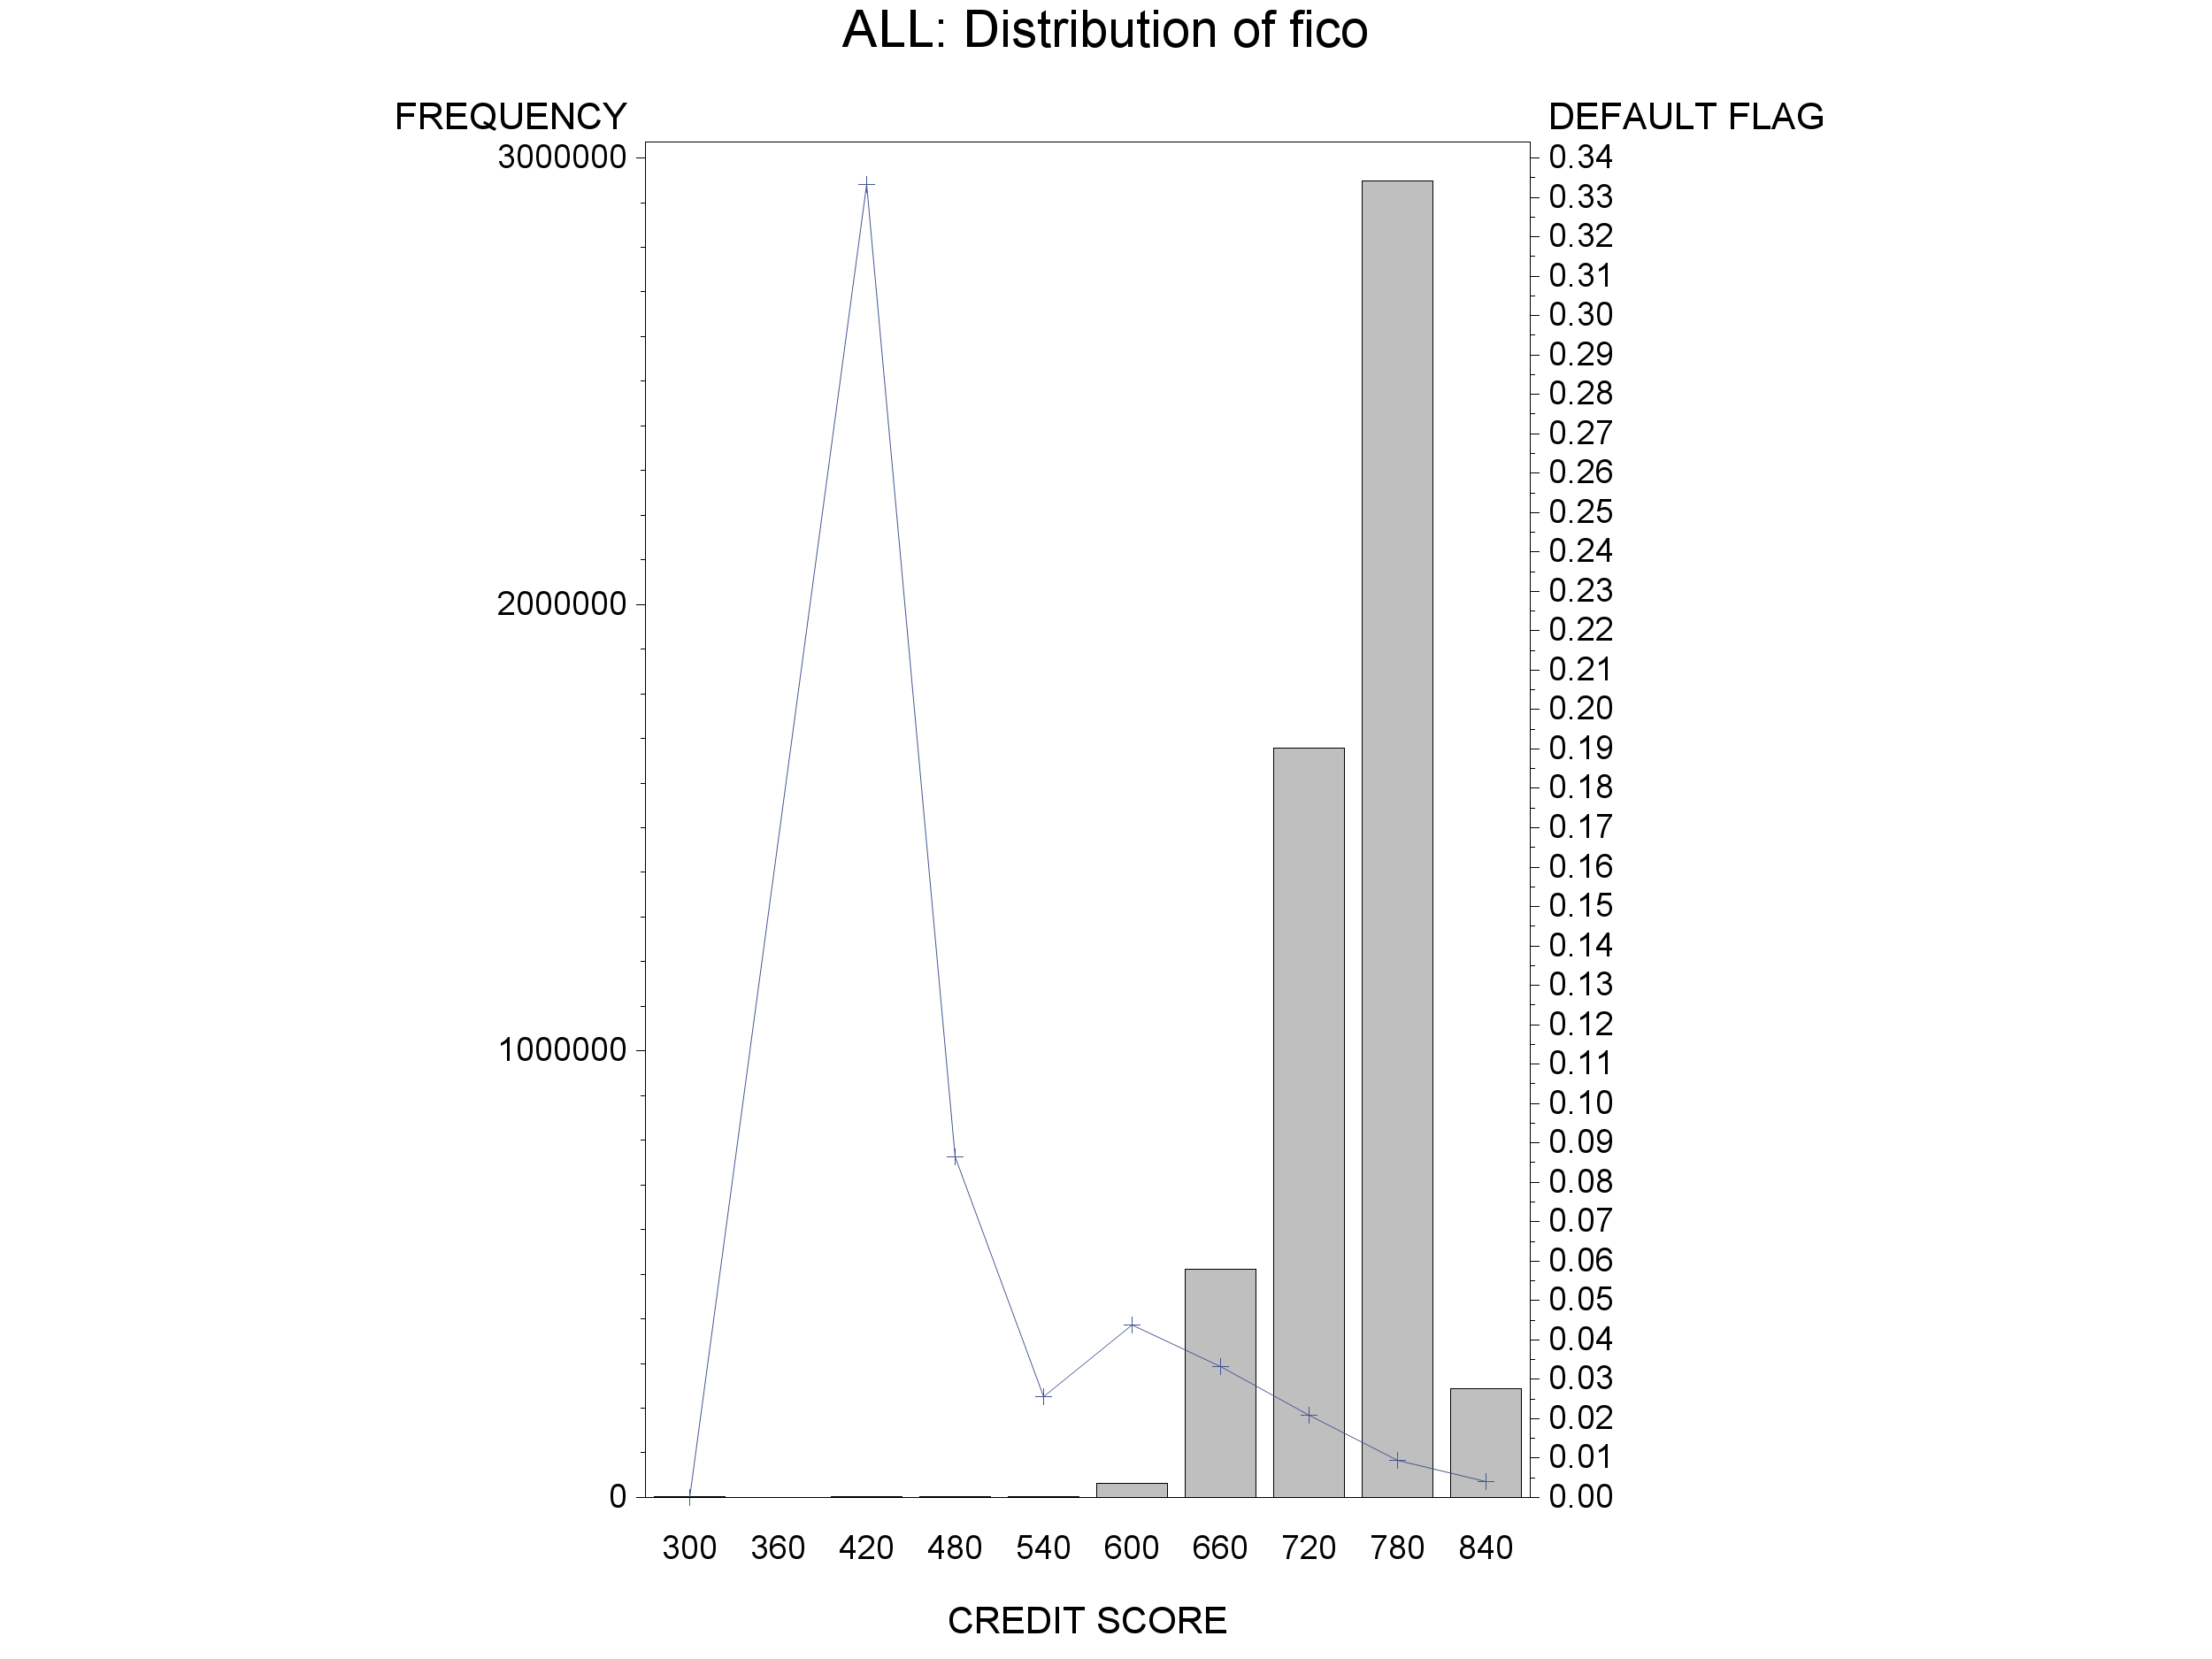
\includegraphics[width=0.9\textwidth]{./plot/Distribution/Main/RE_NUM_fico_DISTRIBUTION_ALL.png}
\end{minipage}%
\begin{minipage}{.5\textwidth}
	\centering
	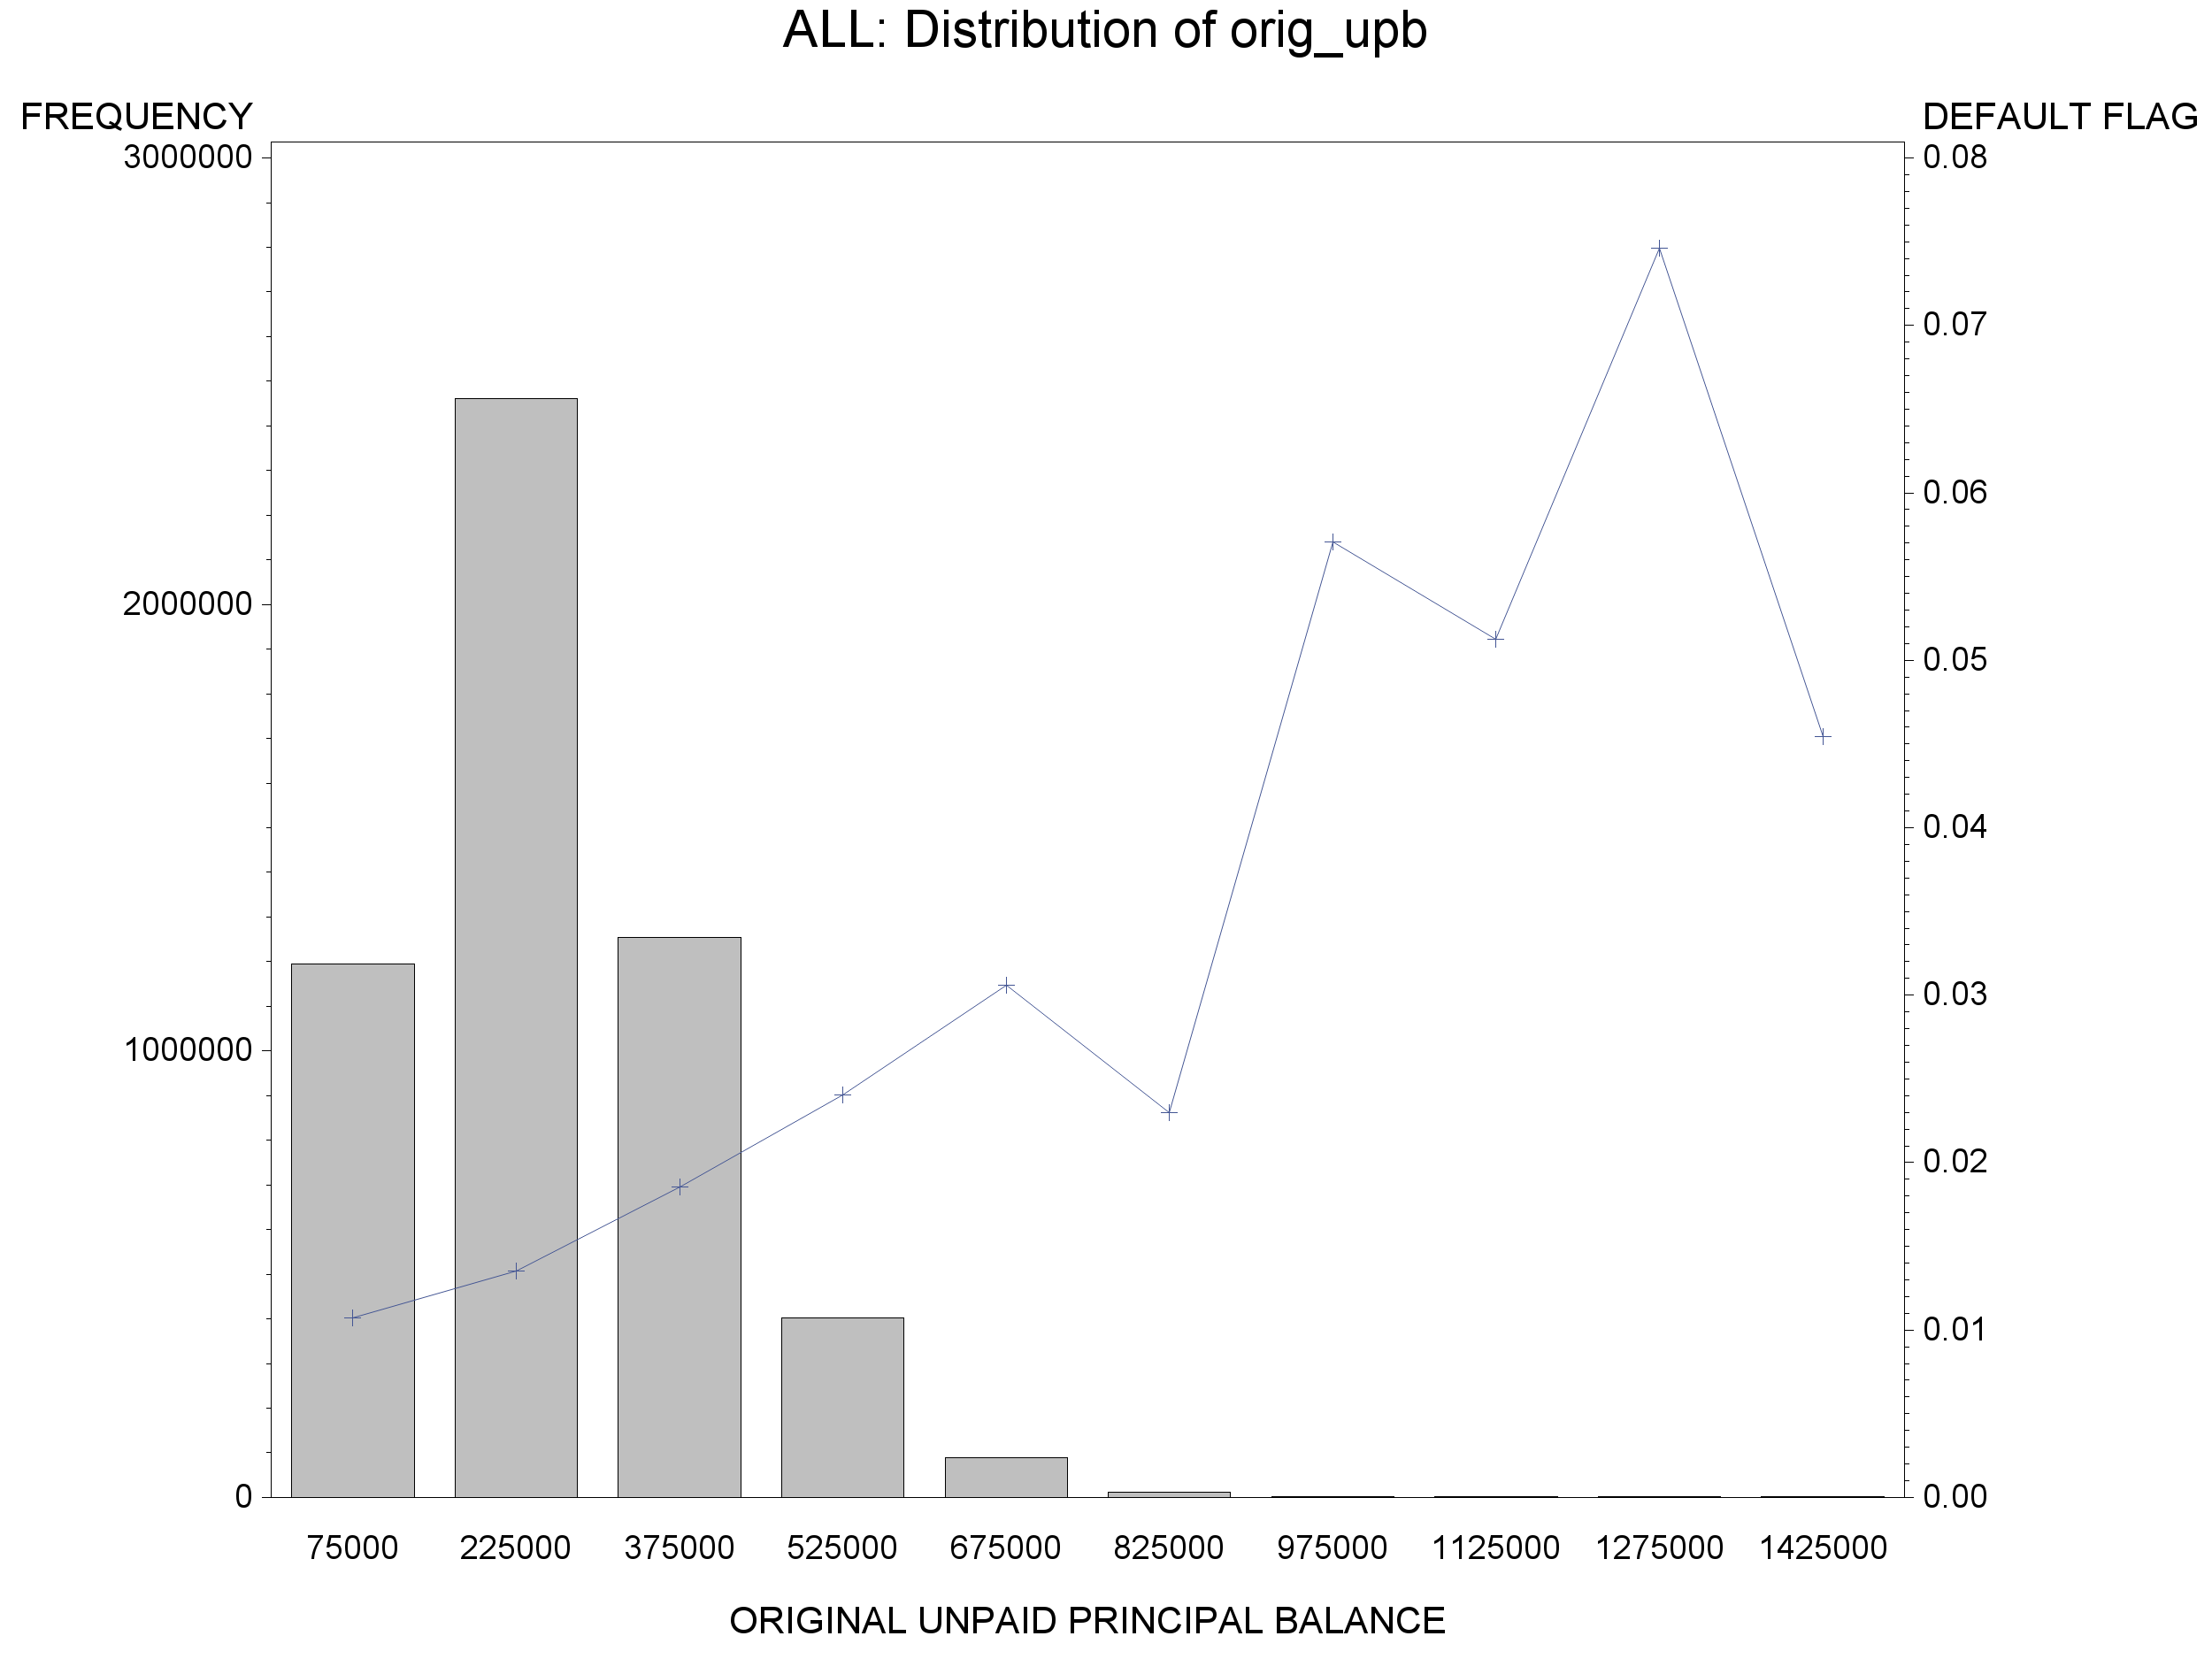
\includegraphics[width=0.9\textwidth]{./plot/Distribution/Main/RE_NUM_orig_upb_DISTRIBUTION_ALL.png}
\end{minipage}
    \caption{Distribution and default rate of Credit Score and UPB}
\end{figure}

\begin{figure}[H]
\begin{minipage}{.5\textwidth}
	\centering
	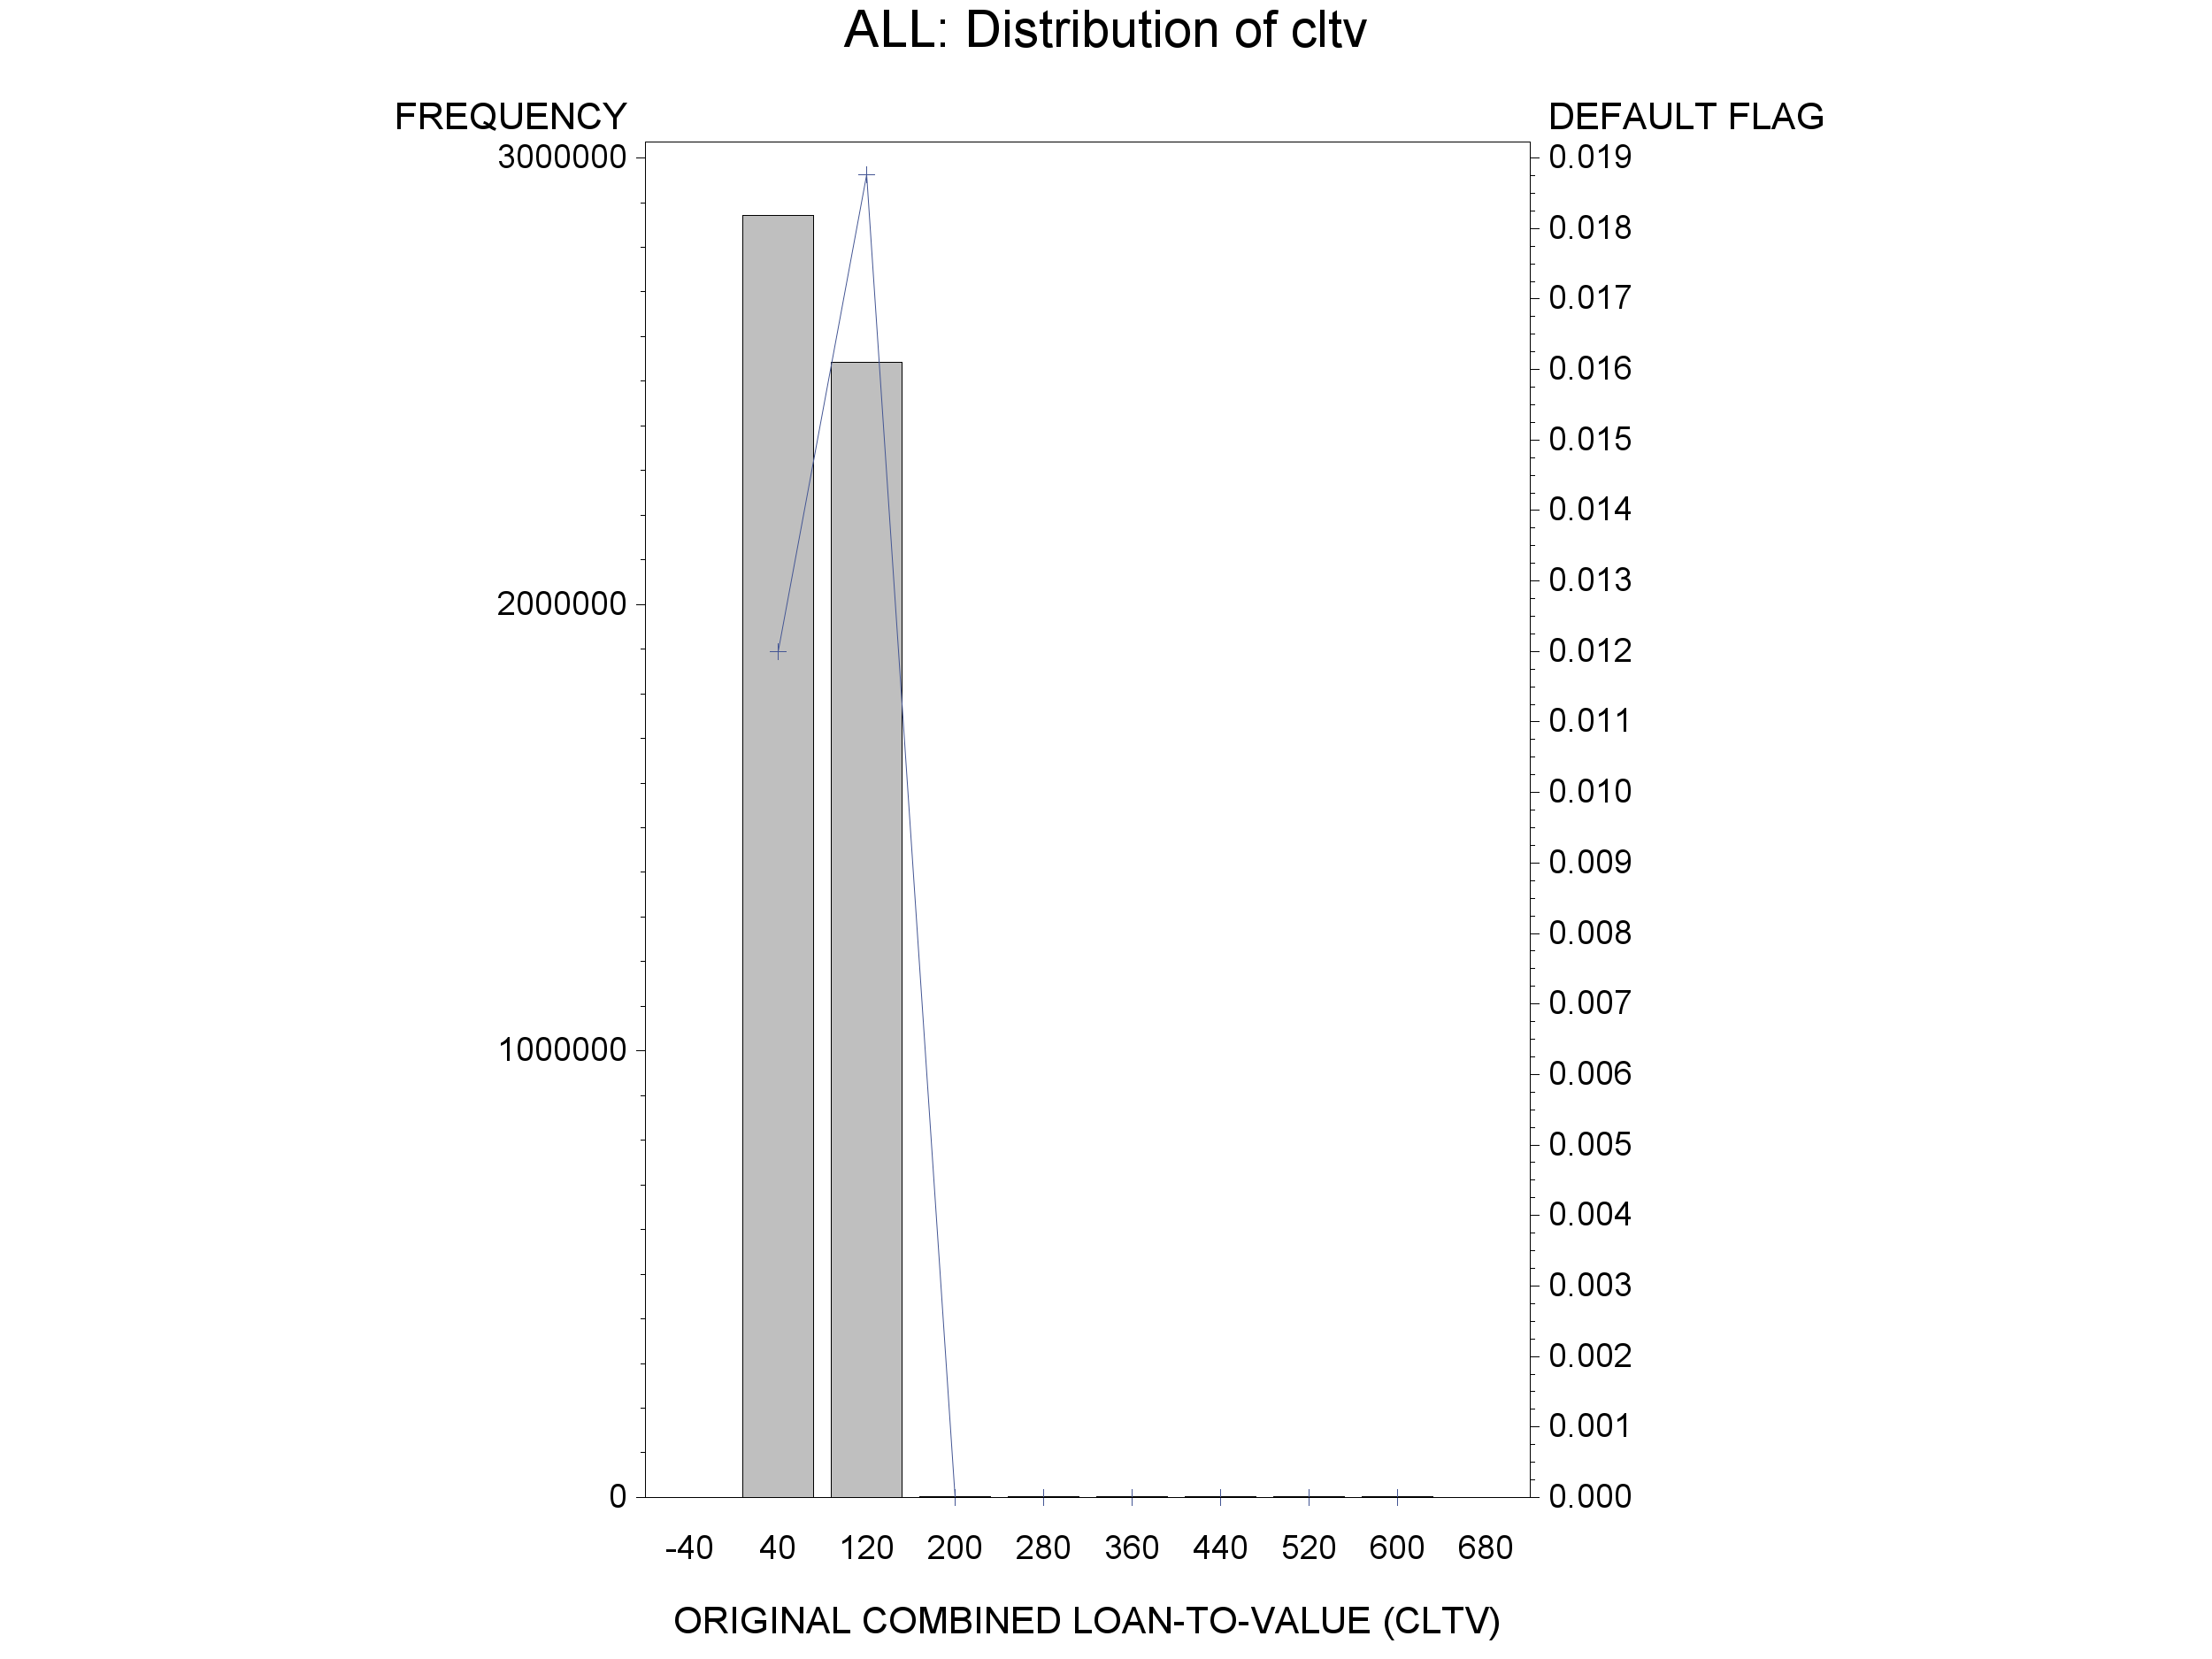
\includegraphics[width=0.9\textwidth]{./plot/Distribution/Main/RE_NUM_cltv_DISTRIBUTION_ALL.png}
\end{minipage}%
\begin{minipage}{.5\textwidth}
	\centering
	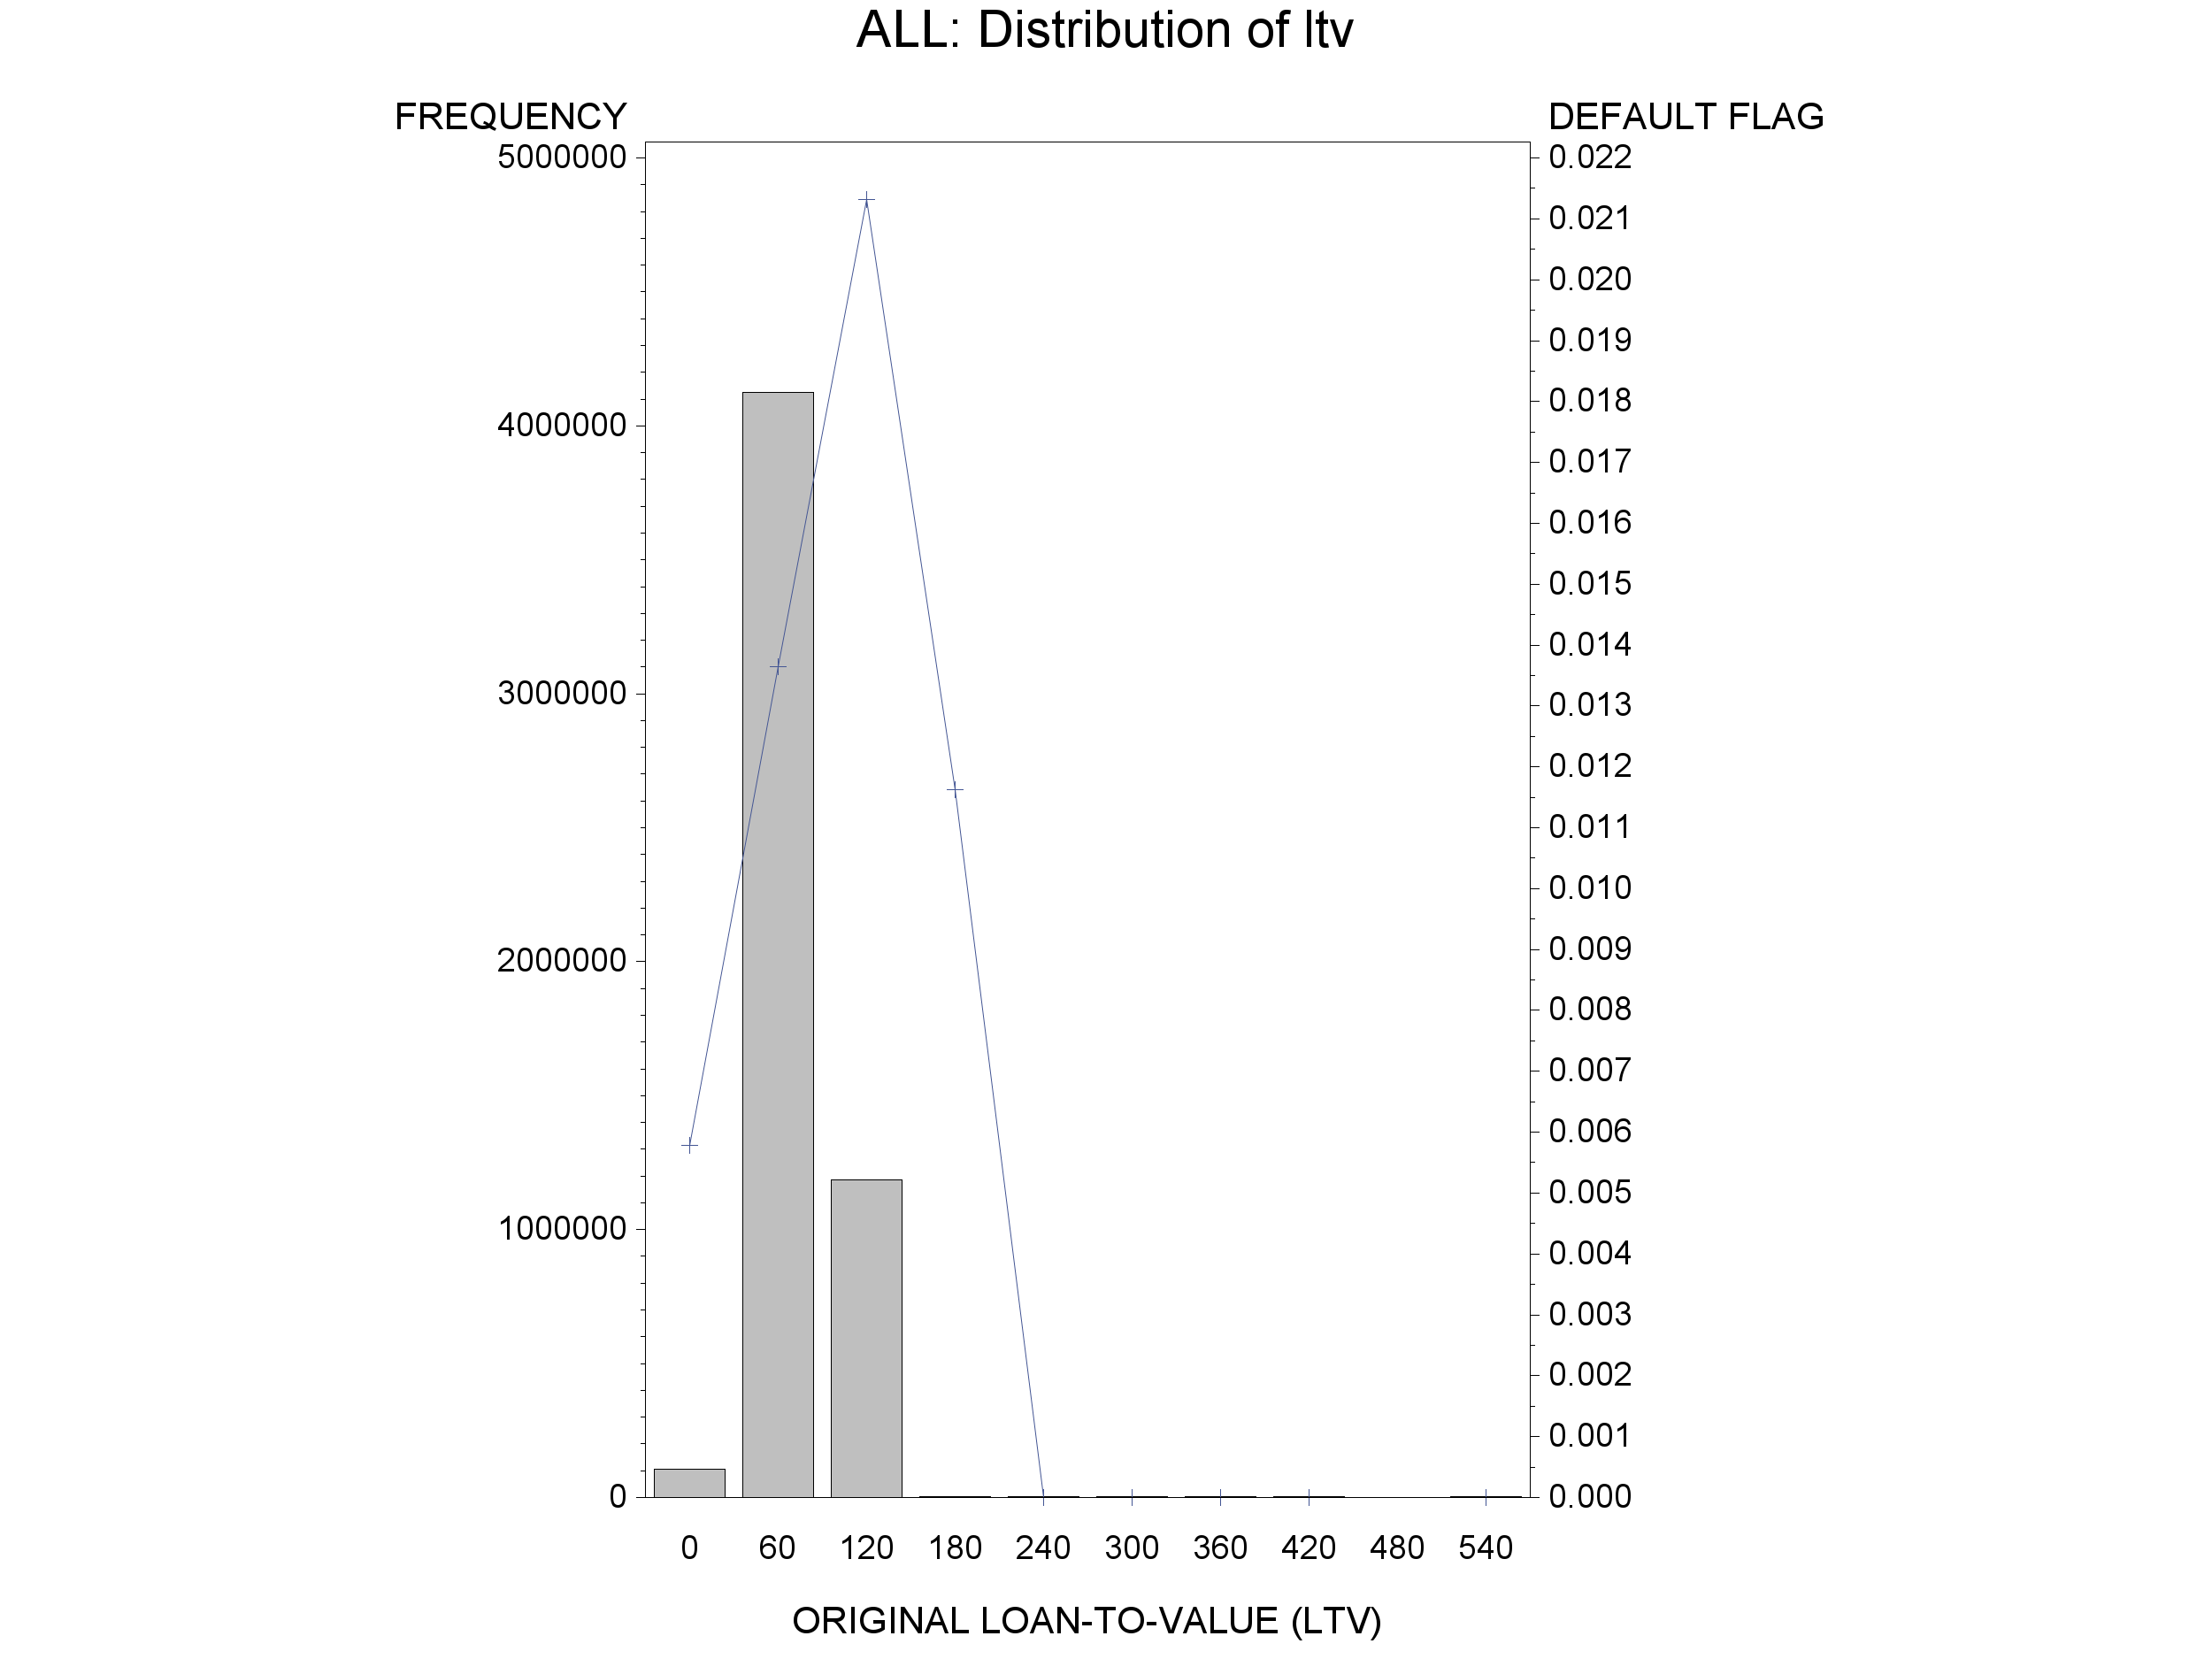
\includegraphics[width=0.9\textwidth]{./plot/Distribution/NUM_ltv_DISTRIBUTION_ALL.png}
\end{minipage}
    \caption{Distribution and default rate of CLTV and LTV}
\end{figure}

\begin{figure}[H]
\begin{minipage}{.5\textwidth}
	\centering
	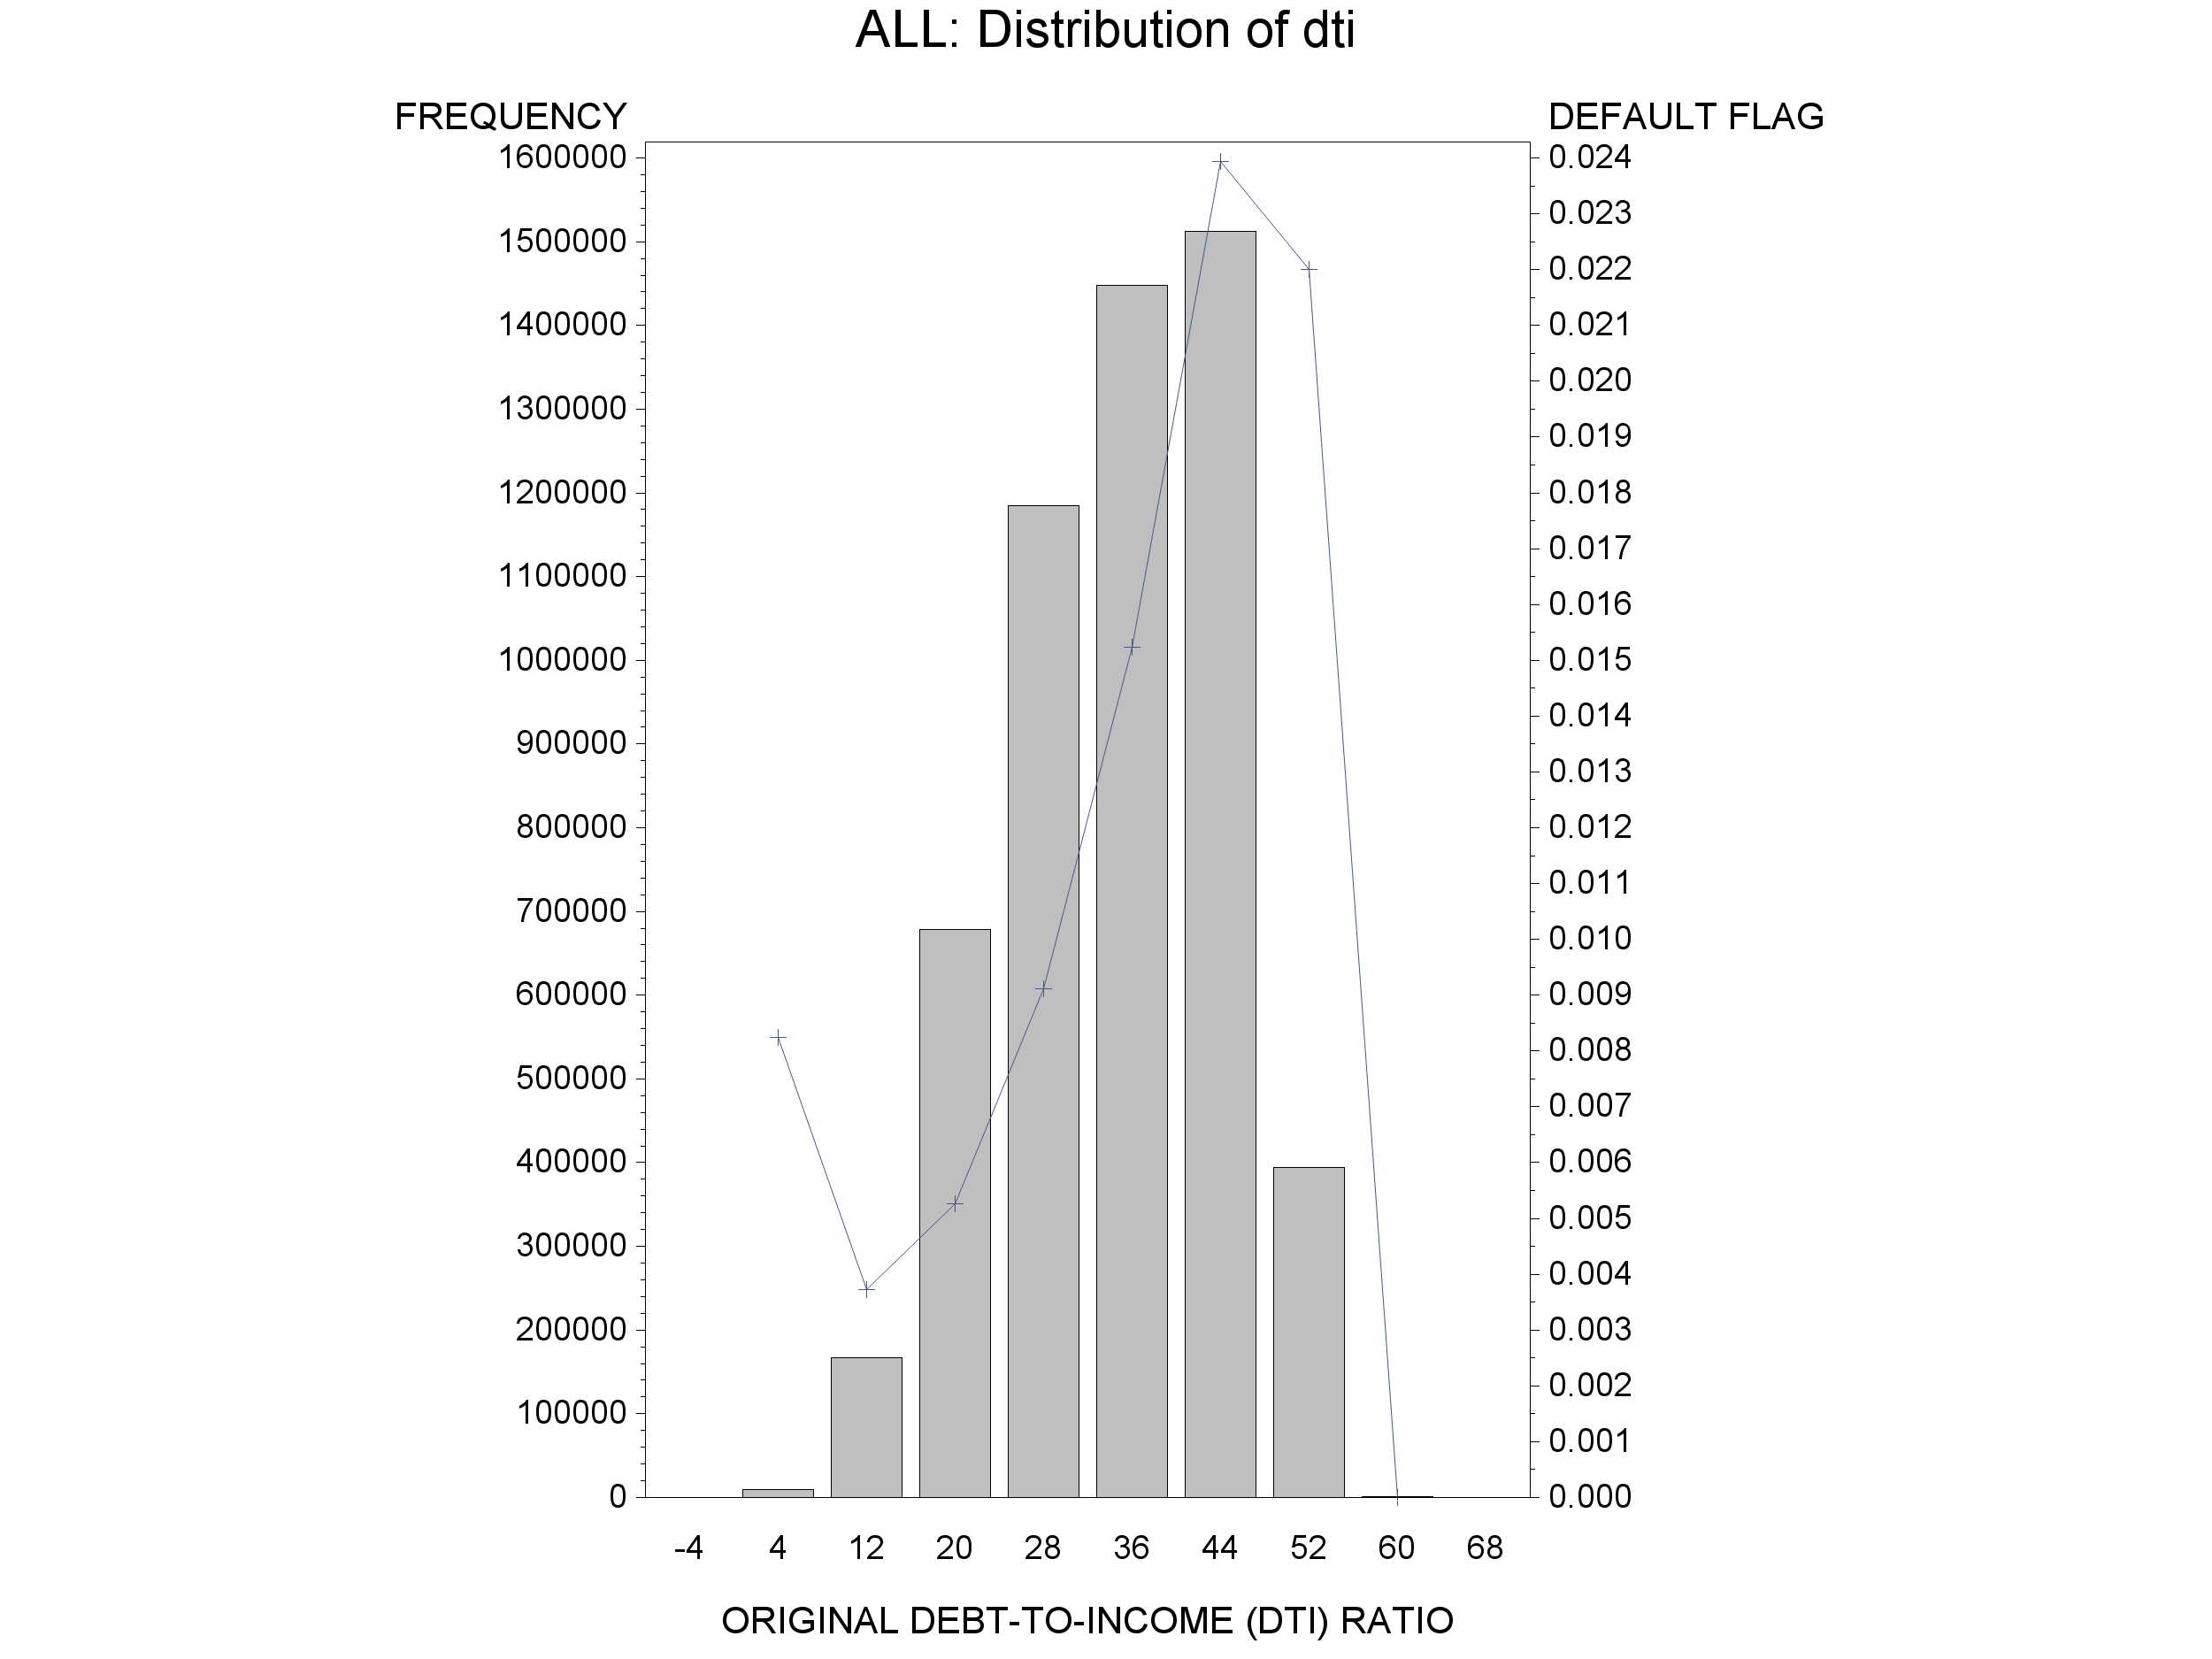
\includegraphics[width=0.9\textwidth]{./plot/Distribution/Main/RE_NUM_dti_DISTRIBUTION_ALL.png}
\end{minipage}%
\begin{minipage}{.5\textwidth}
	\centering
	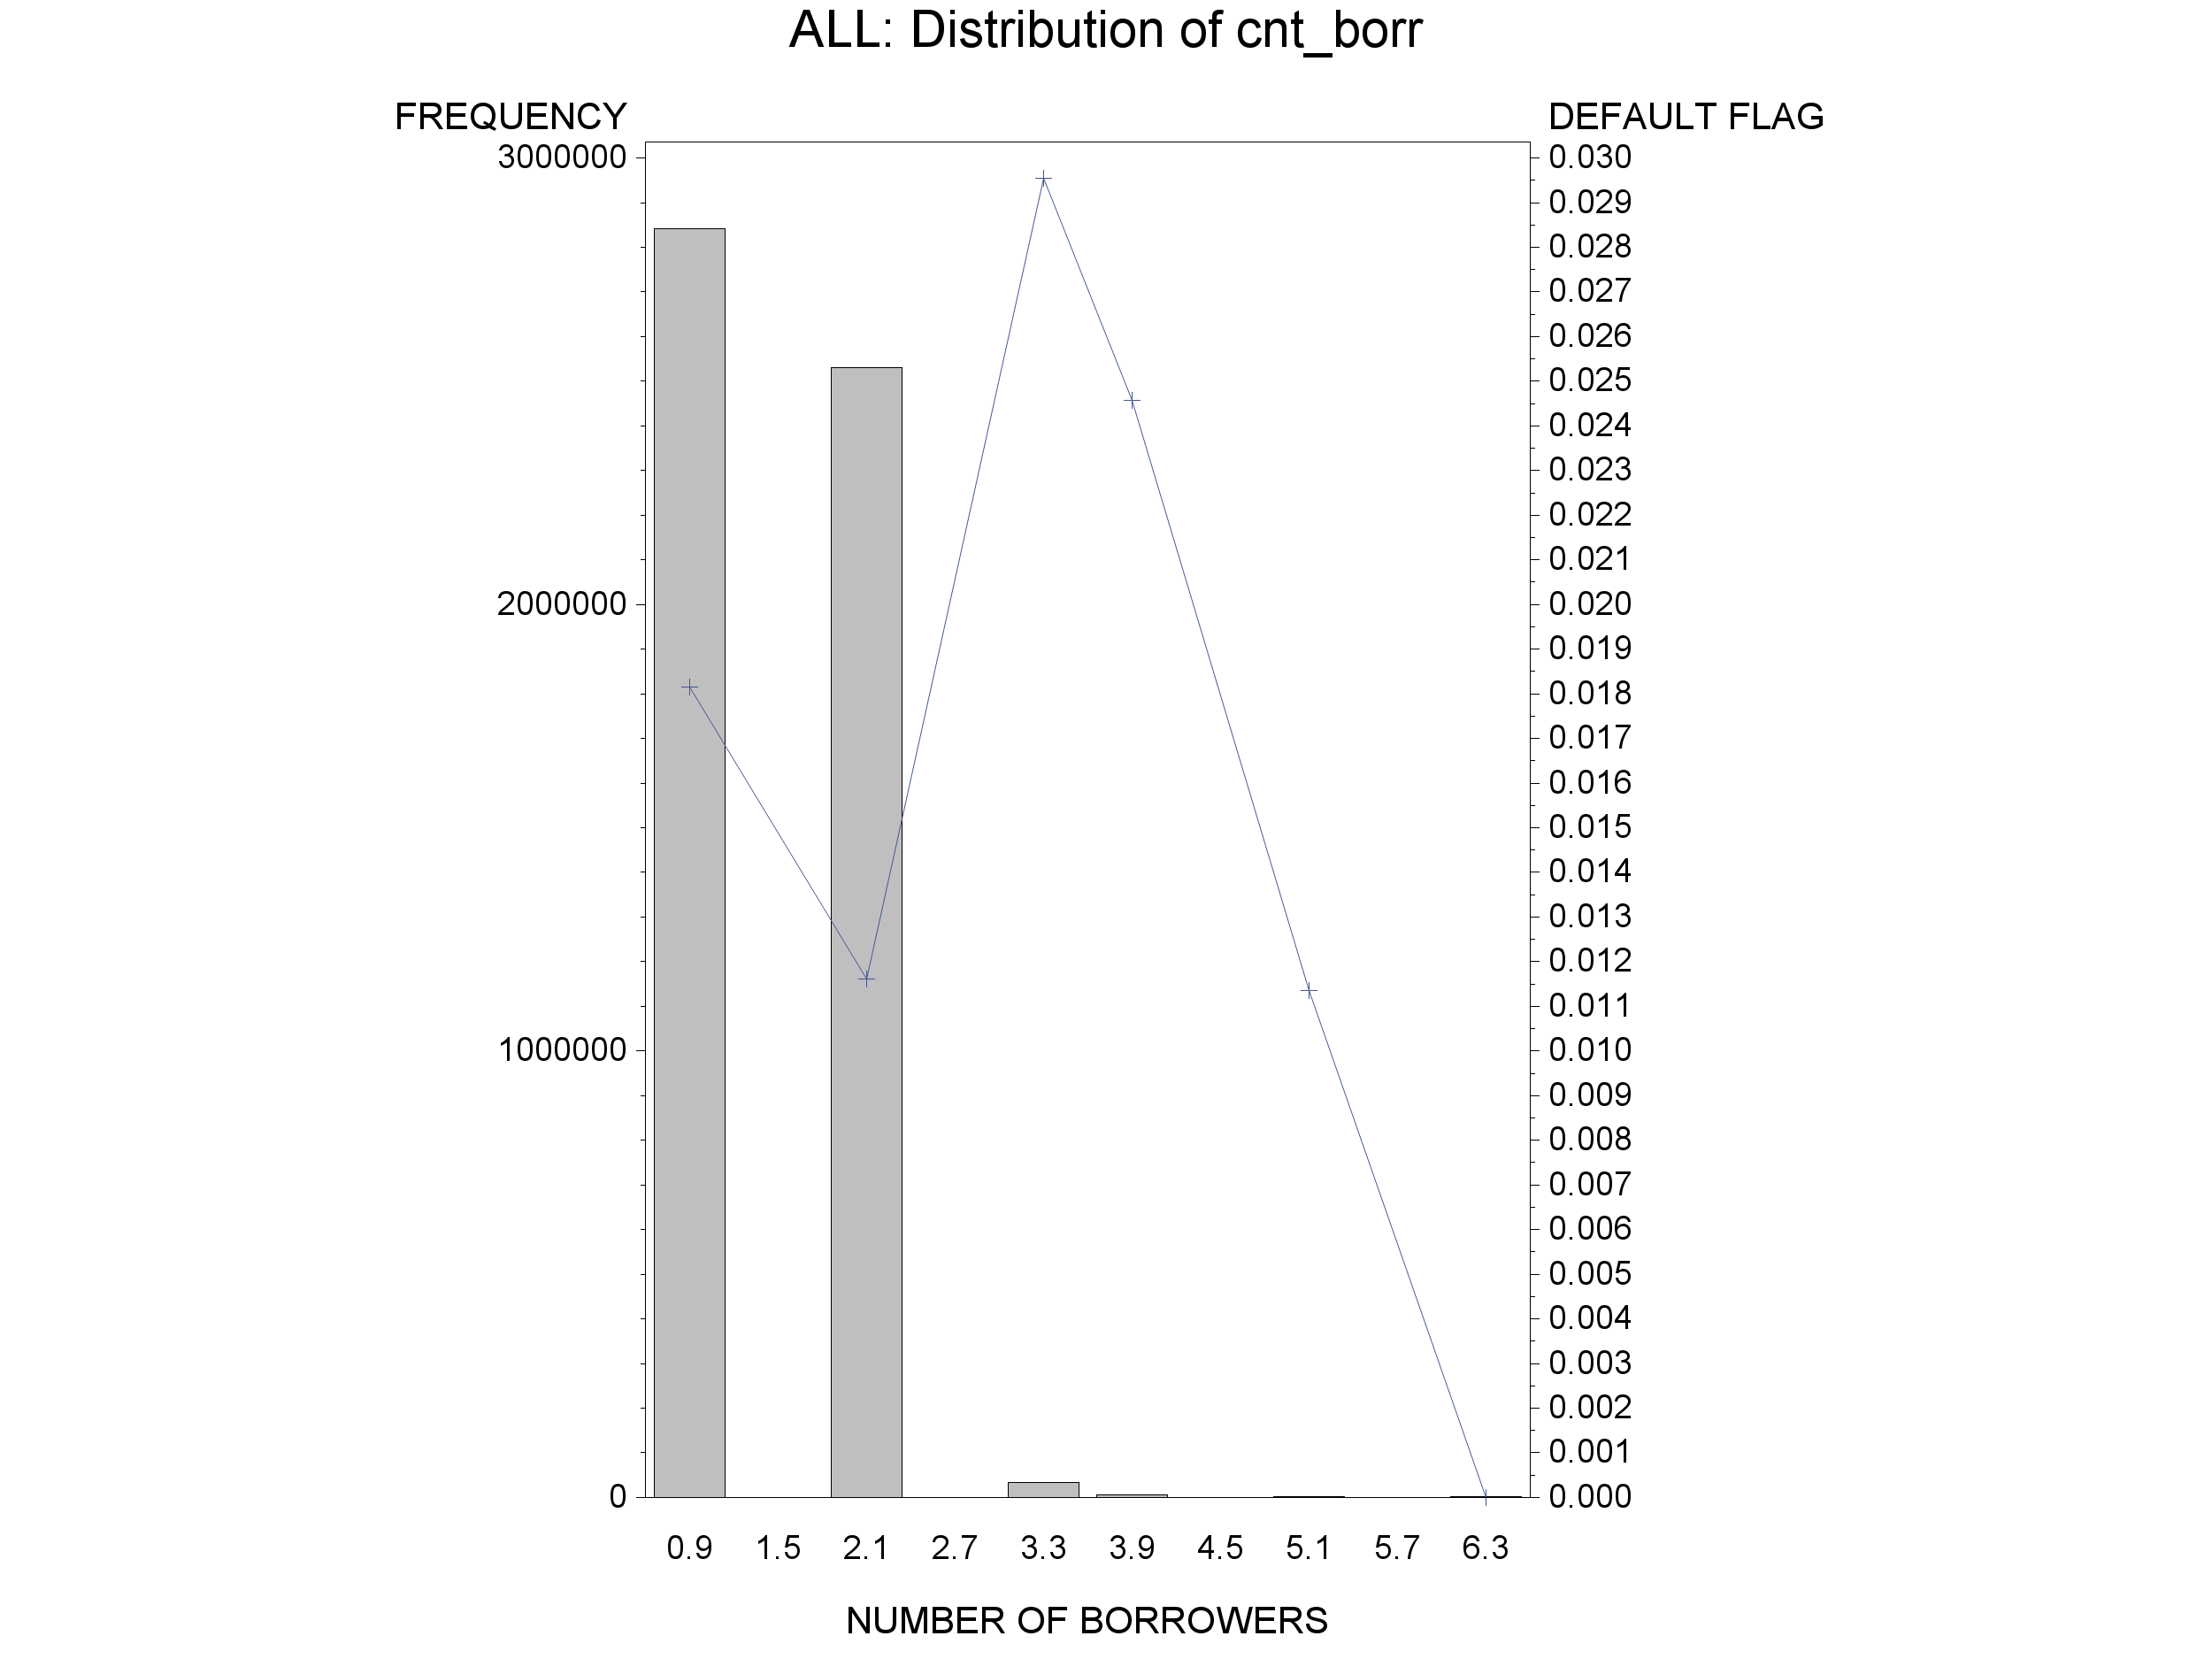
\includegraphics[width=0.9\textwidth]{./plot/Distribution/Main/RE_NUM_cnt_borr_DISTRIBUTION_ALL.png}
\end{minipage}
    \caption{Distribution and default rate of DTI and No Borrowers}
\end{figure}

\begin{figure}[H]
\begin{minipage}{.5\textwidth}
	\centering
	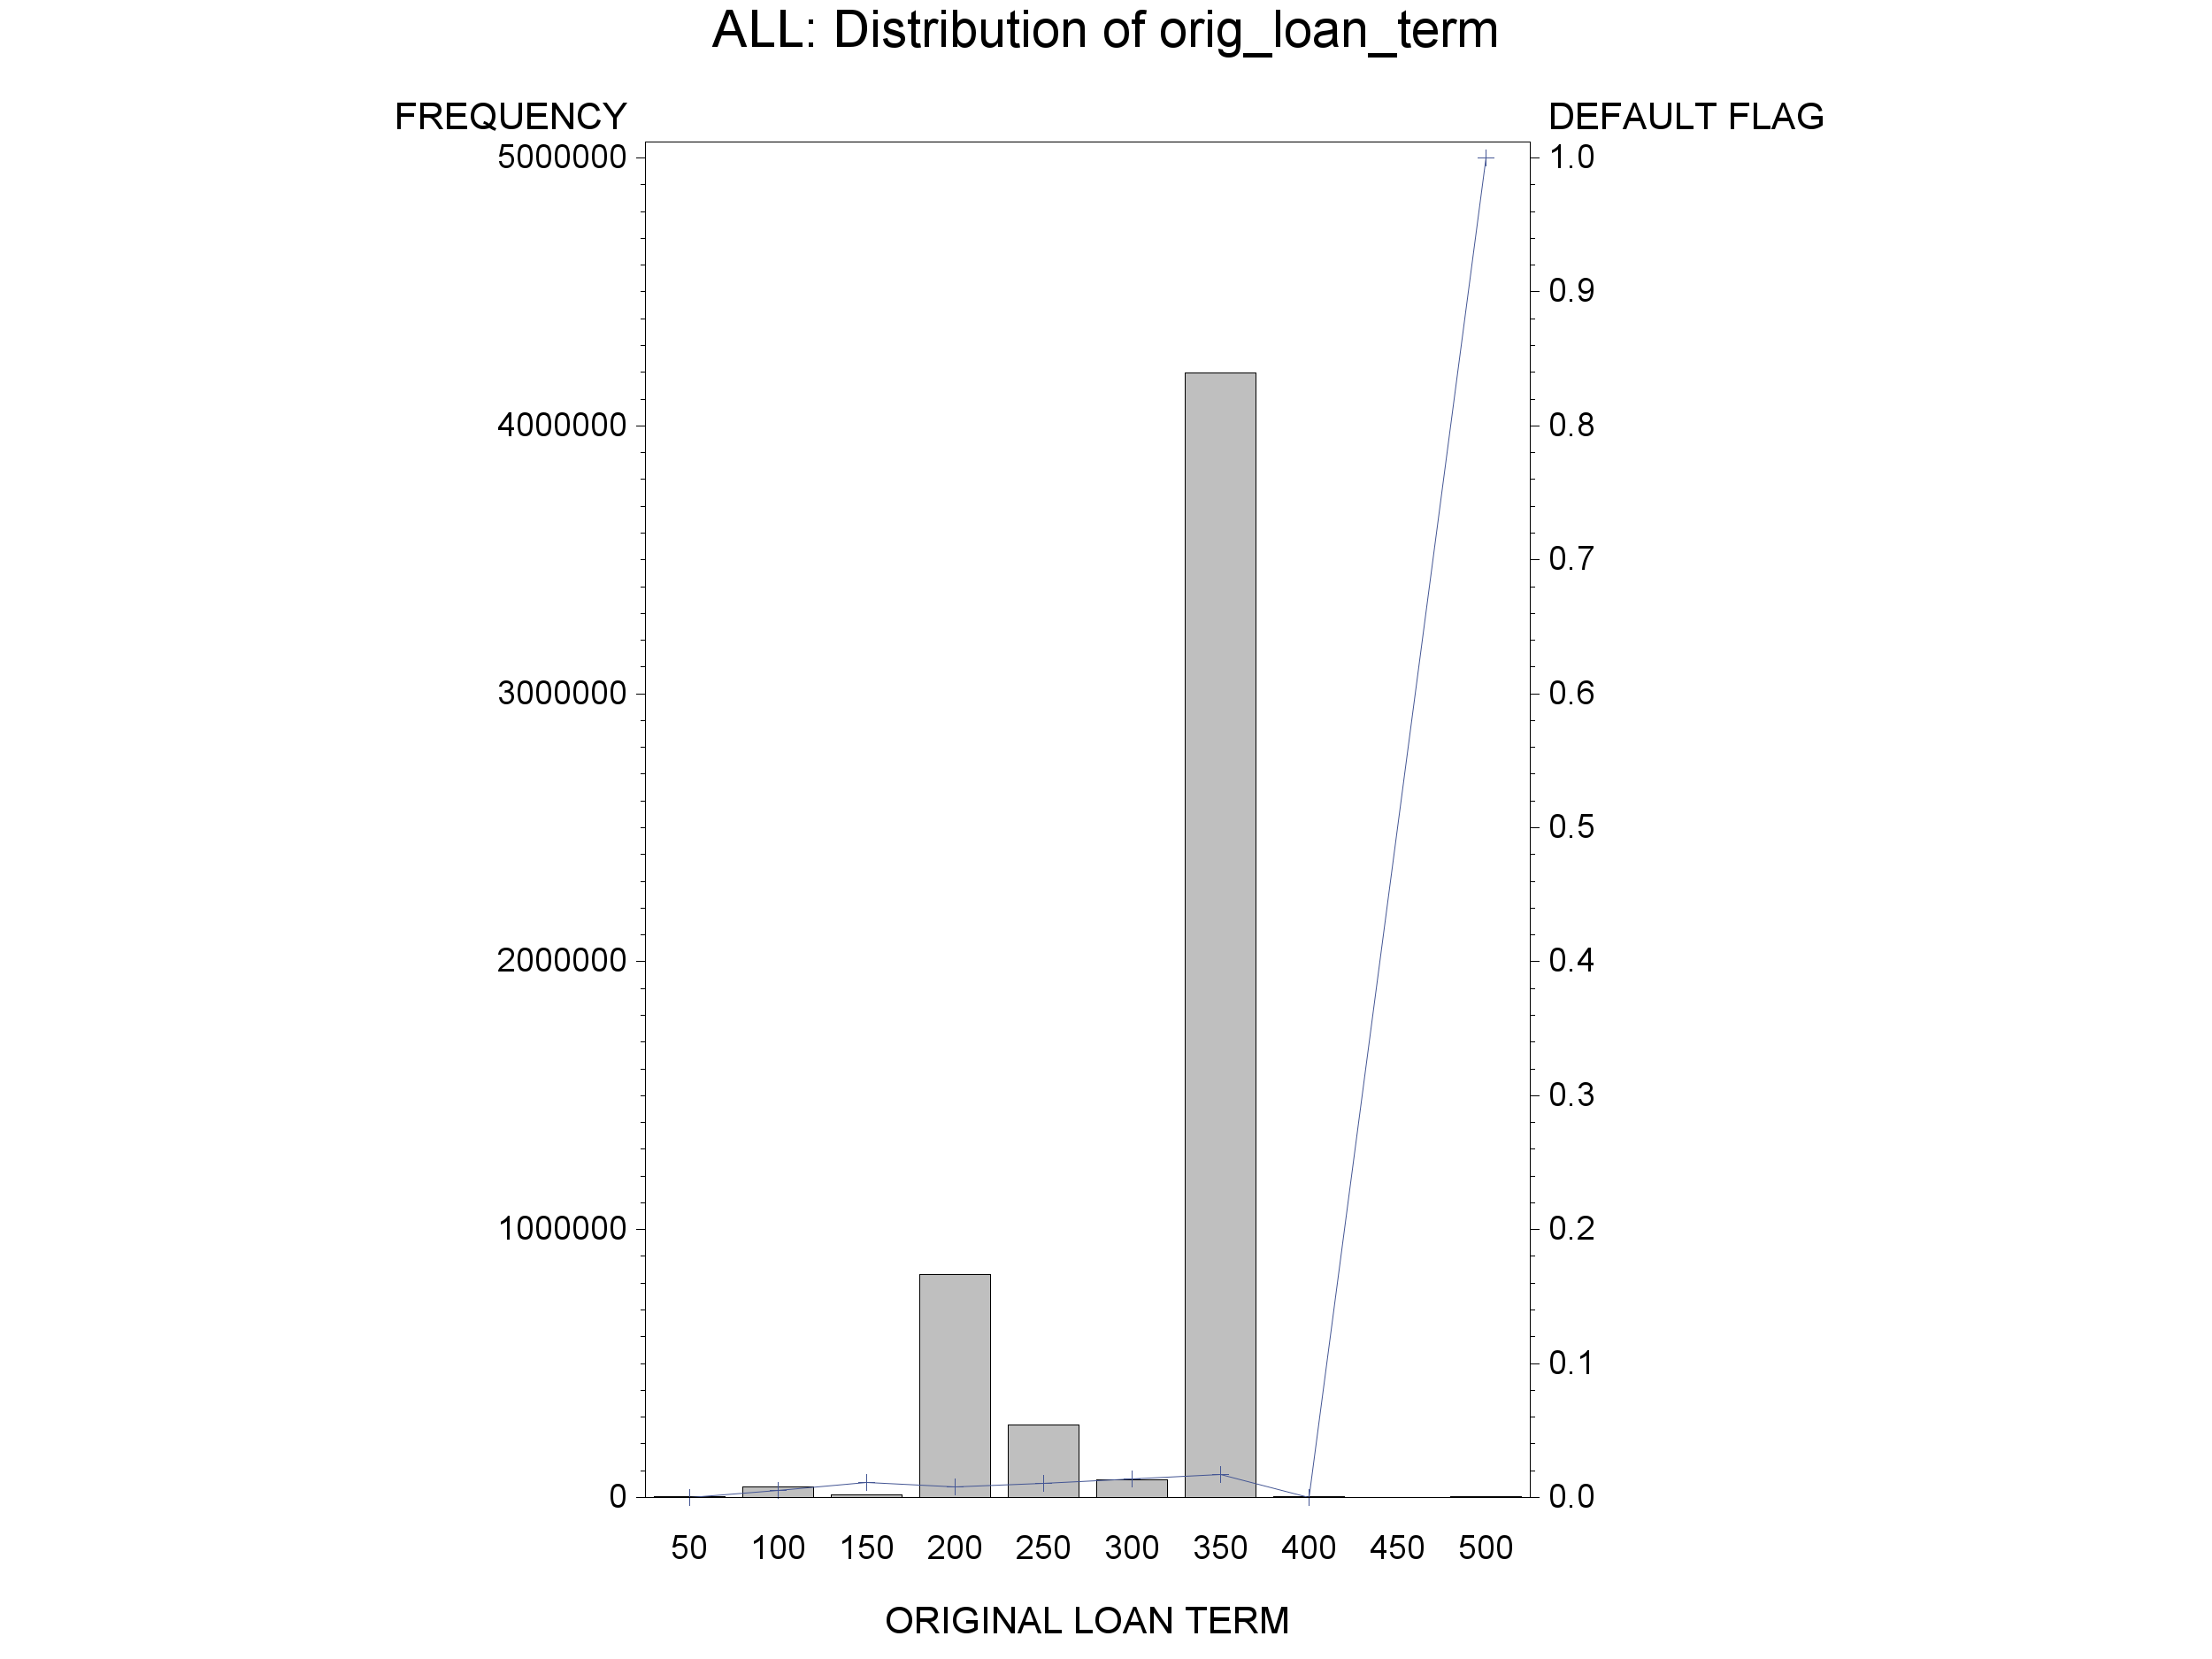
\includegraphics[width=0.9\textwidth]{./plot/Distribution/NUM_orig_loan_term_DISTRIBUTION_ALL.png}
\end{minipage}%
\begin{minipage}{.5\textwidth}
	\centering
	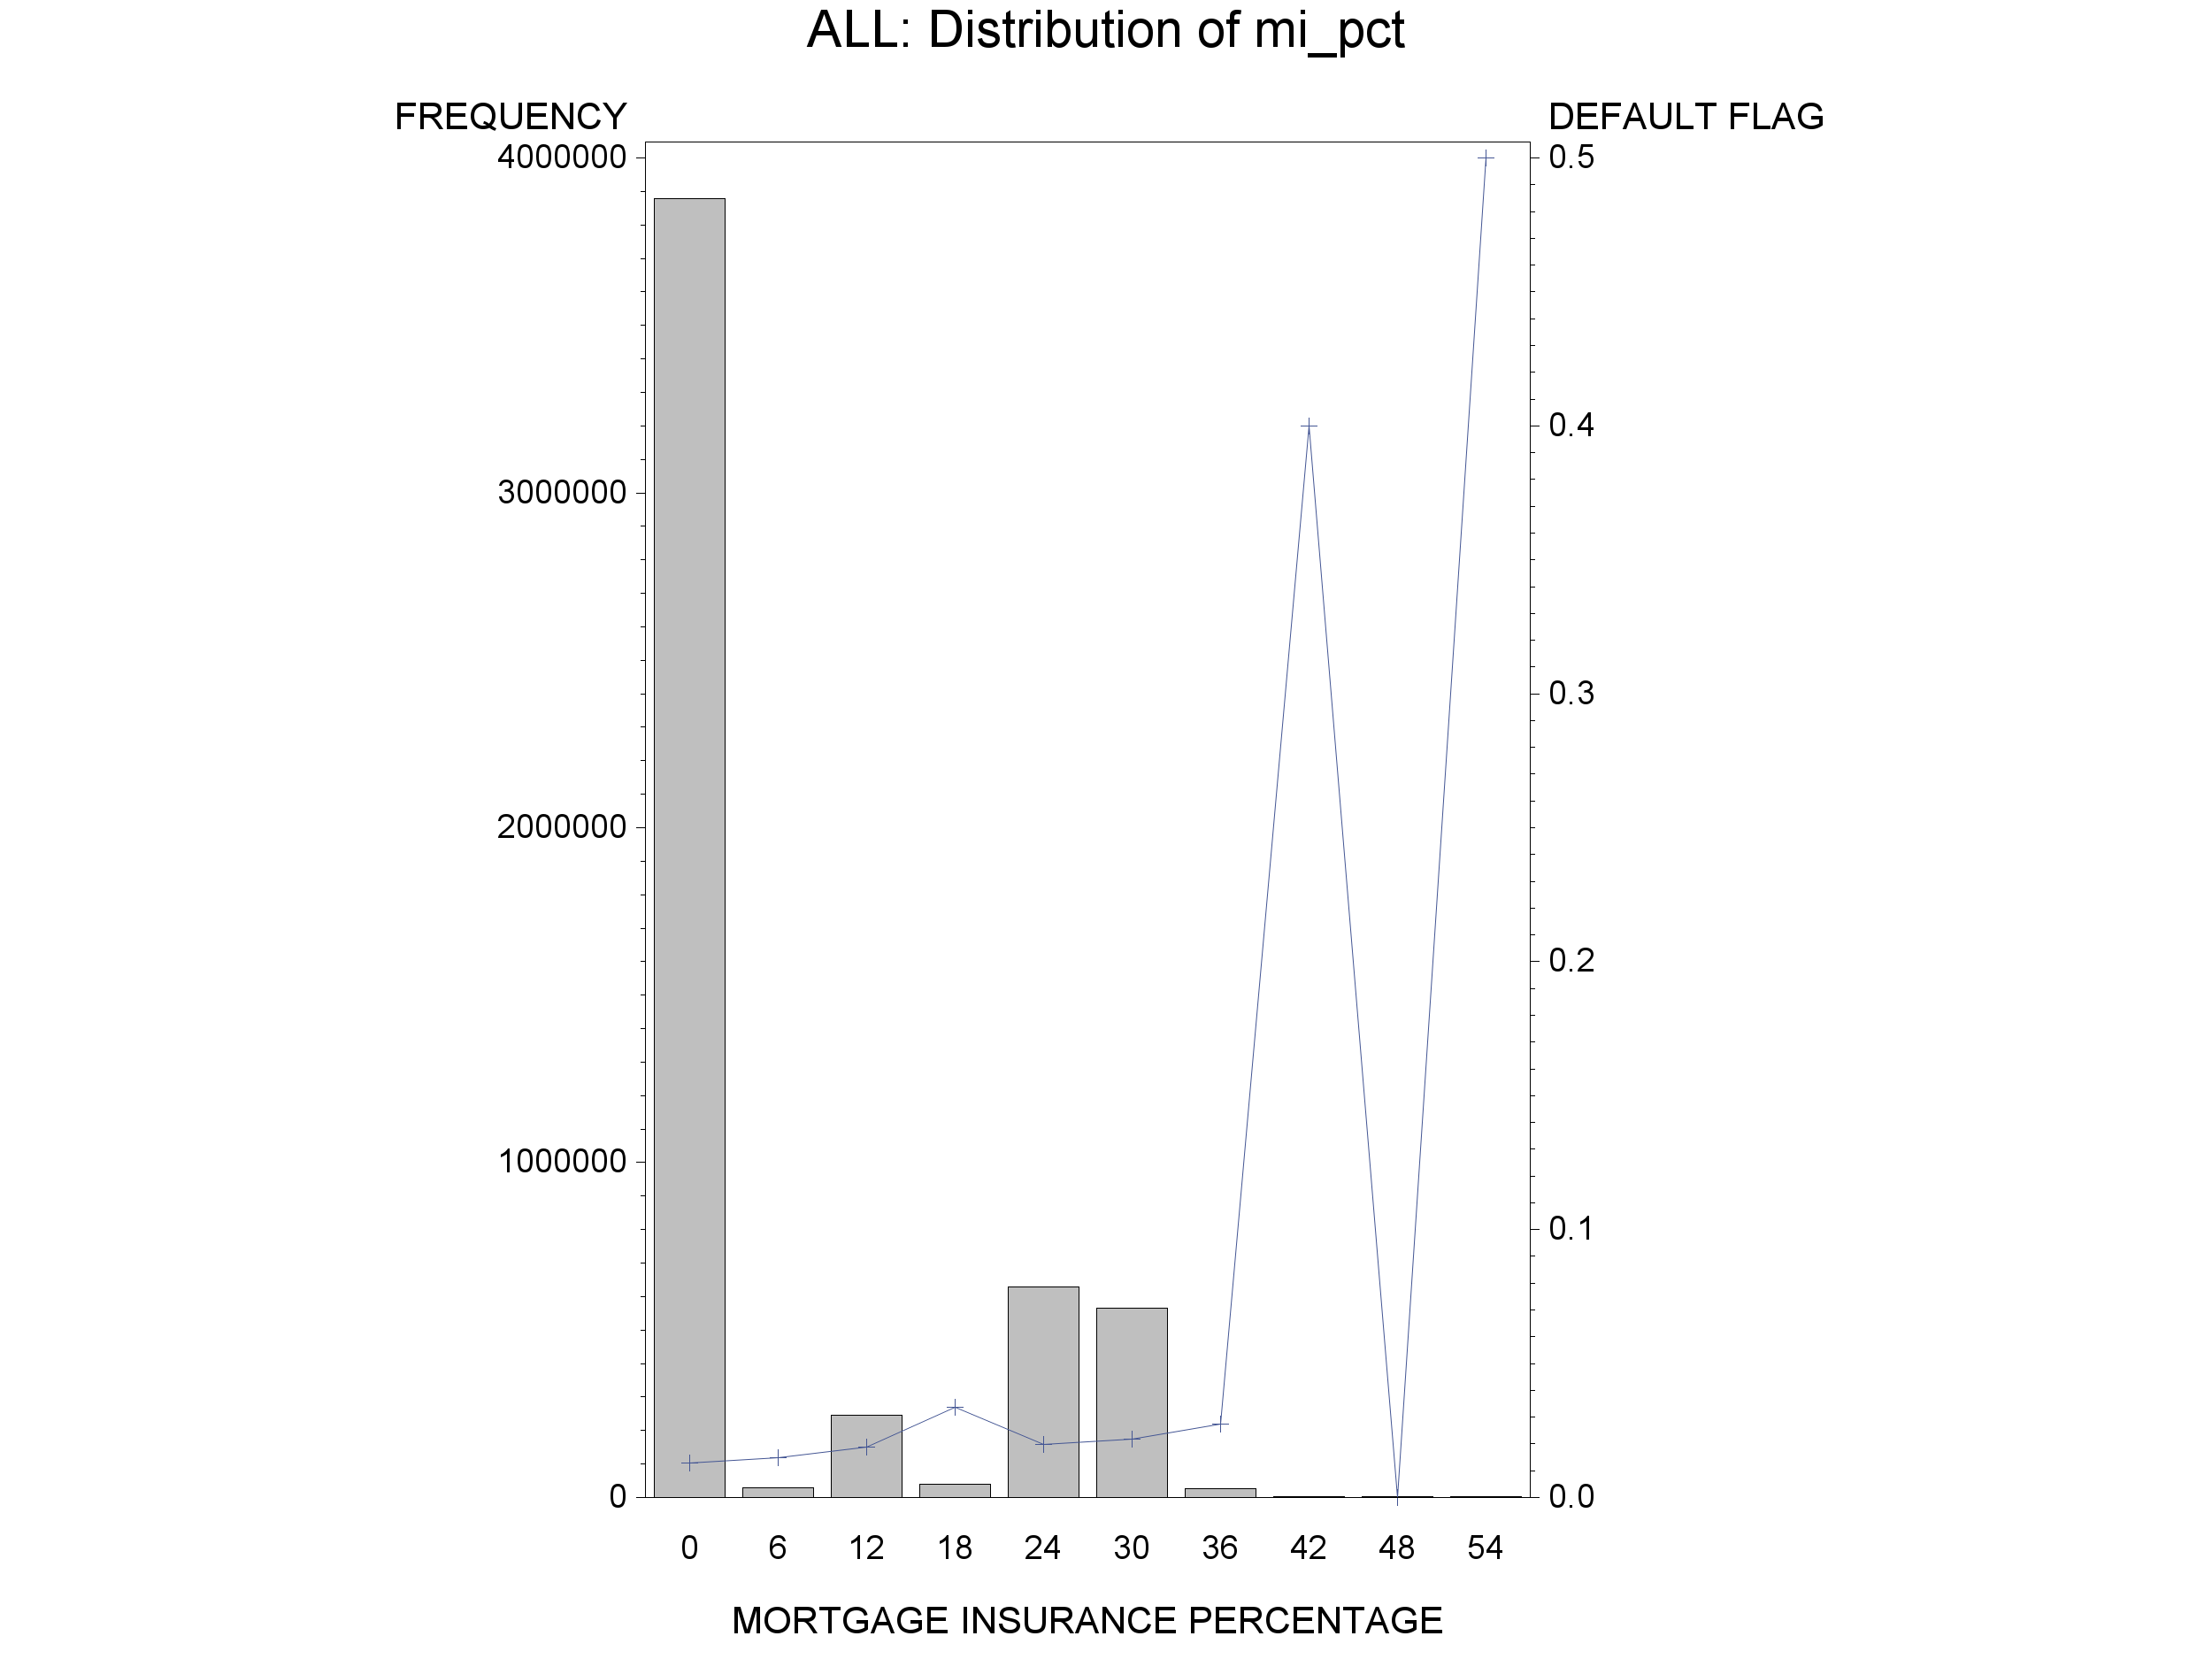
\includegraphics[width=0.9\textwidth]{./plot/Distribution/NUM_mi_pct_DISTRIBUTION_ALL.png}
\end{minipage}
    \caption{Distribution and default rate of Loan Term and MI Perc}
\end{figure}

\begin{figure}[H]
	\centering
	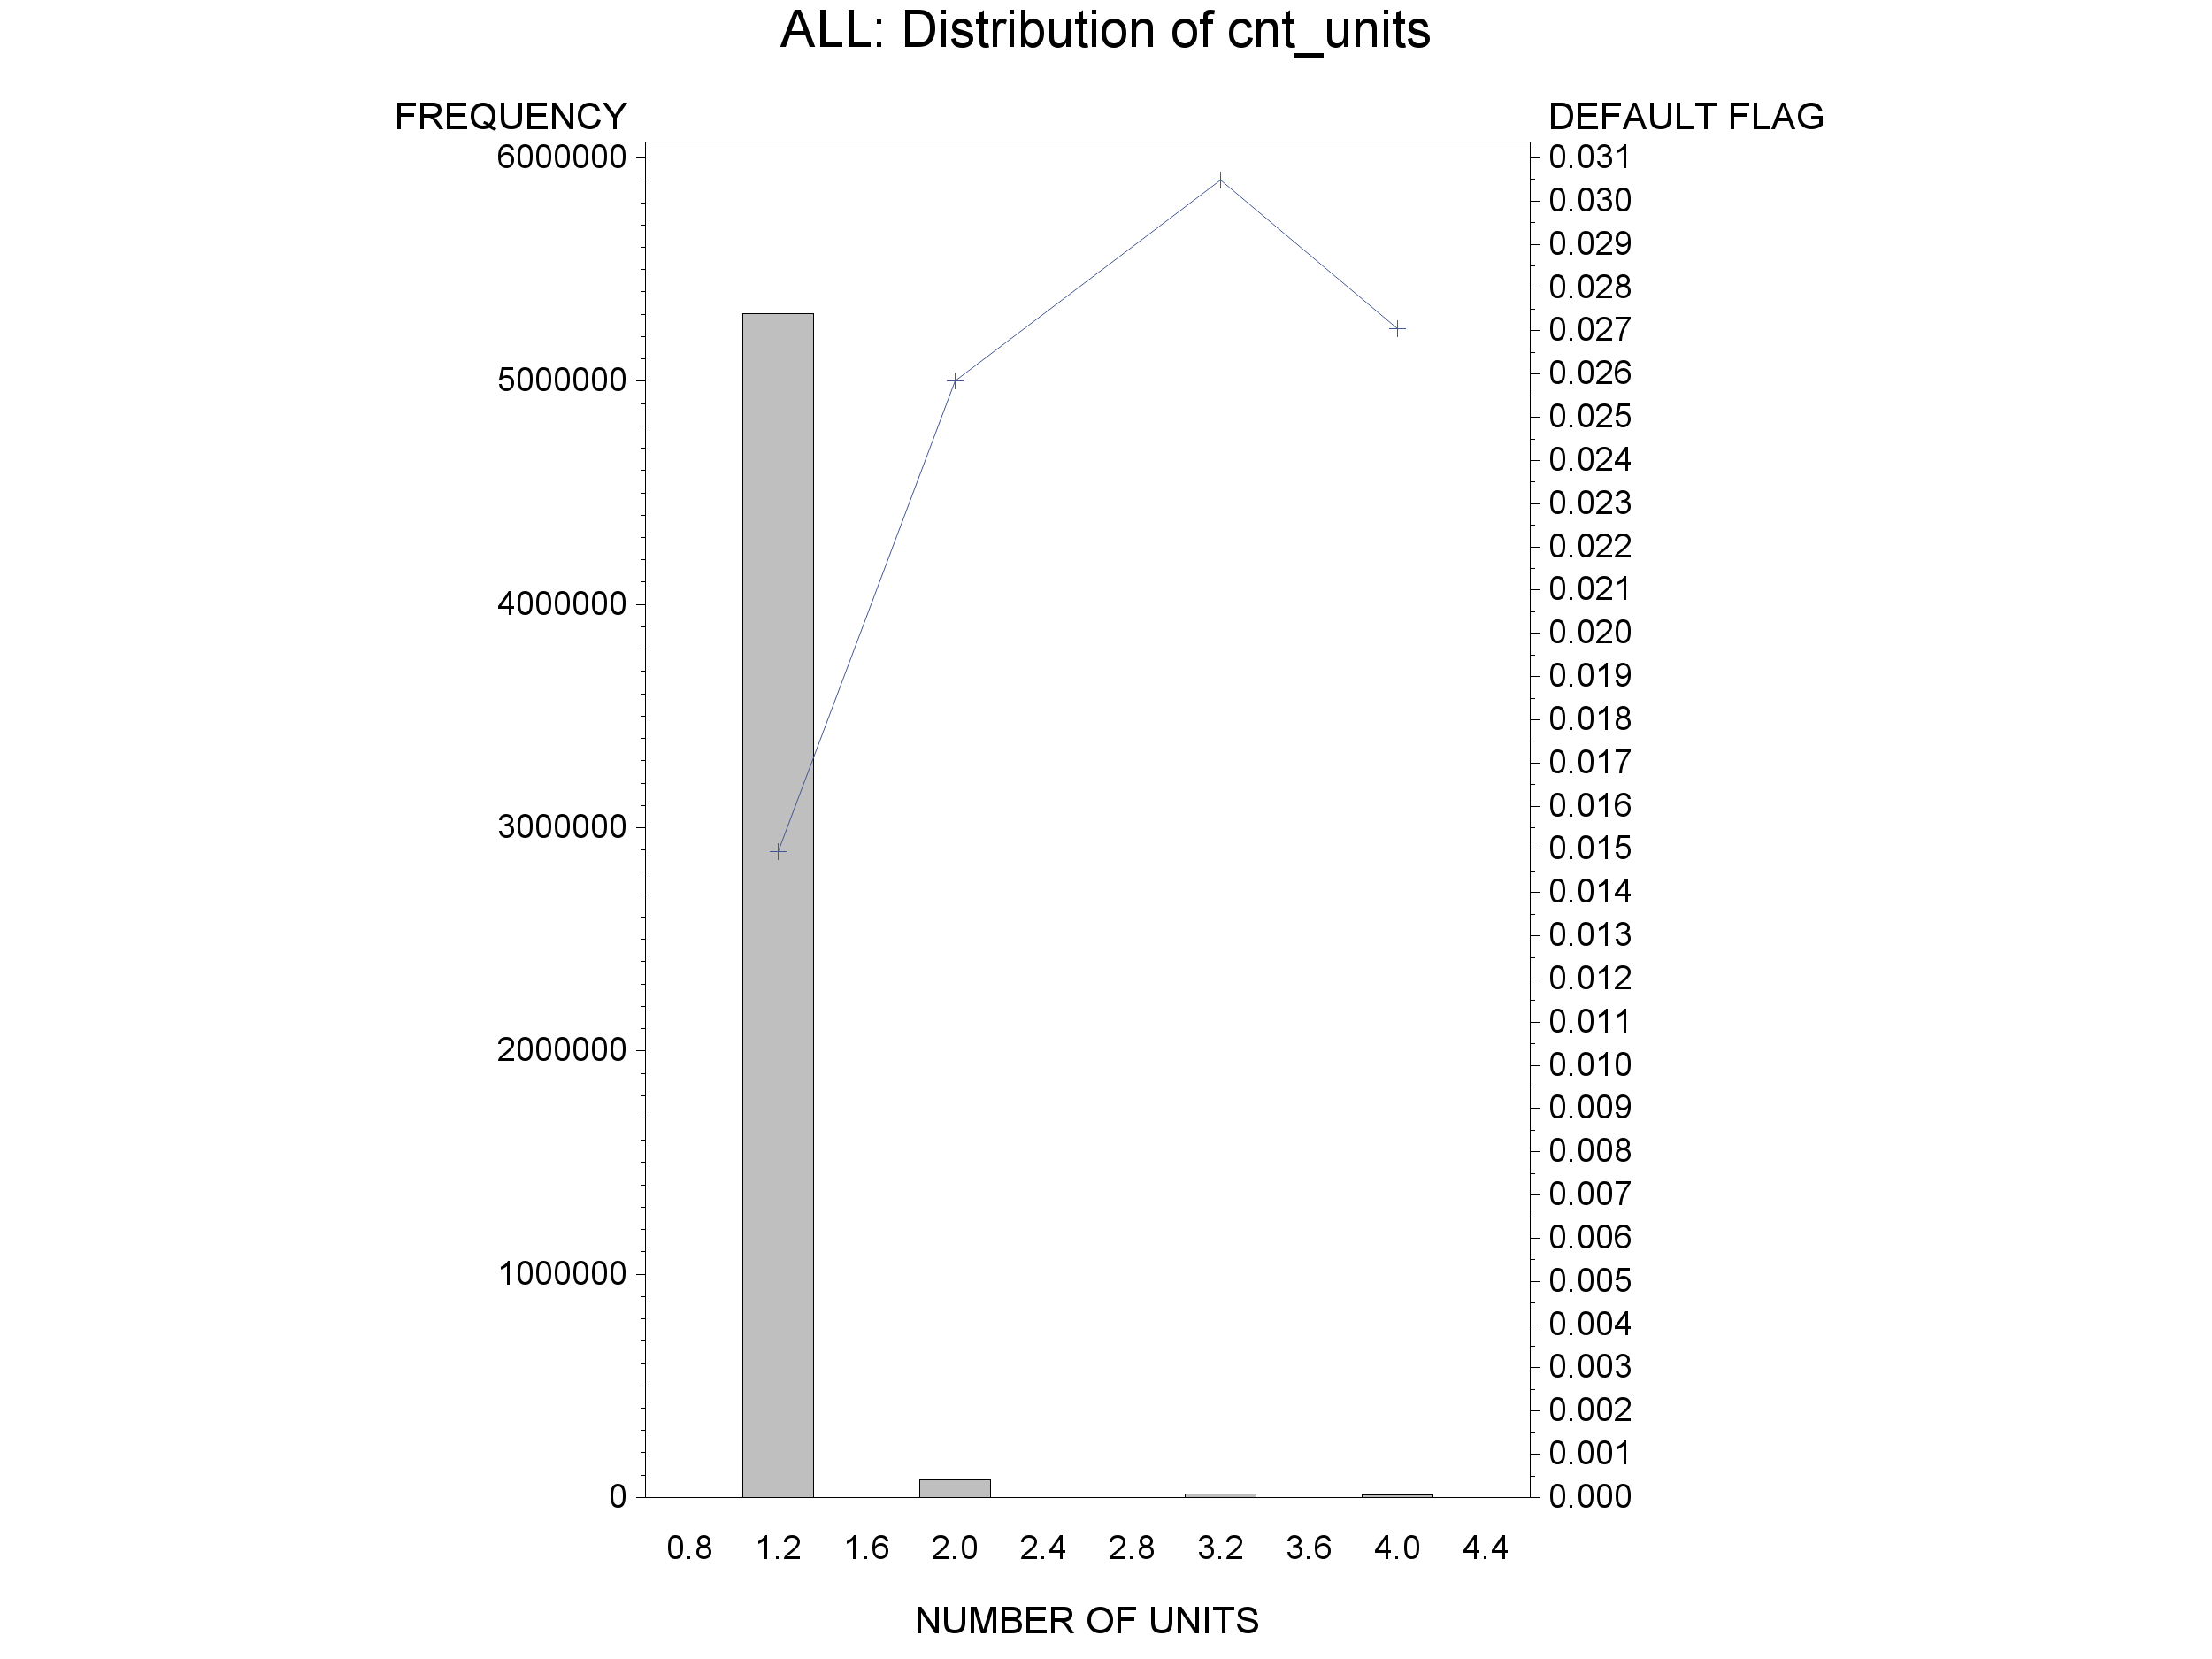
\includegraphics[width=0.5\textwidth]{./plot/Distribution/NUM_cnt_units_DISTRIBUTION_ALL.png}
    \caption{Distribution and default rate of No Units}
\end{figure}

\subsection{Categorical variables}

\begin{figure}[H]
\begin{minipage}{.5\textwidth}
	\centering
	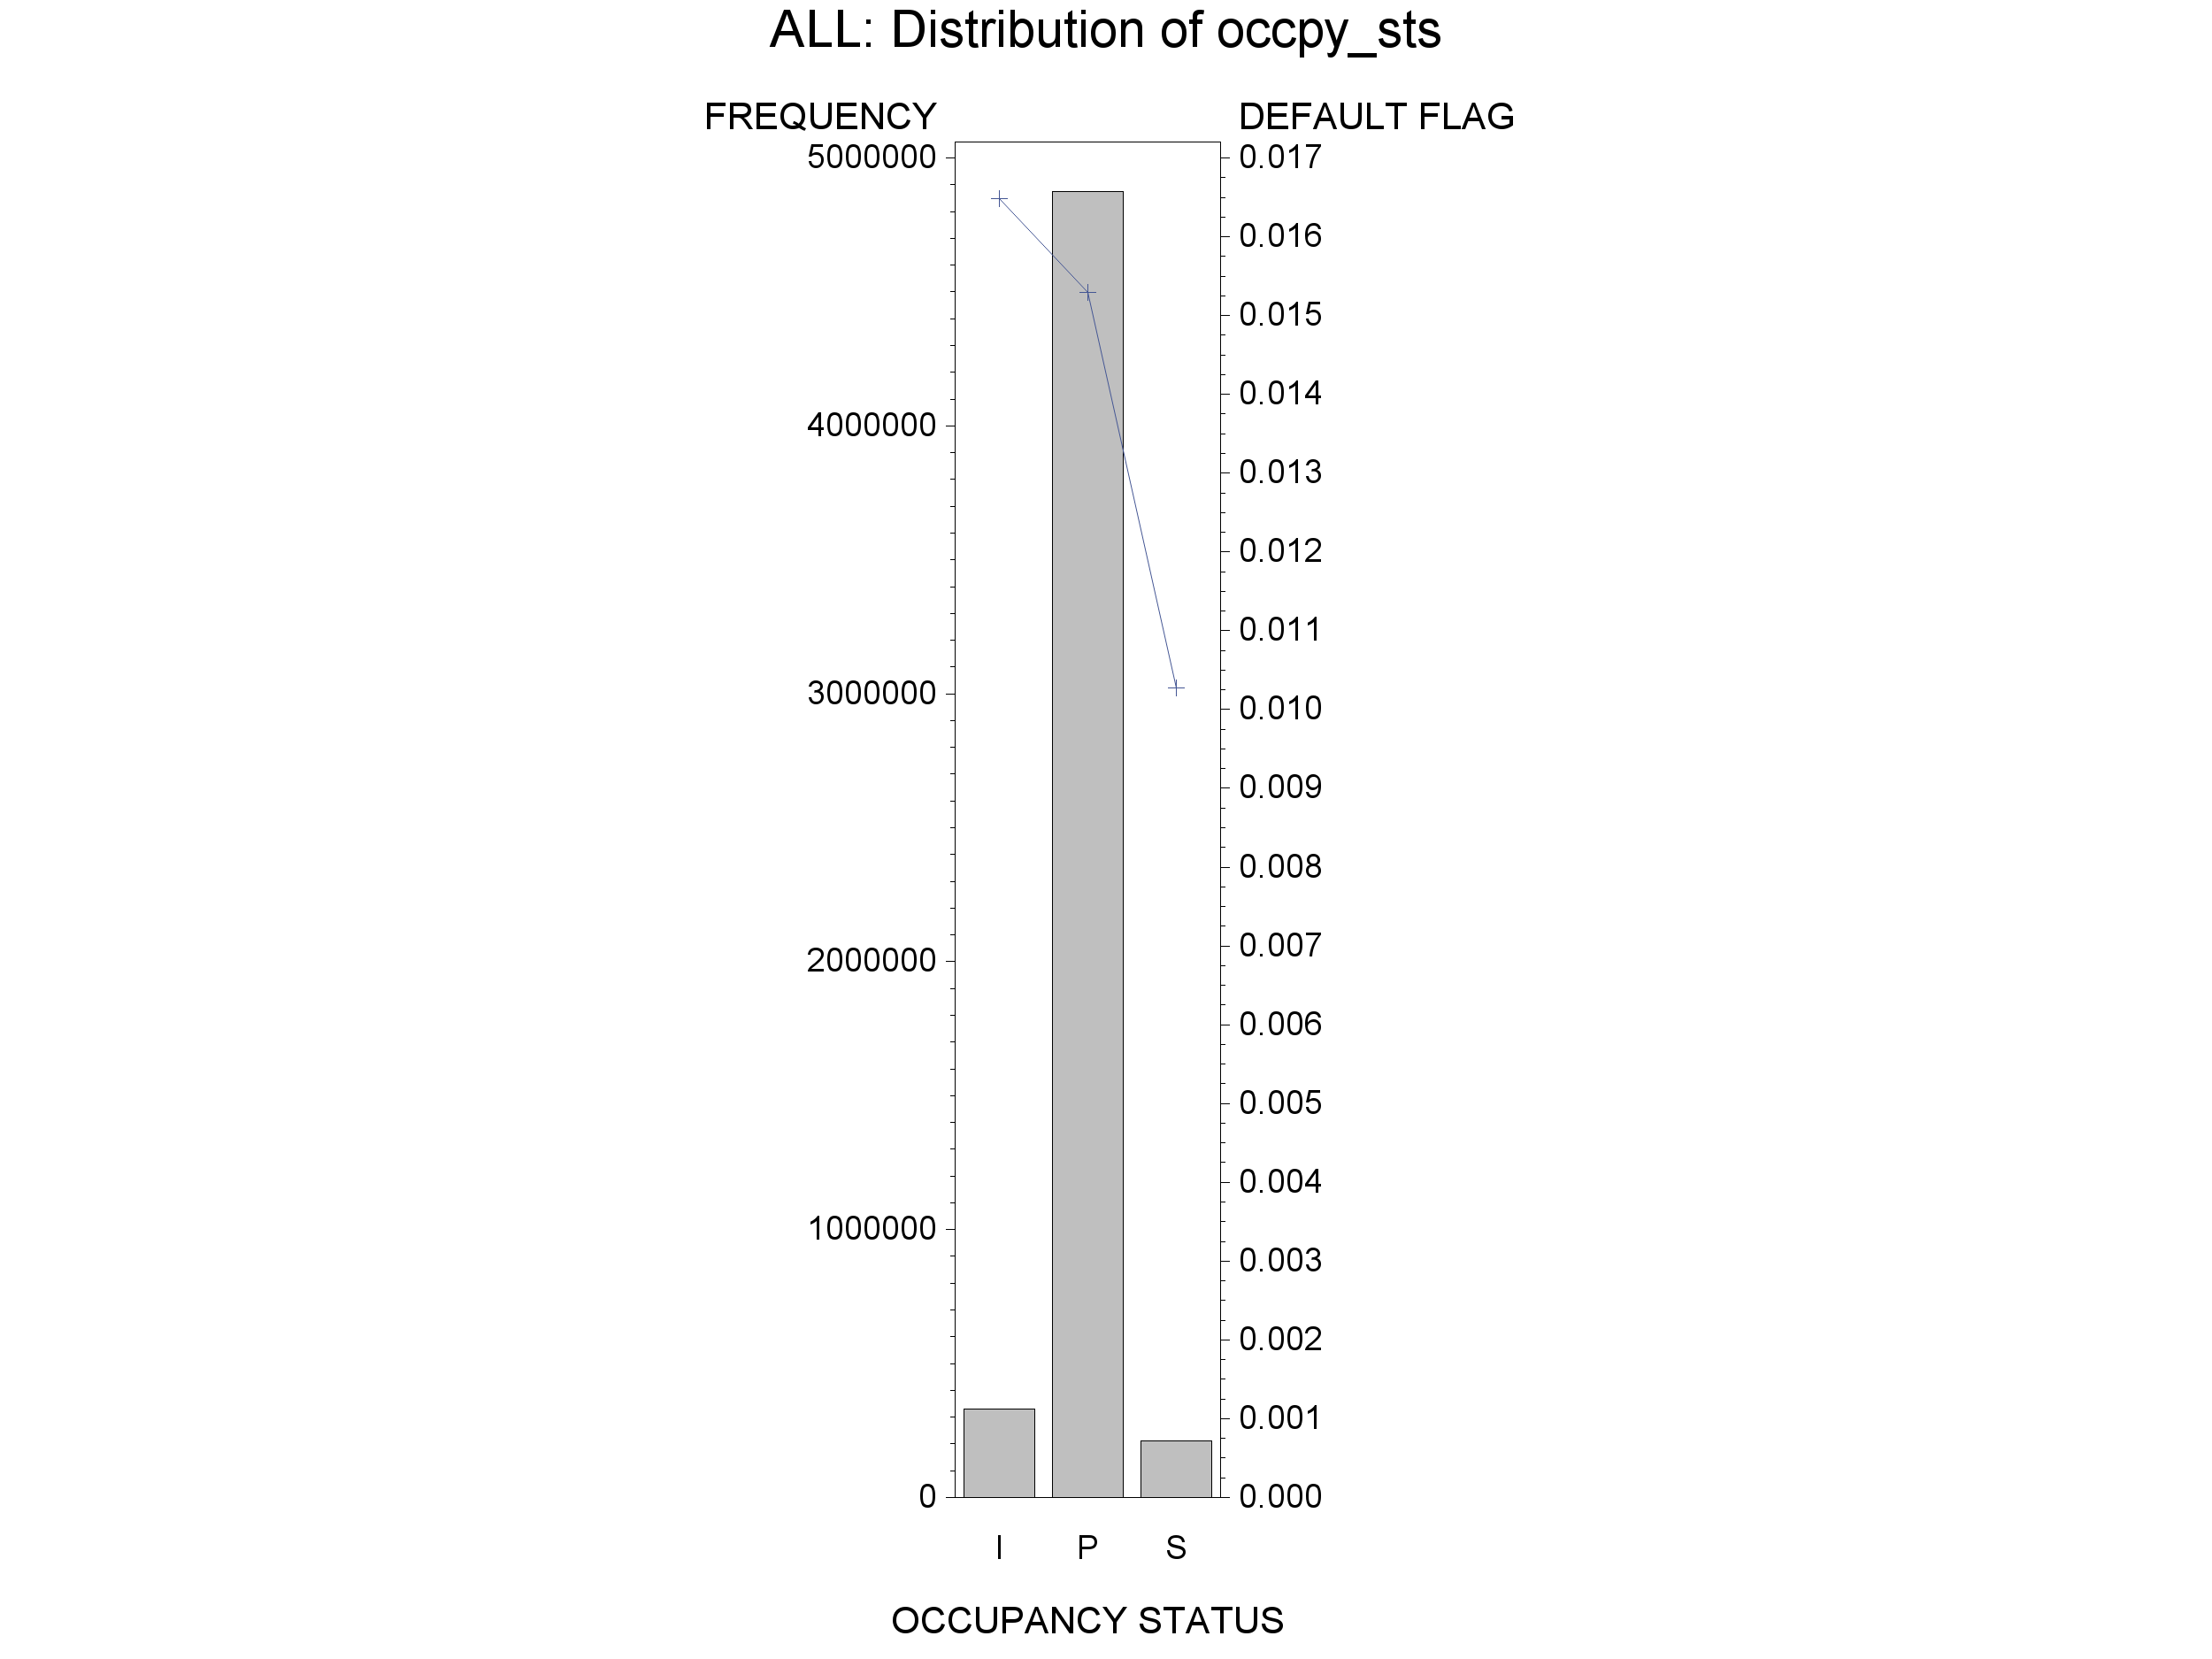
\includegraphics[width=0.9\textwidth]{./plot/Distribution/CAT_occpy_sts_DISTRIBUTION_ALL.png}
\end{minipage}%
\begin{minipage}{.5\textwidth}
	\centering
	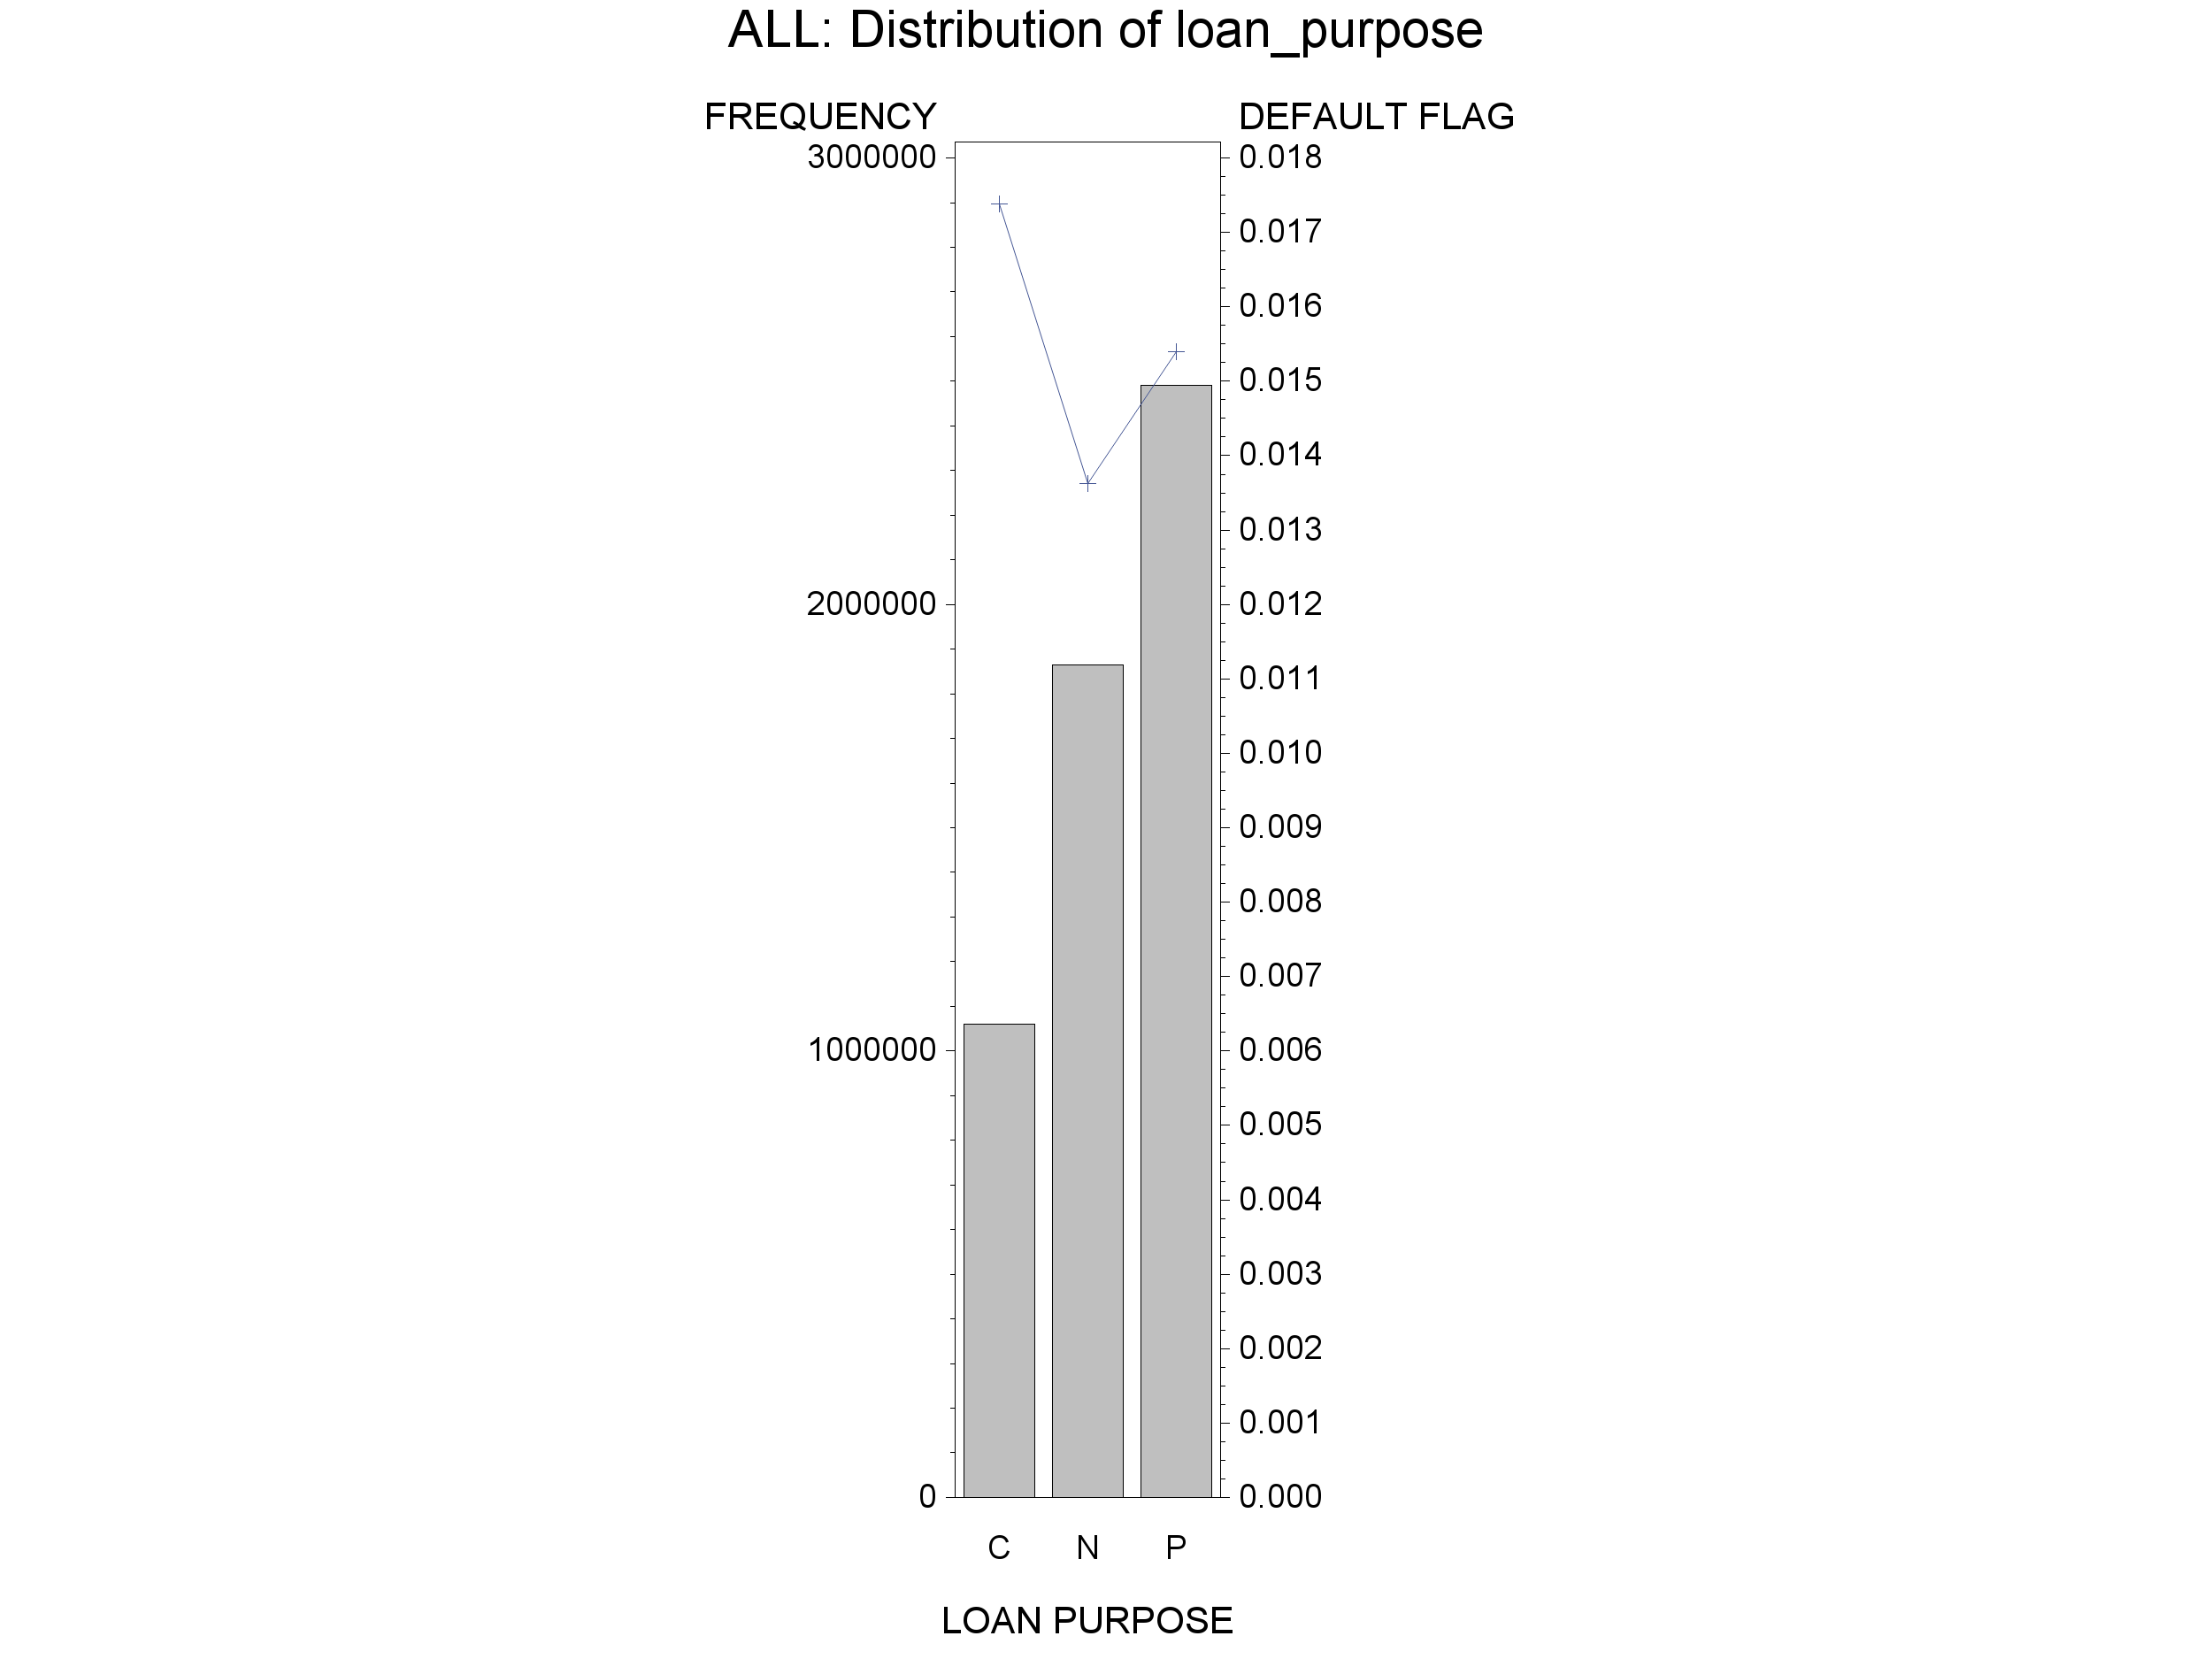
\includegraphics[width=0.9\textwidth]{./plot/Distribution/CAT_loan_purpose_DISTRIBUTION_ALL.png}
\end{minipage}
    \caption{Distribution and default rate of Occupancy and Loan Purpose}
\end{figure}

\begin{figure}[H]
\begin{minipage}{.5\textwidth}
	\centering
	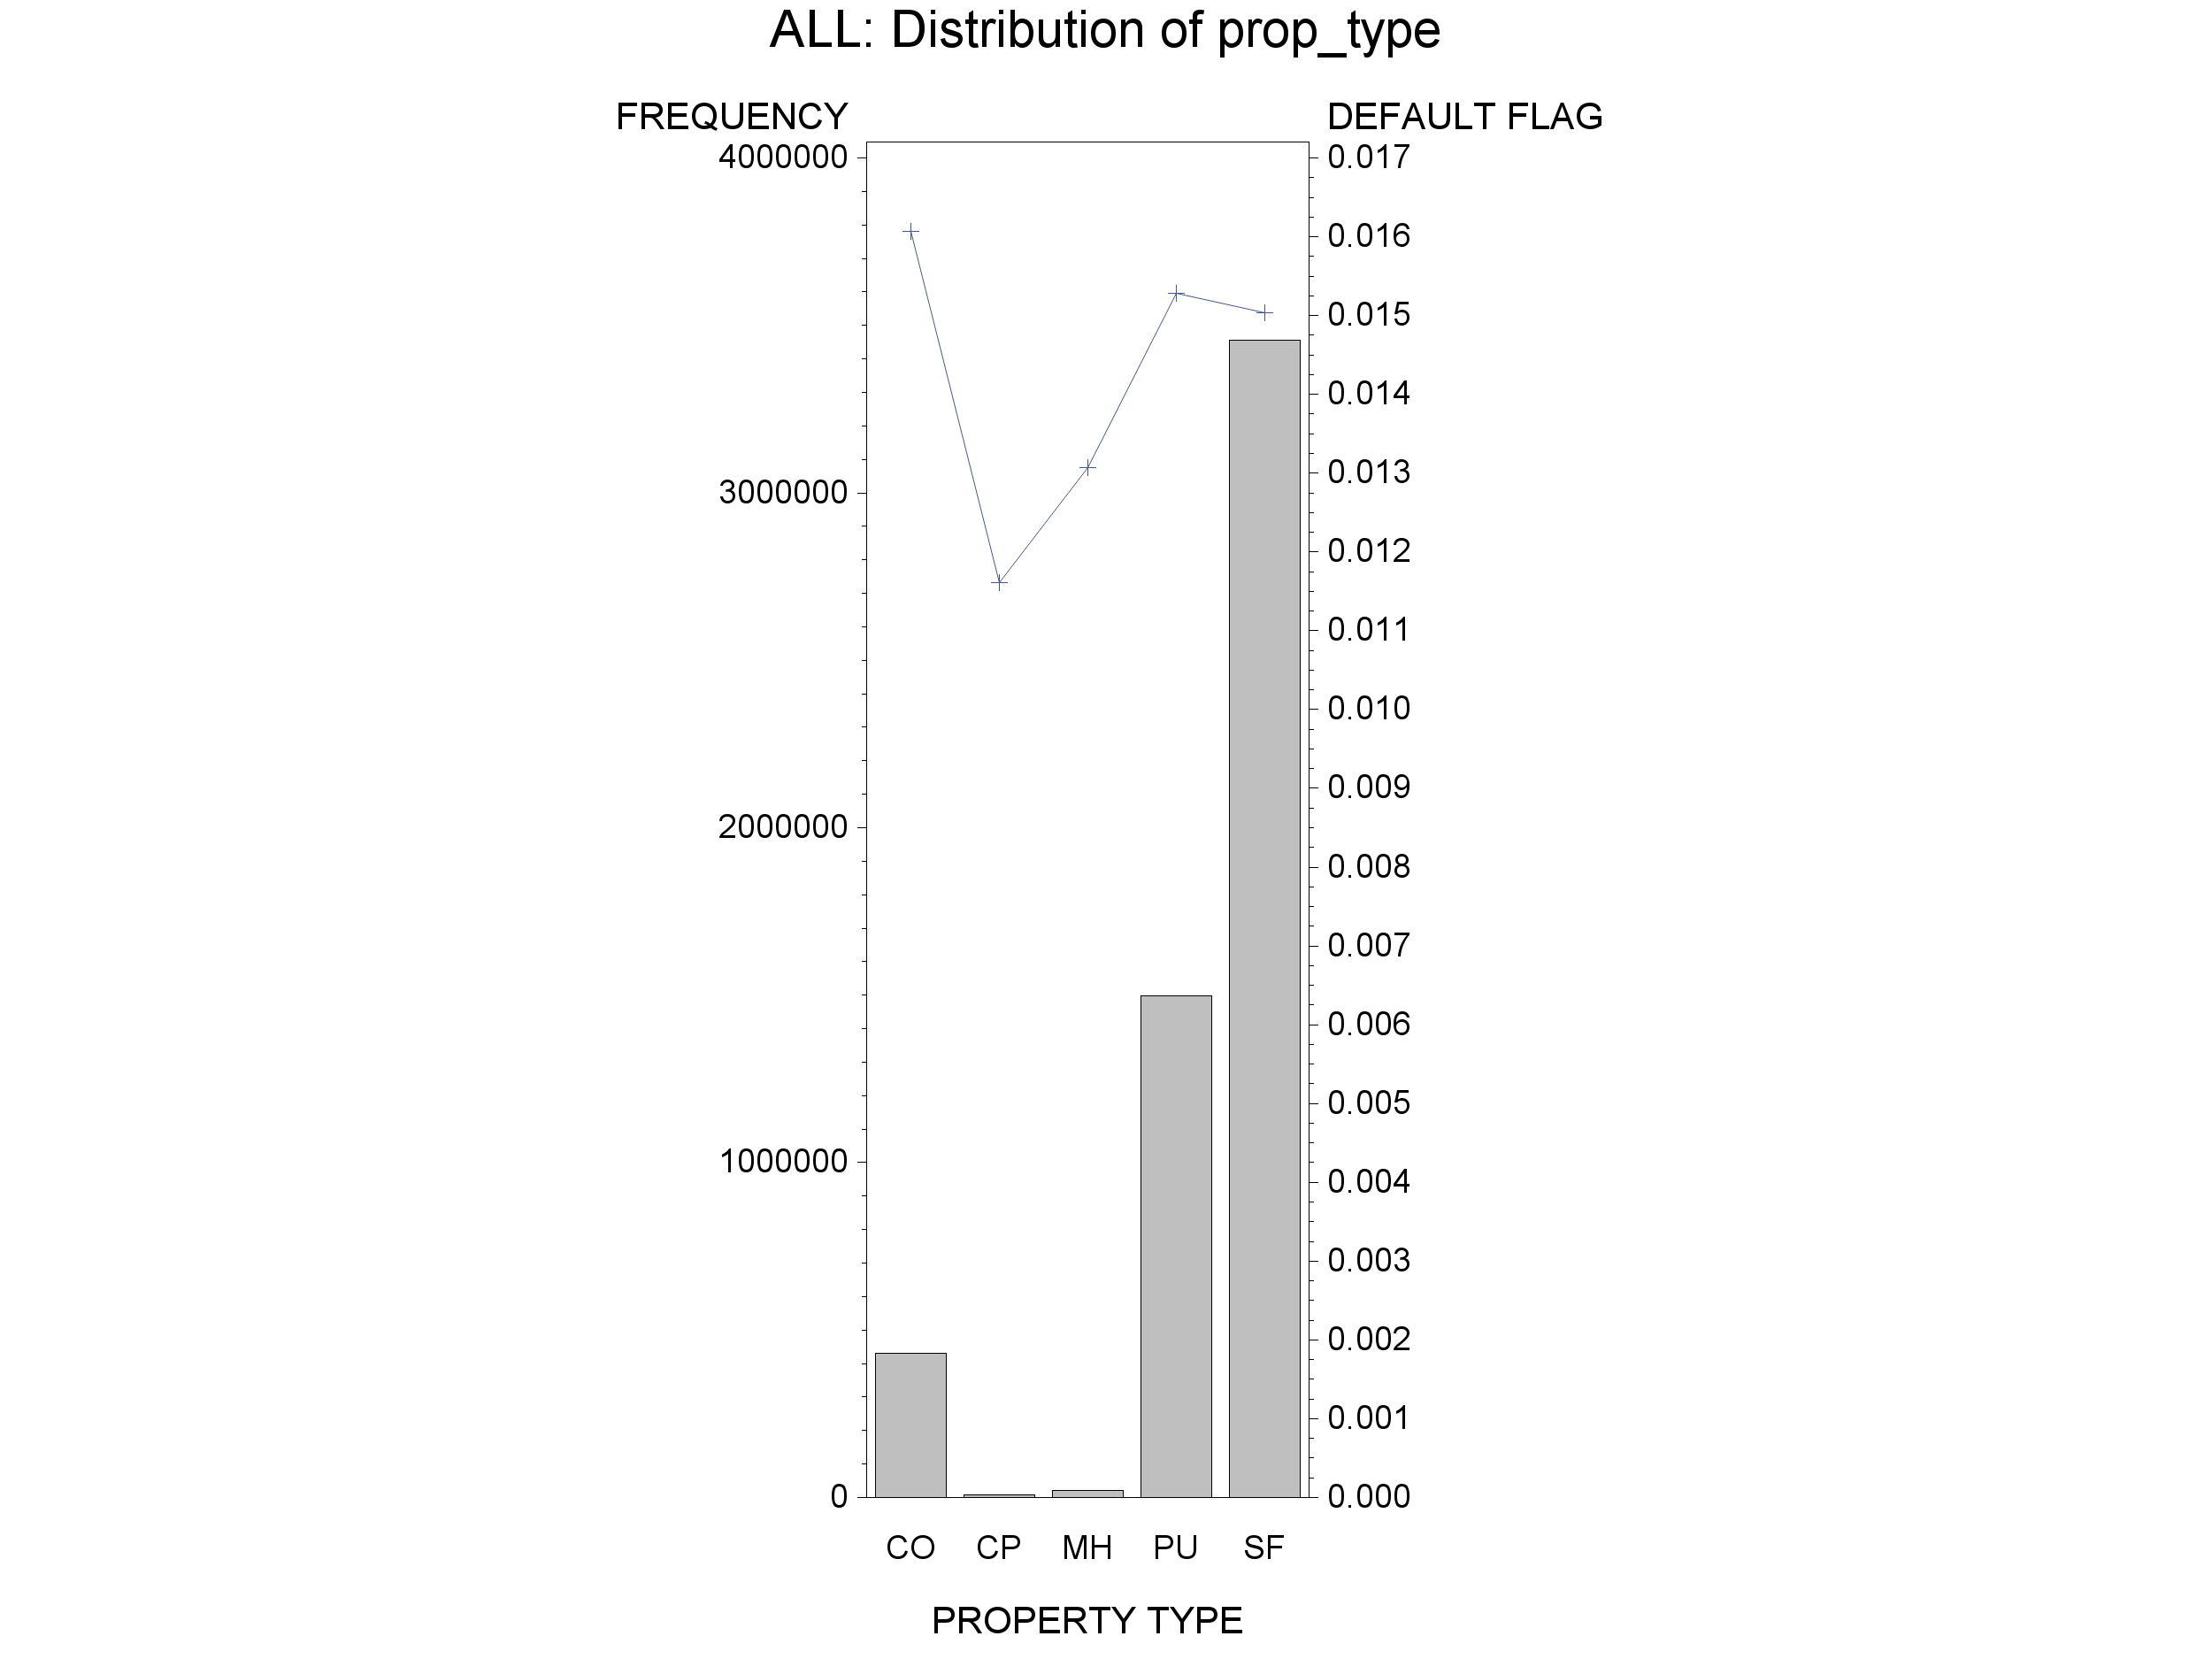
\includegraphics[width=0.9\textwidth]{./plot/Distribution/CAT_prop_type_DISTRIBUTION_ALL.png}
\end{minipage}%
\begin{minipage}{.5\textwidth}
	\centering
	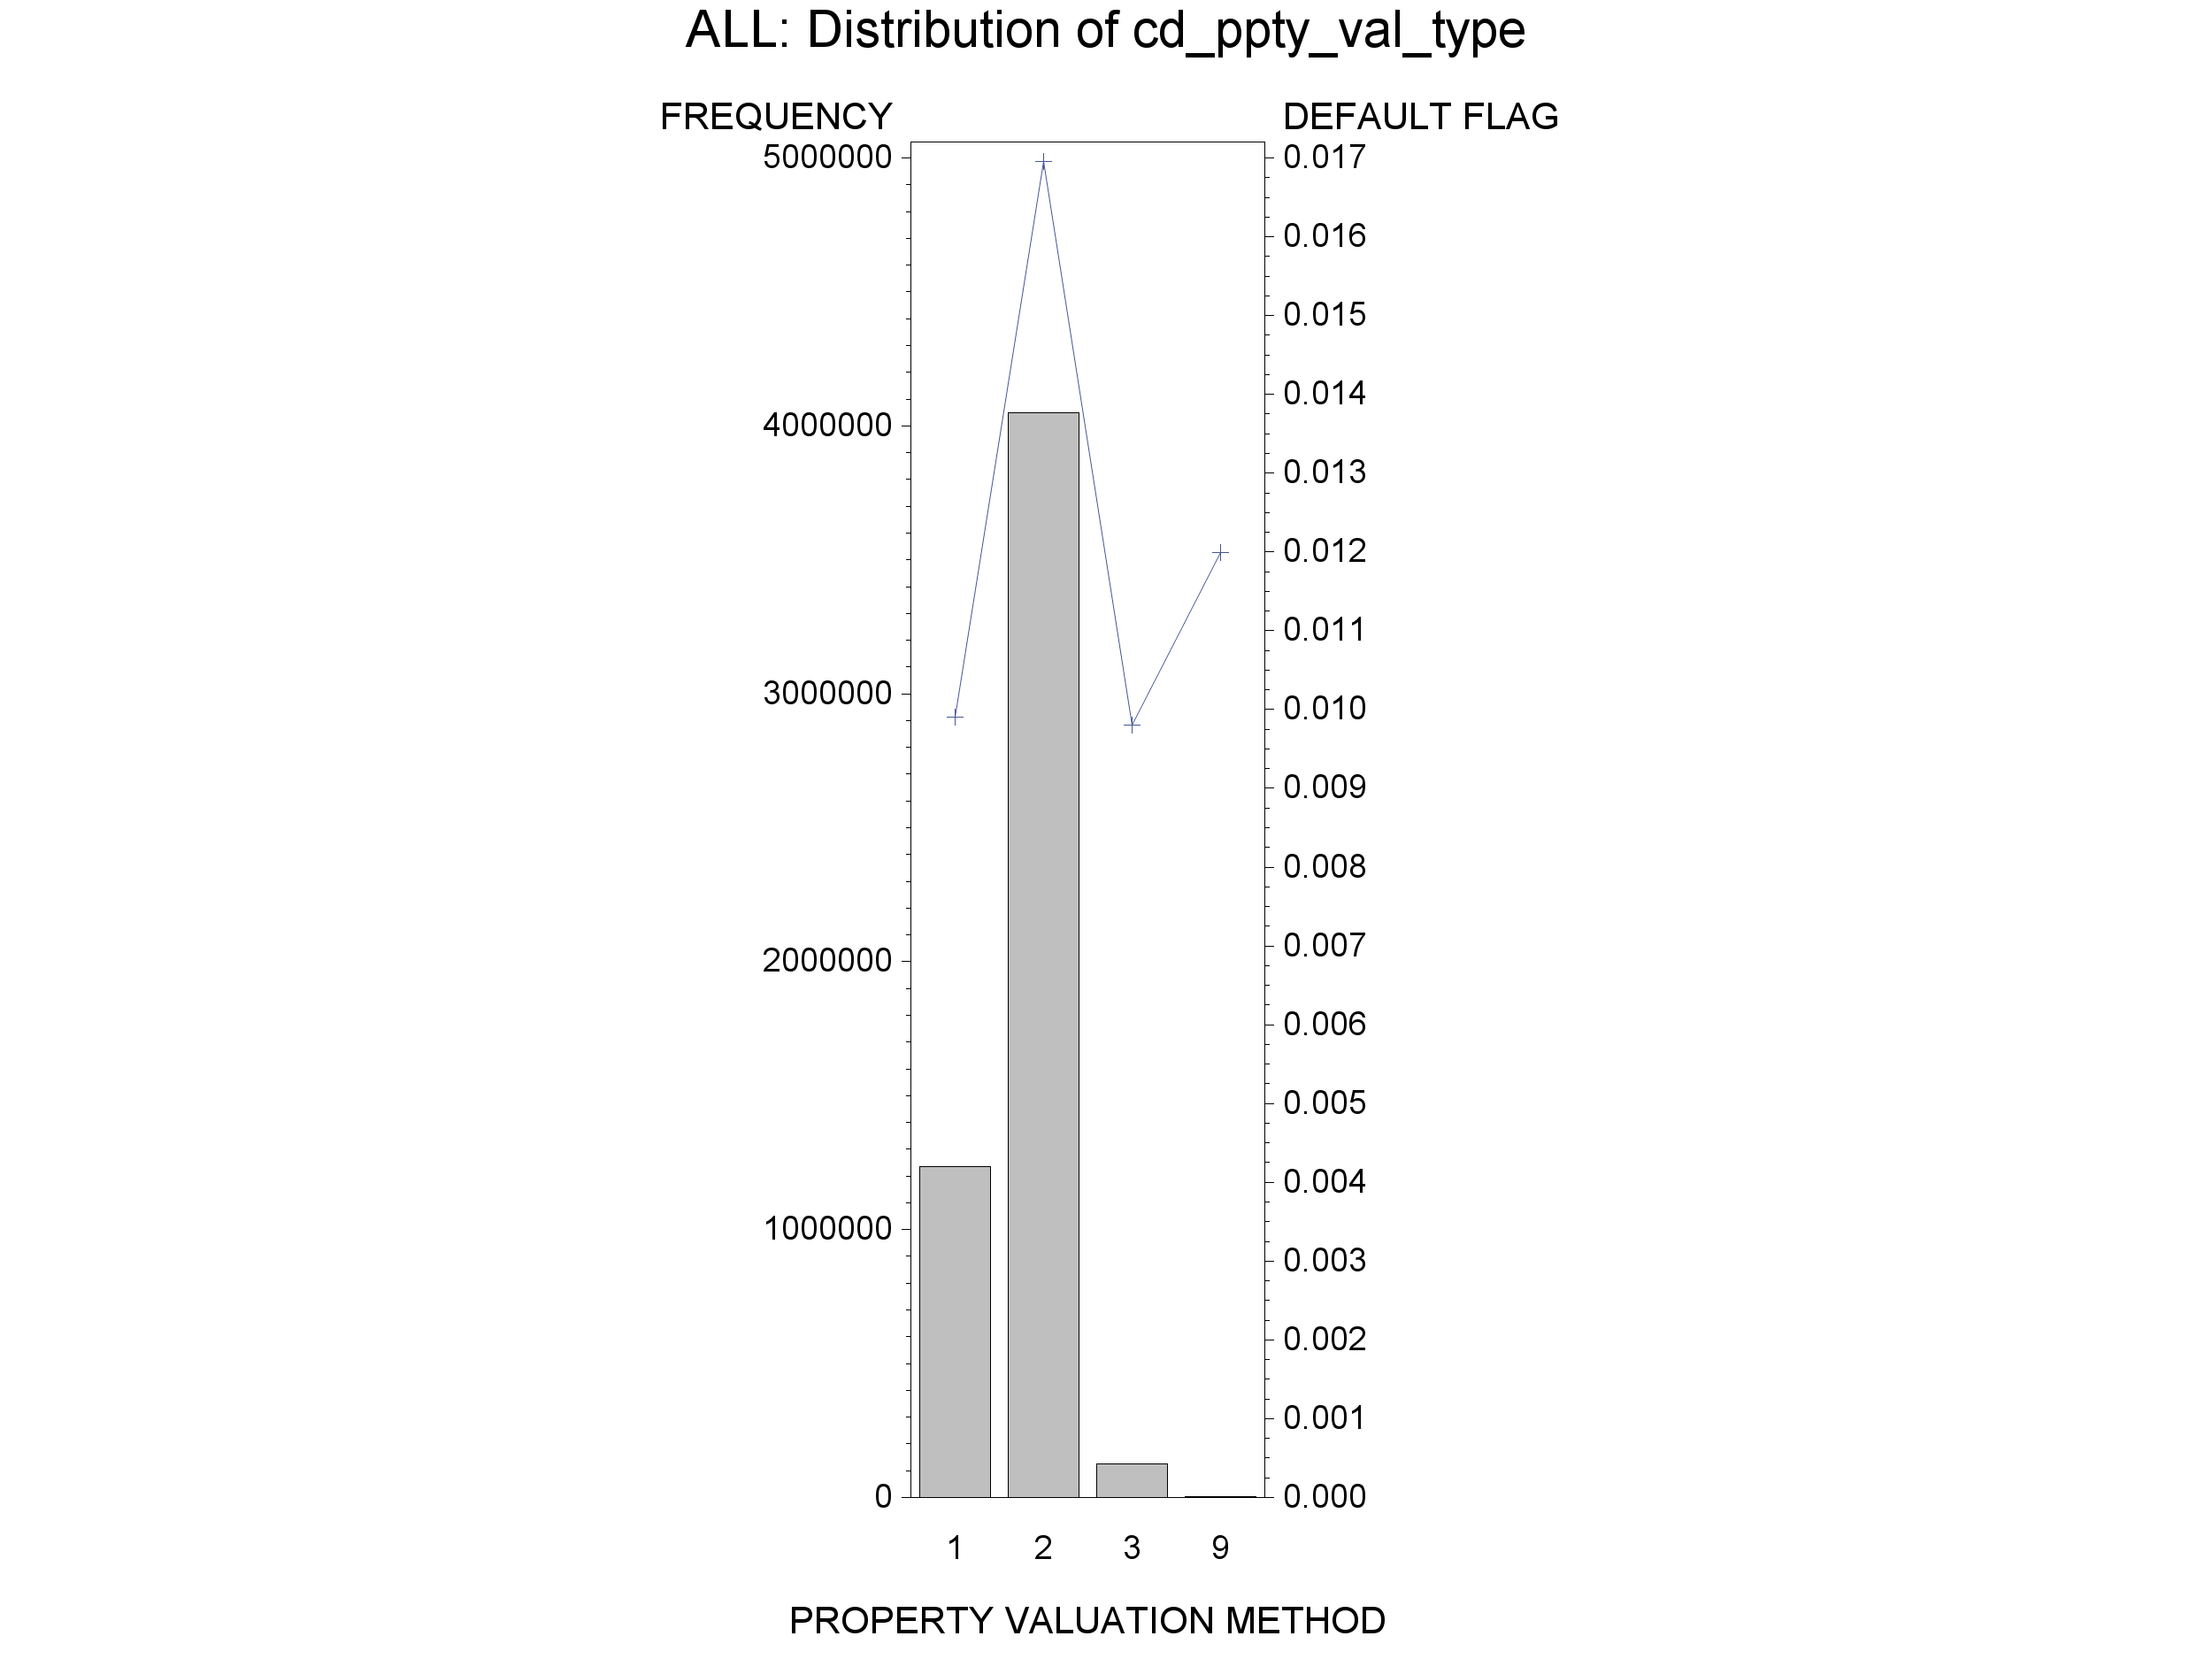
\includegraphics[width=0.9\textwidth]{./plot/Distribution/CAT_cd_ppty_val_type_DISTRIBUTION_ALL.png}
\end{minipage}
    \caption{Distribution and default rate of Prop Type and Valuation Method}
\end{figure}

\begin{figure}[H]
\begin{minipage}{.5\textwidth}
	\centering
	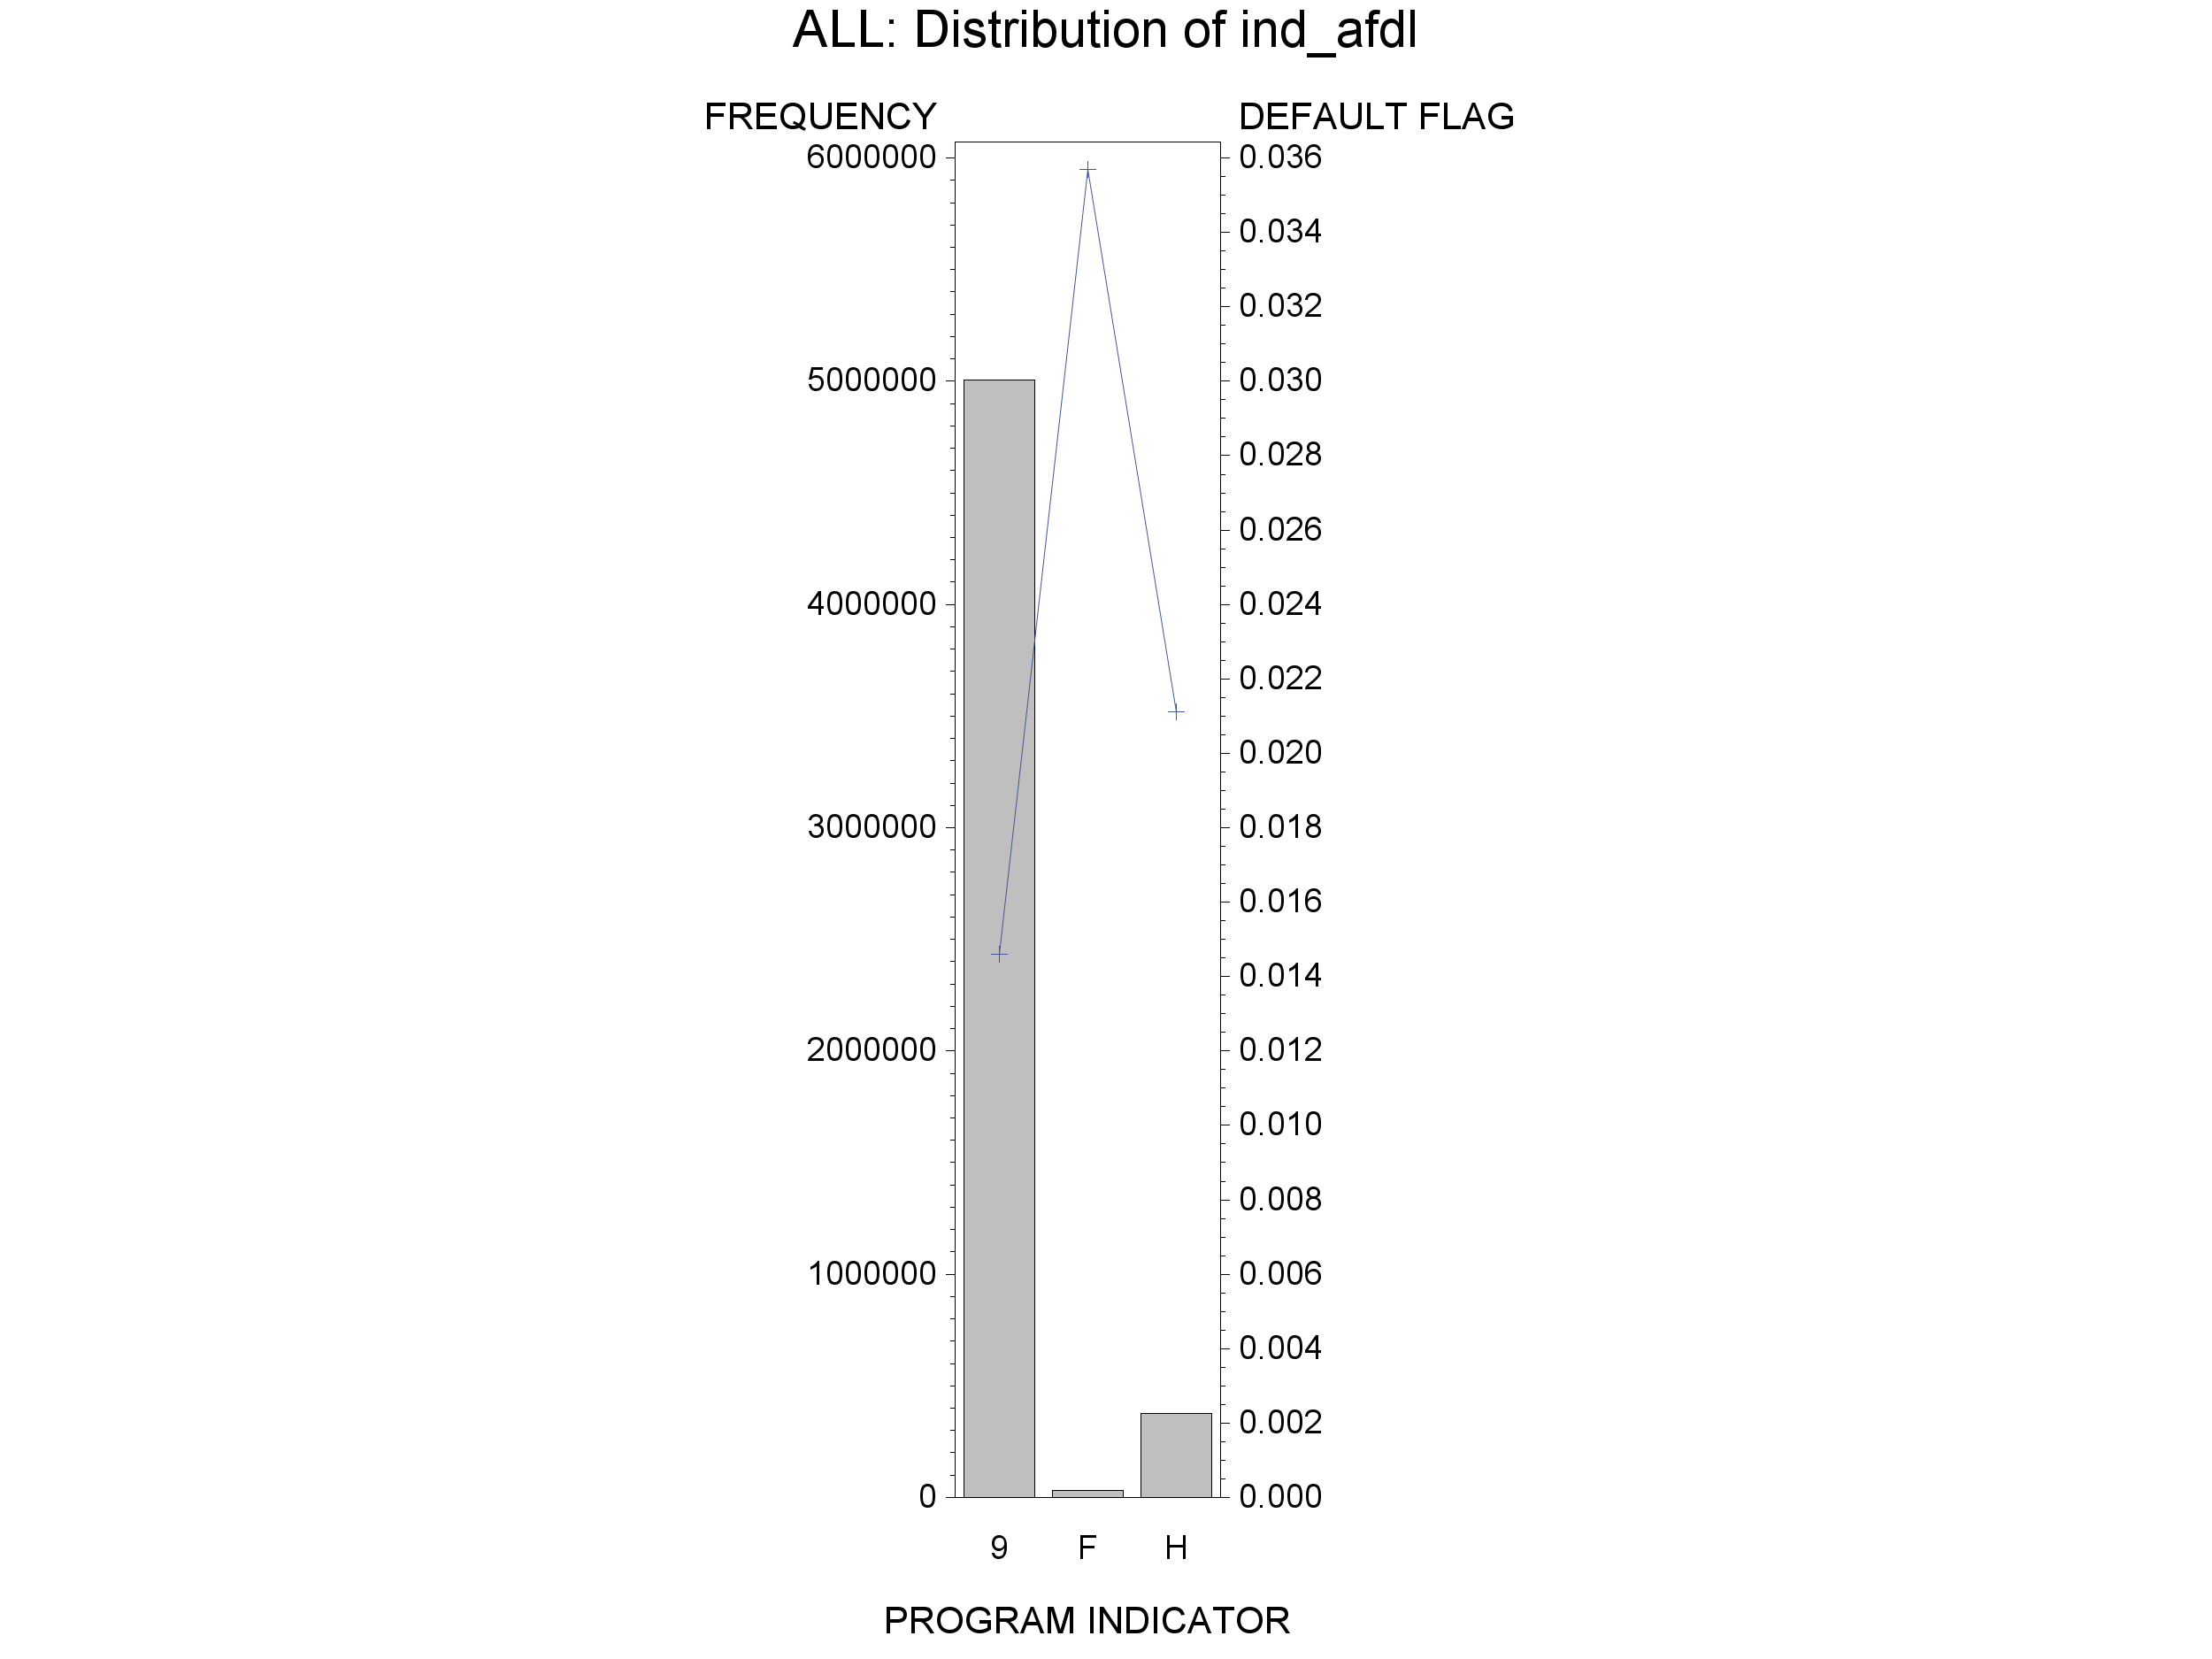
\includegraphics[width=0.9\textwidth]{./plot/Distribution/CAT_ind_afdl_DISTRIBUTION_ALL.png}
\end{minipage}%
\begin{minipage}{.5\textwidth}
	\centering
	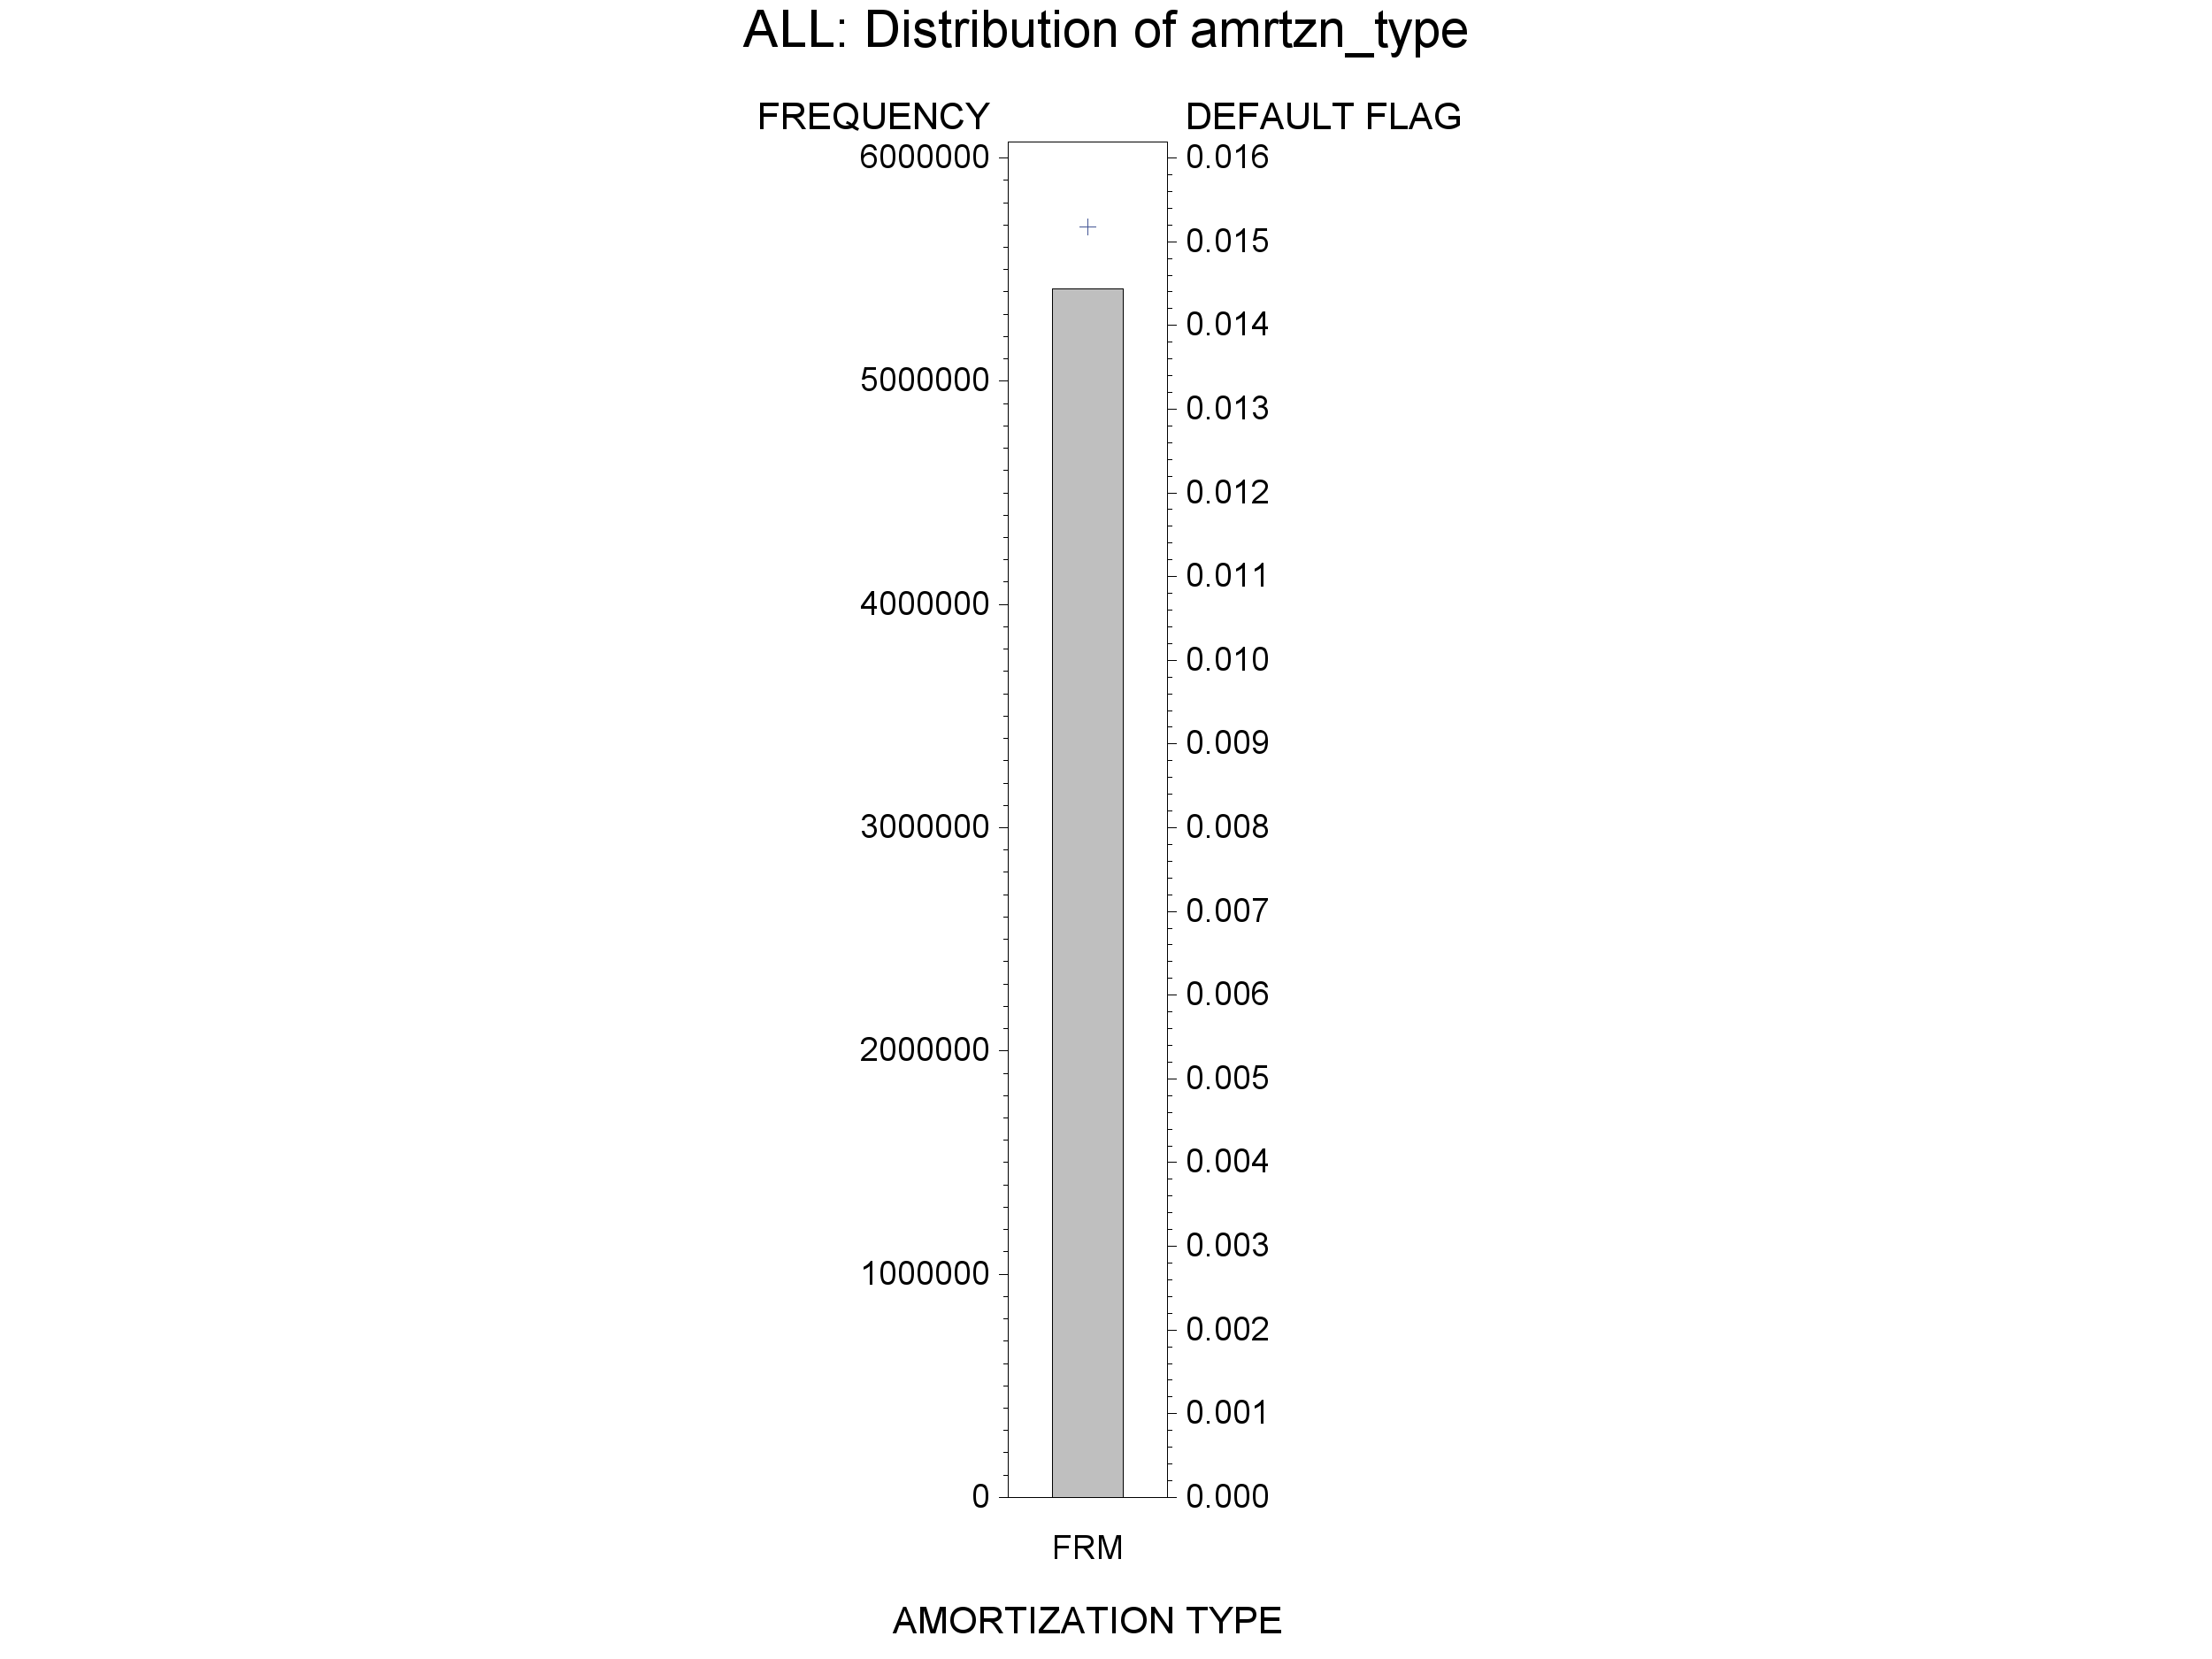
\includegraphics[width=0.9\textwidth]{./plot/Distribution/CAT_amrtzn_type_DISTRIBUTION_ALL.png}
\end{minipage}
    \caption{Distribution and default rate of Prog Flag and Amort Type}
\end{figure}

\begin{figure}[H]
\begin{minipage}{.5\textwidth}
	\centering
	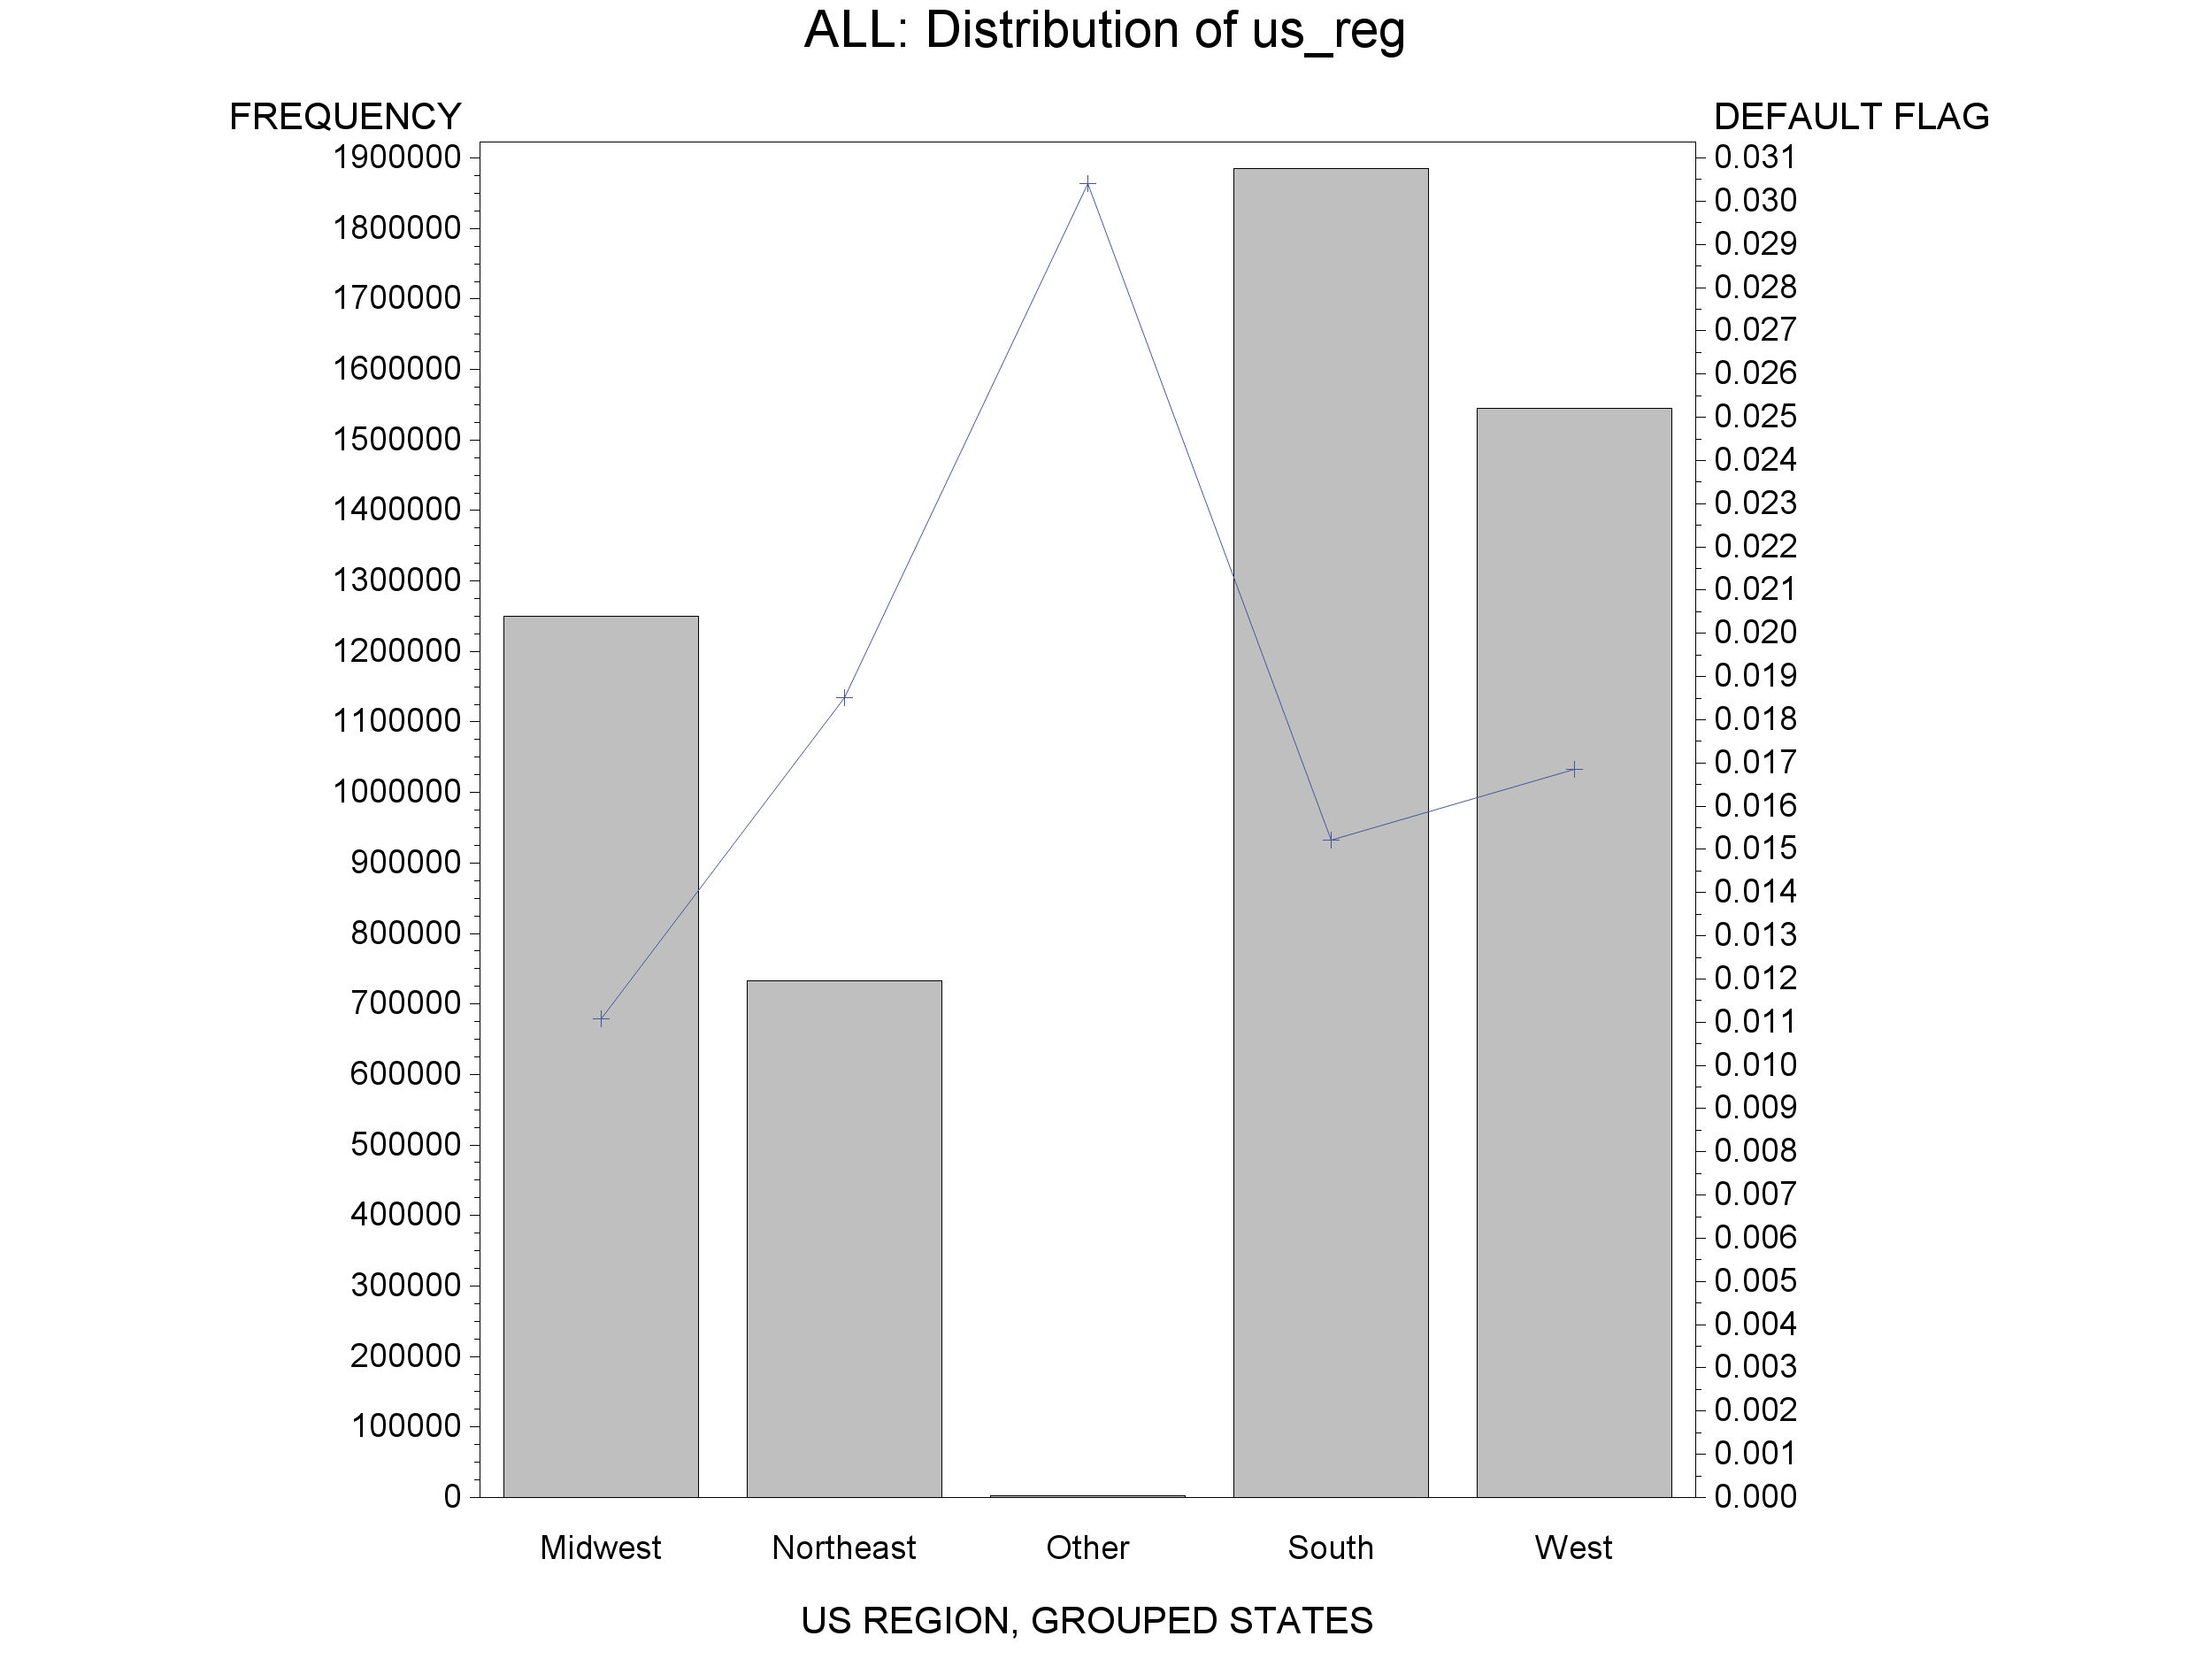
\includegraphics[width=0.9\textwidth]{./plot/Distribution/Main/RE_CAT_us_reg_DISTRIBUTION_ALL.png}
\end{minipage}%
\begin{minipage}{.5\textwidth}
	\centering
	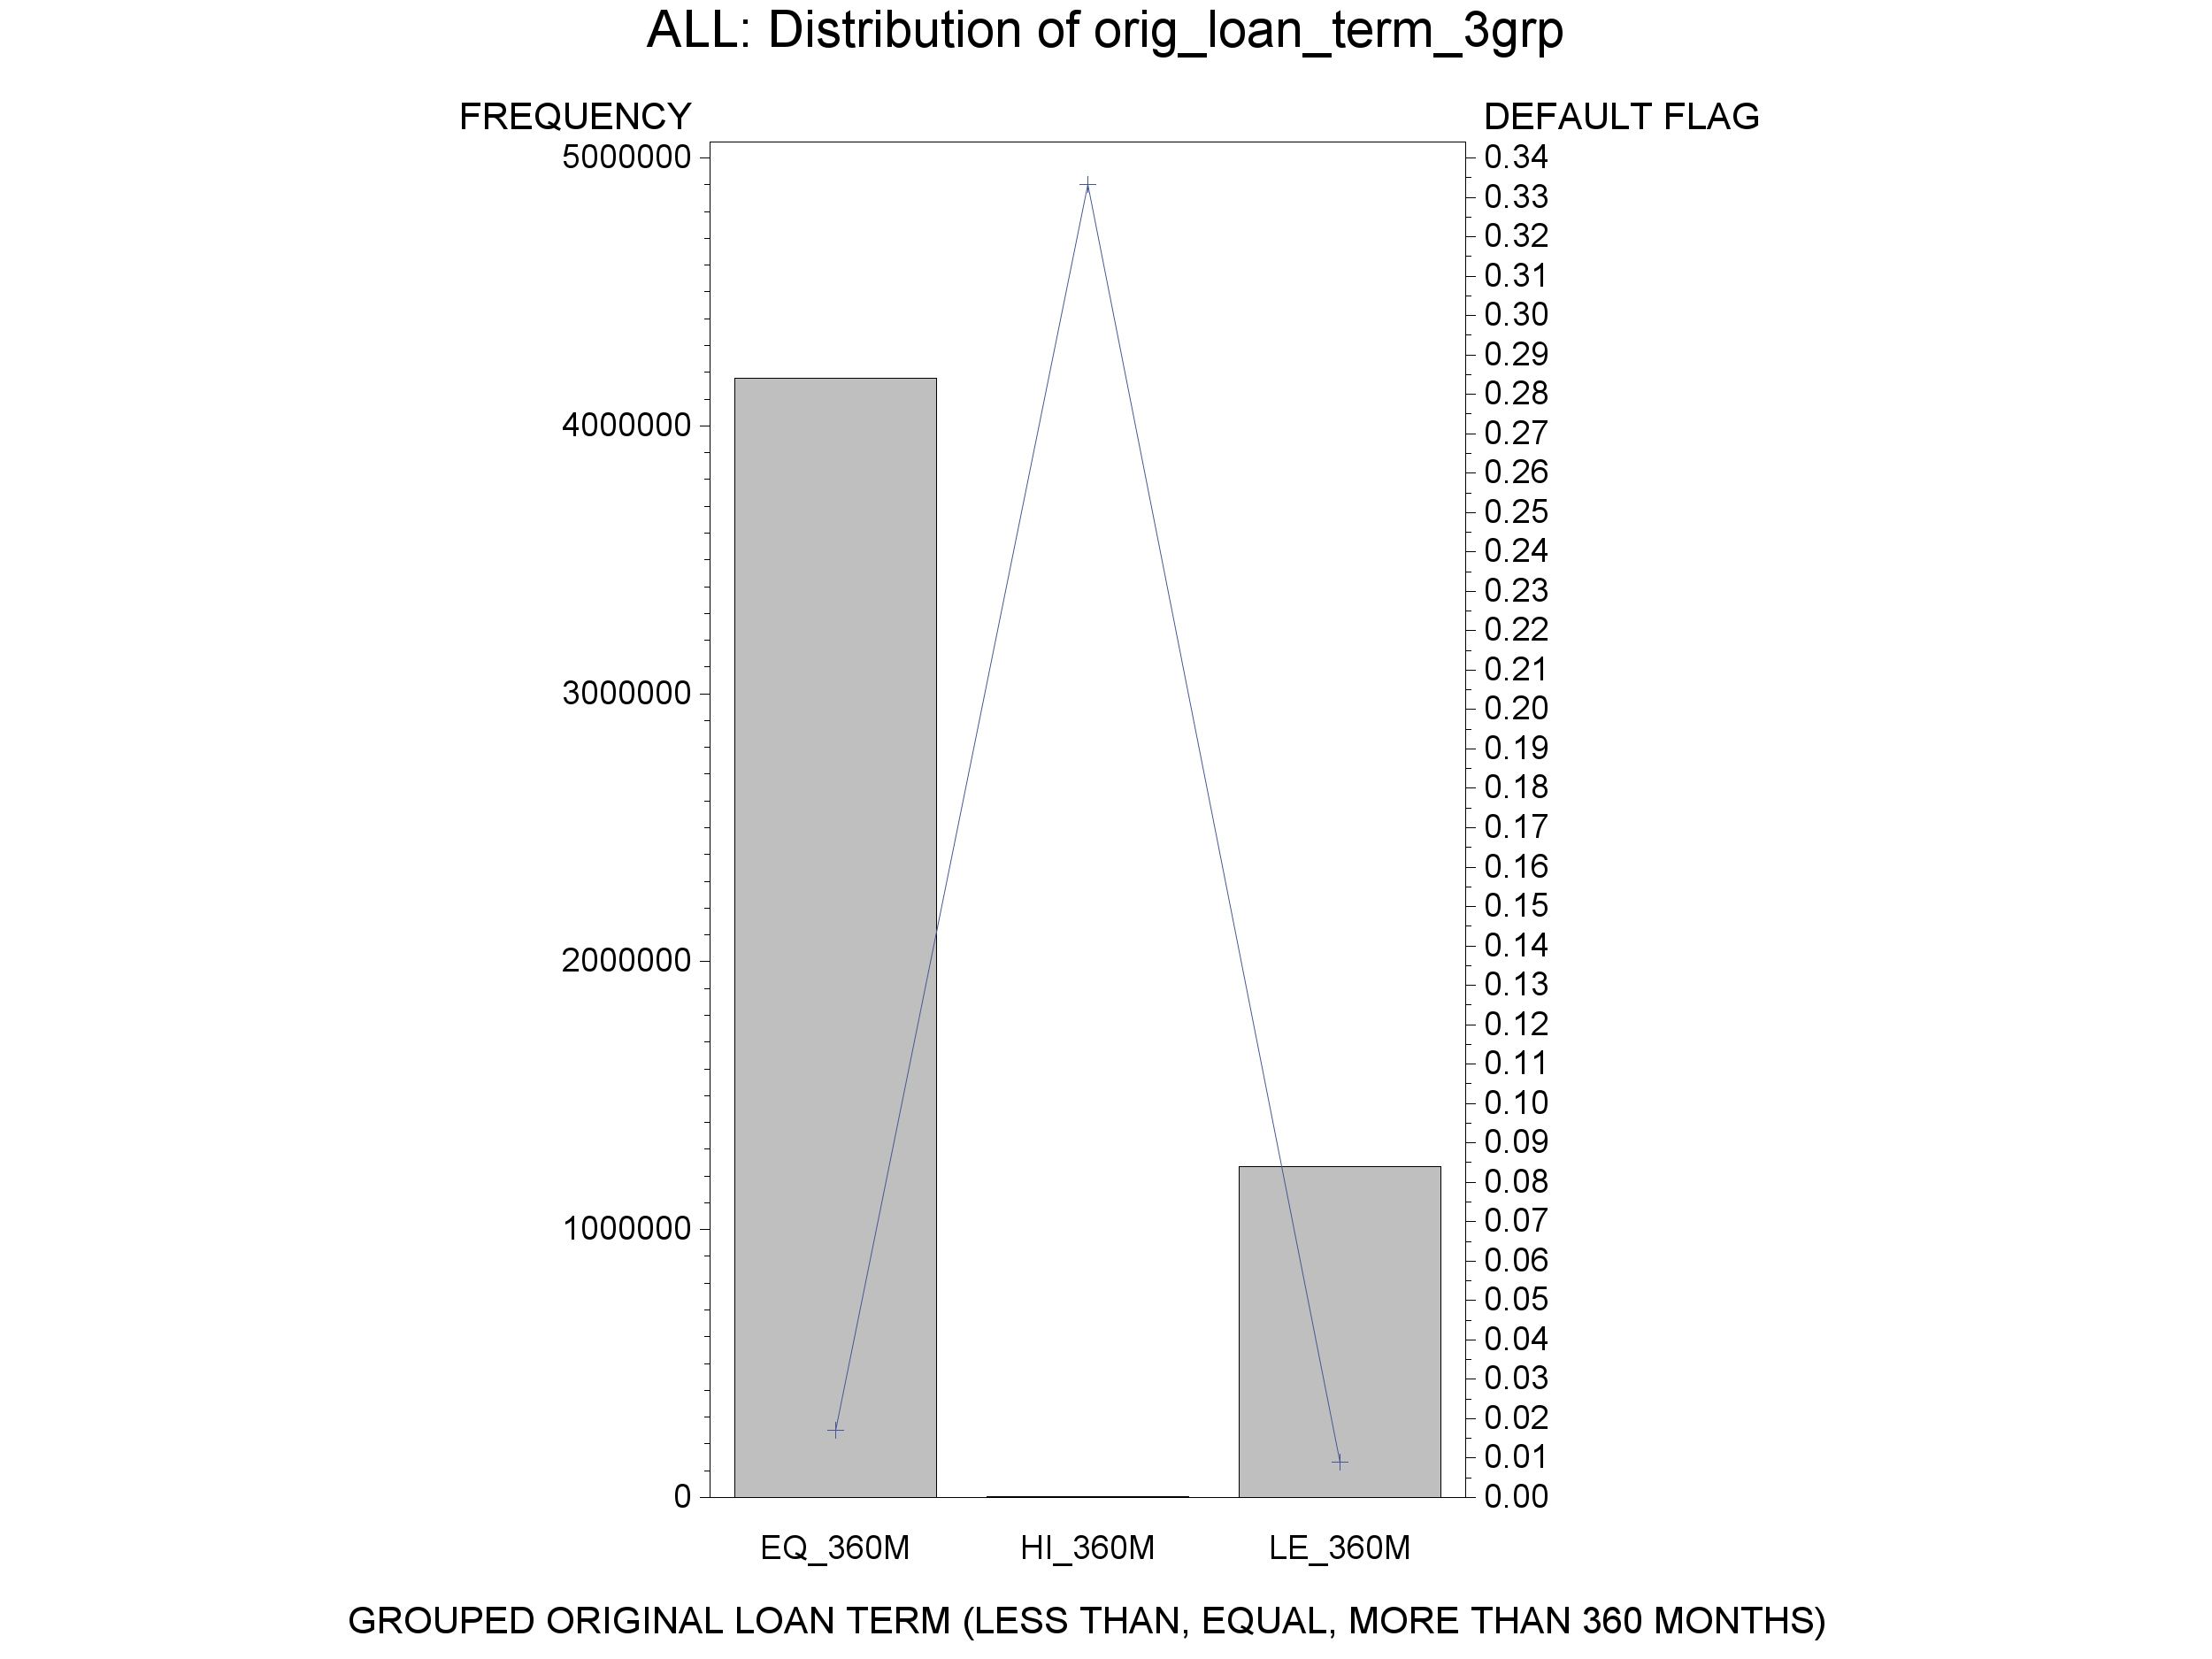
\includegraphics[width=0.9\textwidth]{./plot/Distribution/CAT_orig_loan_term_3grp_DISTRIBUTION_ALL.png}
\end{minipage}
    \caption{Distribution and default rate of US region and Loan Term (grouped)}
\end{figure}

\begin{figure}[H]
	\centering
	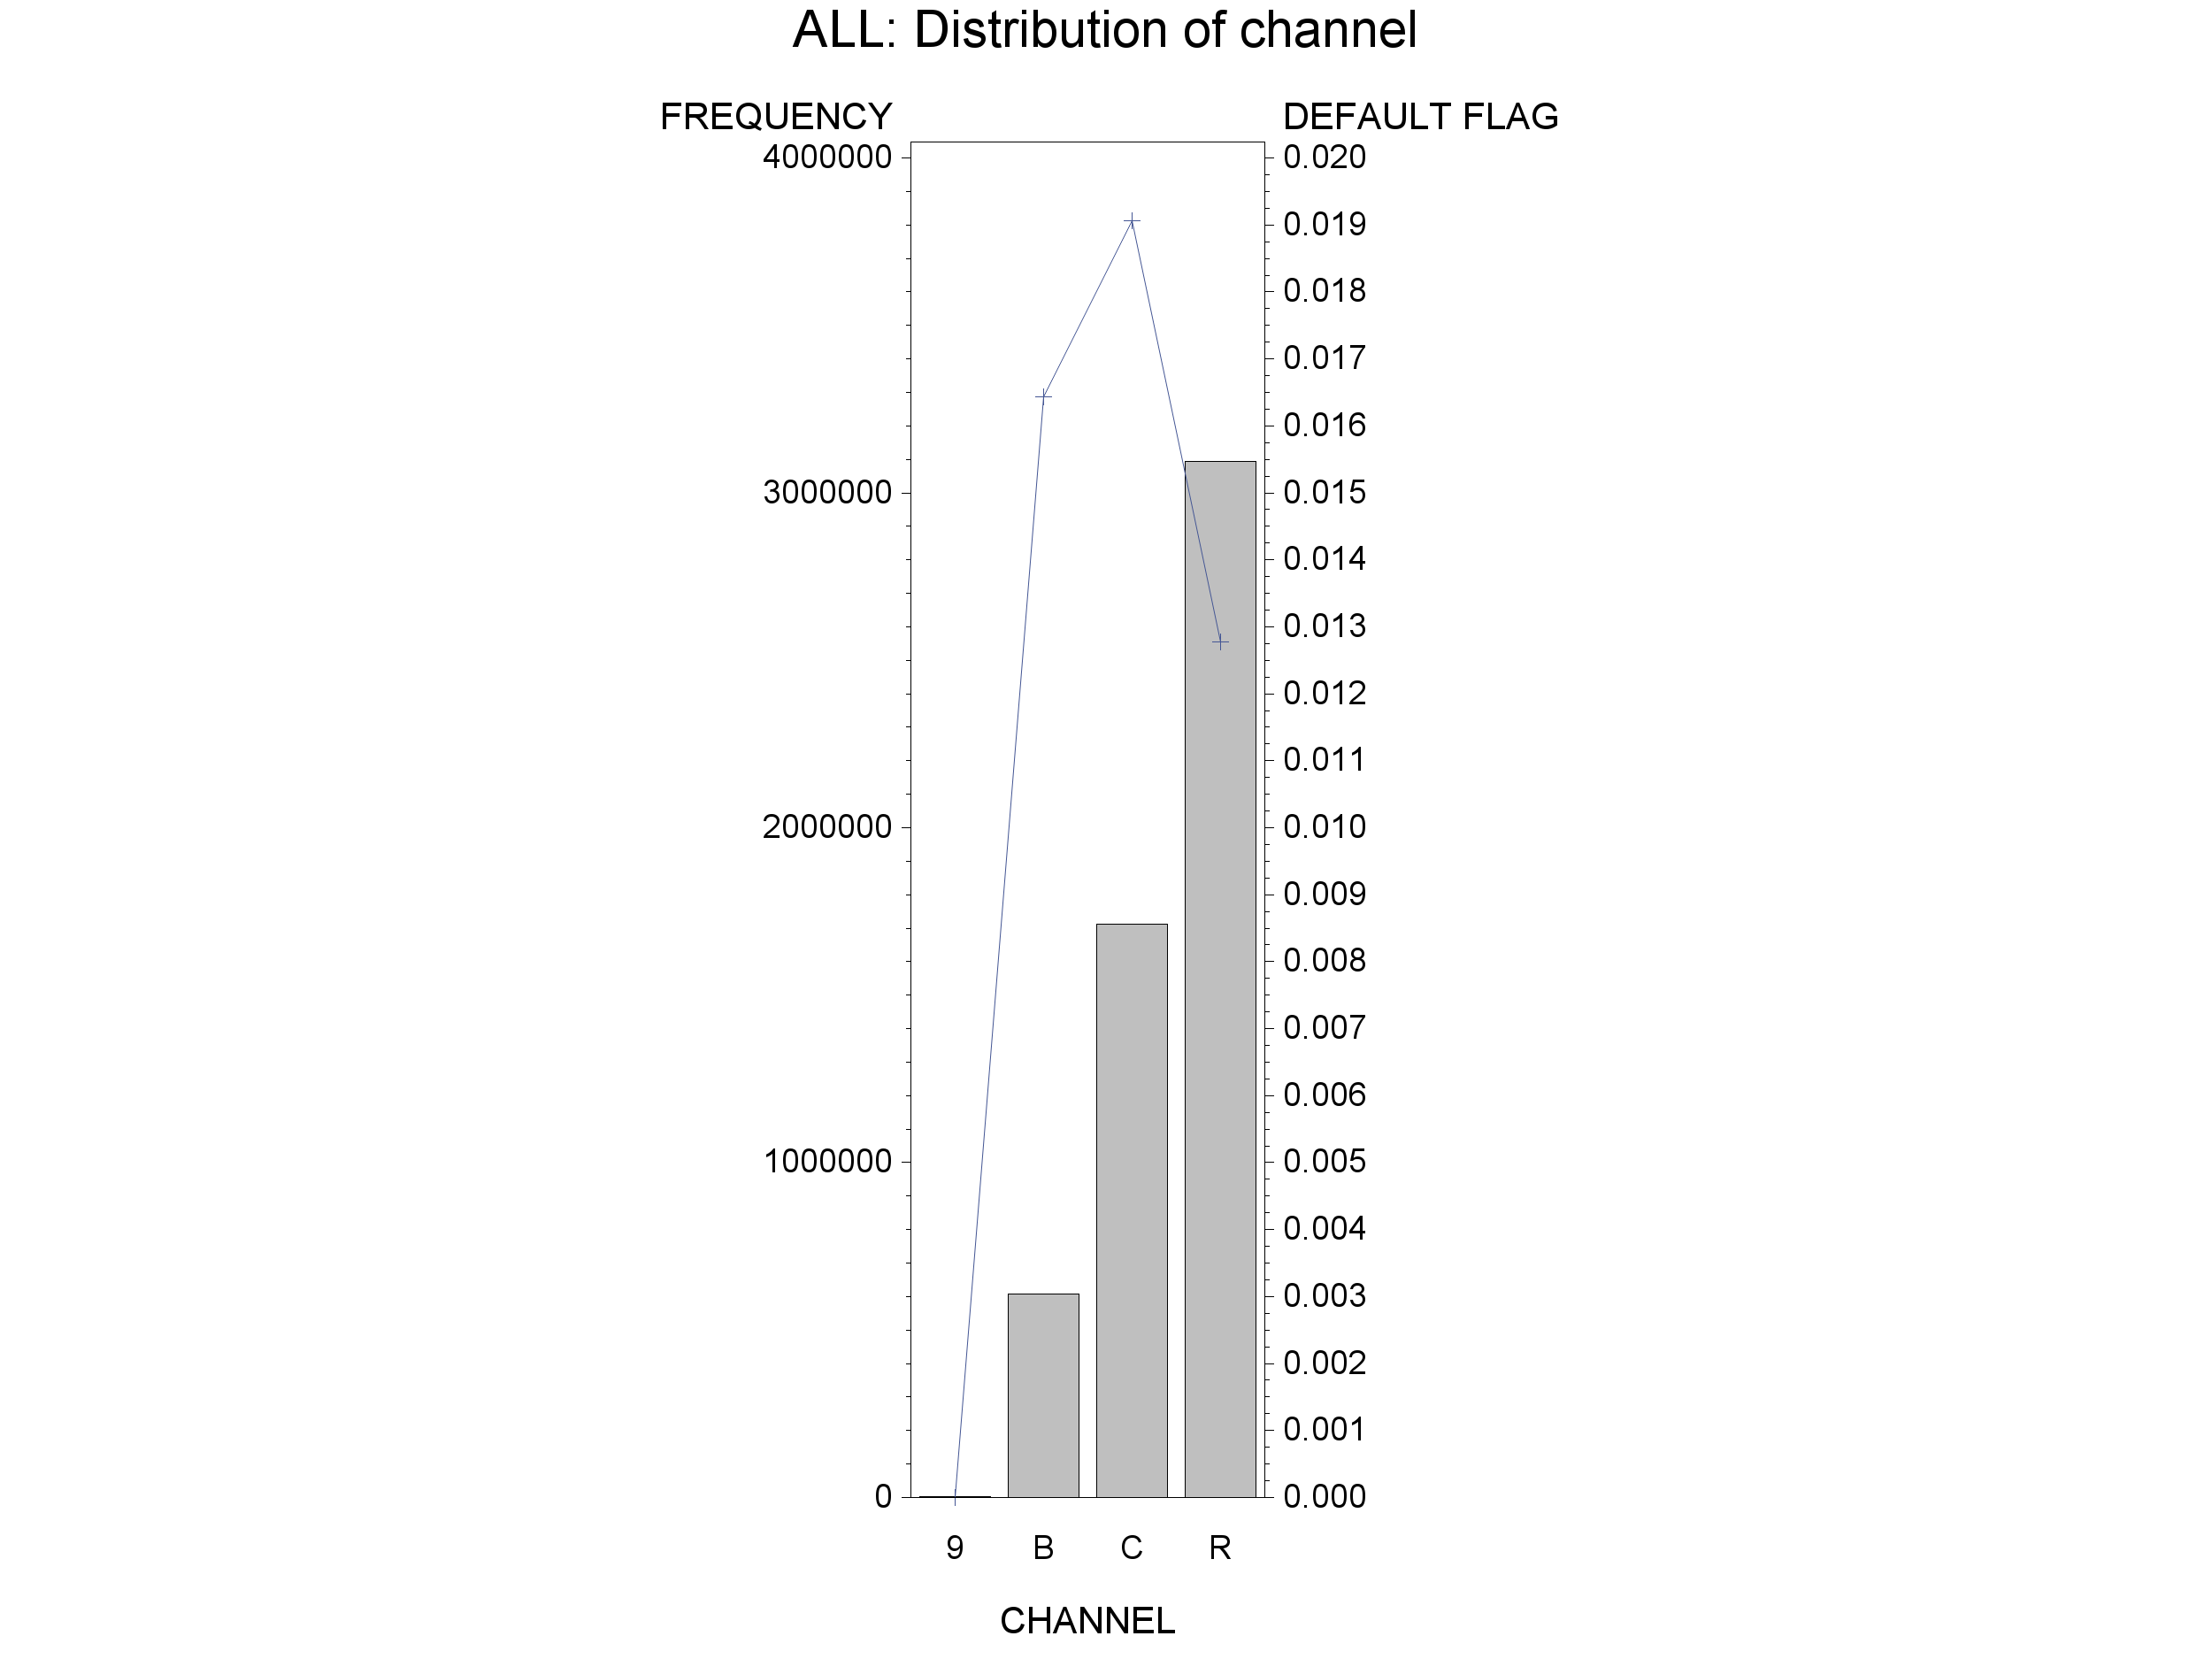
\includegraphics[width=0.5\textwidth]{./plot/Distribution/Main/RE_CAT_channel_DISTRIBUTION_ALL.png}
    \caption{Distribution and default rate of Channel}
\end{figure}

\subsection{Indicator variables}

\begin{figure}[H]
\begin{minipage}{.5\textwidth}
	\centering
	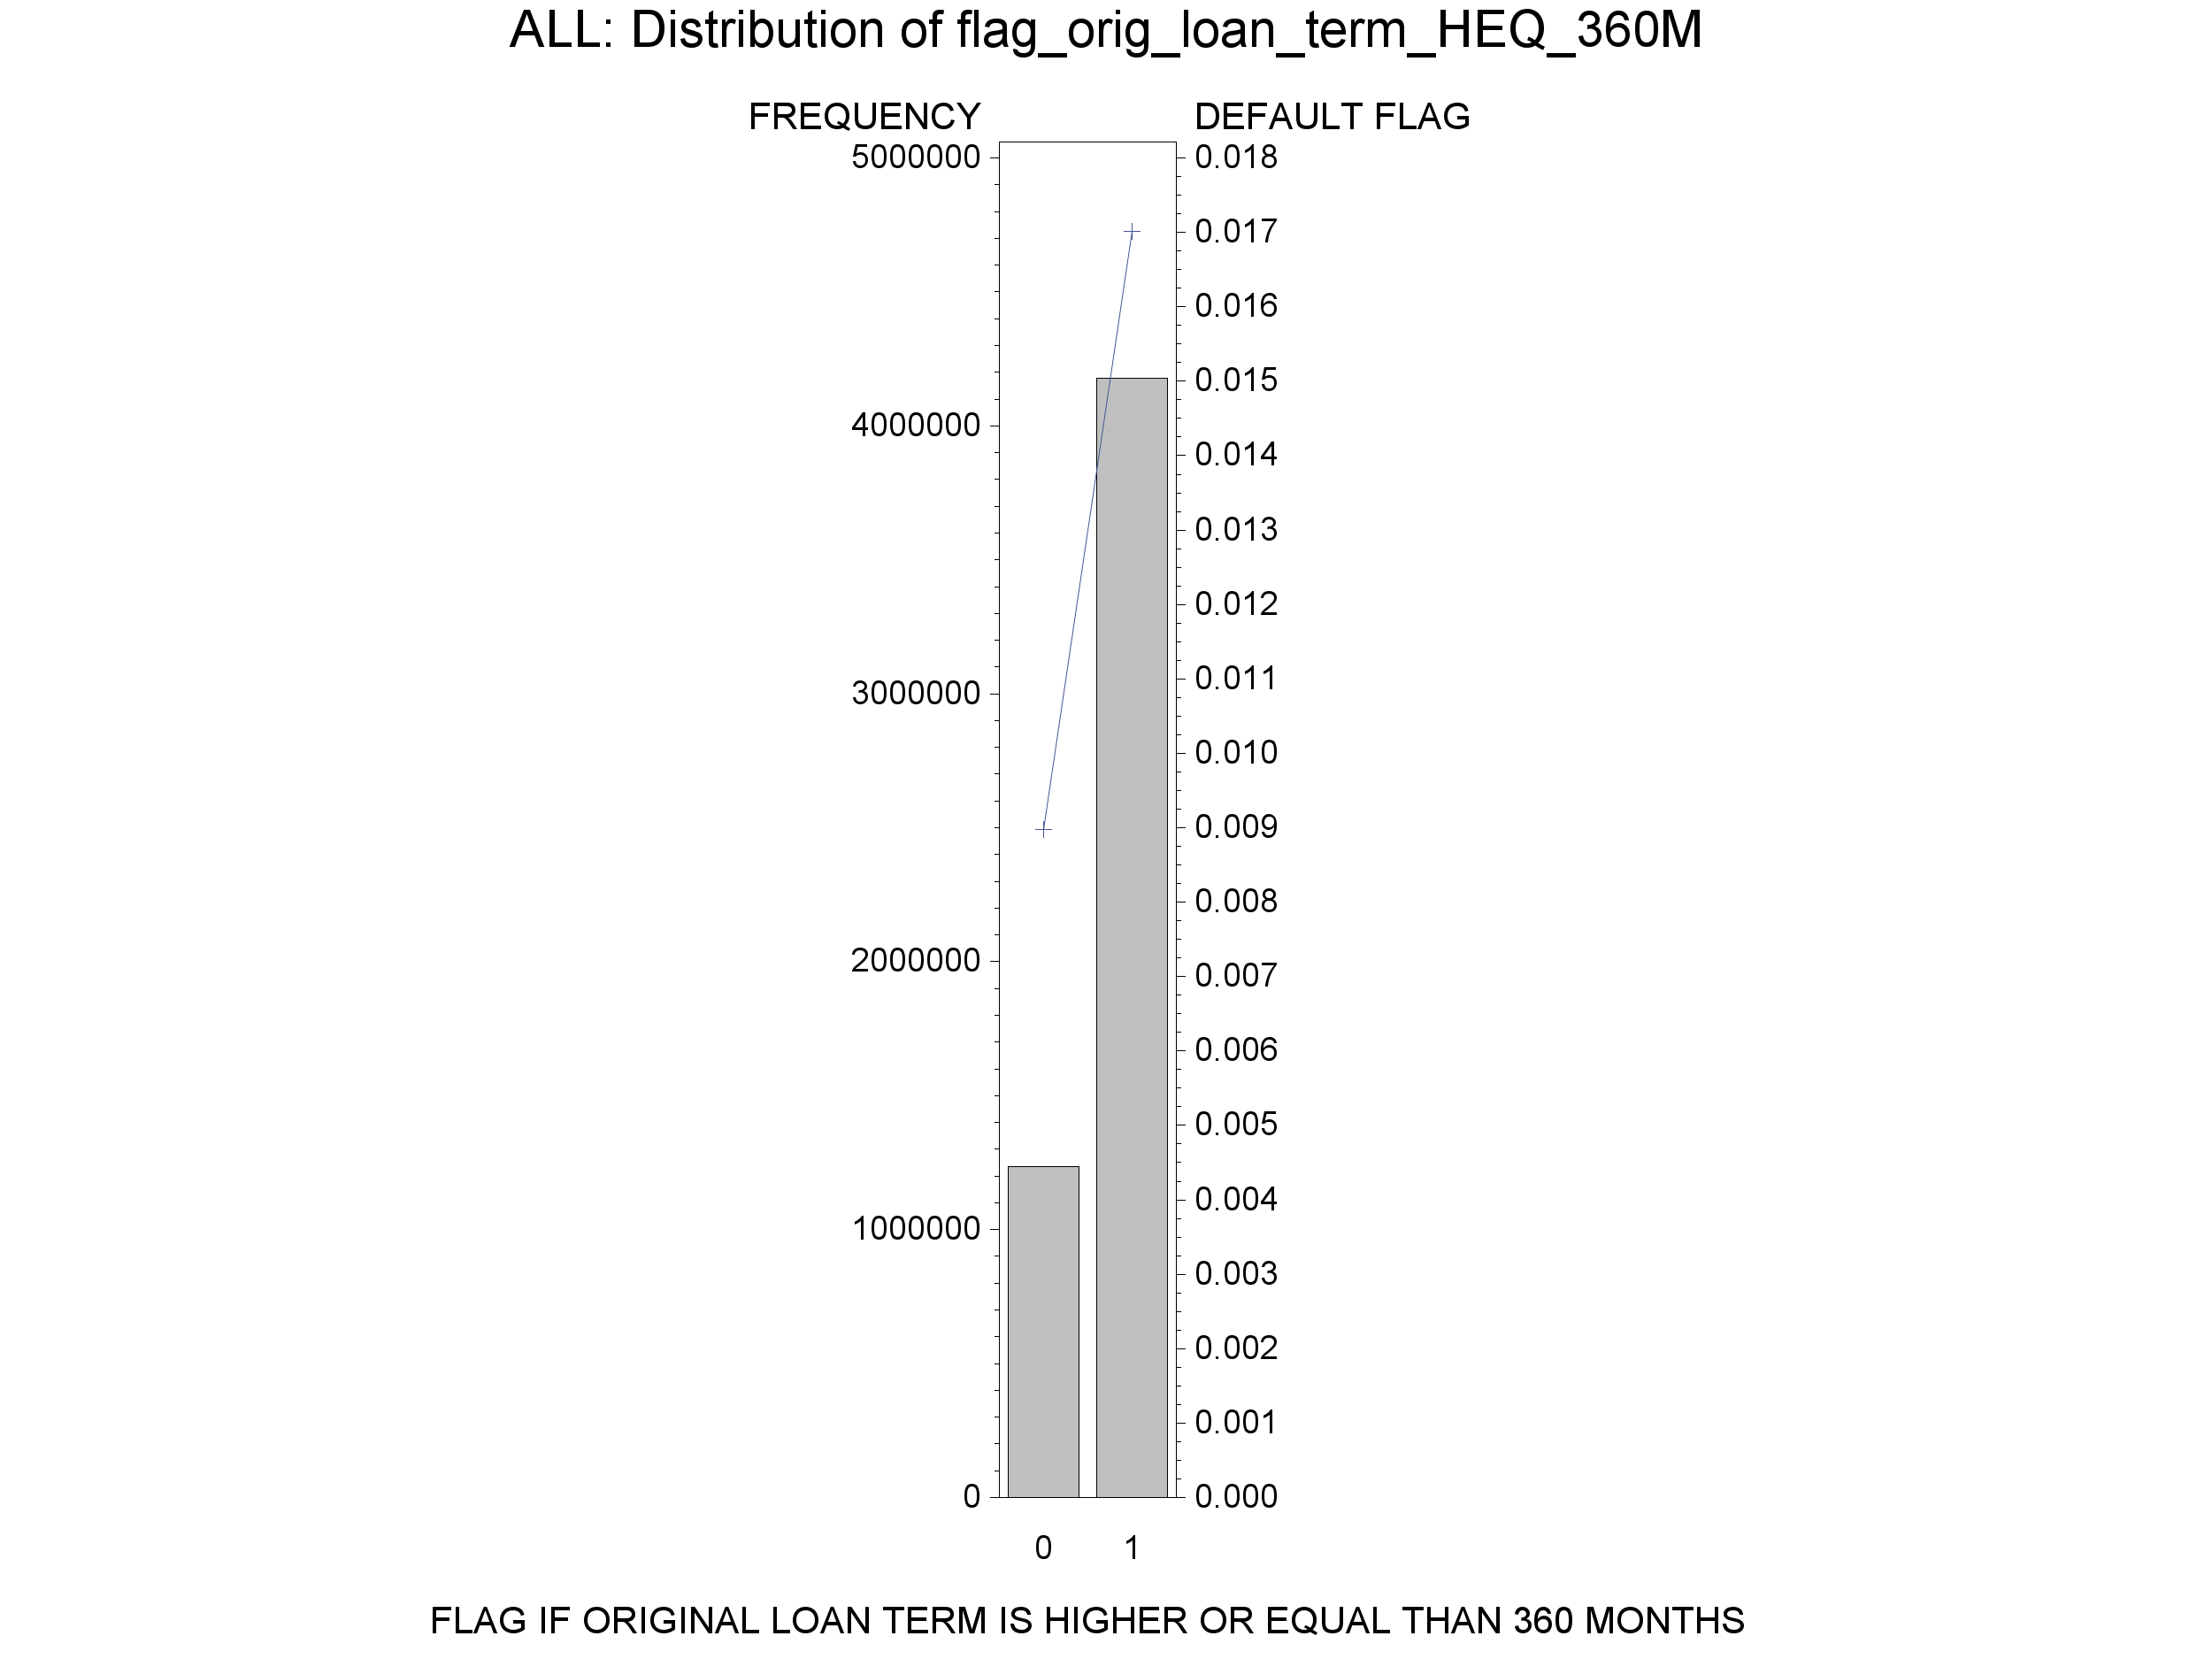
\includegraphics[width=0.9\textwidth]{./plot/Distribution/Main/RE_IND_flag_orig_loan_term_HEQ_360M_DISTRIBUTION_ALL.png}
\end{minipage}%
\begin{minipage}{.5\textwidth}
	\centering
	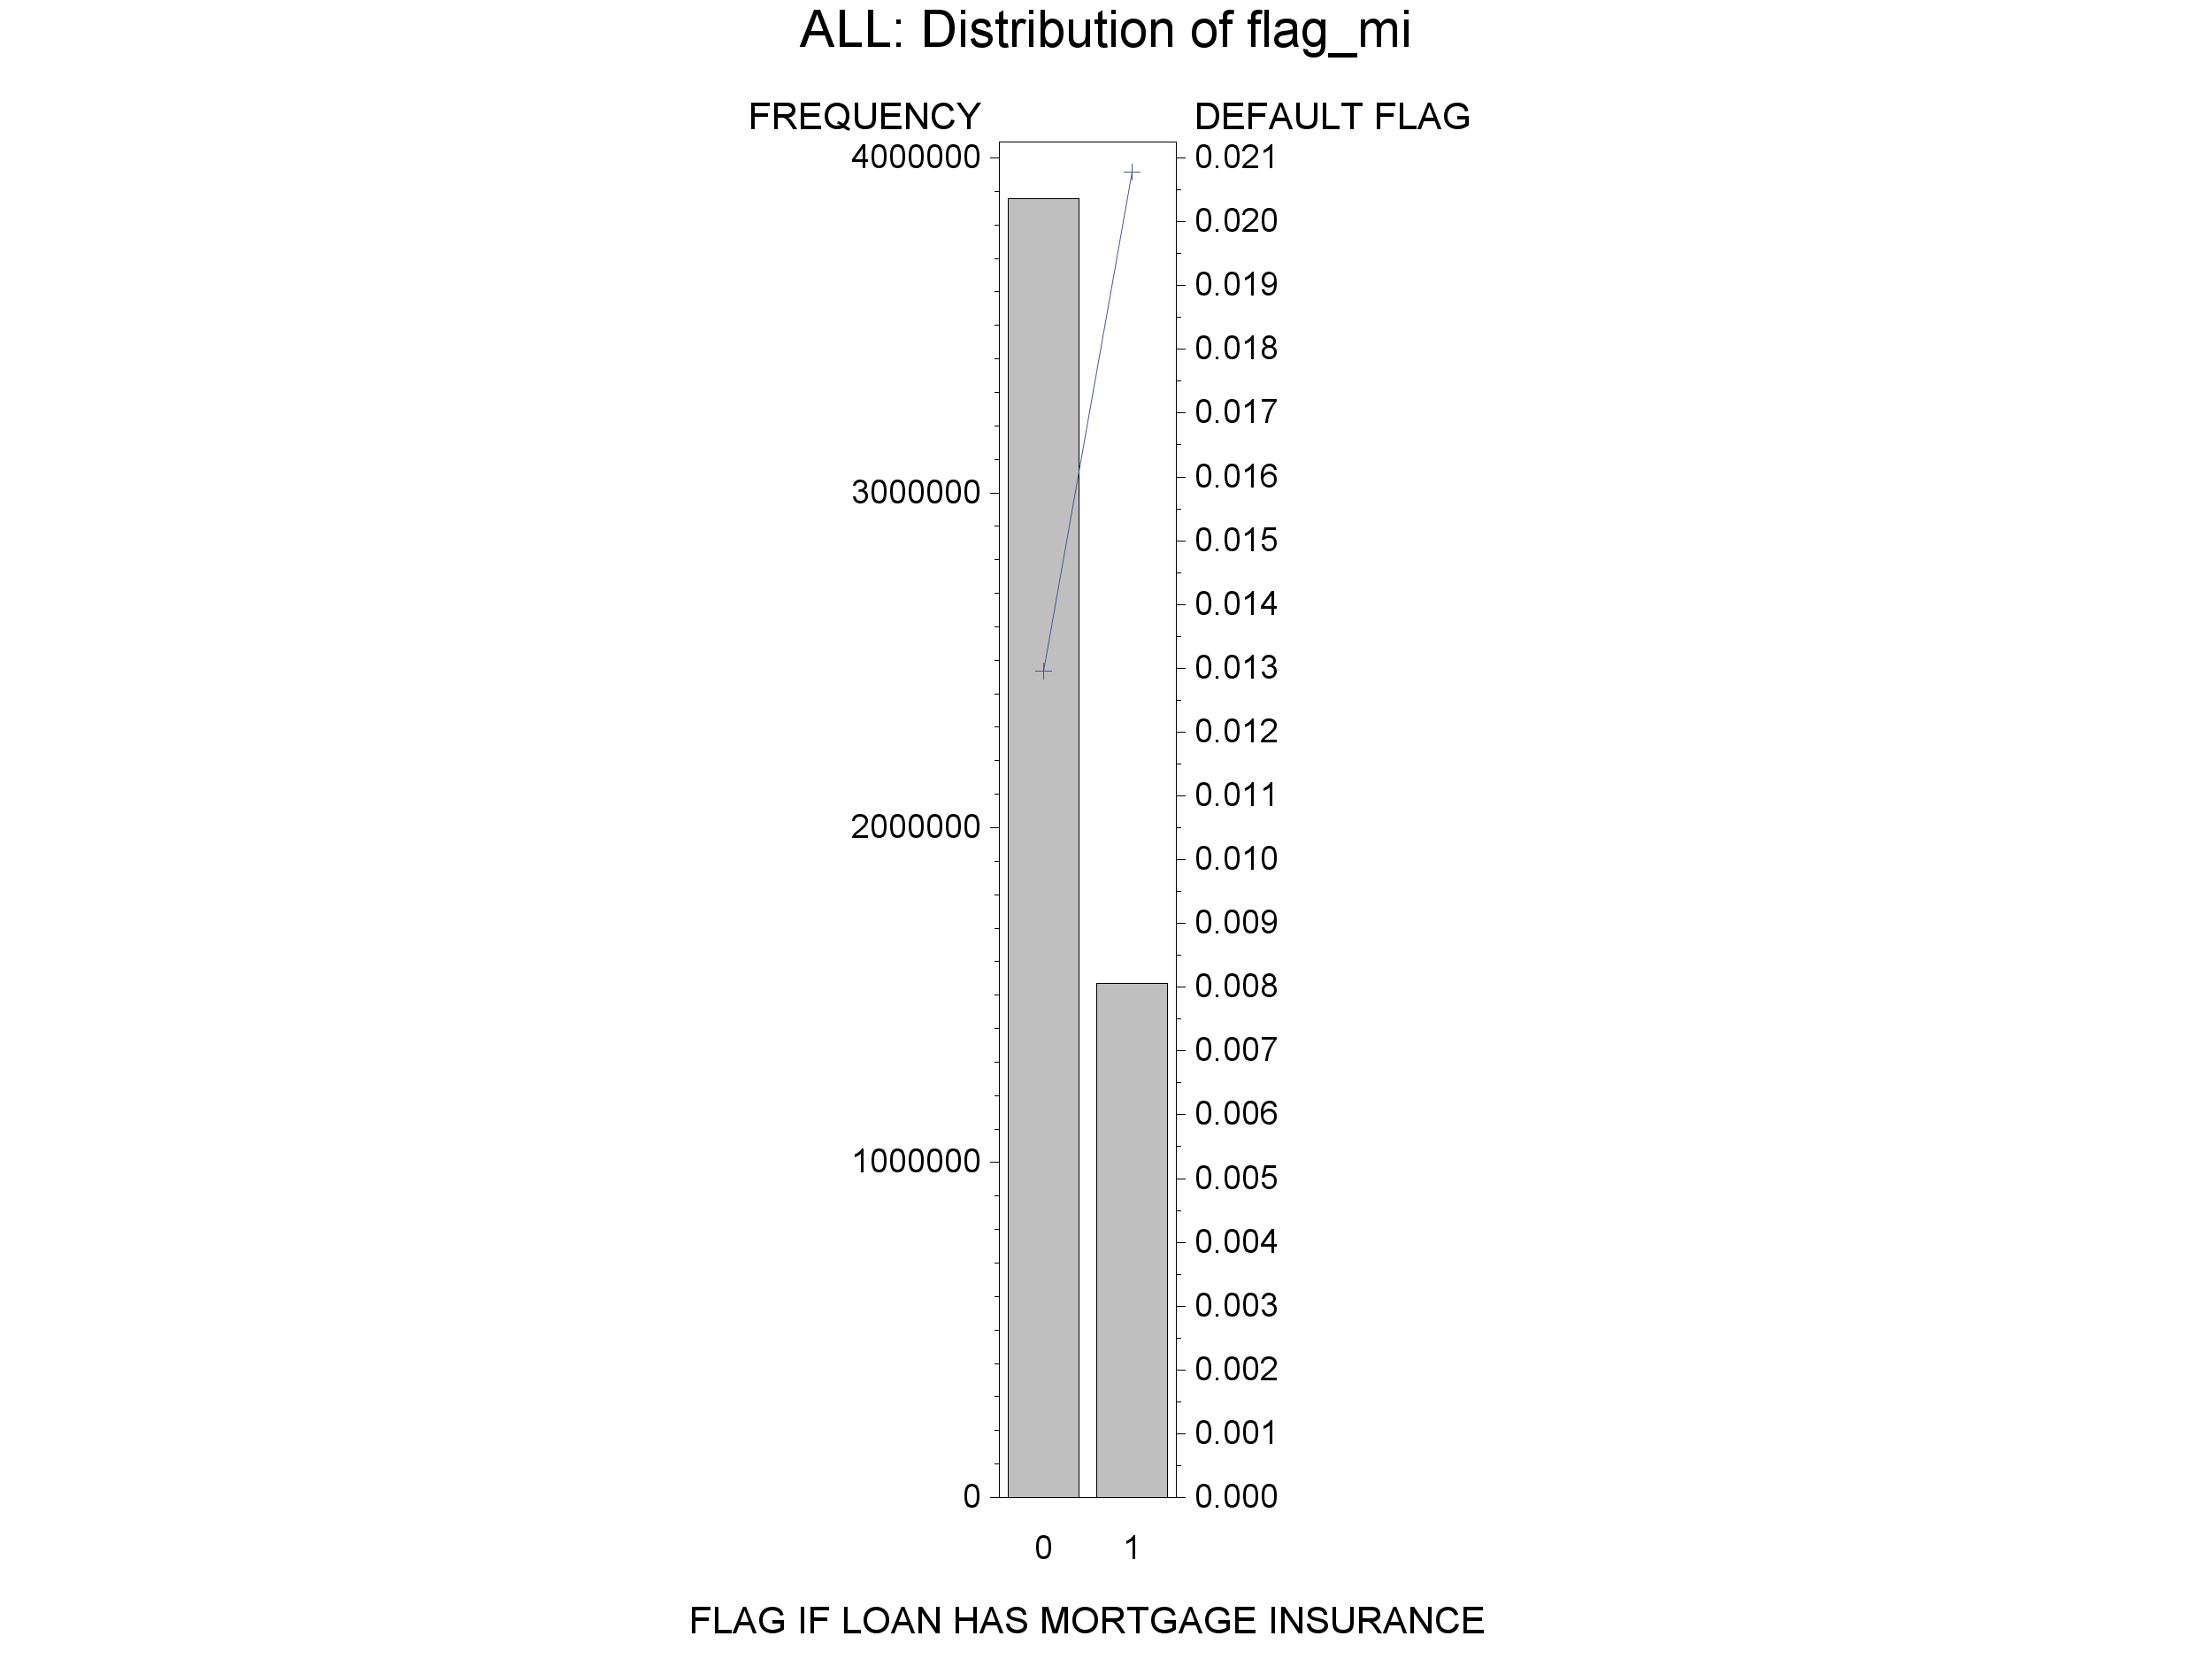
\includegraphics[width=0.9\textwidth]{./plot/Distribution/IND_flag_mi_DISTRIBUTION_ALL.png}
\end{minipage}
    \caption{Distribution and default rate of Loan Term $\geq$ 360m and MI Flag}
\end{figure}

\begin{figure}[H]
\begin{minipage}{.5\textwidth}
	\centering
	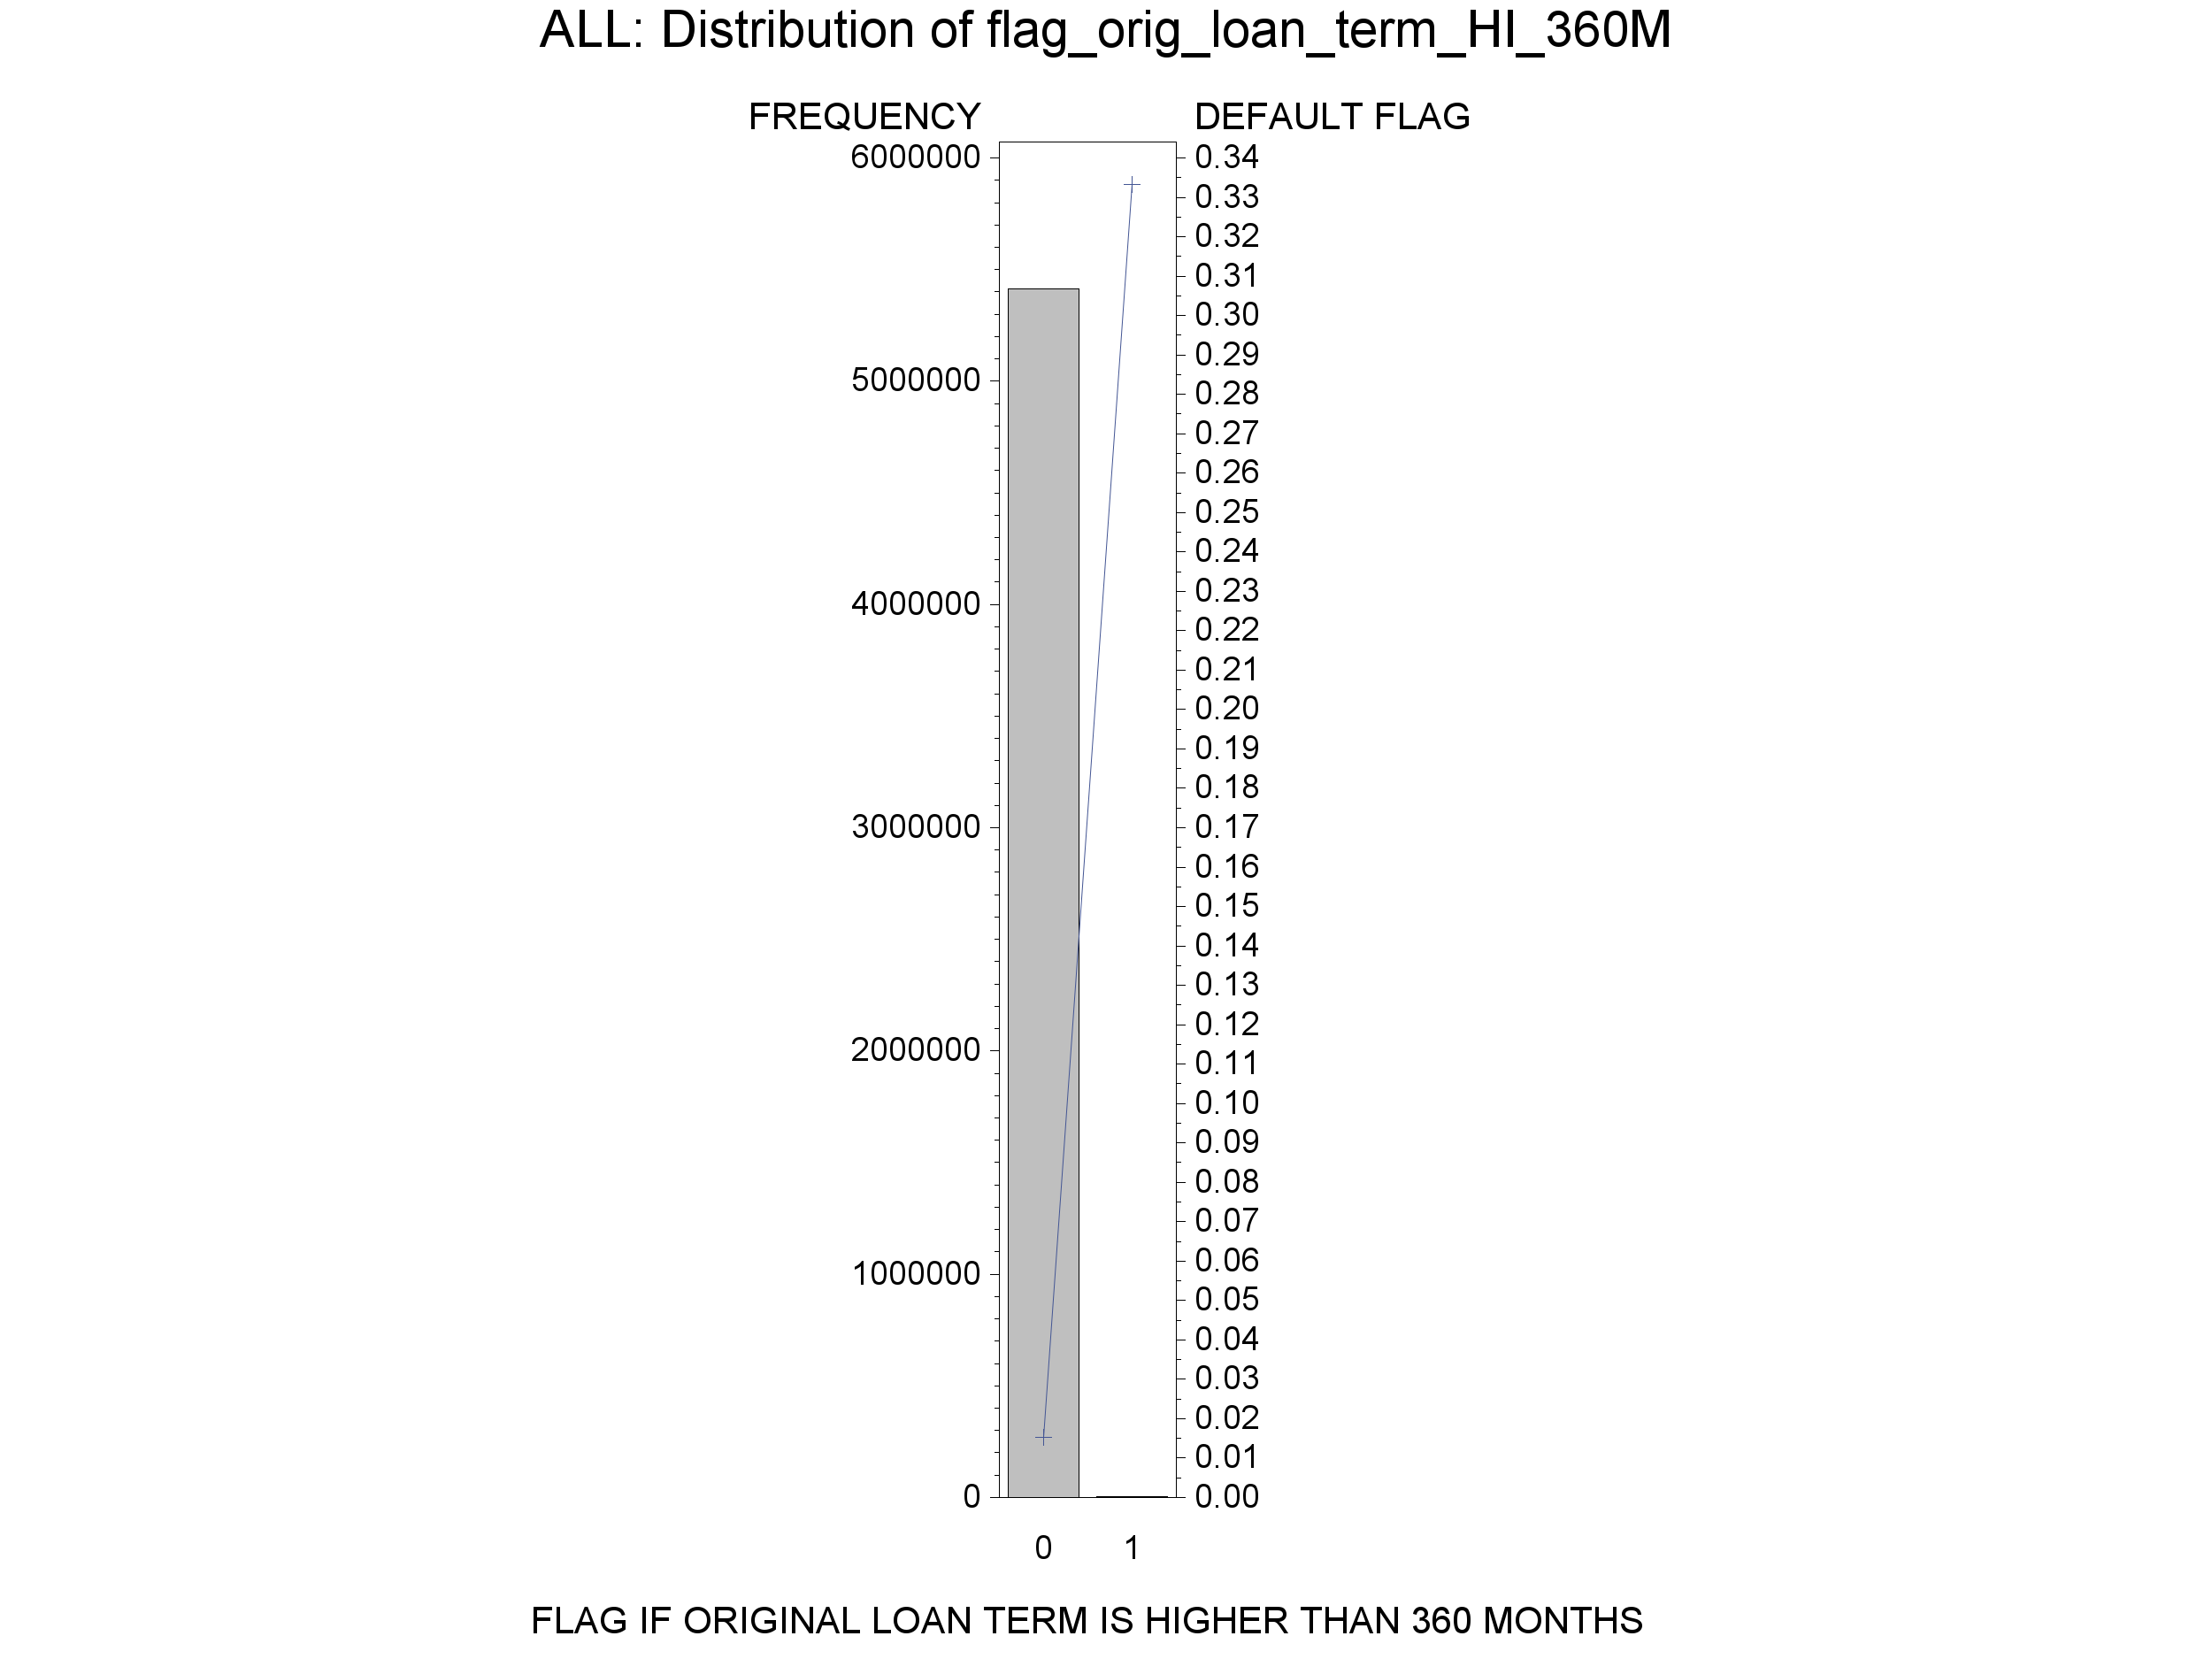
\includegraphics[width=0.9\textwidth]{./plot/Distribution/IND_flag_orig_loan_term_HI_360M_DISTRIBUTION_ALL.png}
\end{minipage}%
\begin{minipage}{.5\textwidth}
	\centering
	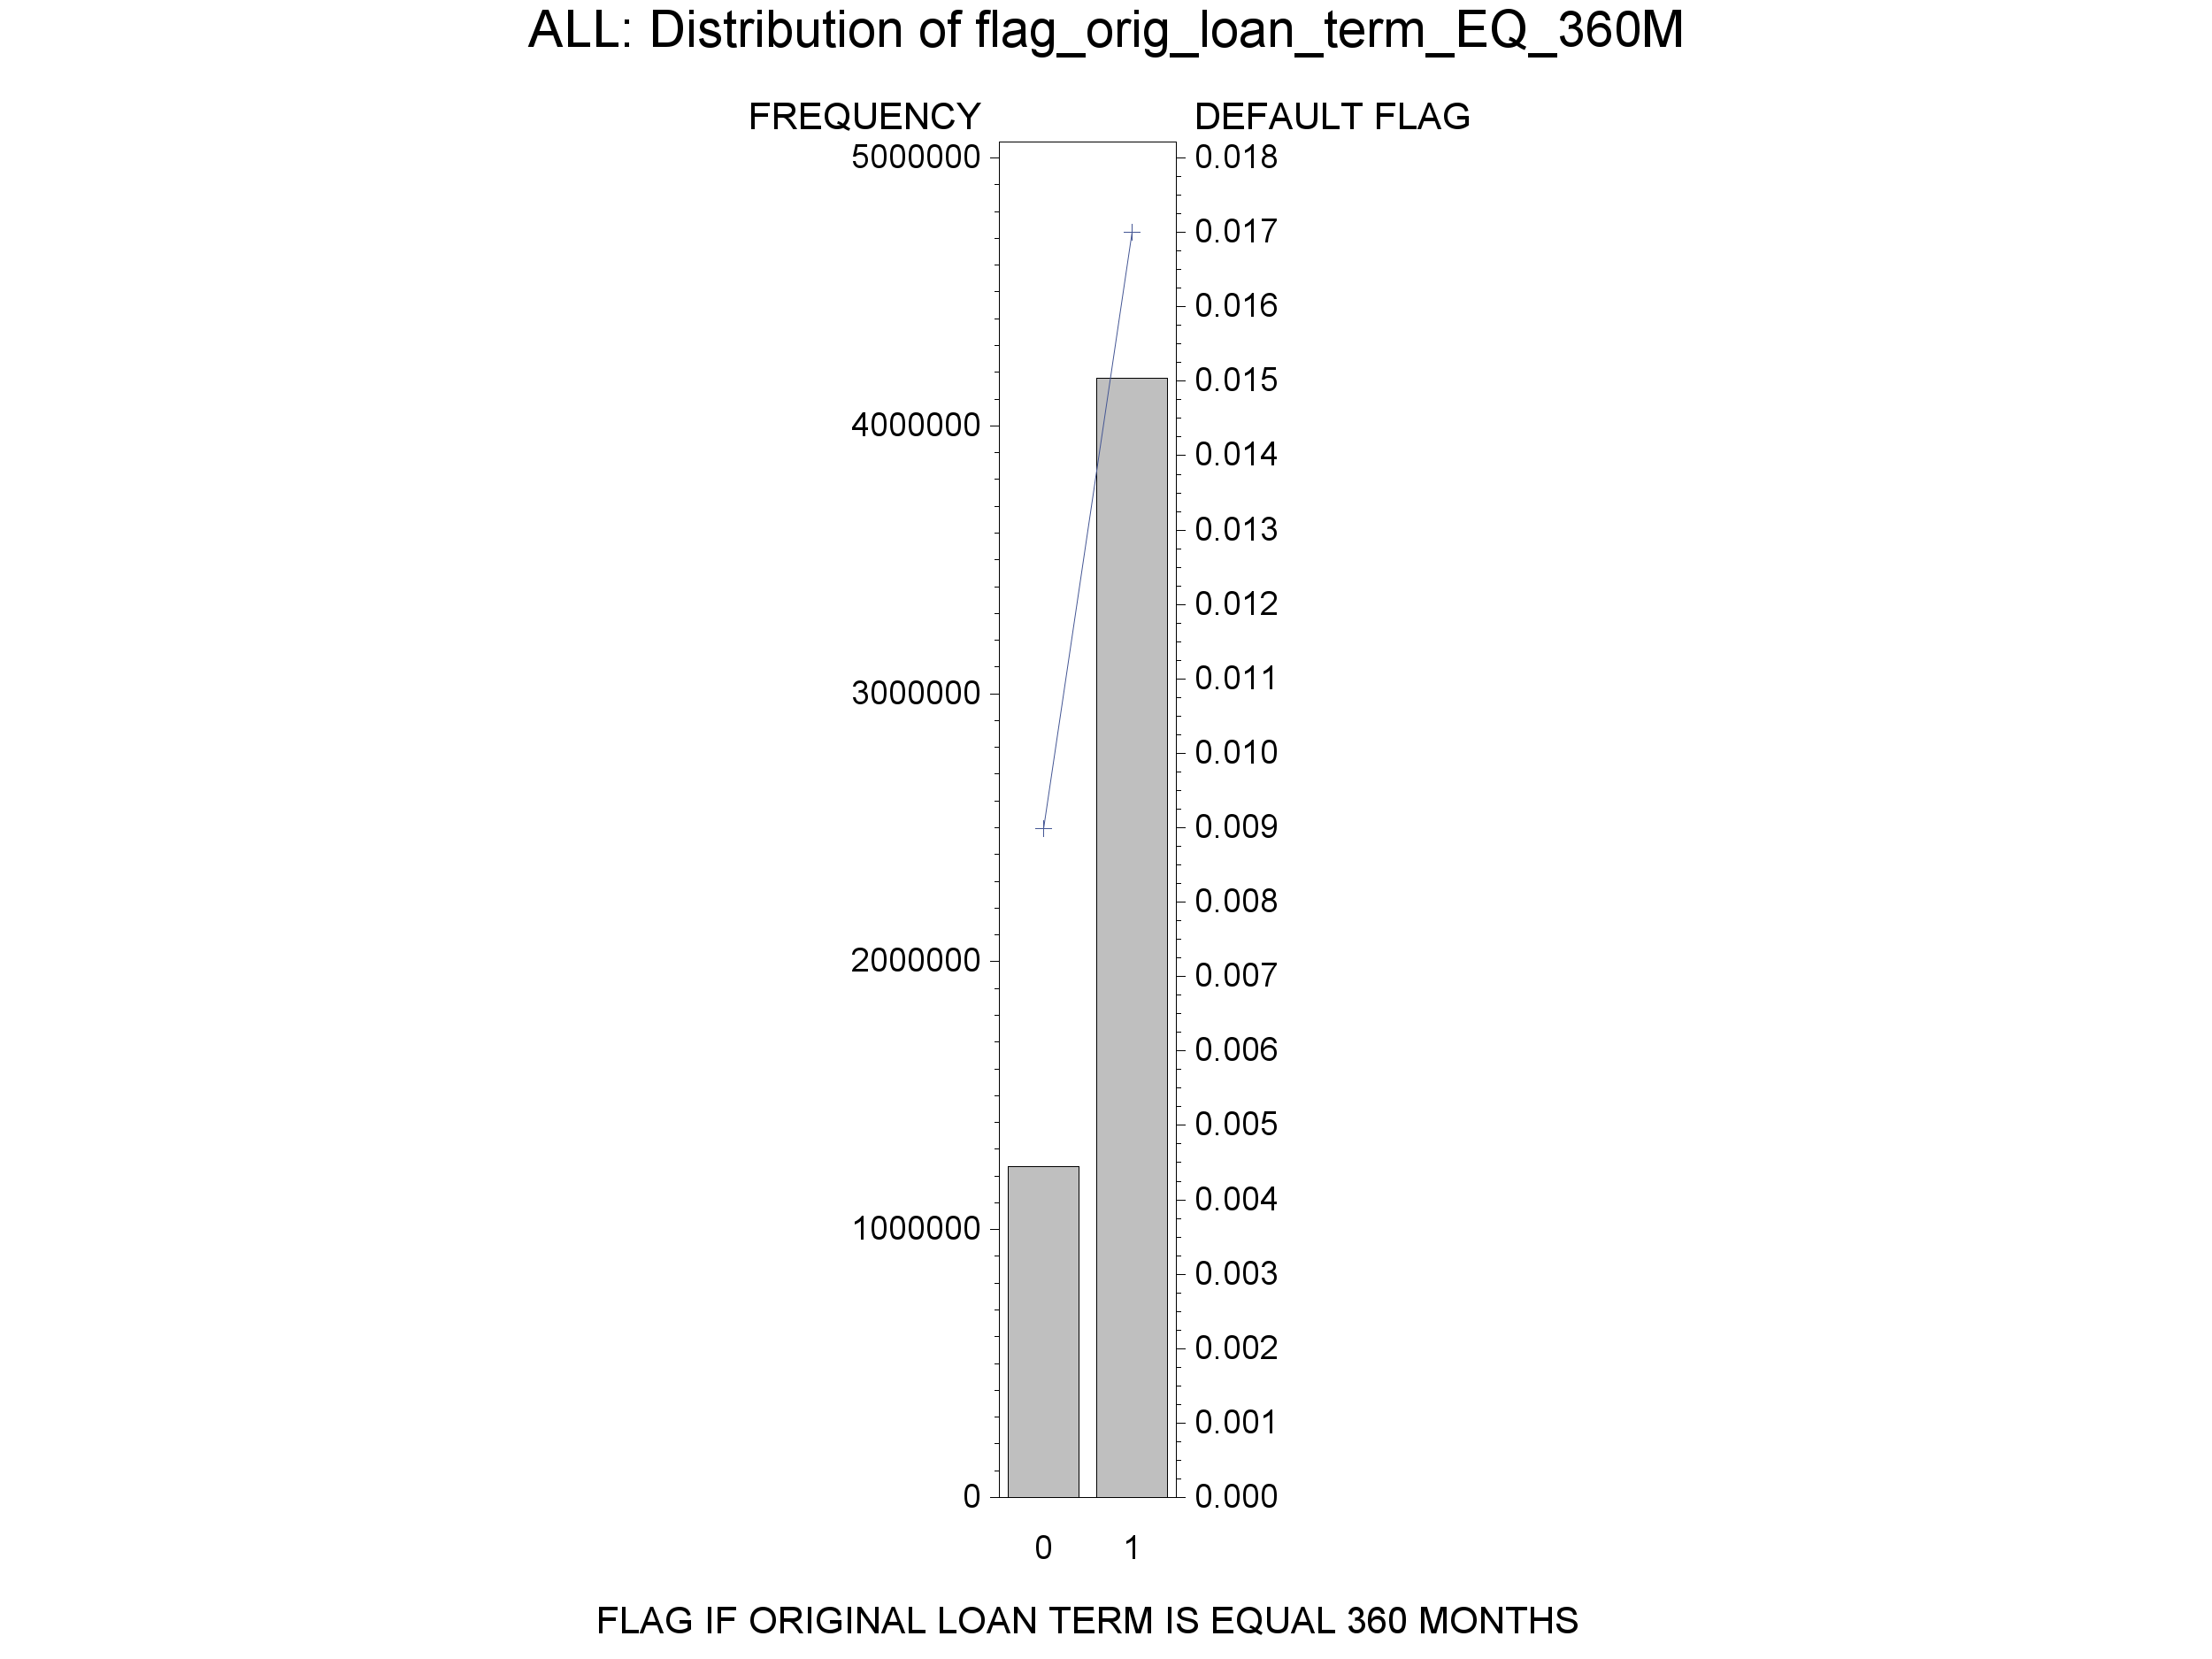
\includegraphics[width=0.9\textwidth]{./plot/Distribution/IND_flag_orig_loan_term_EQ_360M_DISTRIBUTION_ALL.png}
\end{minipage}
    \caption{Distribution and default rate of Loan Term > 360m and Loan Term = 360m}
\end{figure}

\begin{figure}[H]
\begin{minipage}{.5\textwidth}
	\centering
	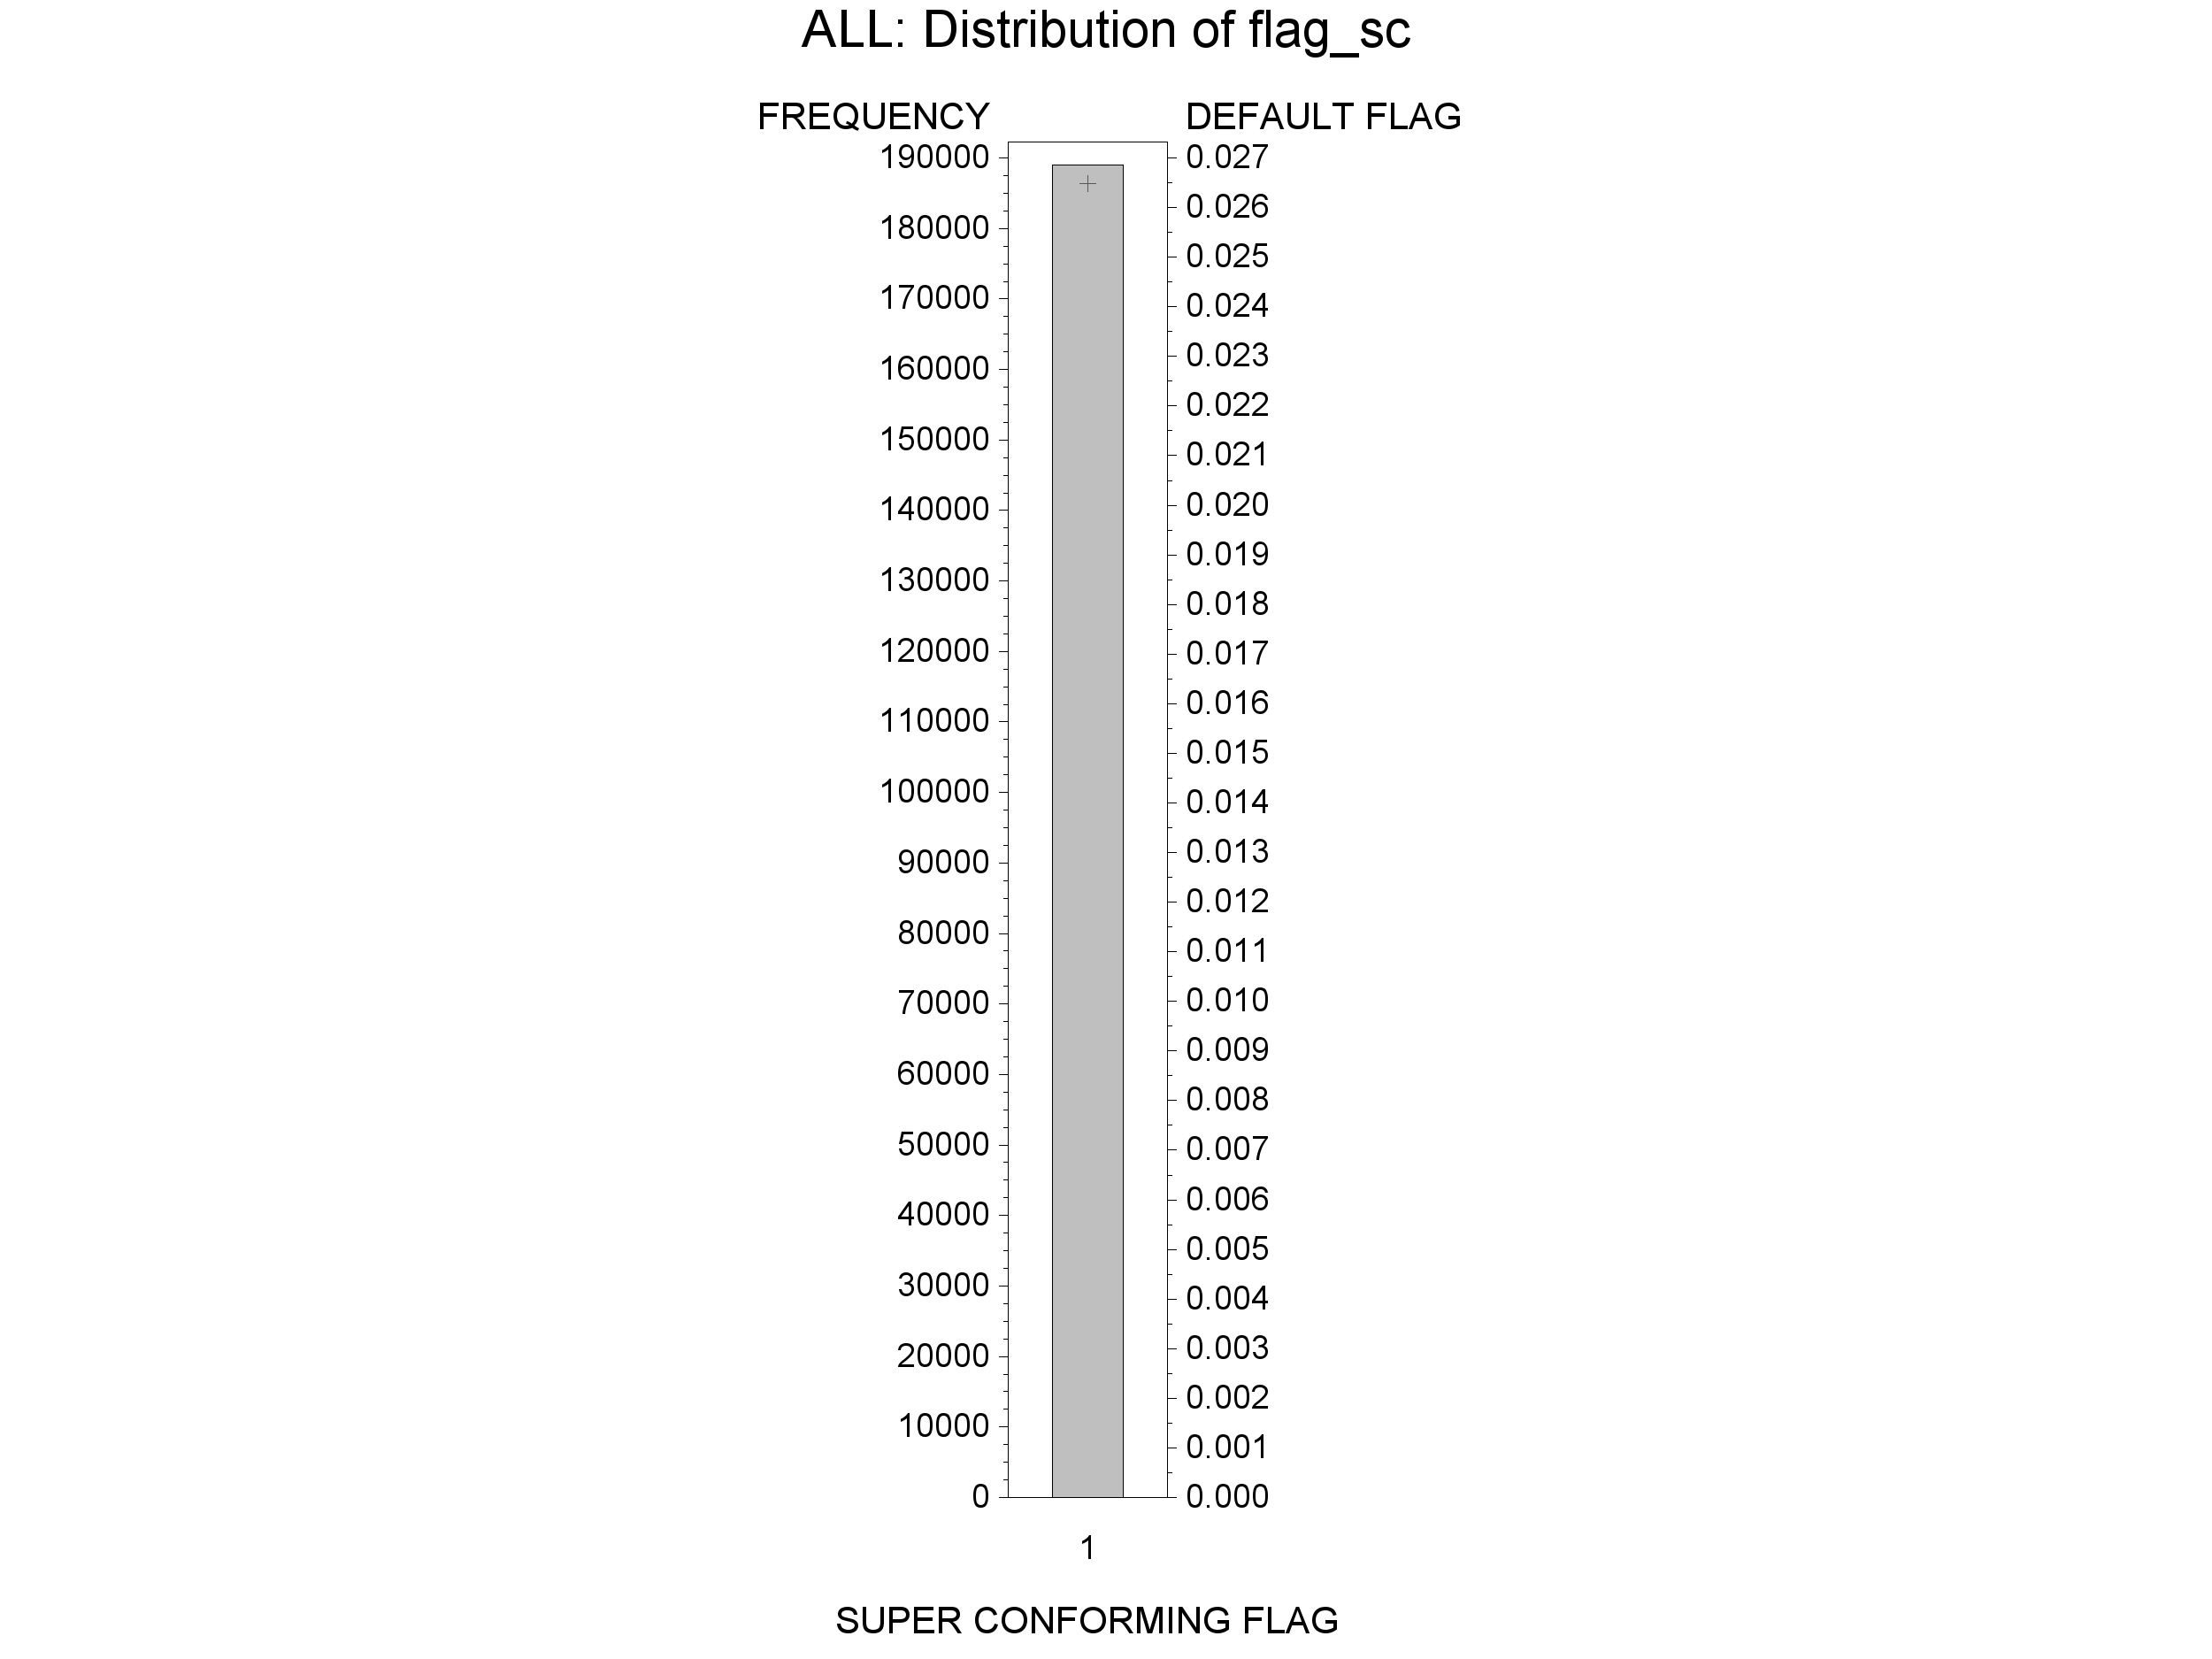
\includegraphics[width=0.9\textwidth]{./plot/Distribution/IND_flag_sc_DISTRIBUTION_ALL.png}
\end{minipage}%
\begin{minipage}{.5\textwidth}
	\centering
	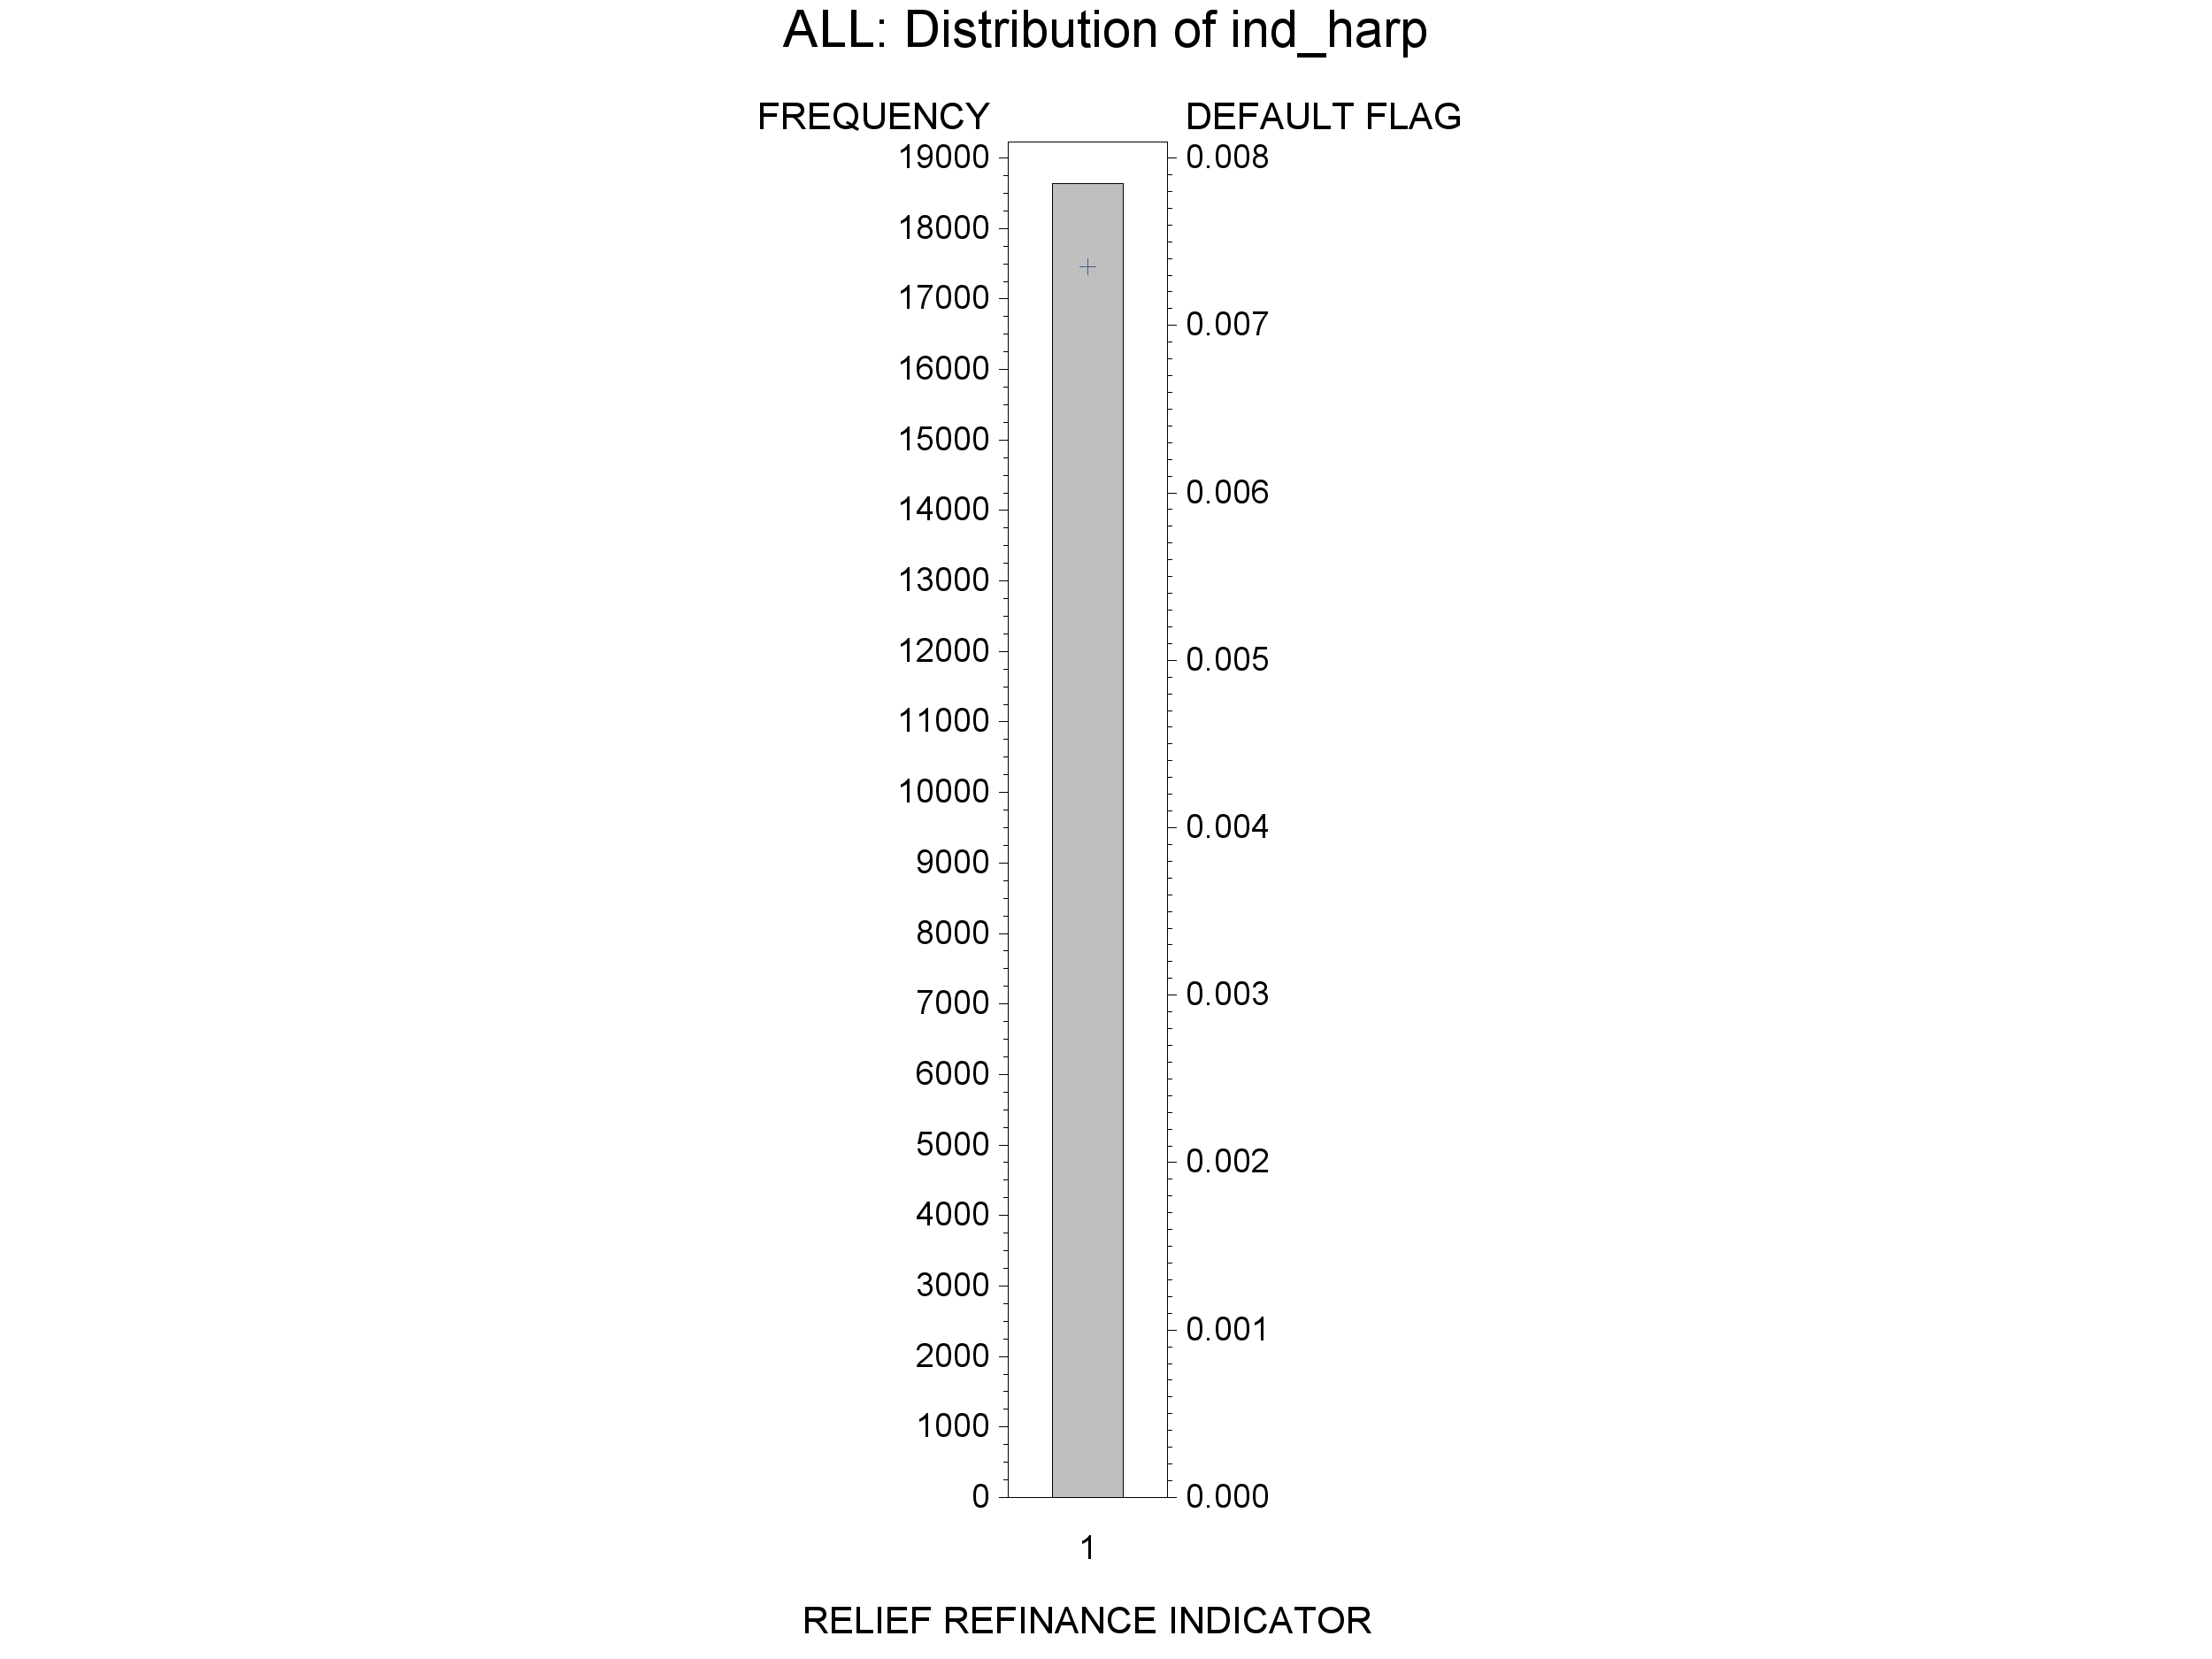
\includegraphics[width=0.9\textwidth]{./plot/Distribution/IND_ind_harp_DISTRIBUTION_ALL.png}
\end{minipage}
    \caption{Distribution and default rate of Sup Conf Flag and HARP Flag}
\end{figure}

\begin{figure}[H]
\begin{minipage}{.5\textwidth}
	\centering
	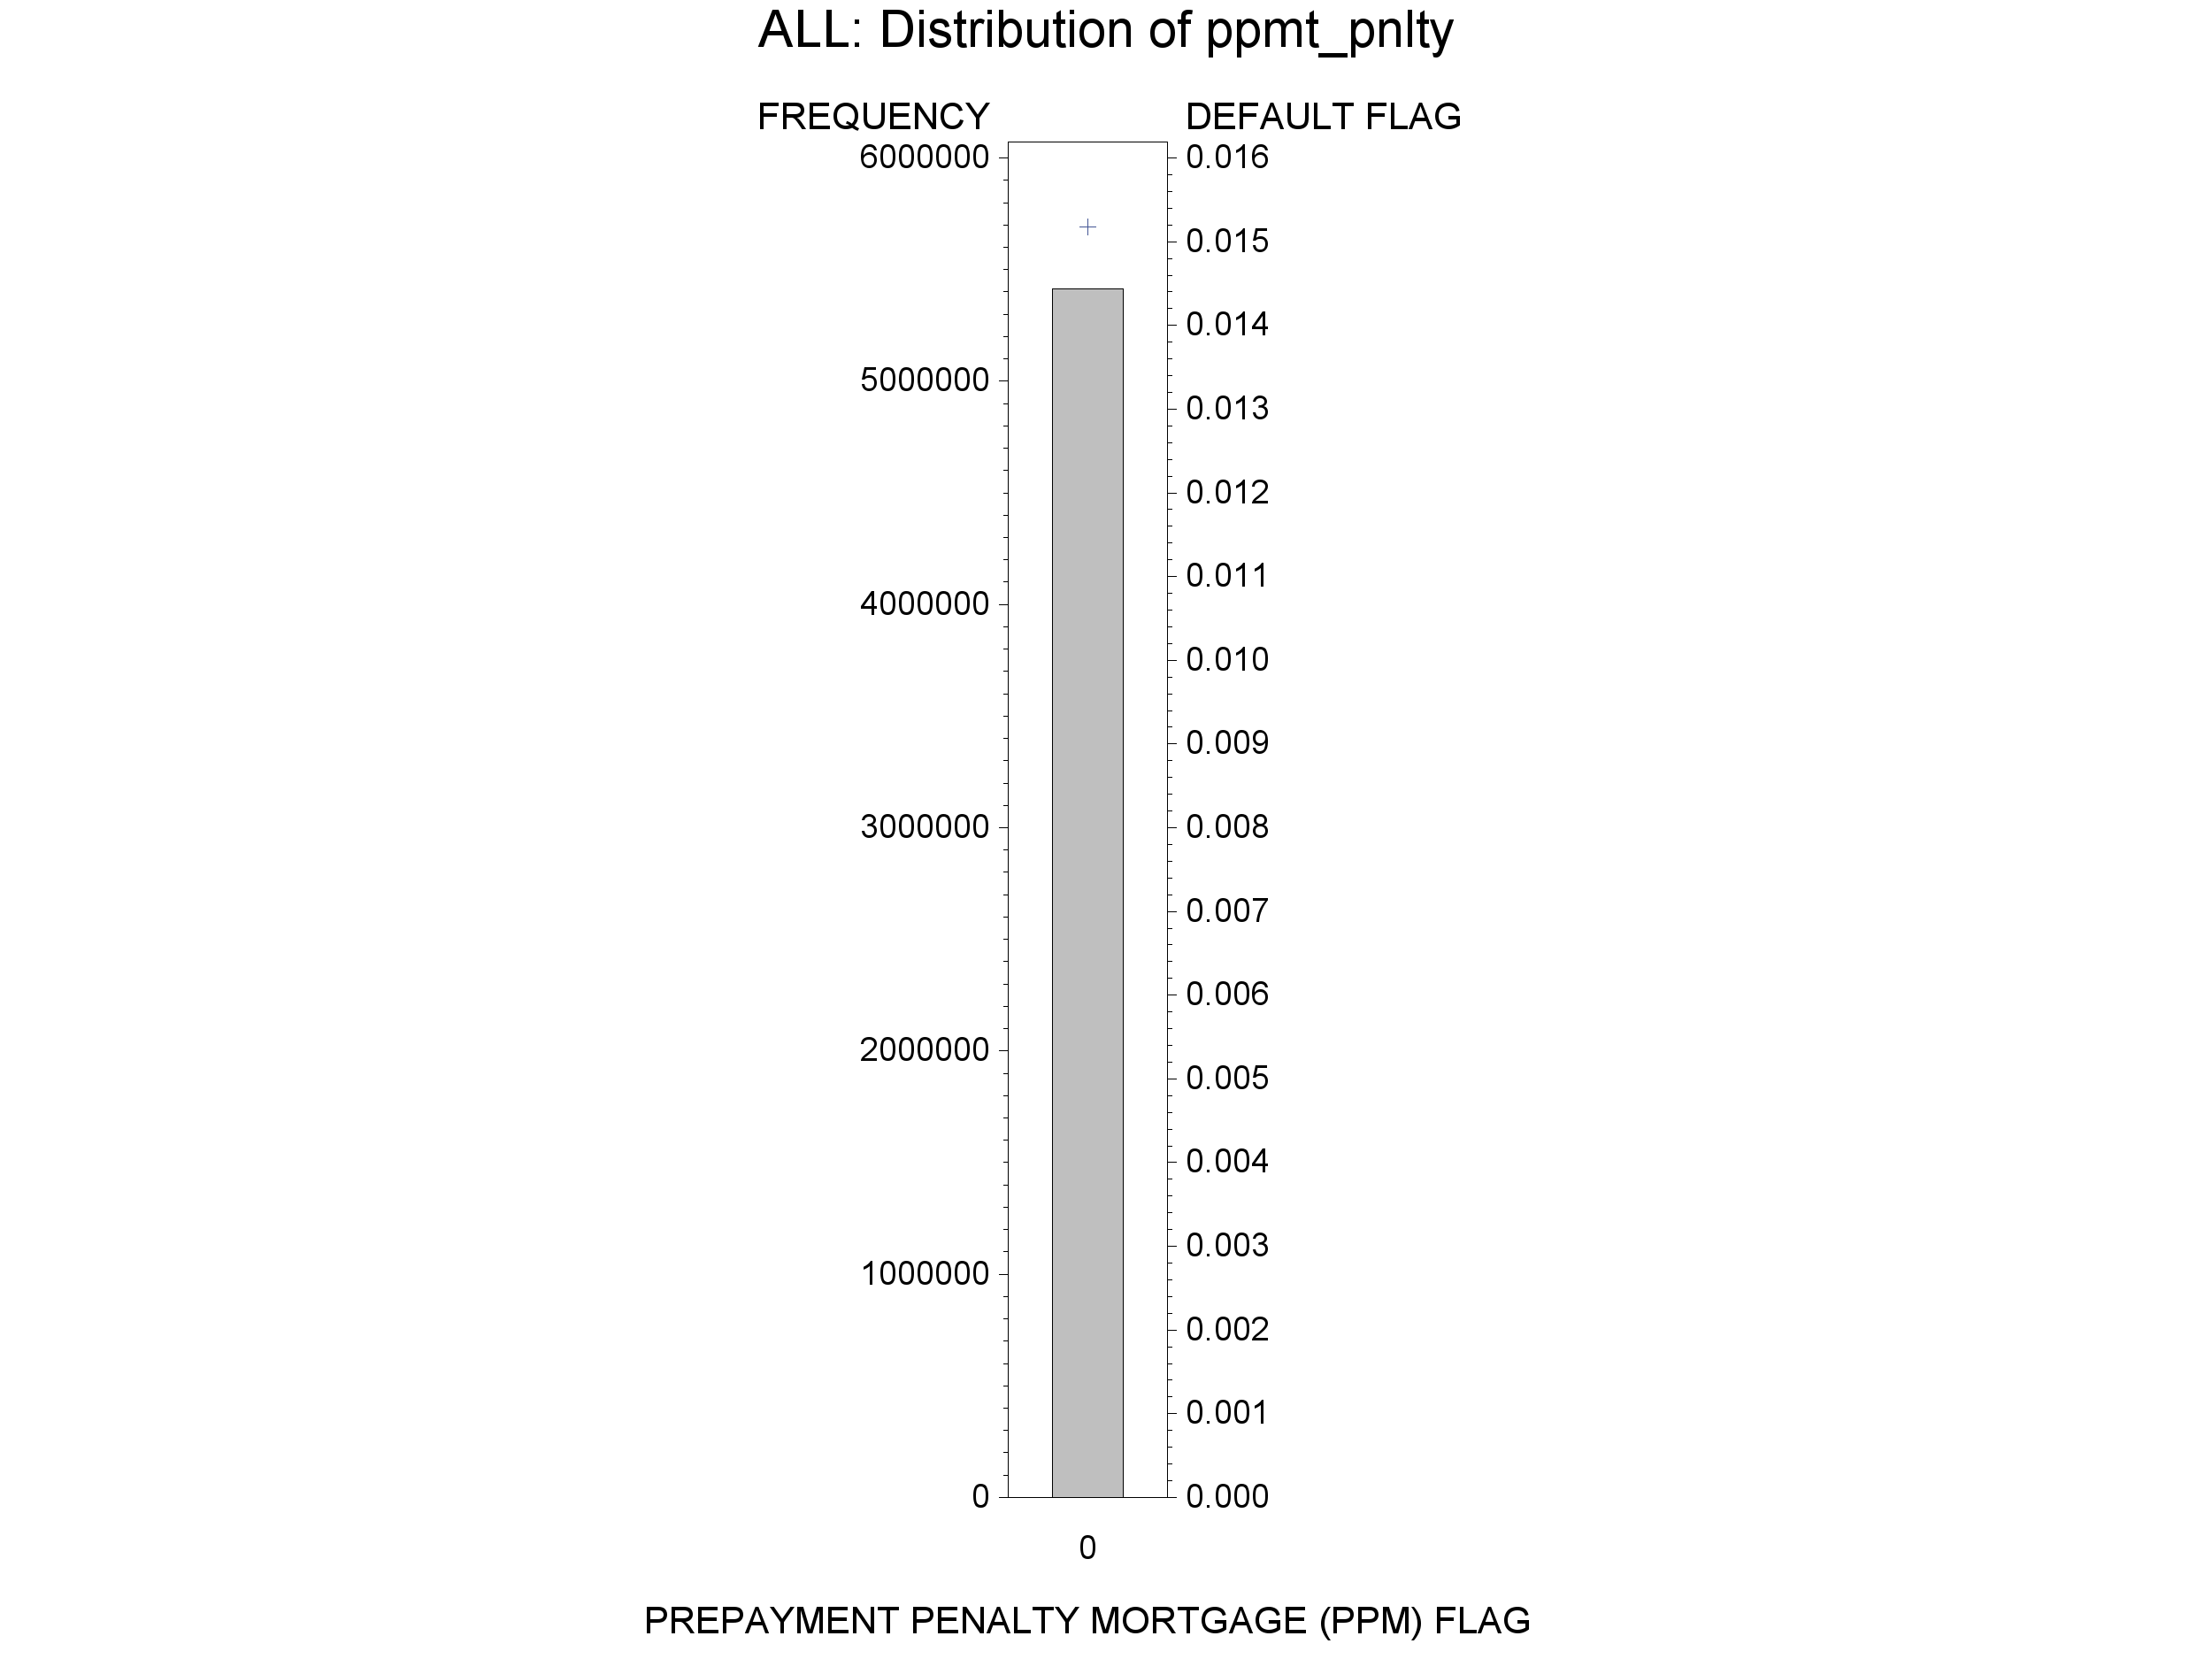
\includegraphics[width=0.9\textwidth]{./plot/Distribution/IND_ppmt_pnlty_DISTRIBUTION_ALL.png}
\end{minipage}%
\begin{minipage}{.5\textwidth}
	\centering
	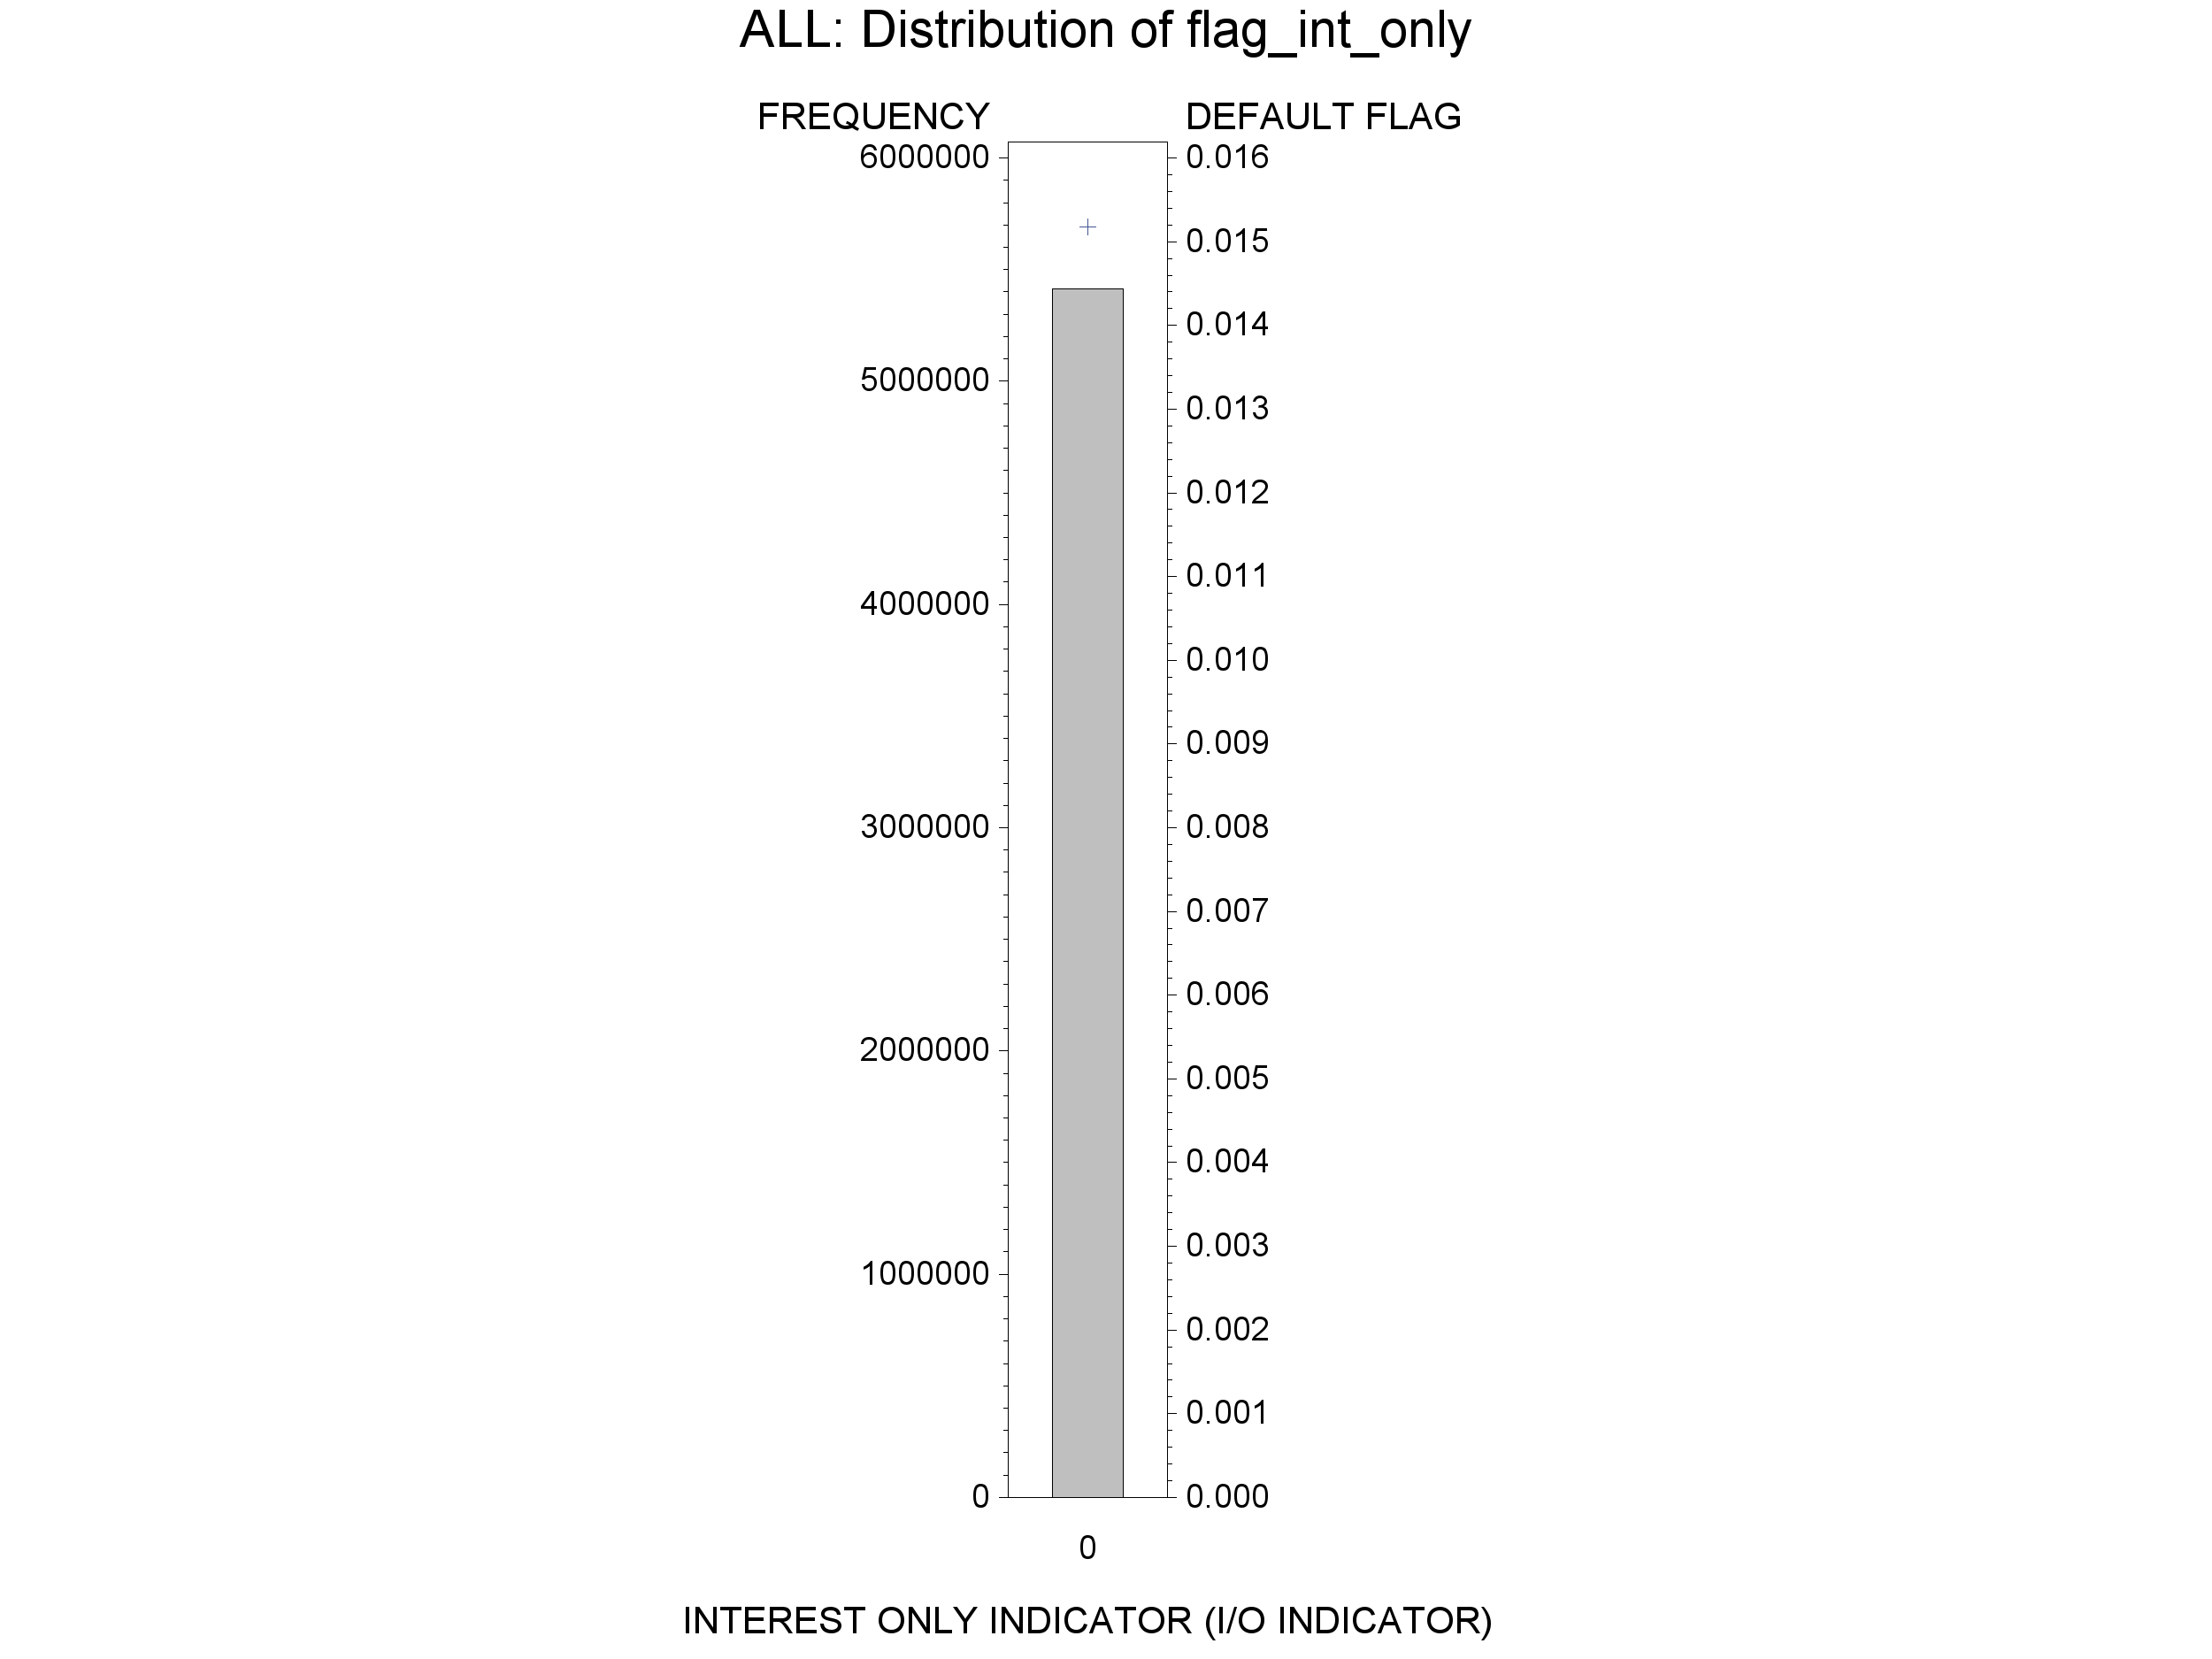
\includegraphics[width=0.9\textwidth]{./plot/Distribution/IND_flag_int_only_DISTRIBUTION_ALL.png}
\end{minipage}
    \caption{Distribution and default rate of PPM Flag and Int Only Flag}
\end{figure}

\begin{figure}[H]
\begin{minipage}{.5\textwidth}
	\centering
	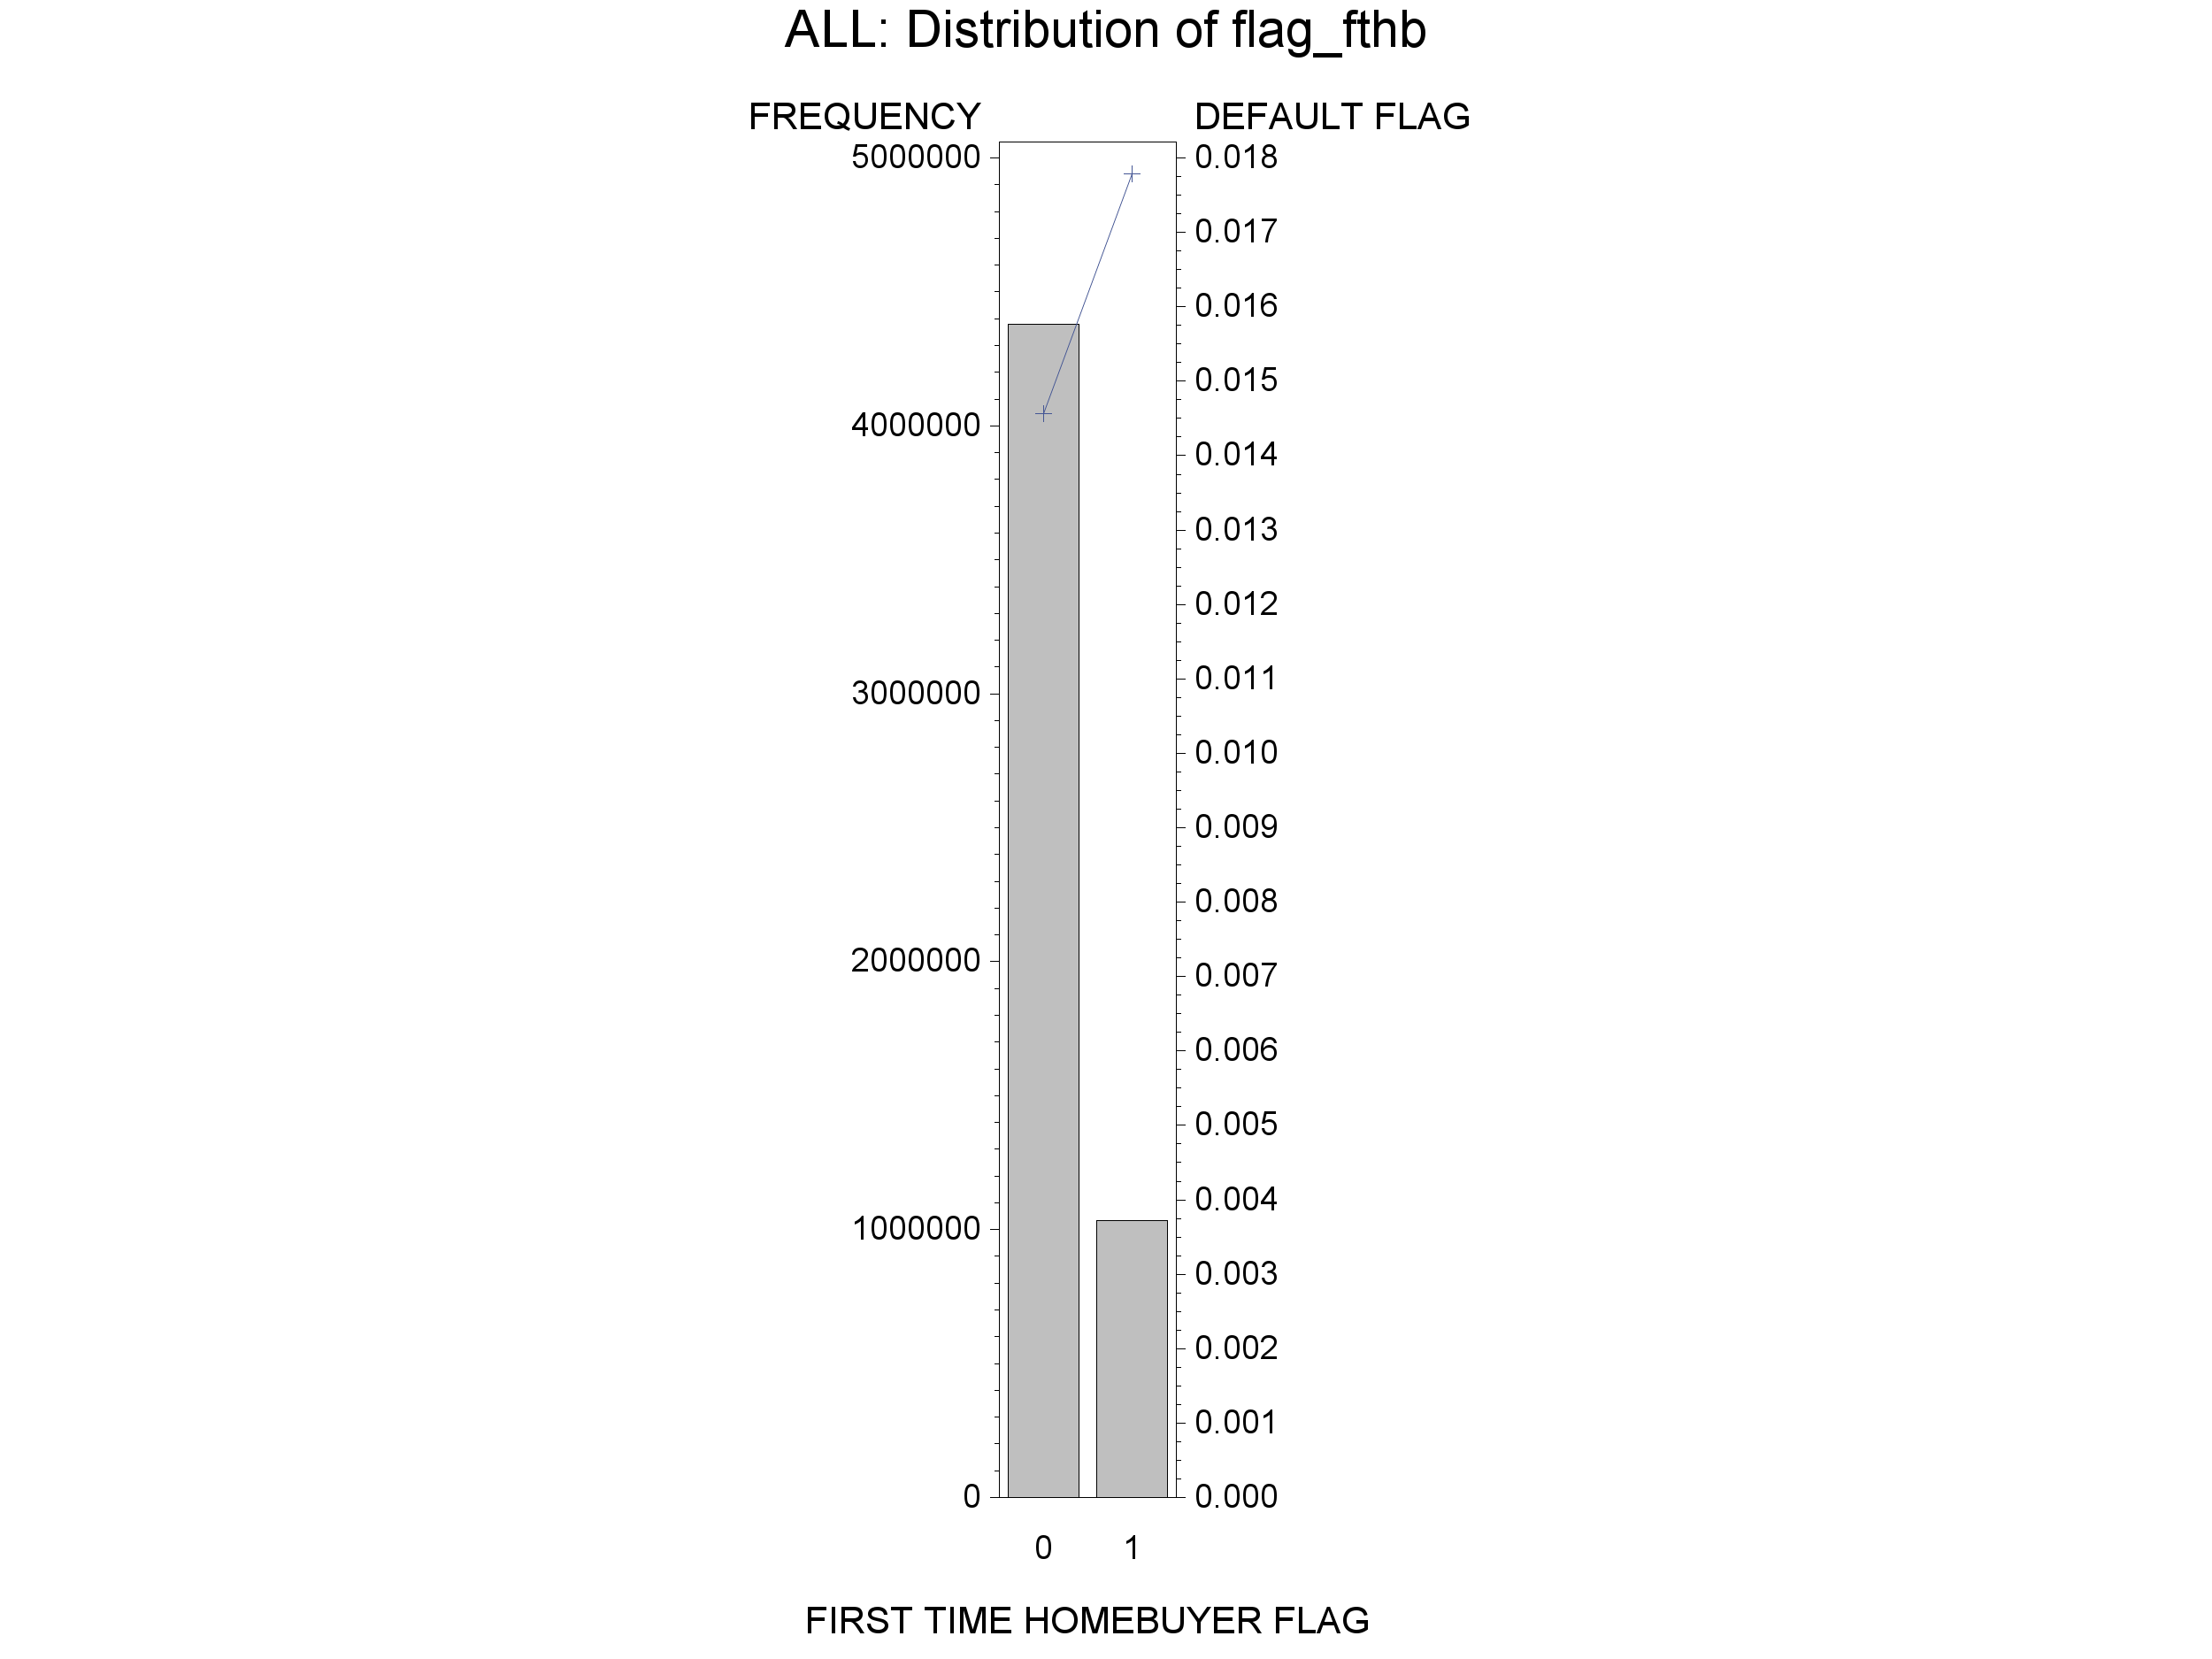
\includegraphics[width=0.9\textwidth]{./plot/Distribution/IND_flag_fthb_DISTRIBUTION_ALL.png}
\end{minipage}%
\begin{minipage}{.5\textwidth}
	\centering
	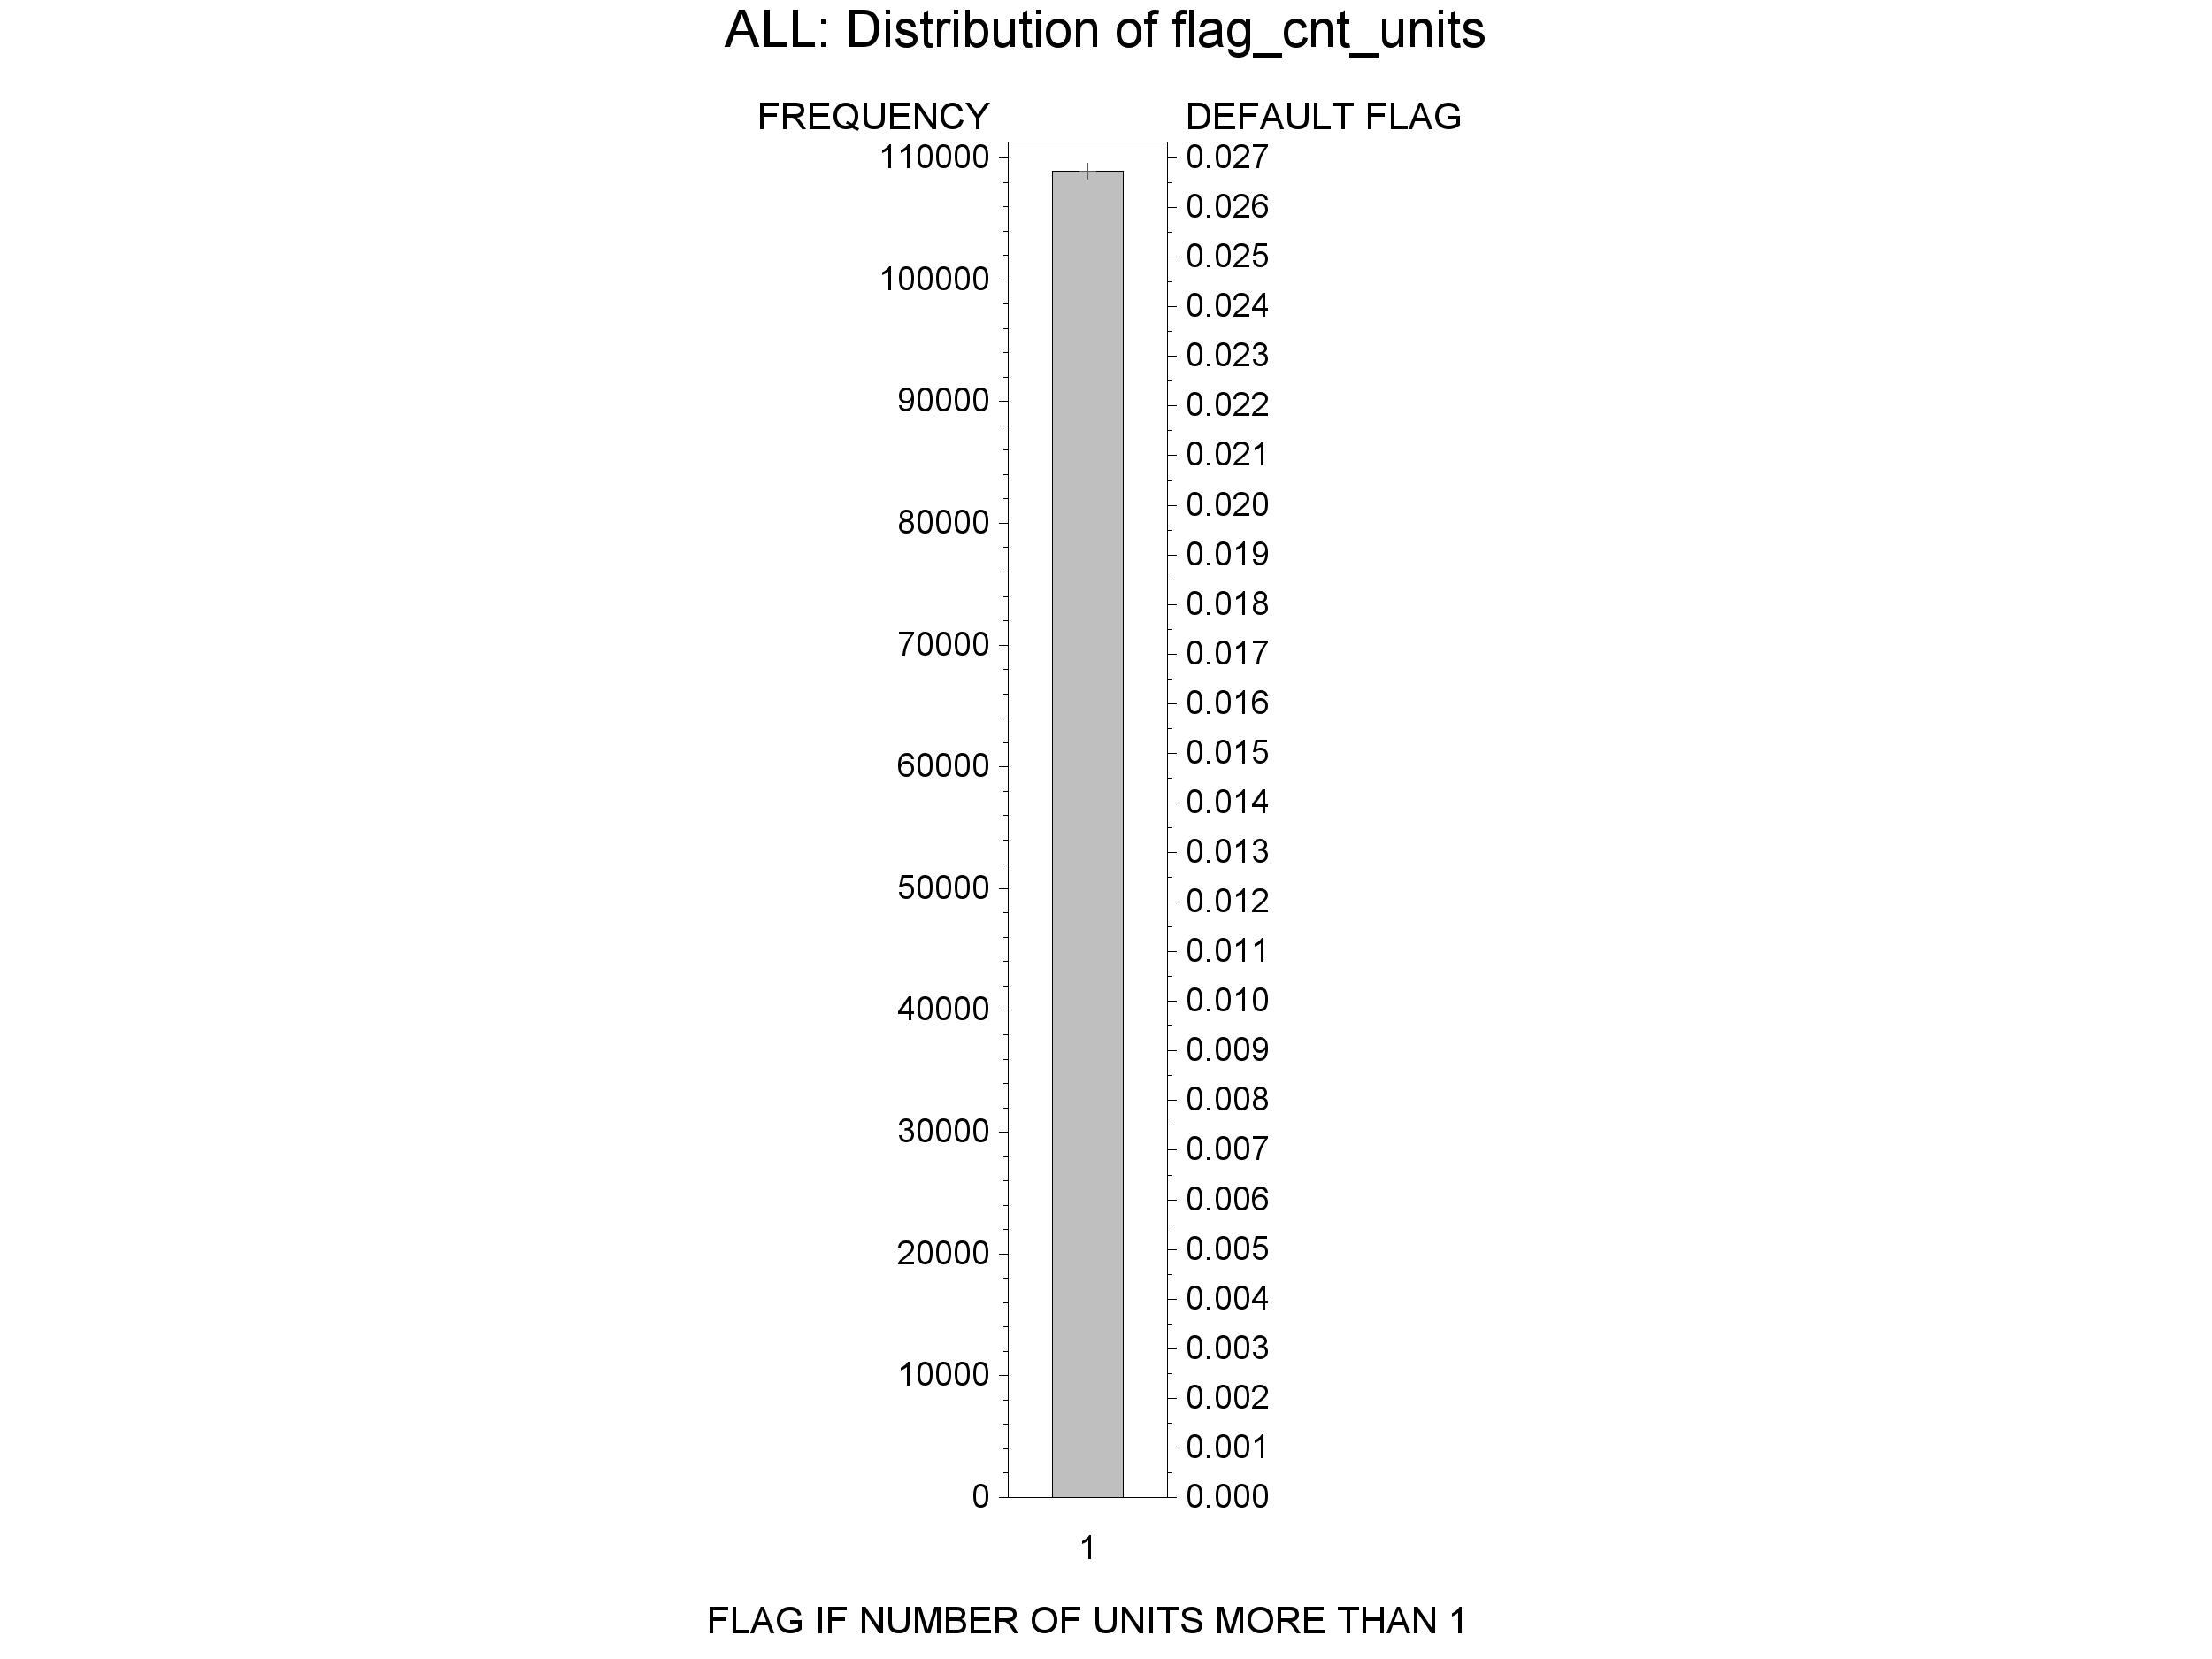
\includegraphics[width=0.9\textwidth]{./plot/Distribution/IND_flag_cnt_units_DISTRIBUTION_ALL.png}
\end{minipage}
    \caption{Distribution and default rate of US region and Loan Term (grouped)}
\end{figure}


\section{Boxplots of all numerical variables}
\label{sec:boxplot_all}

\begin{figure}[H]
\begin{minipage}{.5\textwidth}
	\centering
	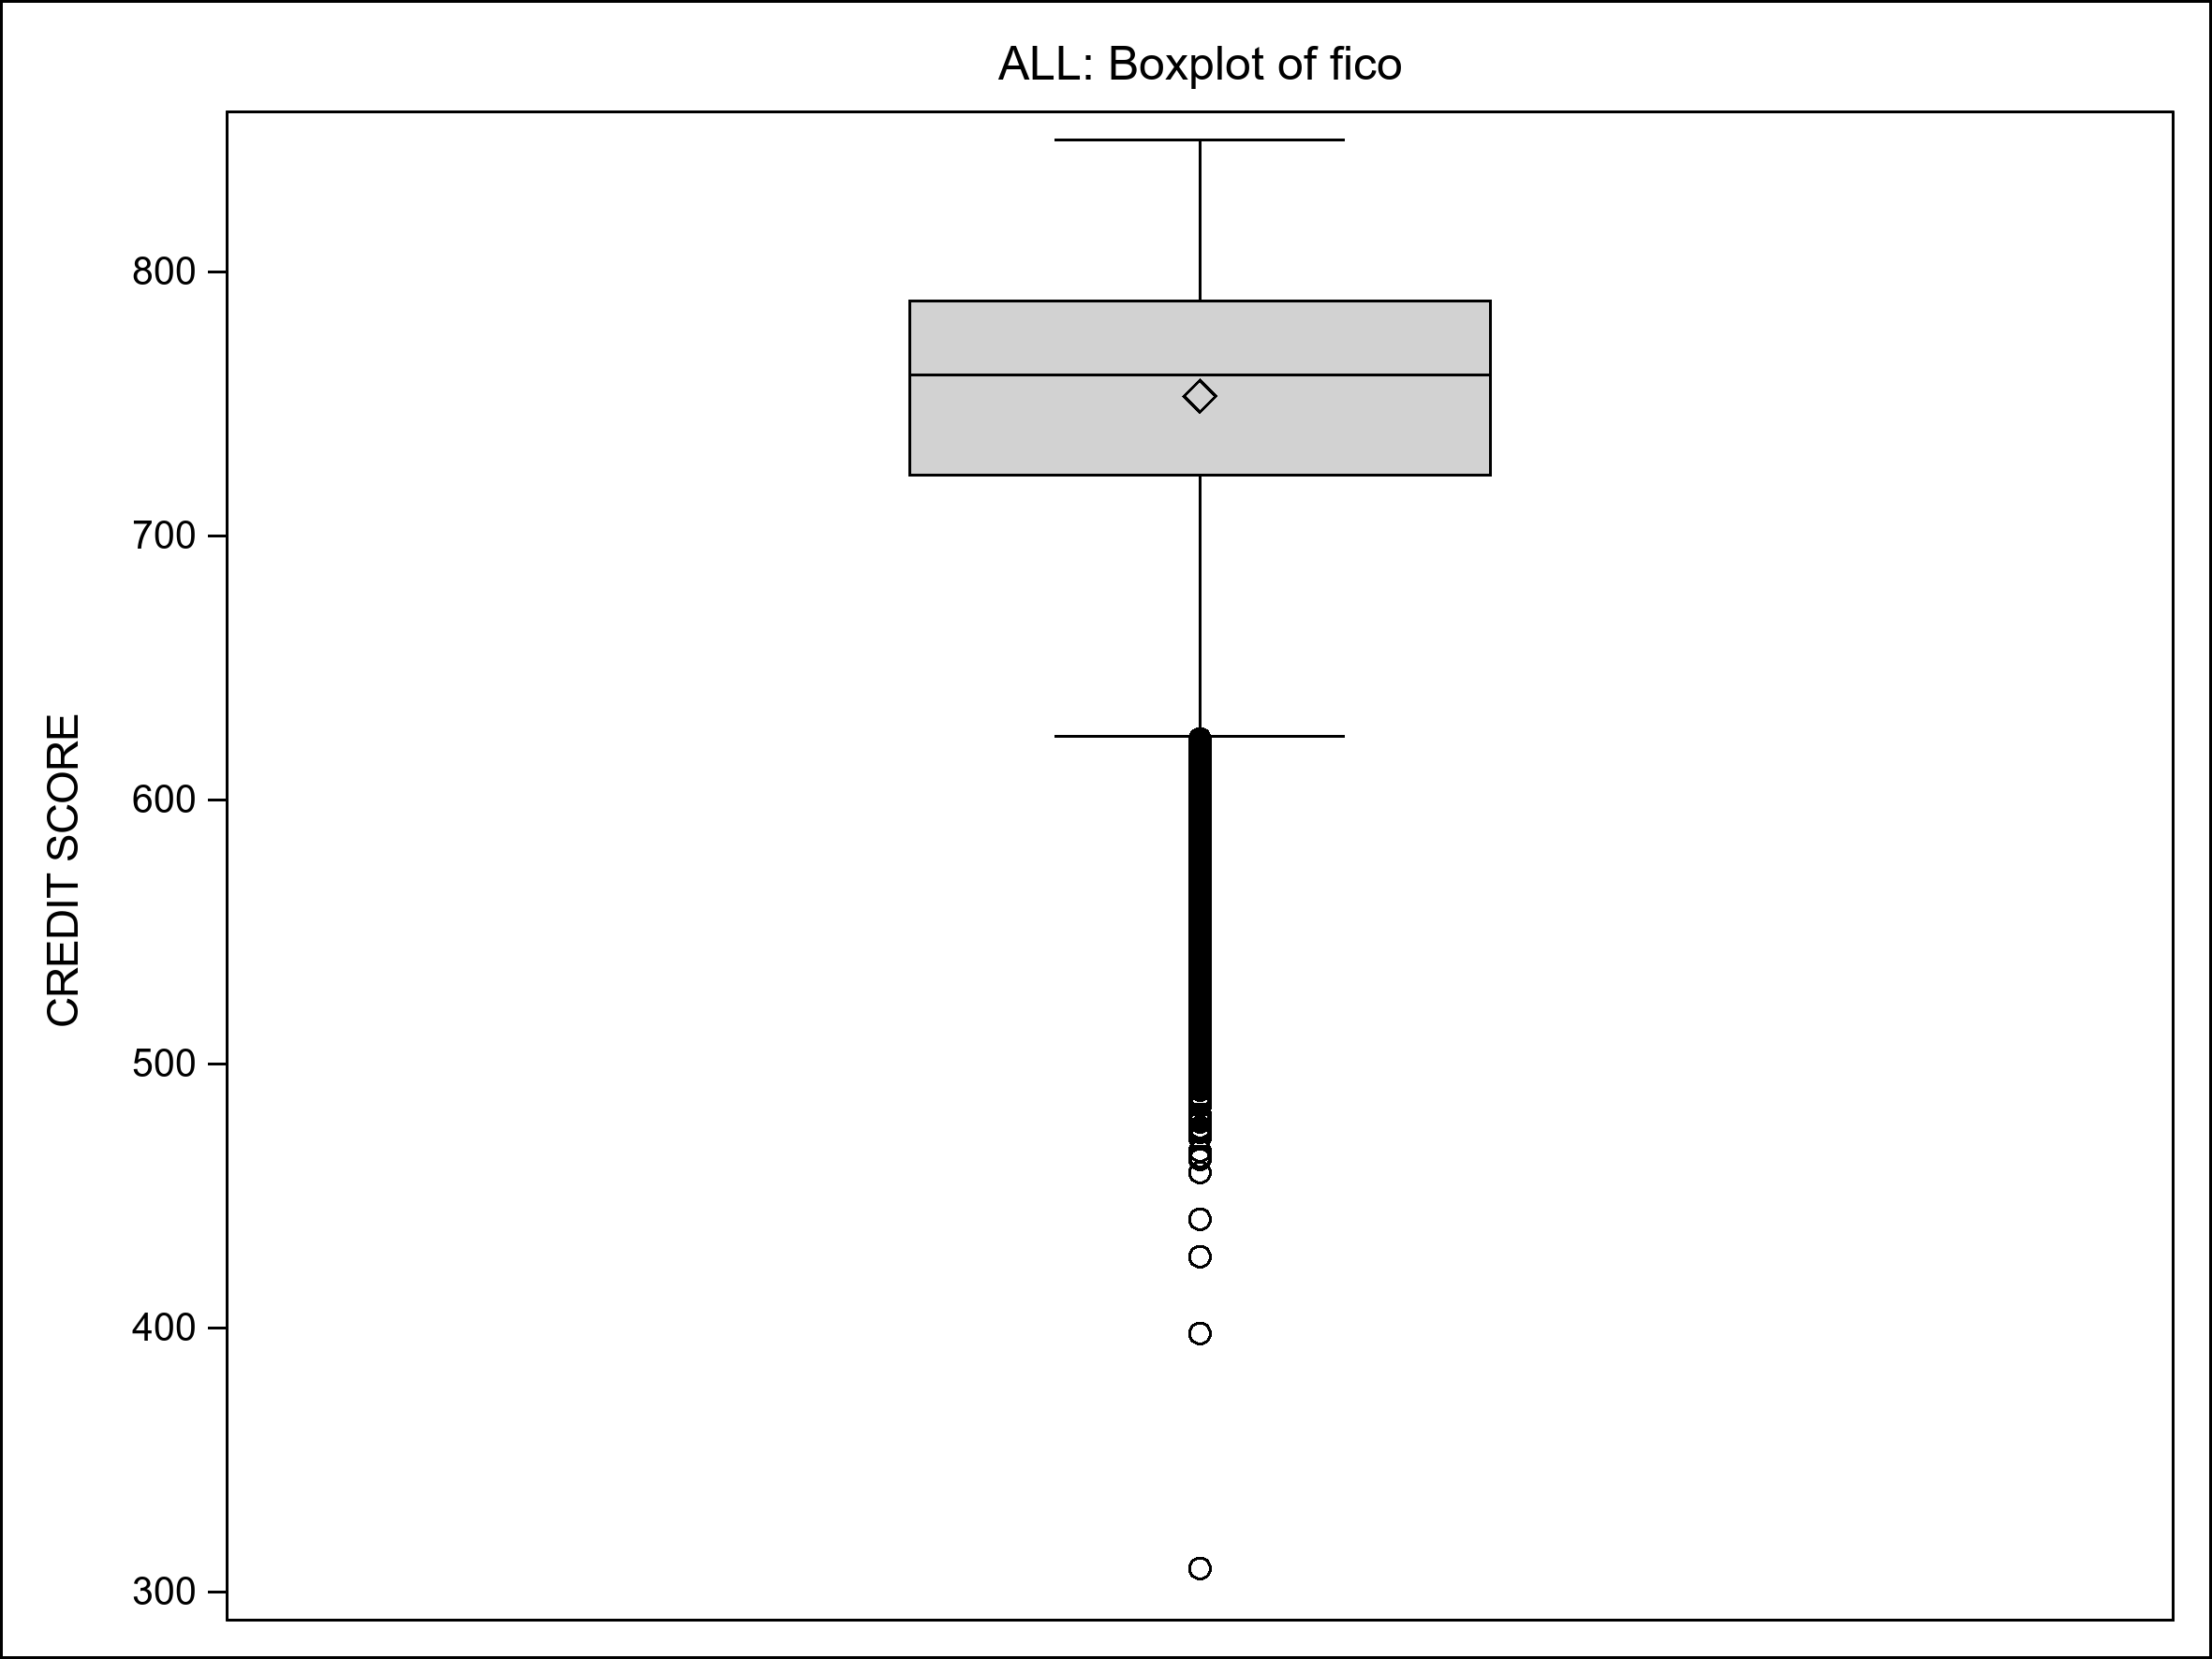
\includegraphics[width=0.9\textwidth]{./plot/Boxplot/Main/NUM_fico_BOXPLOT_ALL1.png}
\end{minipage}%
\begin{minipage}{.5\textwidth}
	\centering
	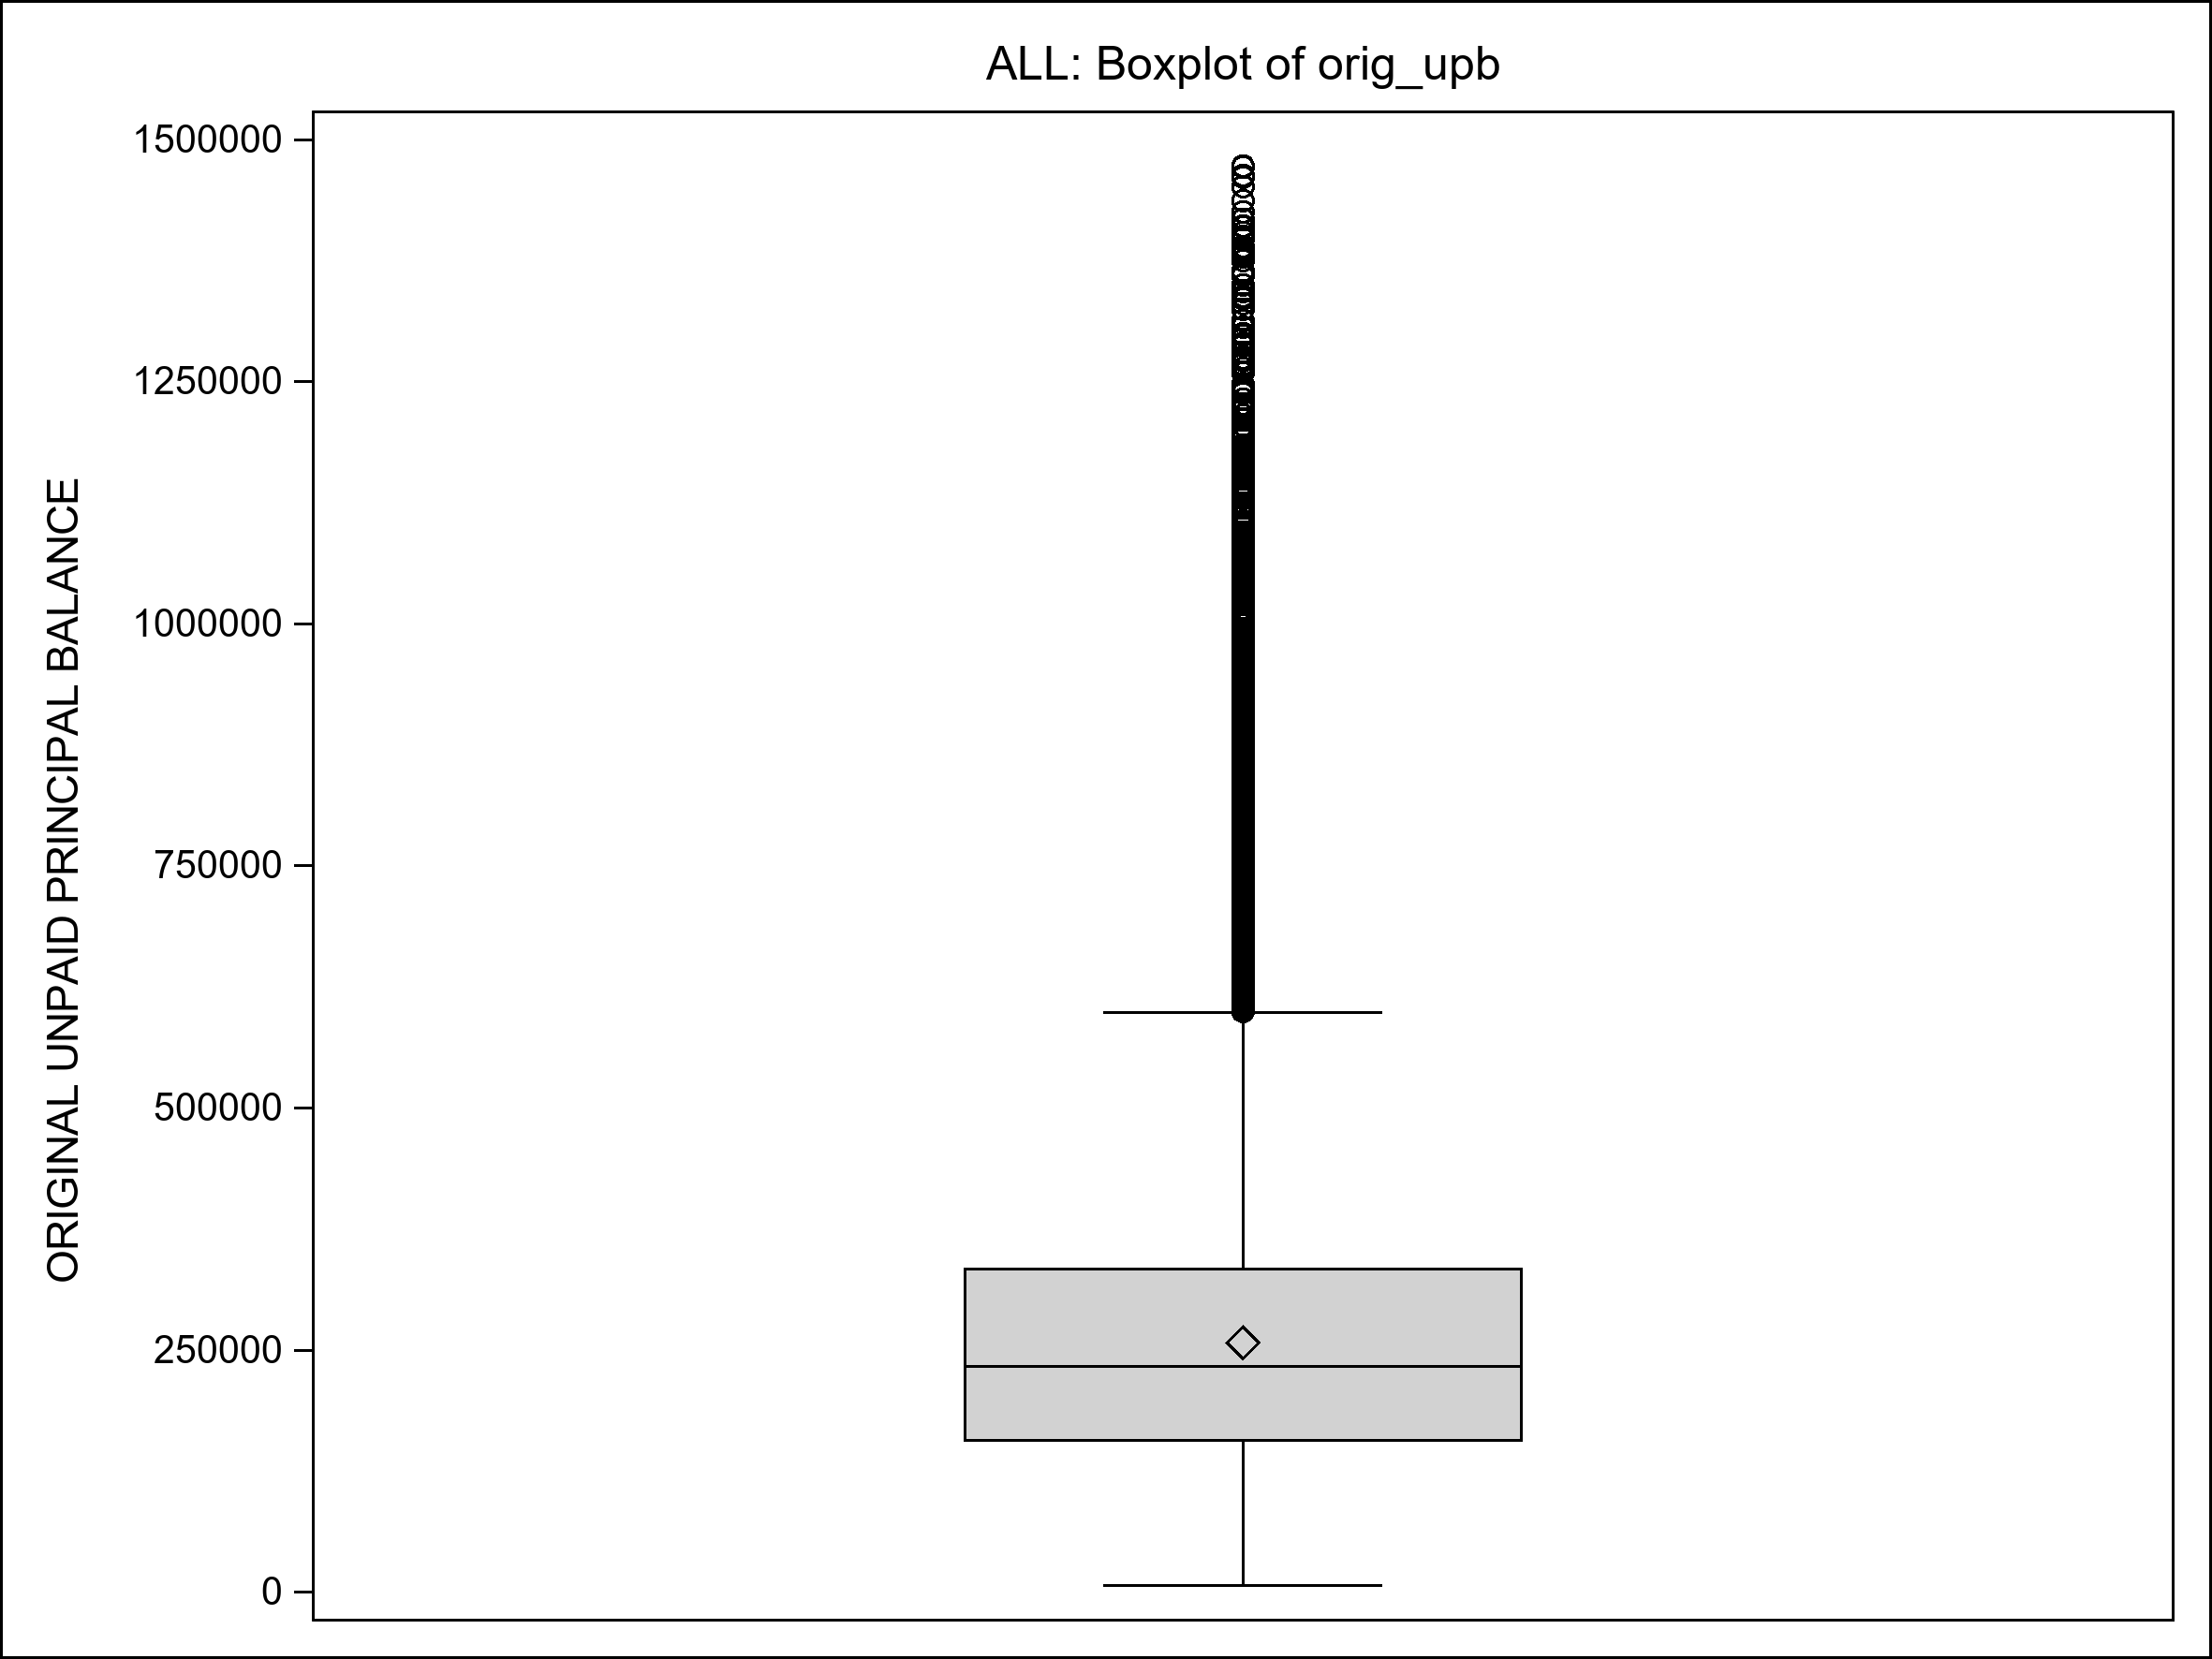
\includegraphics[width=0.9\textwidth]{./plot/Boxplot/Main/NUM_orig_upb_BOXPLOT_ALL1.png}
\end{minipage}
    \caption{Boxplot of Credit Score and UPB}
\end{figure}

\begin{figure}[H]
\begin{minipage}{.5\textwidth}
	\centering
	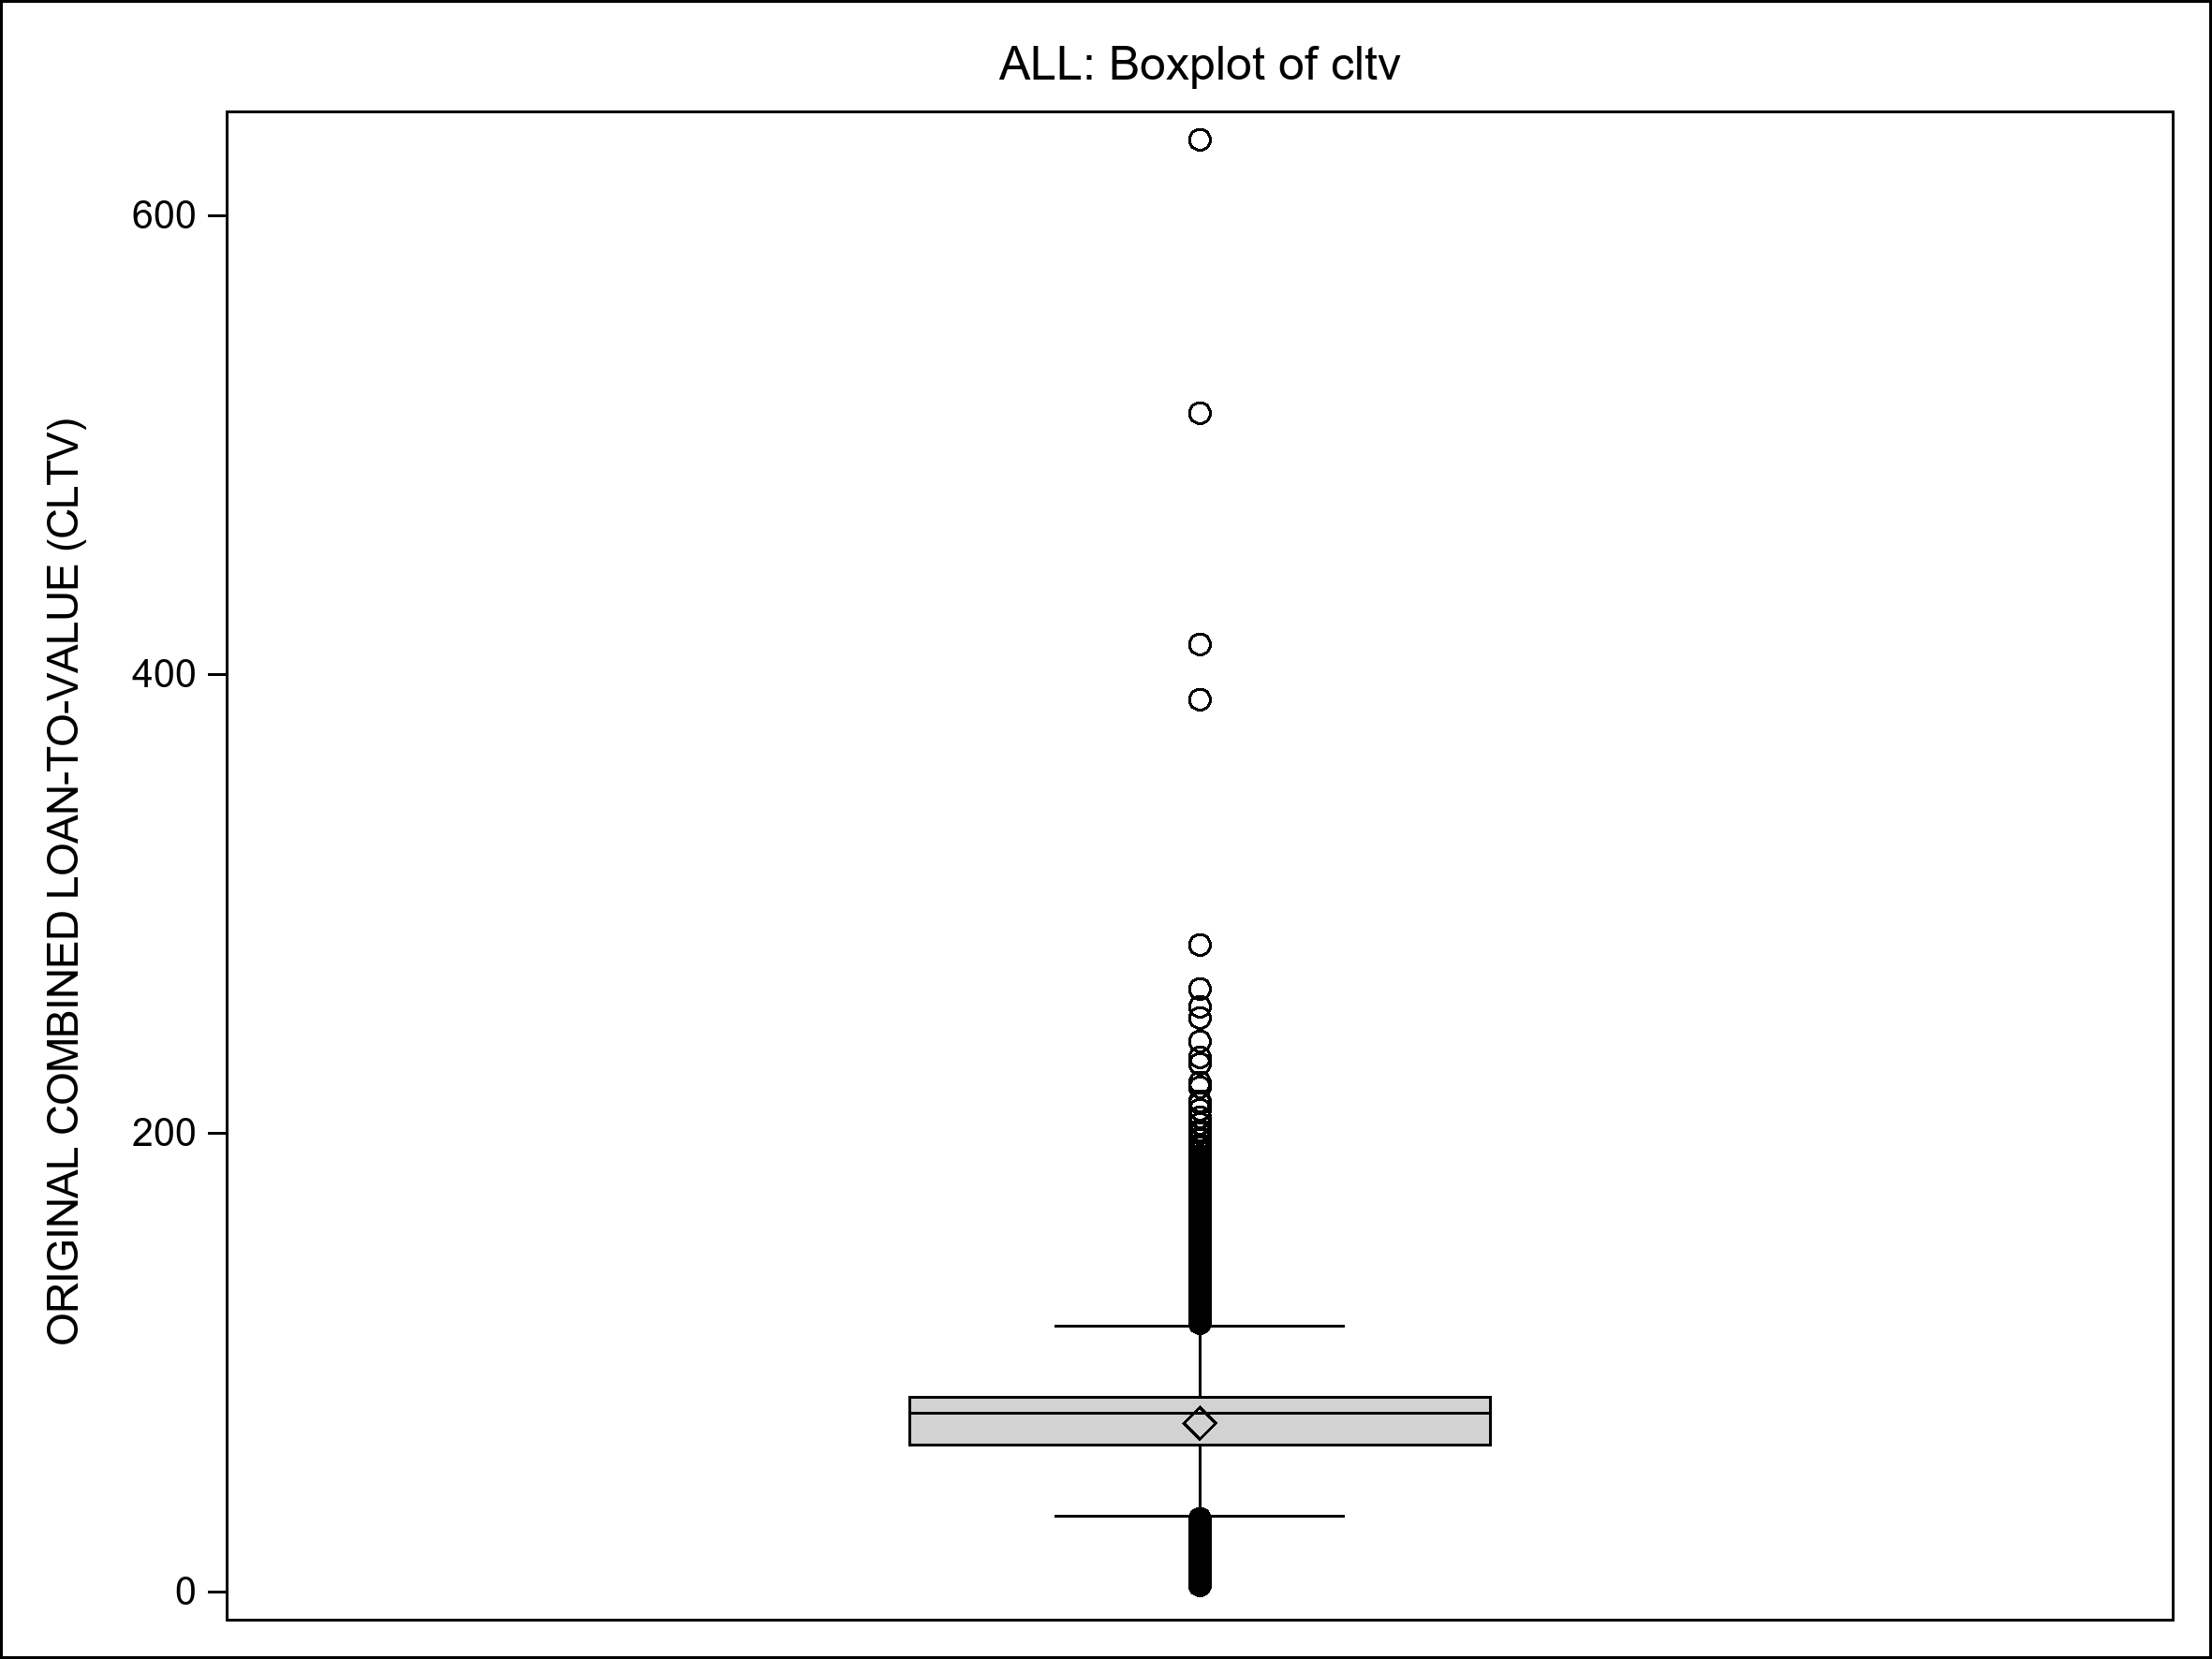
\includegraphics[width=0.9\textwidth]{./plot/Boxplot/Main/NUM_cltv_BOXPLOT_ALL1.png}
\end{minipage}%
\begin{minipage}{.5\textwidth}
	\centering
	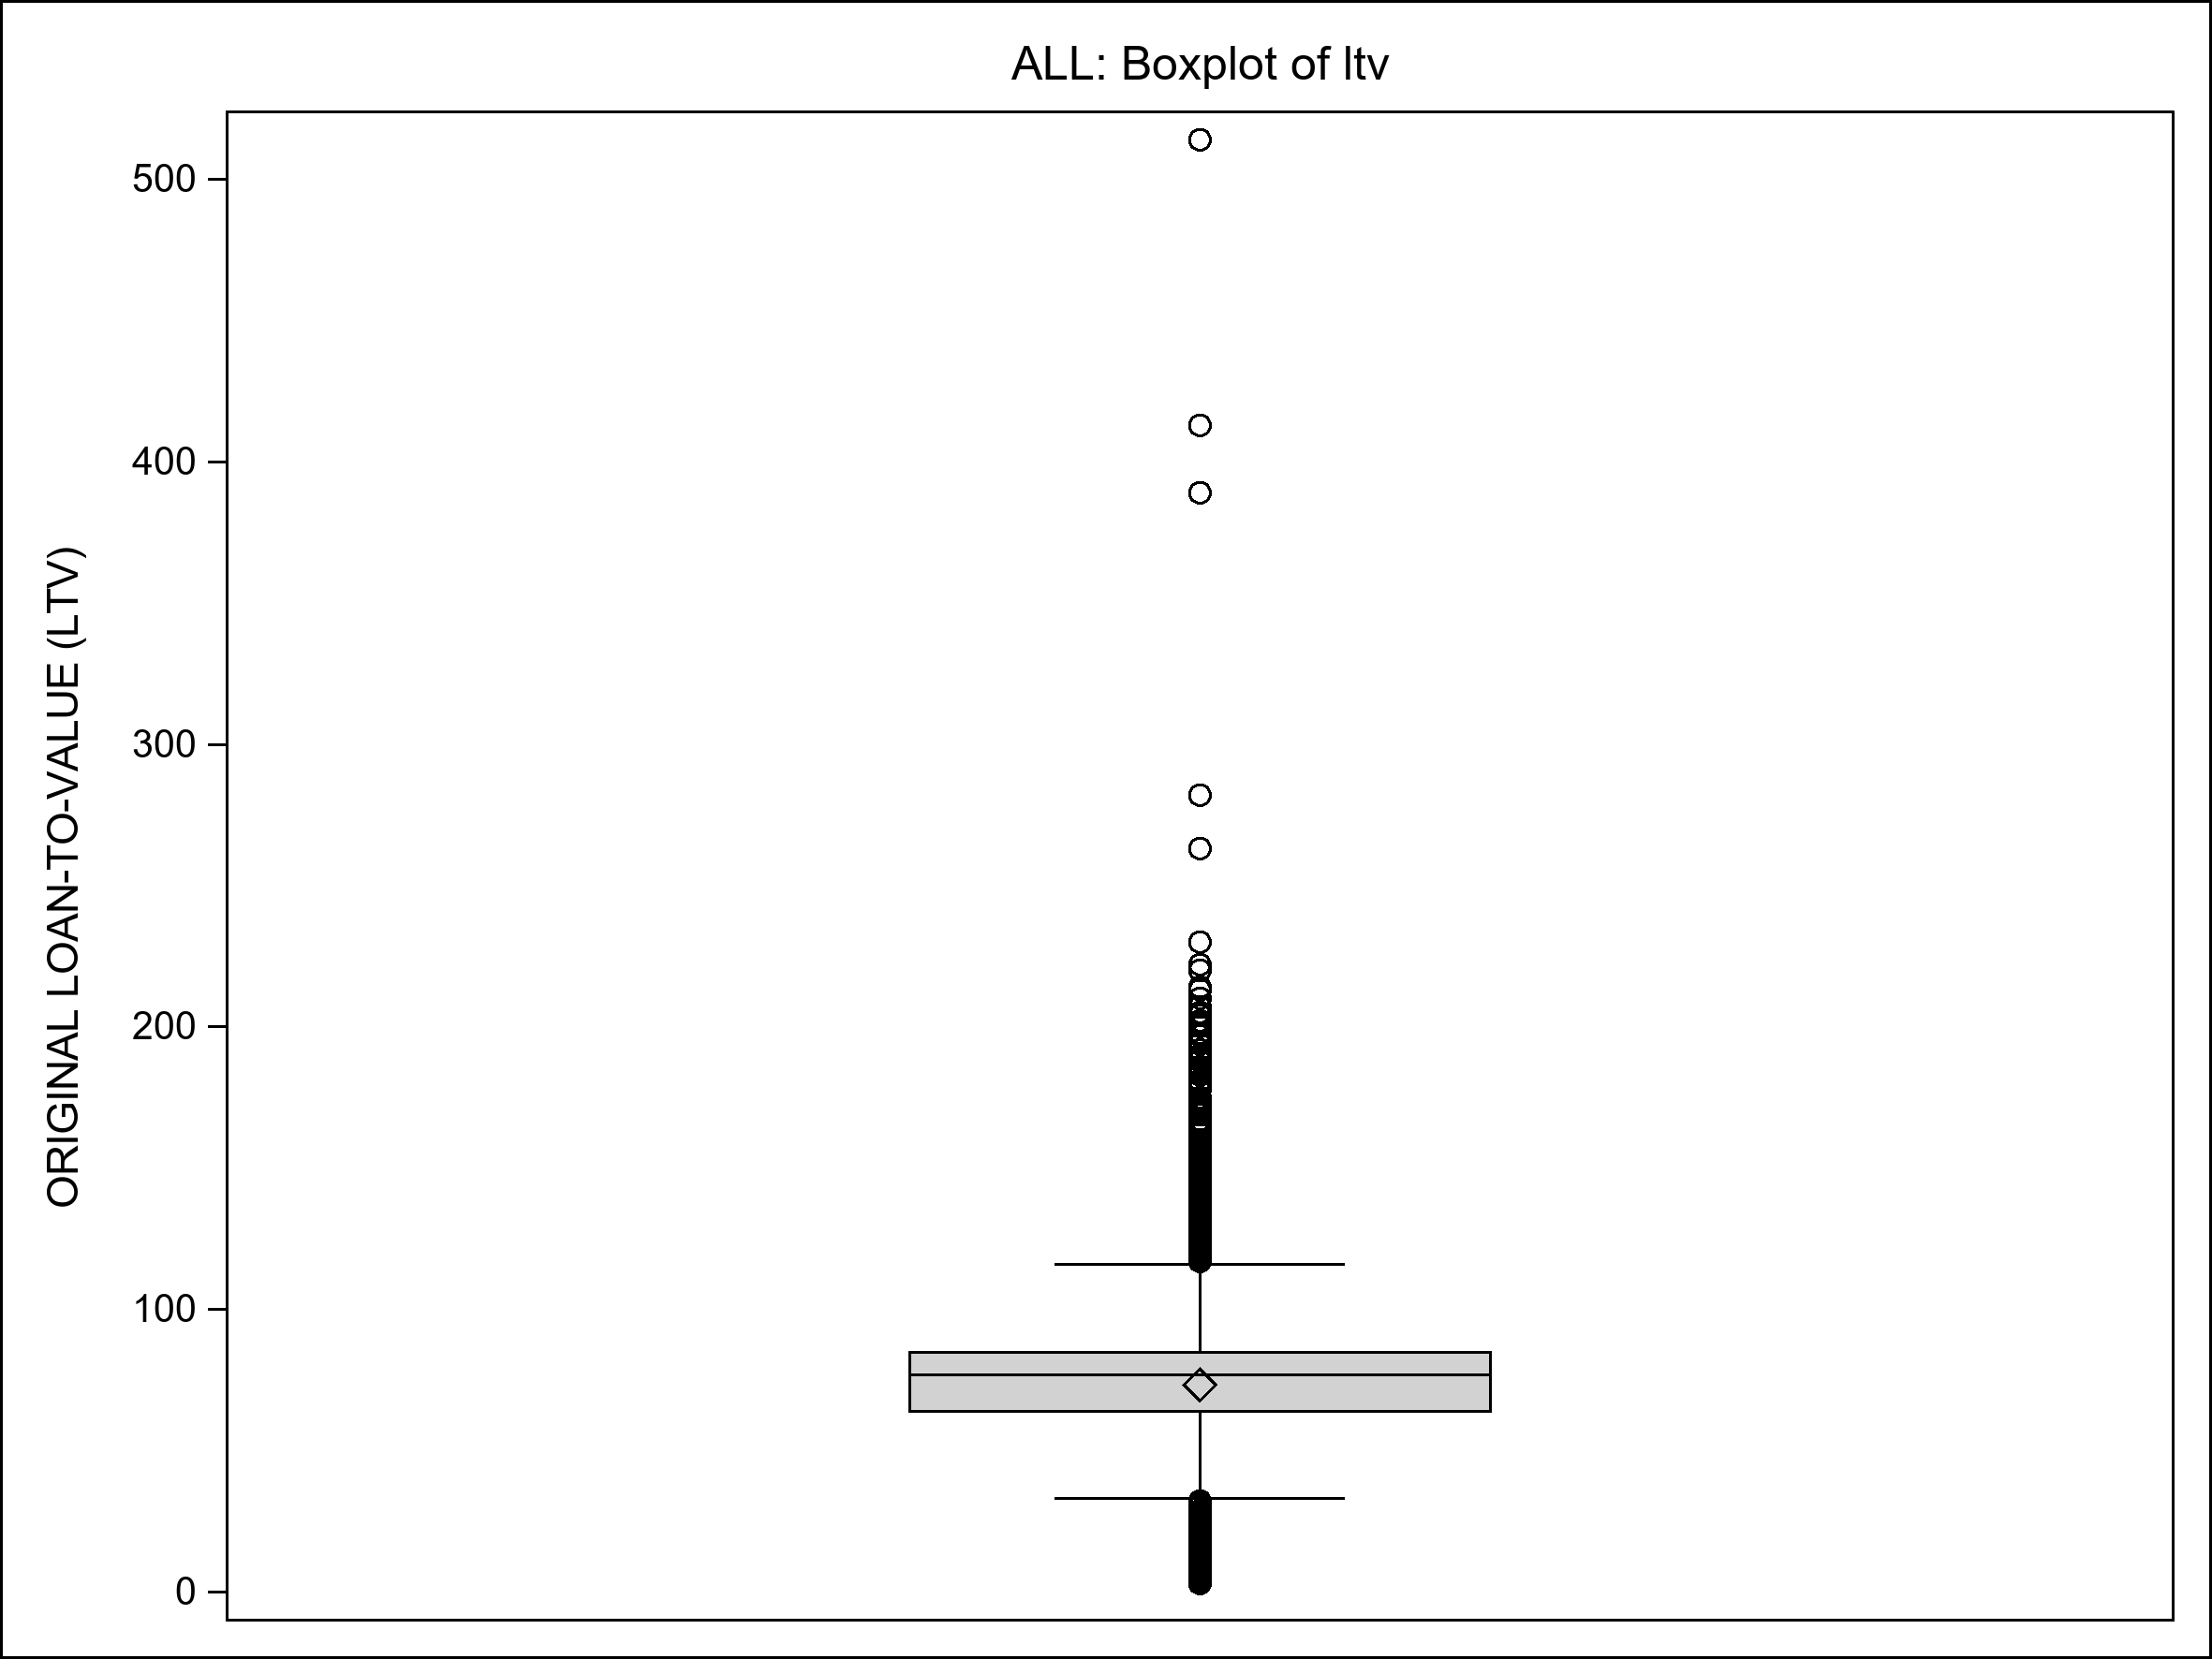
\includegraphics[width=0.9\textwidth]{./plot/Boxplot/NUM_ltv_BOXPLOT_ALL1.png}
\end{minipage}
    \caption{Boxplot of CLTV and LTV}
\end{figure}

\begin{figure}[H]
\begin{minipage}{.5\textwidth}
	\centering
	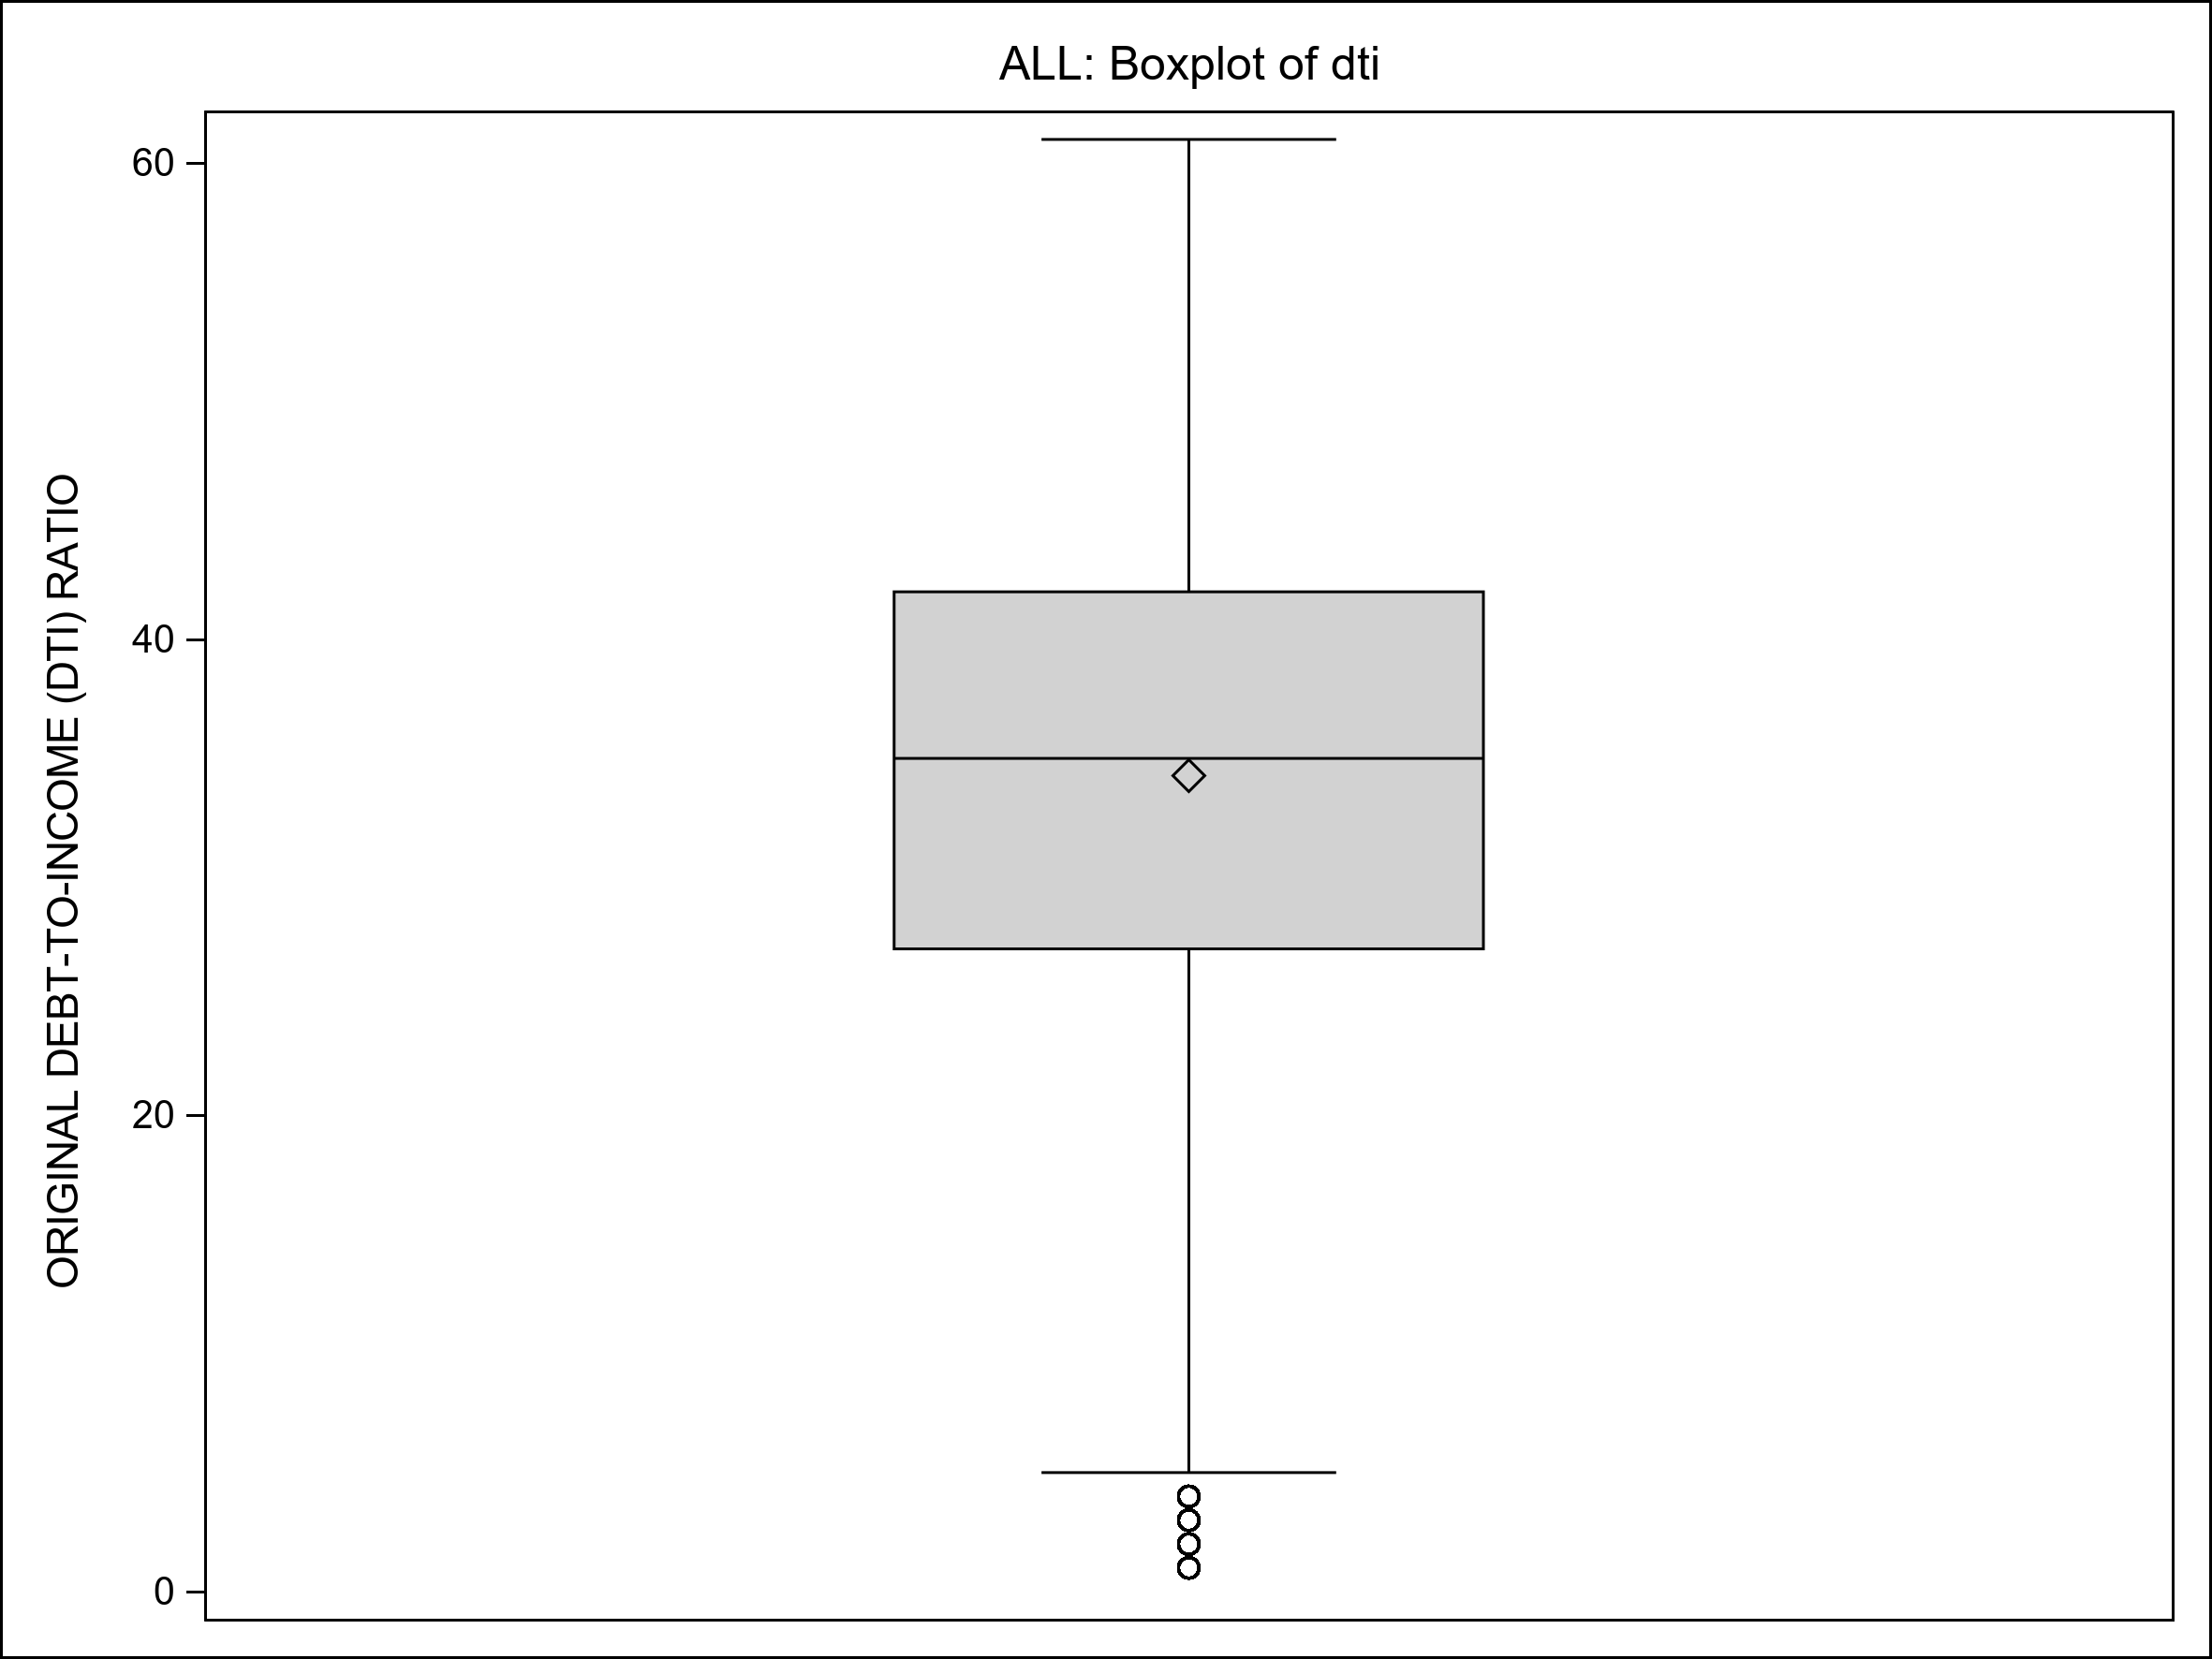
\includegraphics[width=0.9\textwidth]{./plot/Boxplot/Main/NUM_dti_BOXPLOT_ALL1.png}
\end{minipage}%
\begin{minipage}{.5\textwidth}
	\centering
	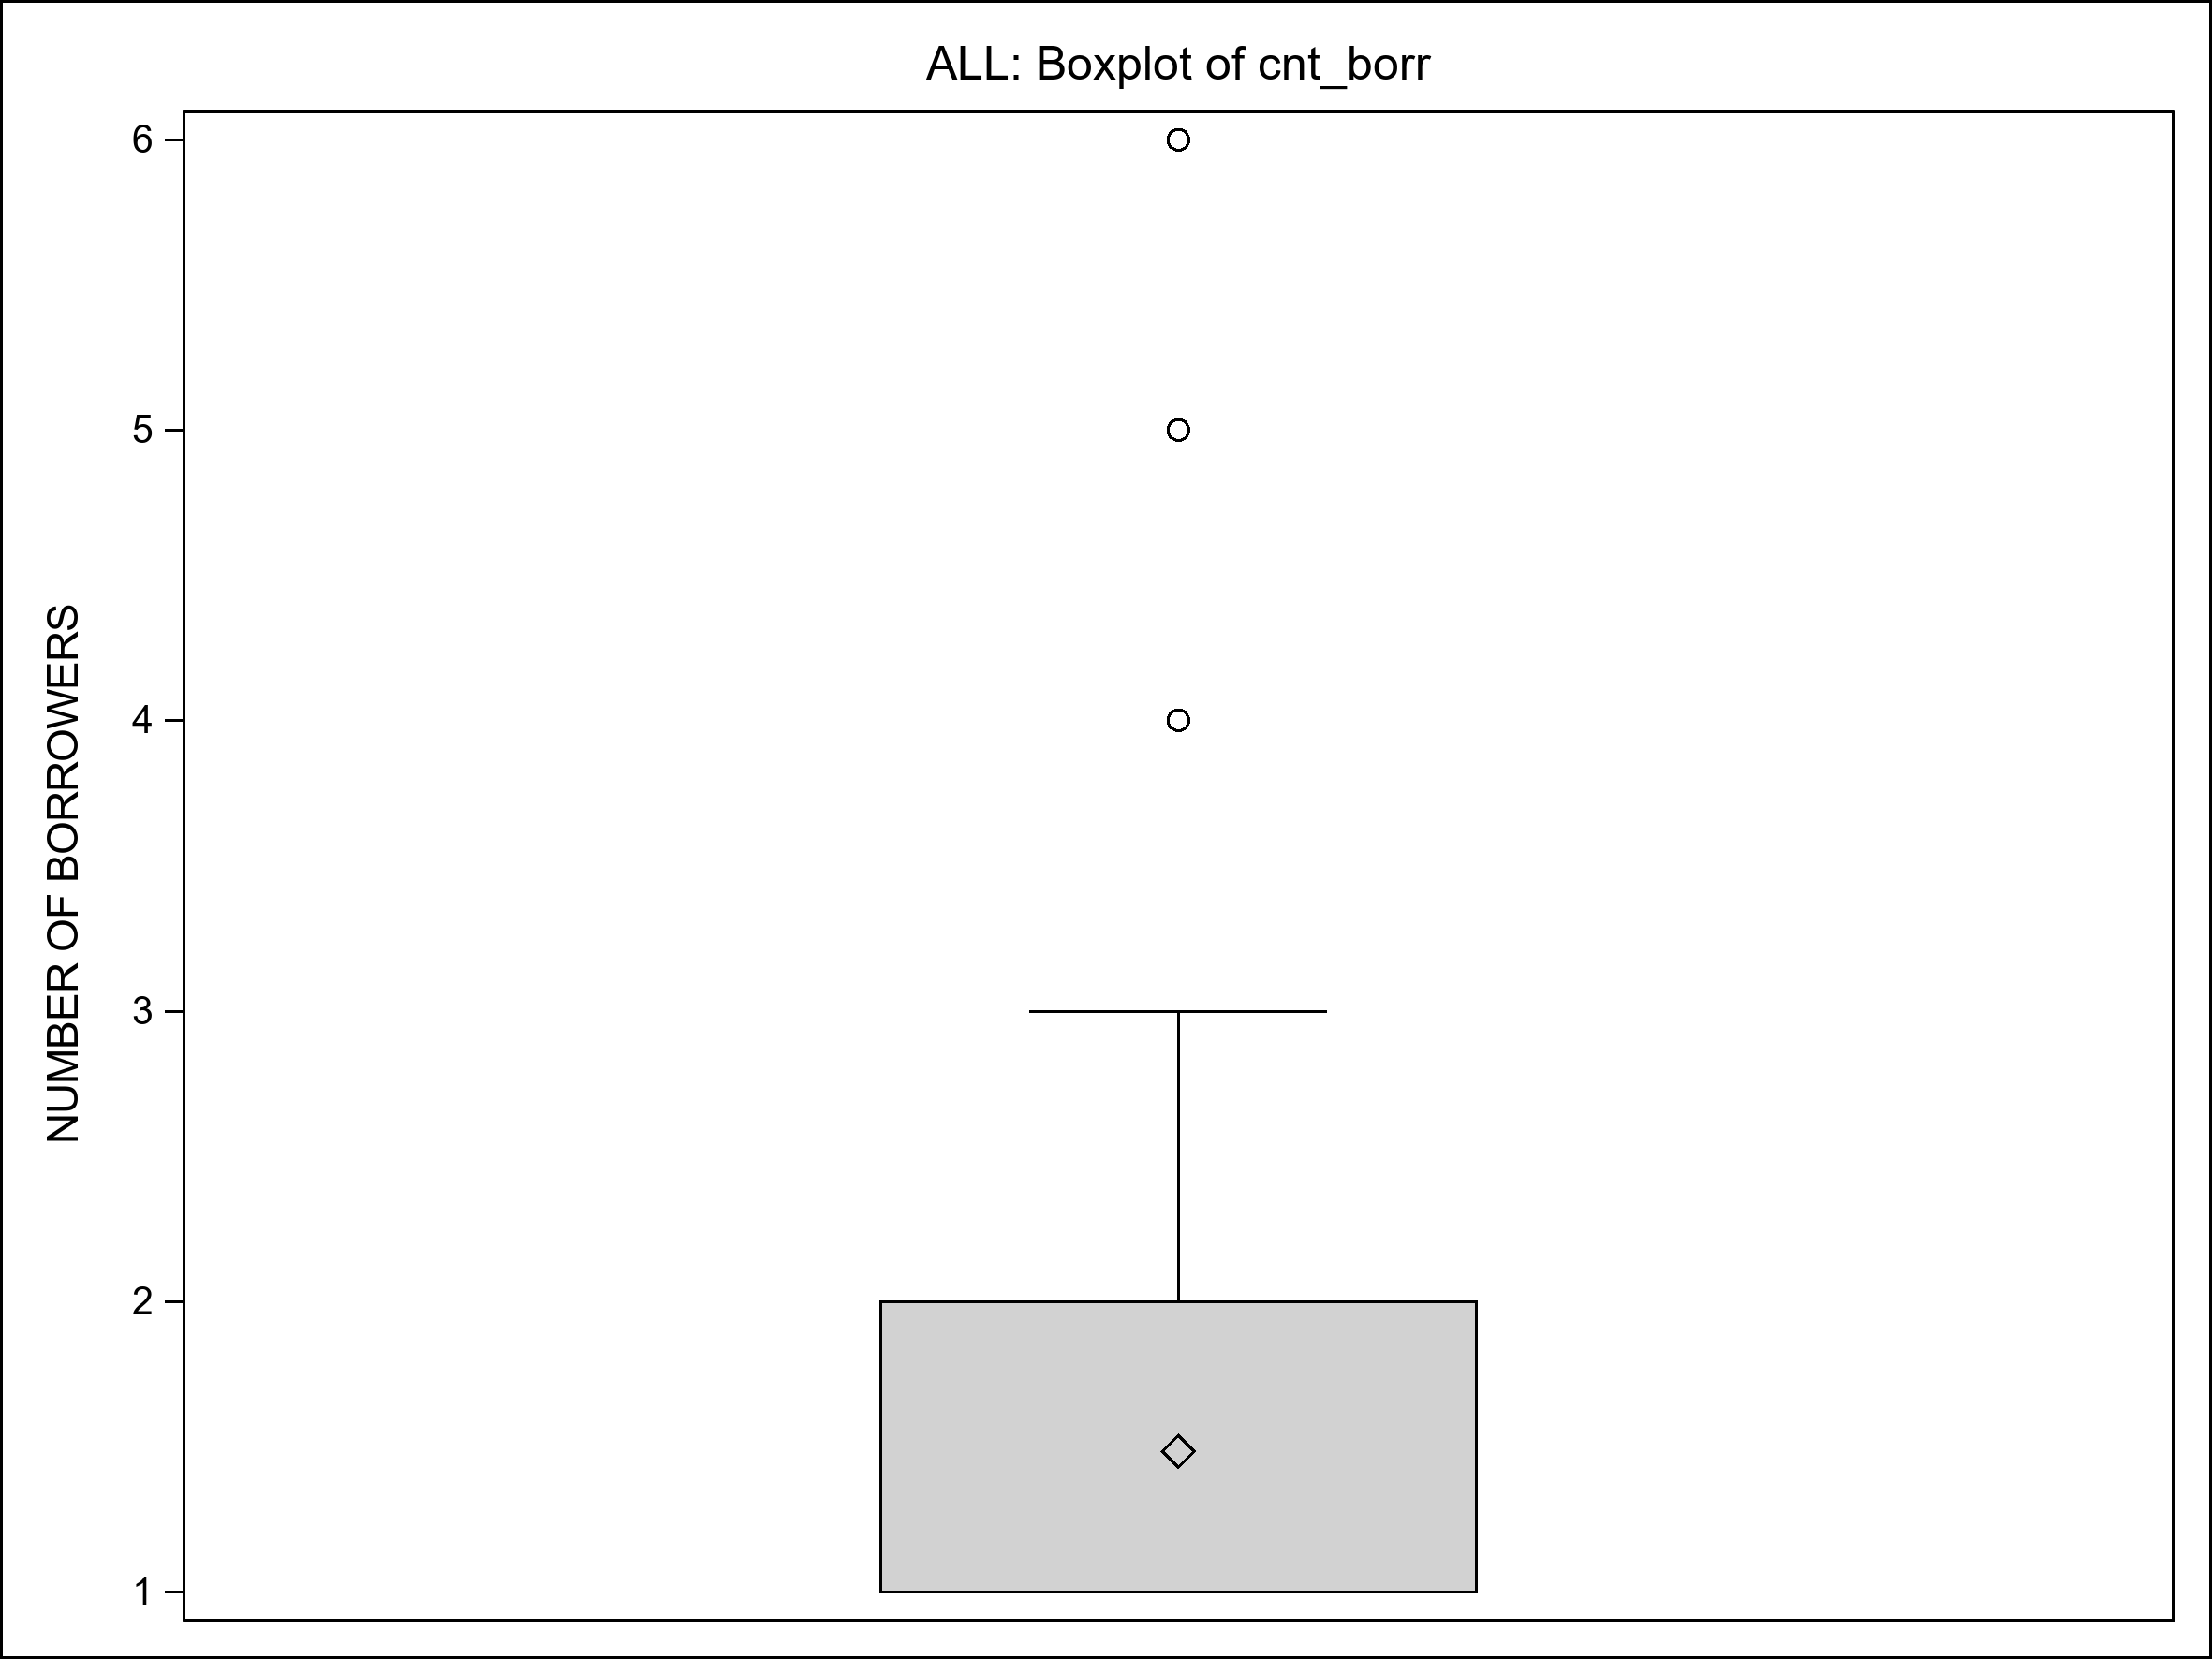
\includegraphics[width=0.9\textwidth]{./plot/Boxplot/Main/NUM_cnt_borr_BOXPLOT_ALL1.png}
\end{minipage}
    \caption{Boxplot of DTI and No Borrowers}
\end{figure}

\begin{figure}[H]
\begin{minipage}{.5\textwidth}
	\centering
	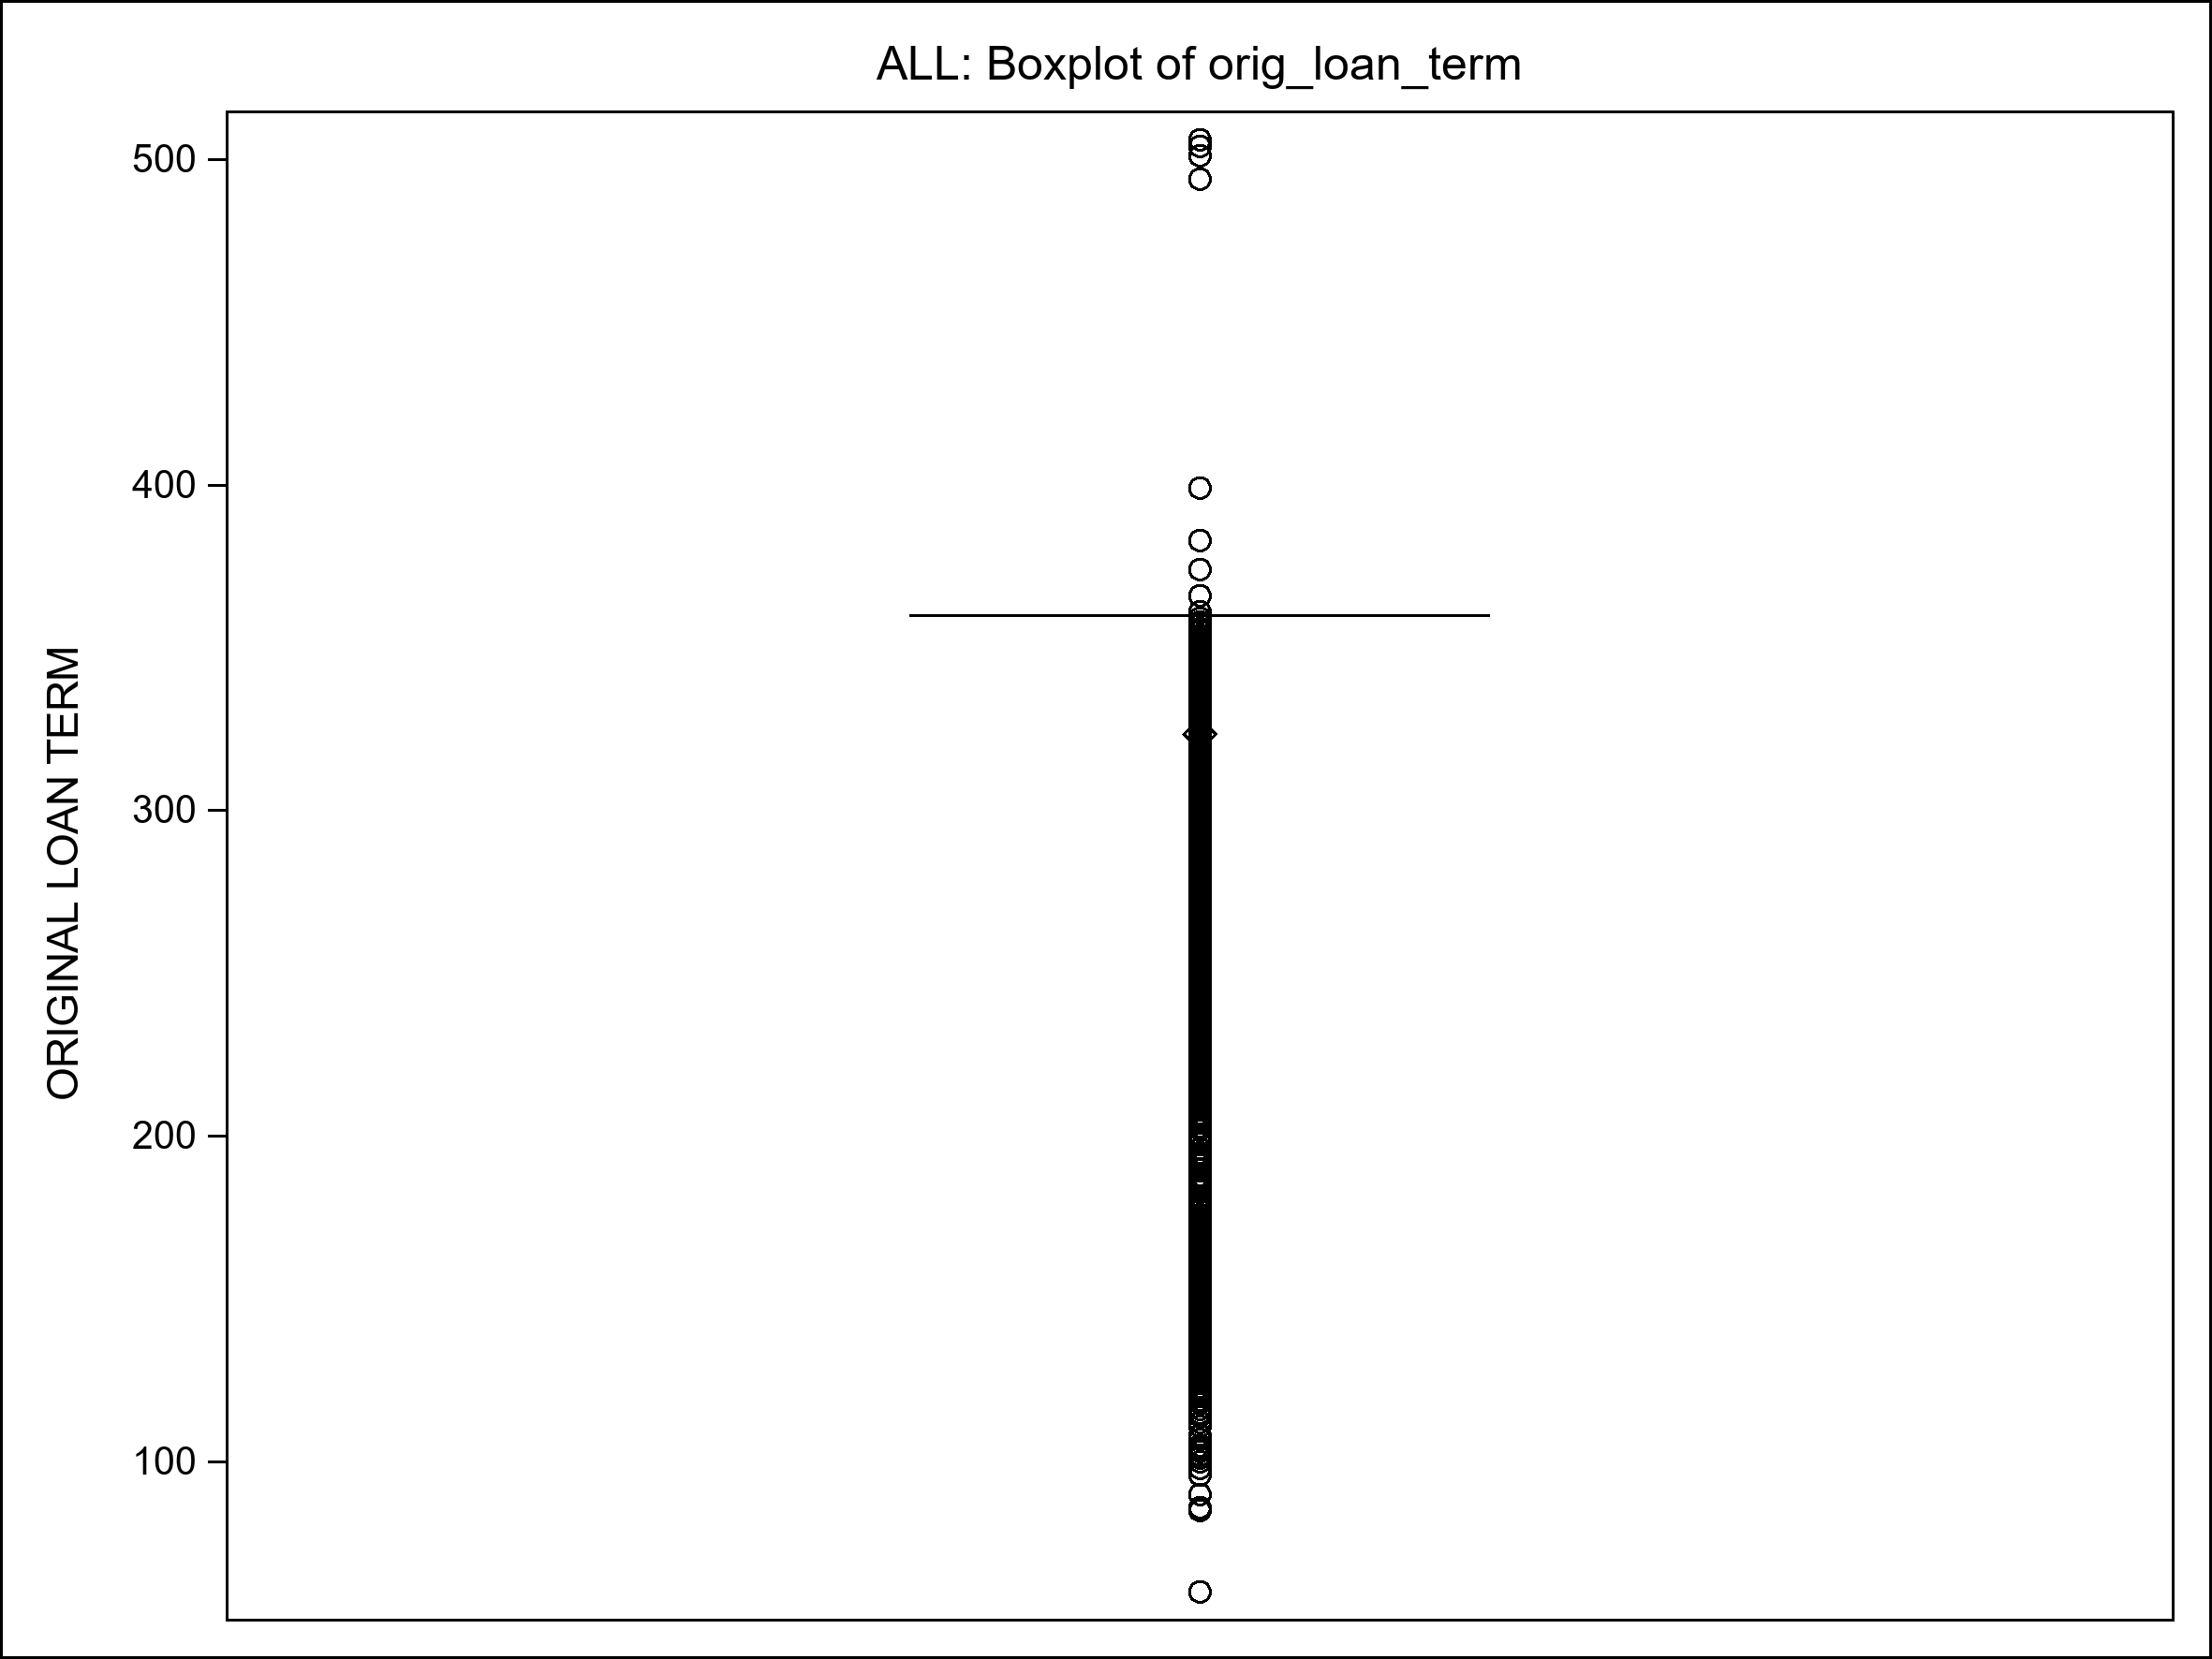
\includegraphics[width=0.9\textwidth]{./plot/Boxplot/Main/NUM_orig_loan_term_BOXPLOT_ALL1.png}
\end{minipage}%
\begin{minipage}{.5\textwidth}
	\centering
	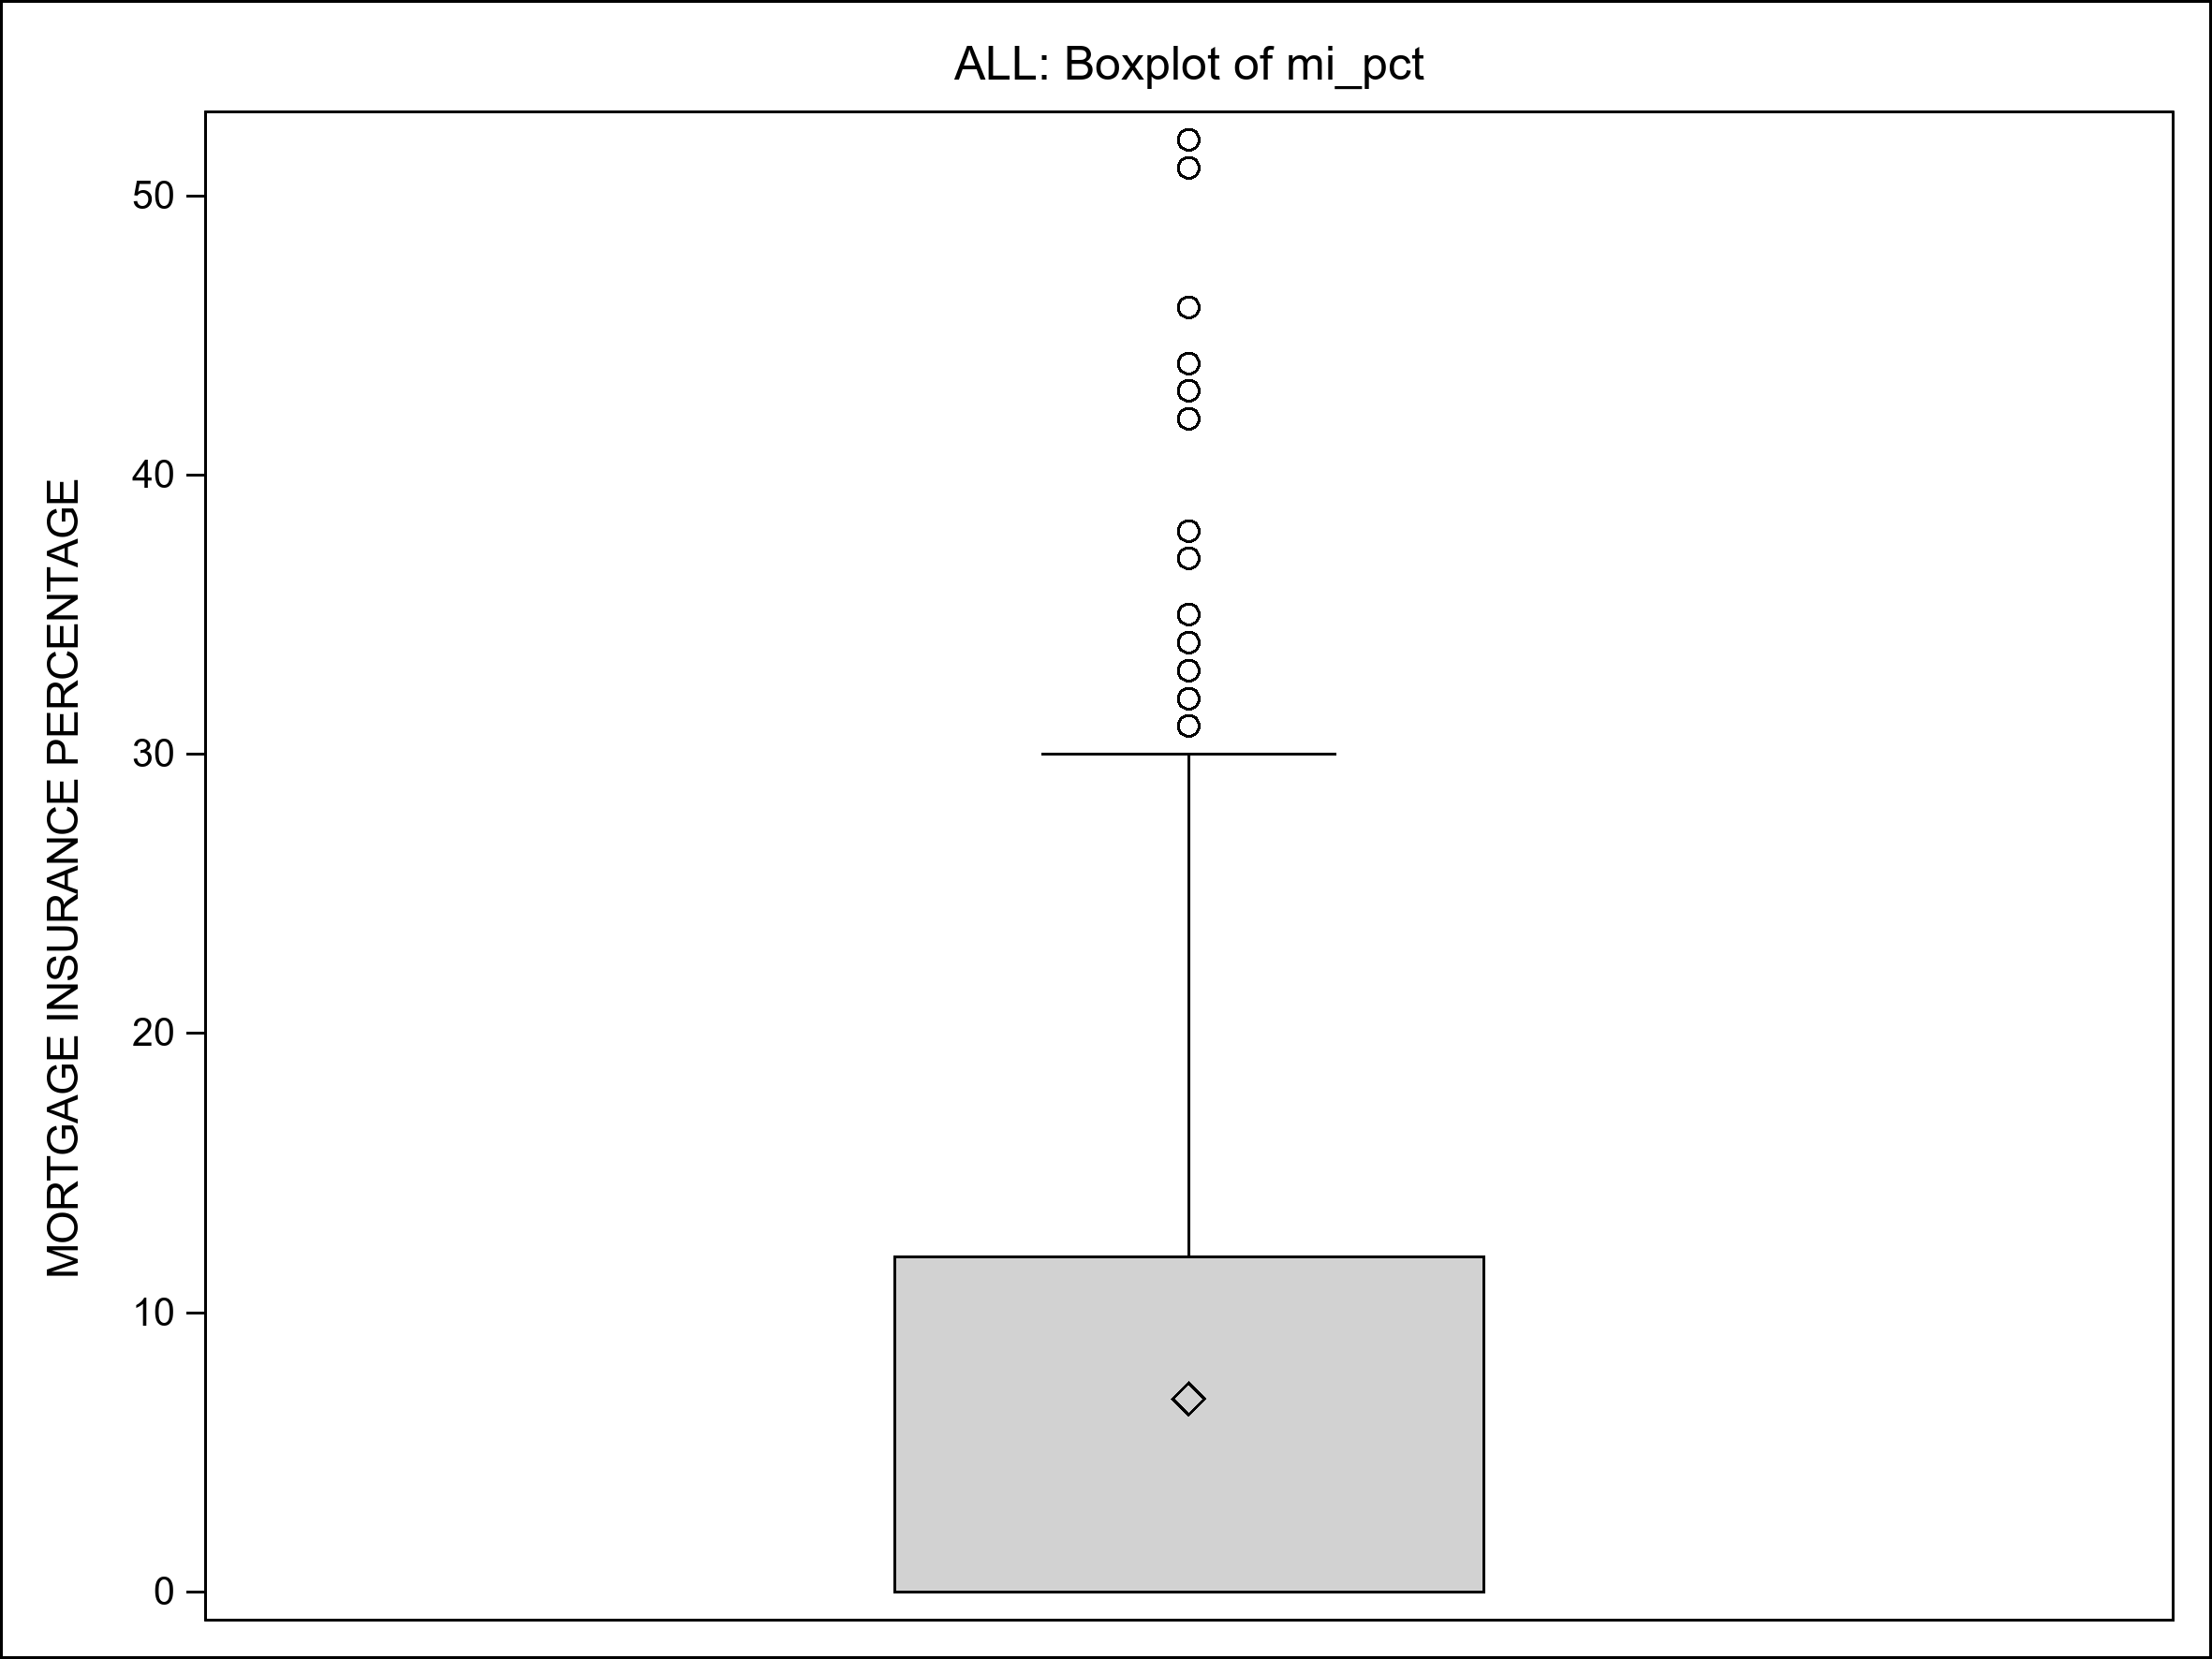
\includegraphics[width=0.9\textwidth]{./plot/Boxplot/NUM_mi_pct_BOXPLOT_ALL1.png}
\end{minipage}
    \caption{Boxplot of Loan Term and MI Perc}
\end{figure}

\begin{figure}[H]
	\centering
	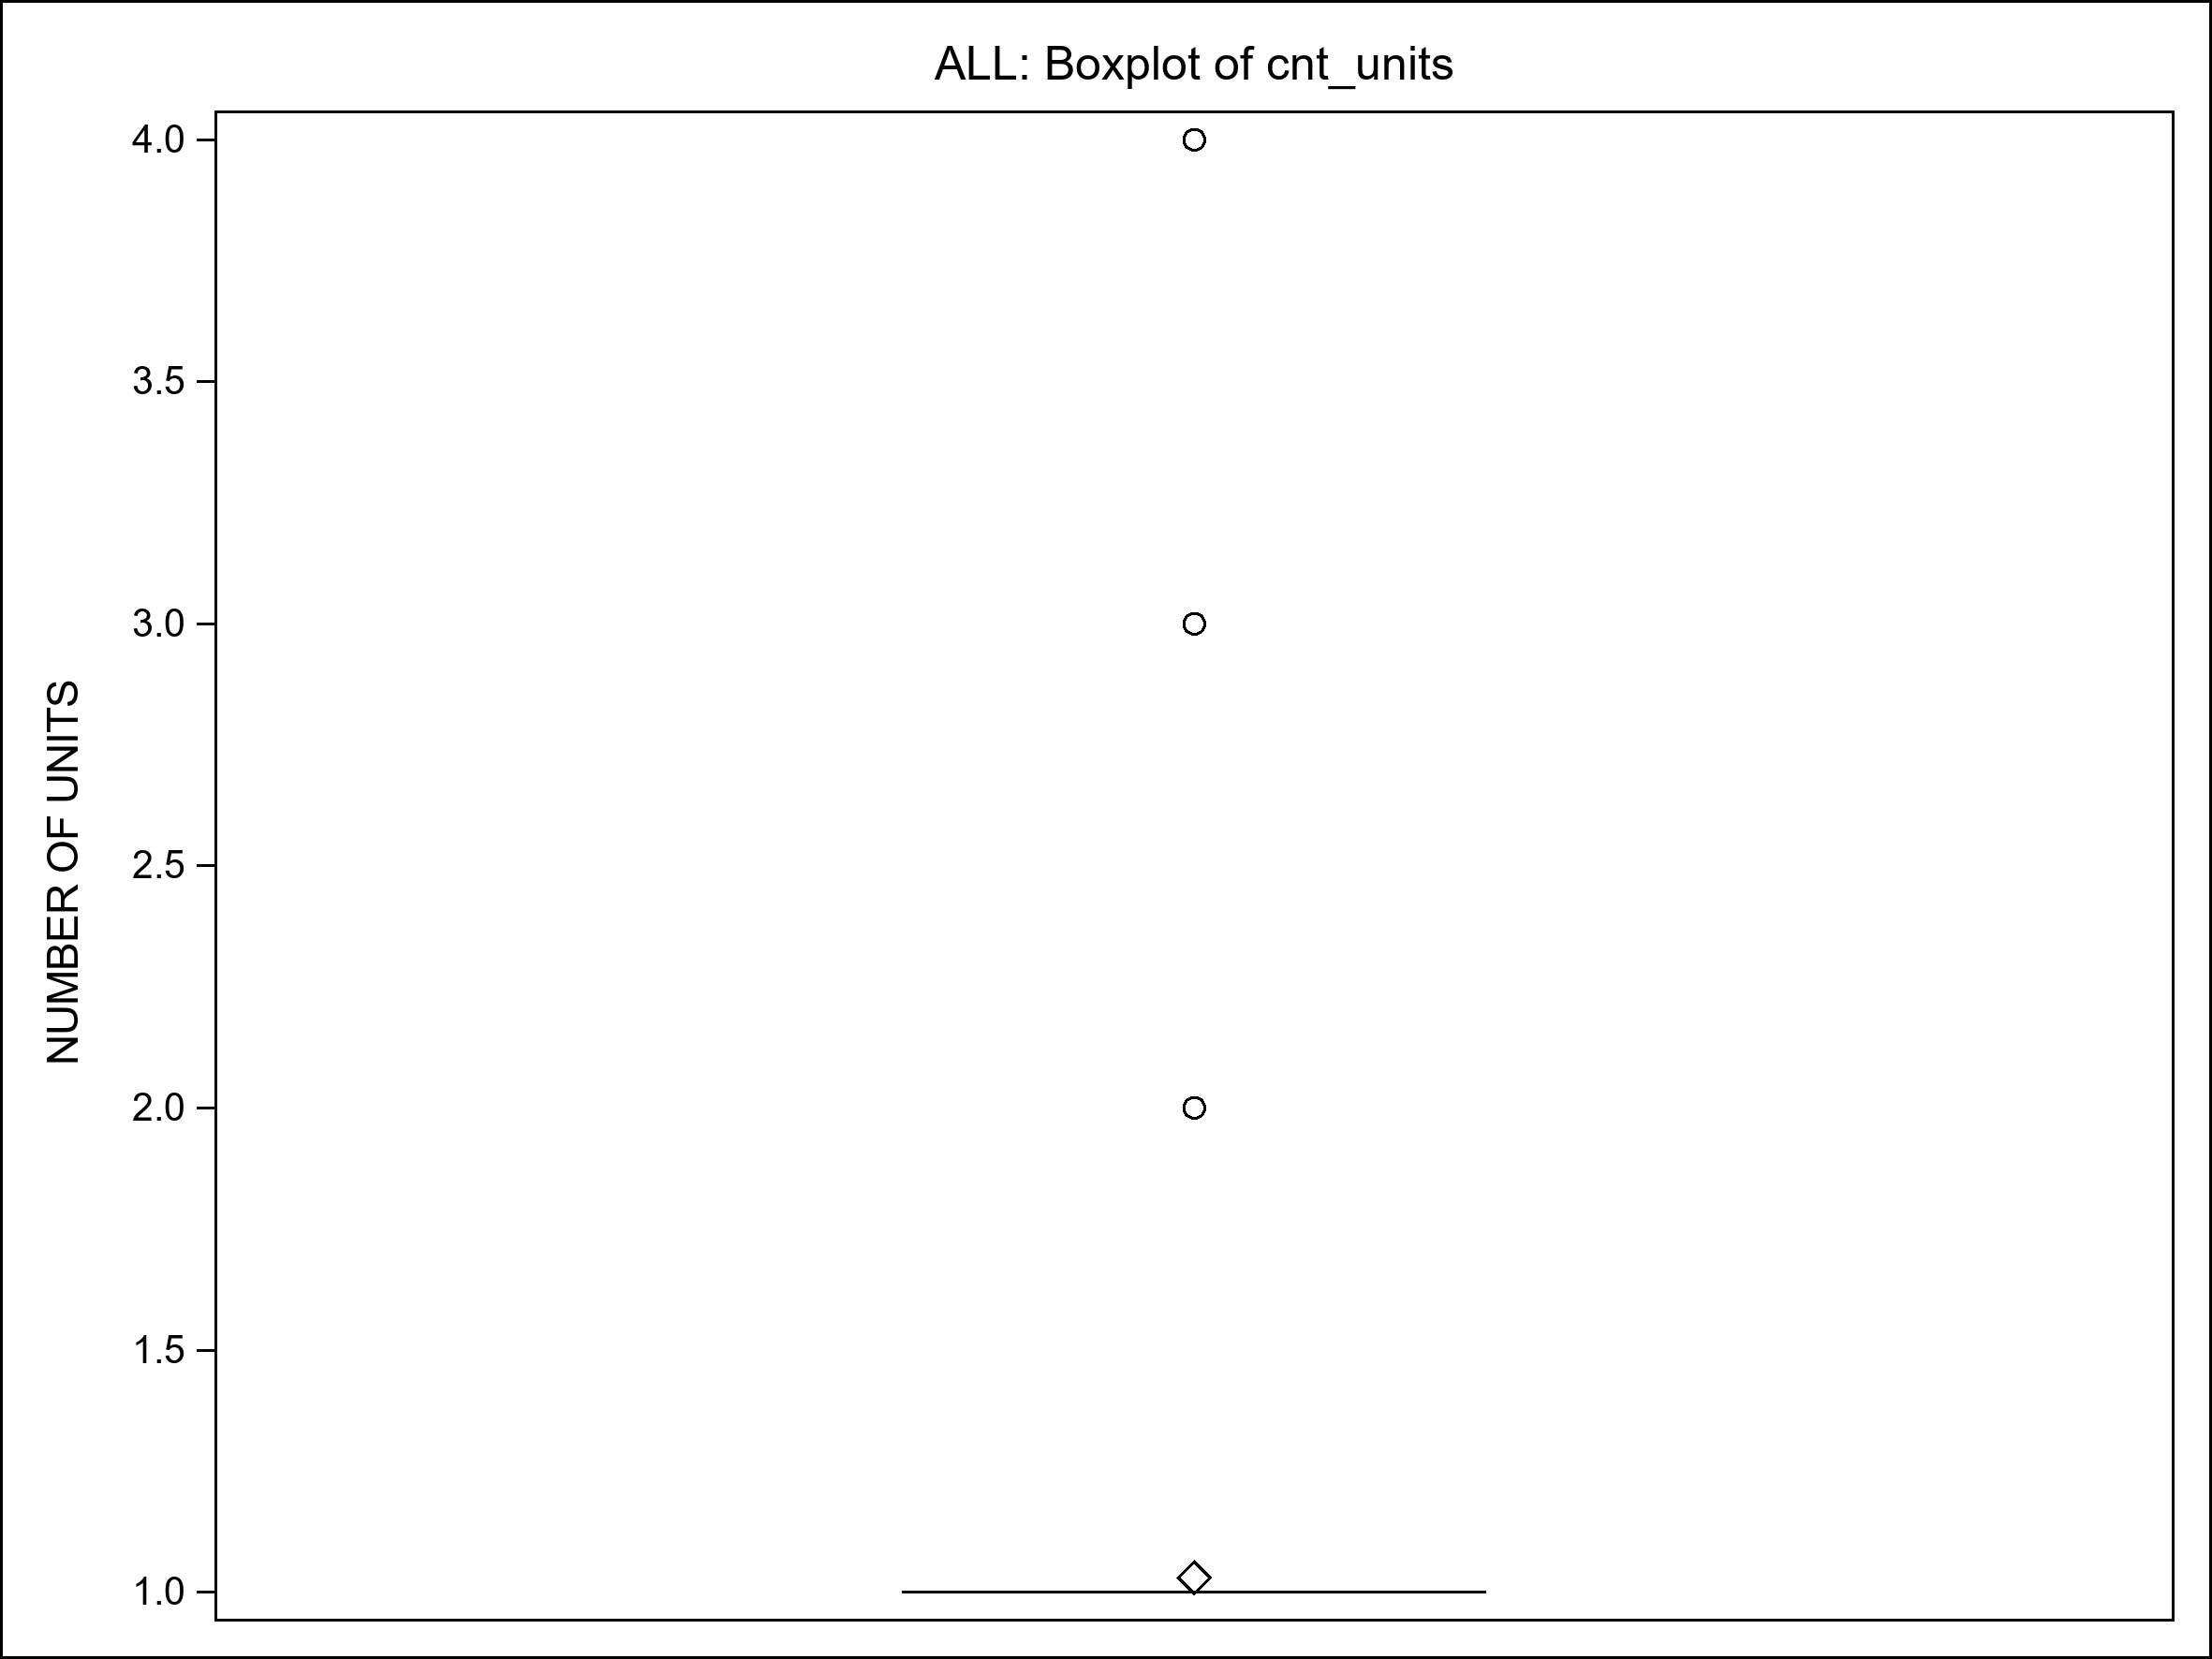
\includegraphics[width=0.5\textwidth]{./plot/Boxplot/NUM_cnt_units_BOXPLOT_ALL1.png}
    \caption{Boxplot of No Units}
\end{figure}

\section{ROC-curves of all variables}
\label{sec:ROC_all}

\subsection{Numerical variables}

\begin{figure}[H]
\begin{minipage}{.5\textwidth}
	\centering
	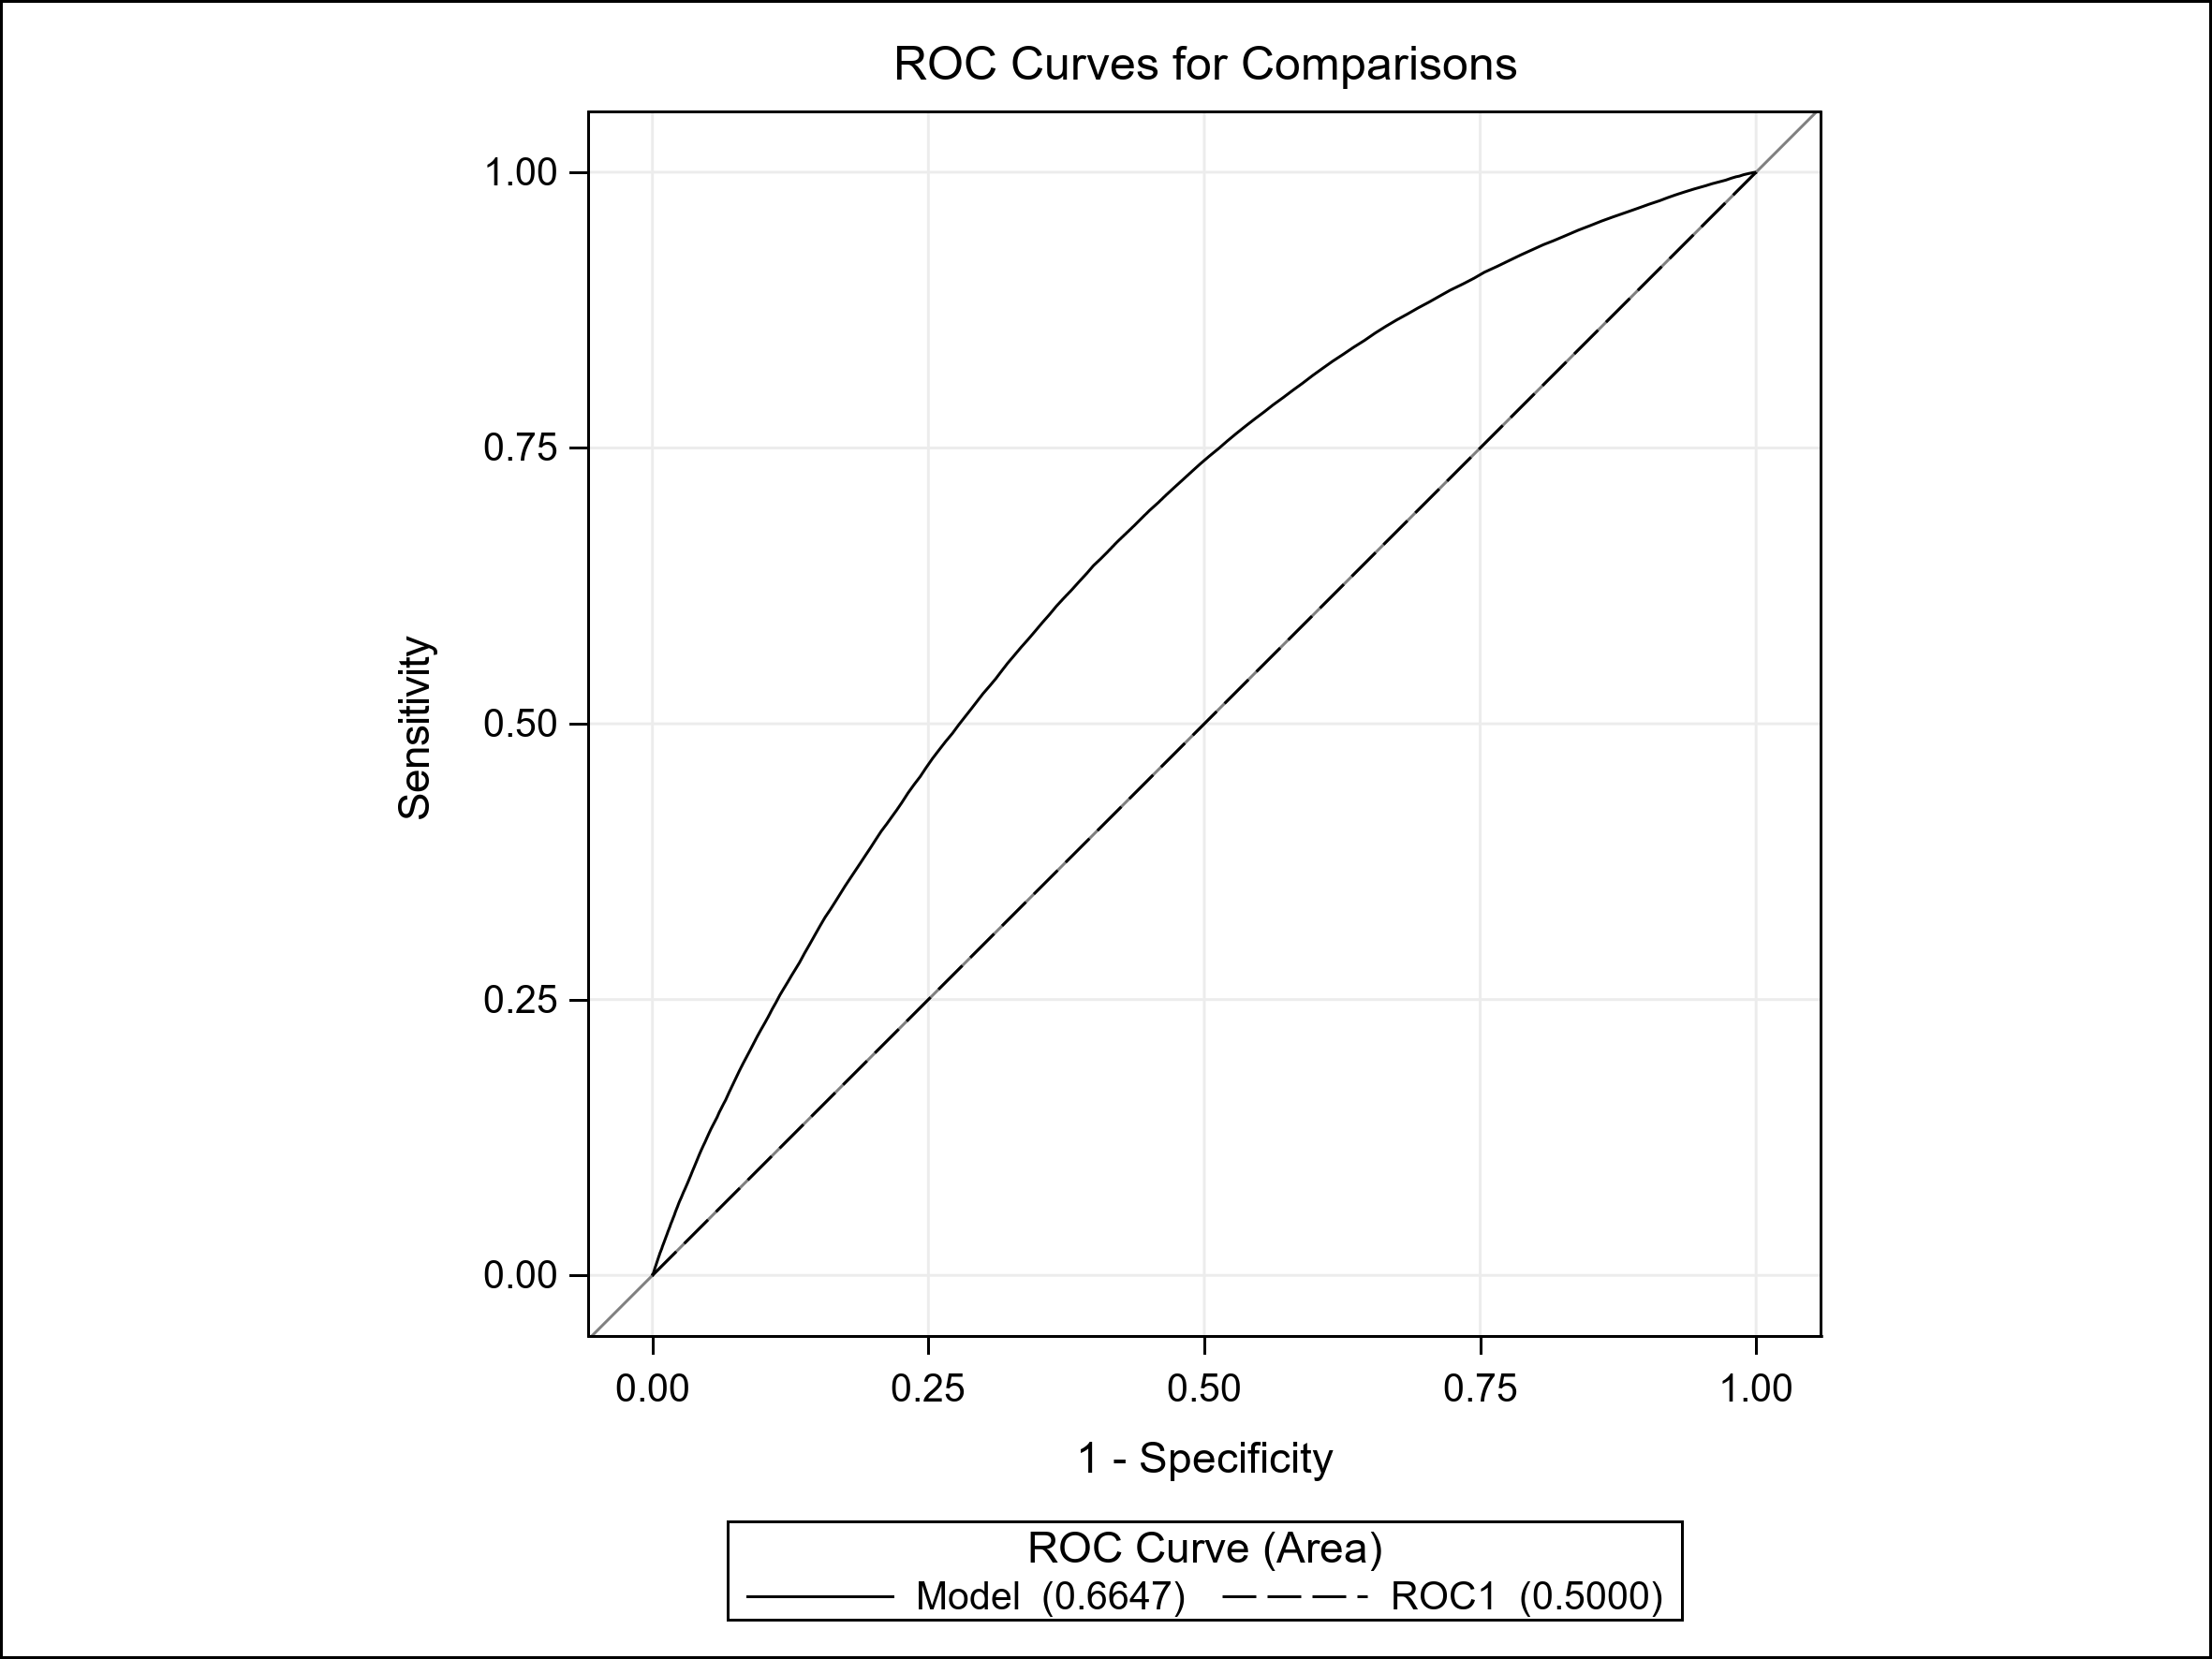
\includegraphics[width=0.9\textwidth]{./plot/ROC/Main/NUM_fico_ROC_ALL5.png}
\end{minipage}%
\begin{minipage}{.5\textwidth}
	\centering
	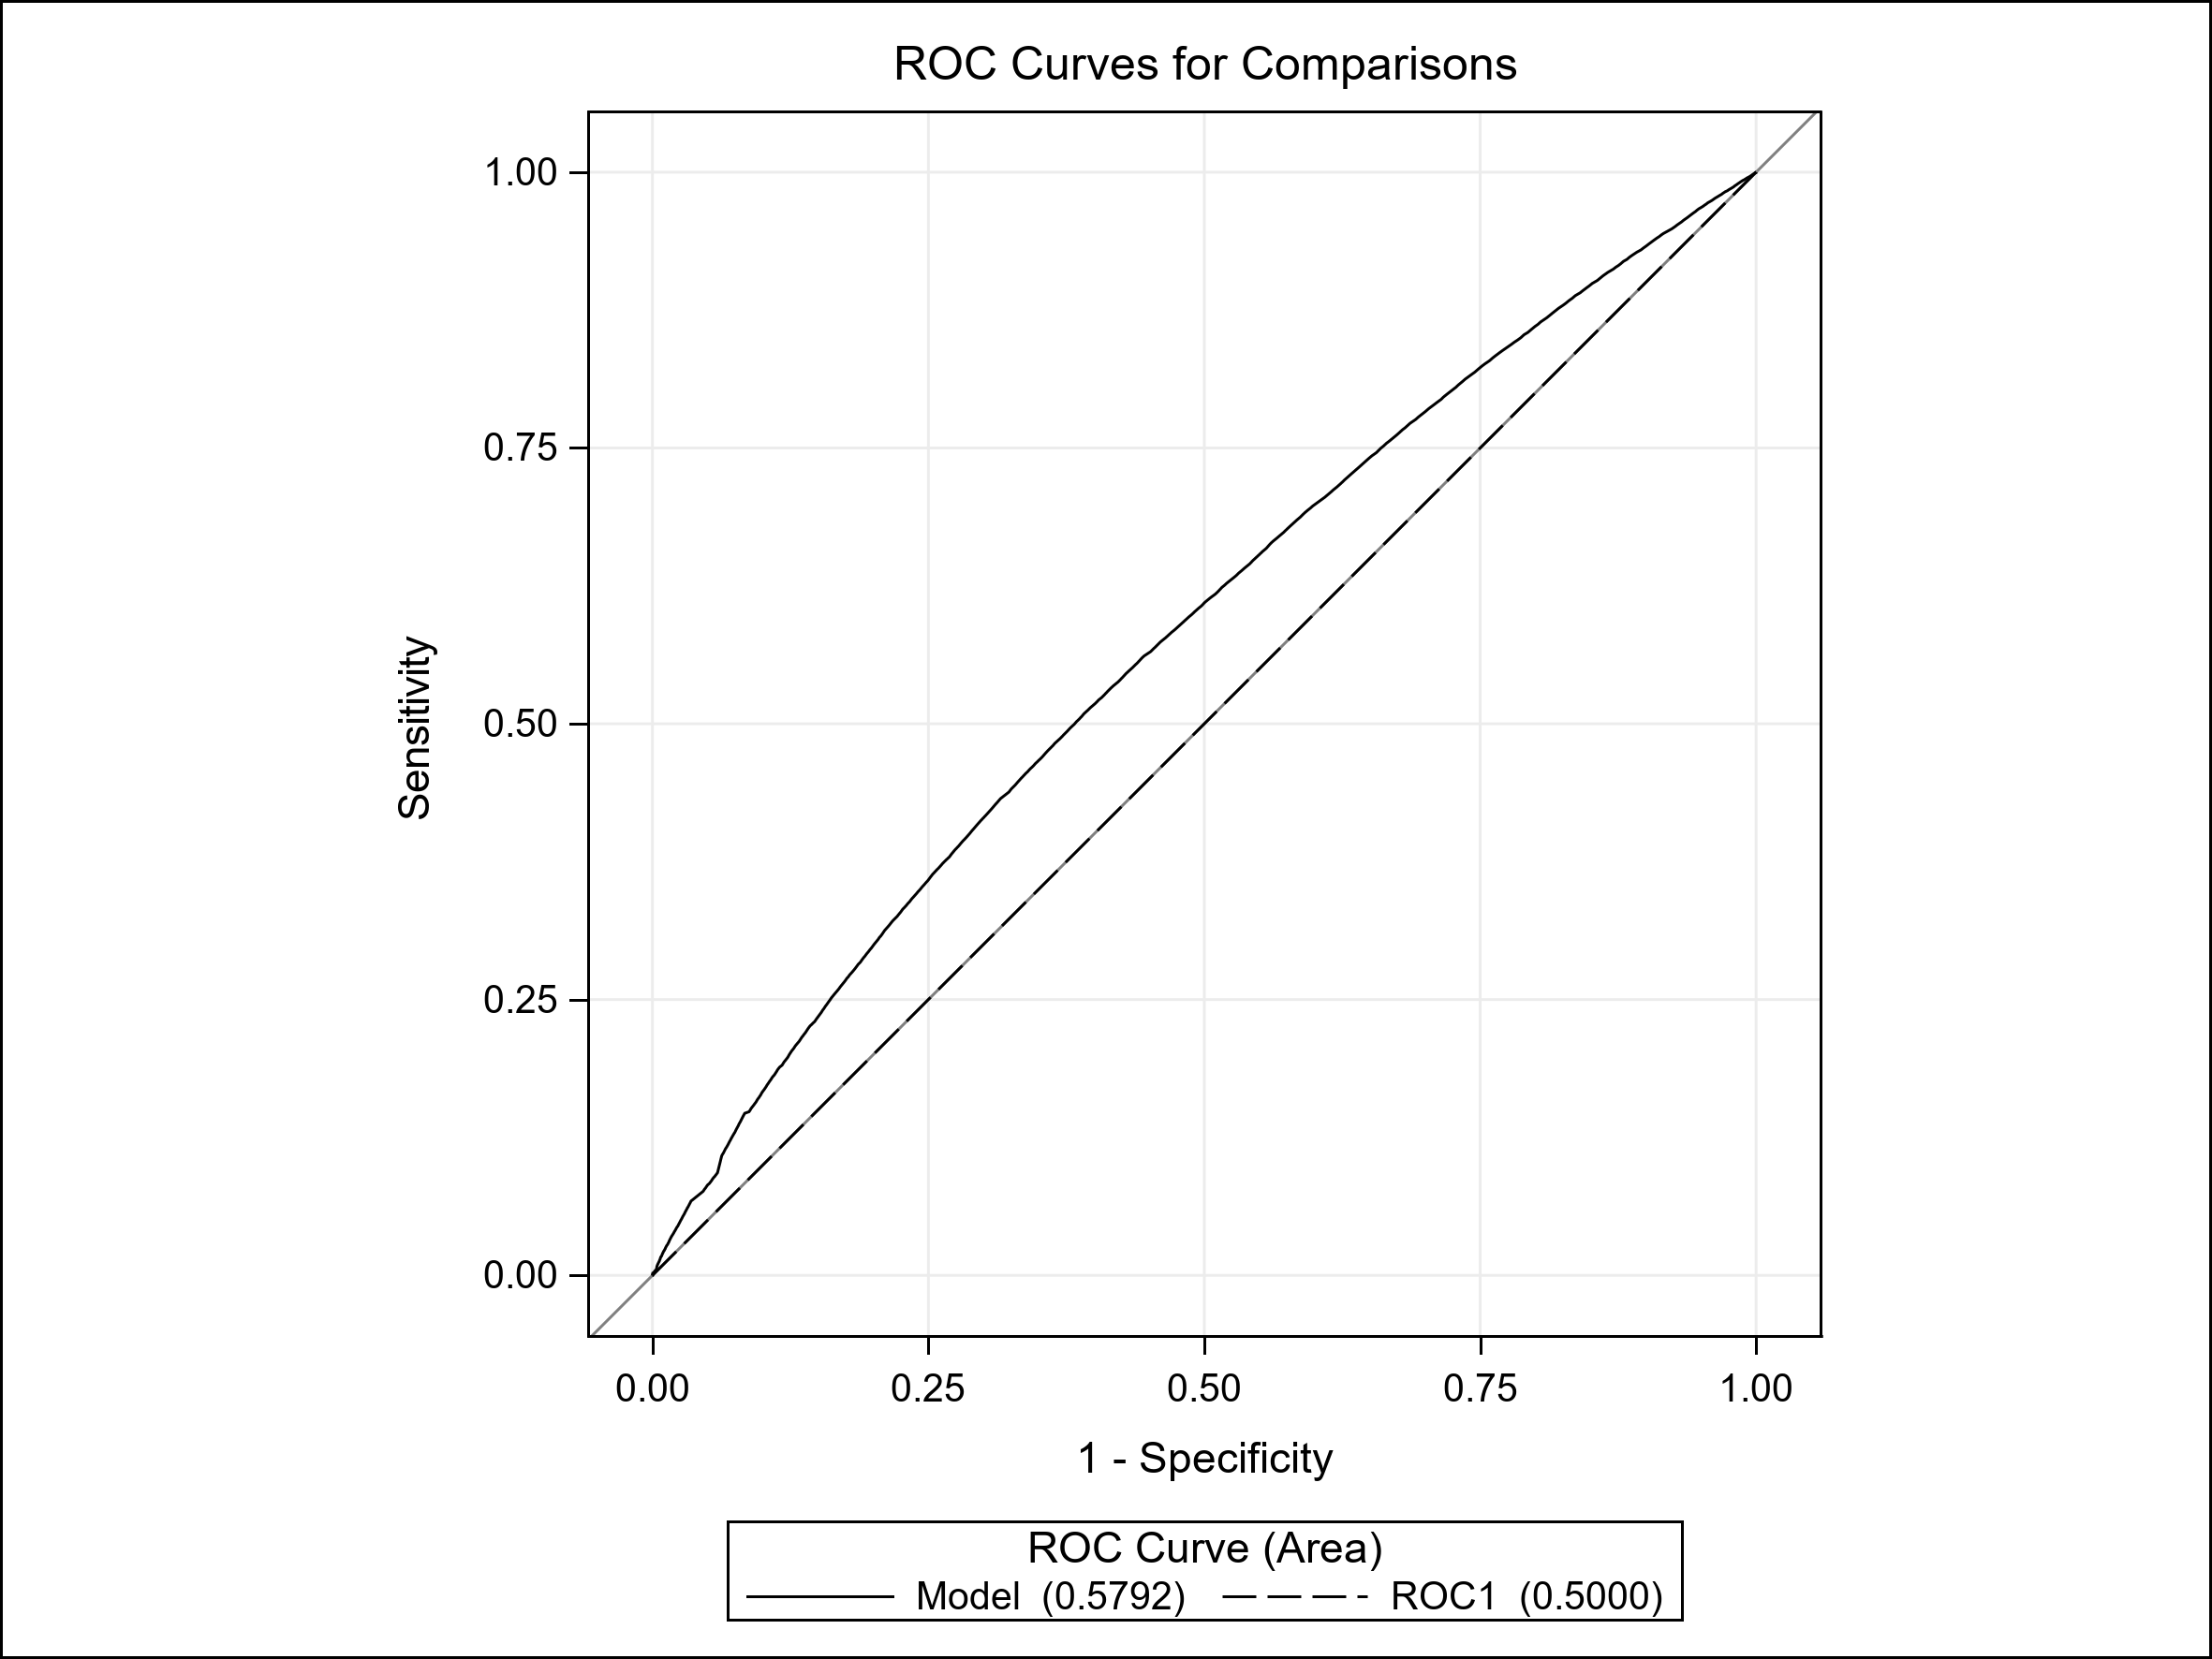
\includegraphics[width=0.9\textwidth]{./plot/ROC/Main/NUM_orig_upb_ROC_ALL5.png}
\end{minipage}
    \caption{ROC-curve of Credit Score and UPB}
\end{figure}

\begin{figure}[H]
\begin{minipage}{.5\textwidth}
	\centering
	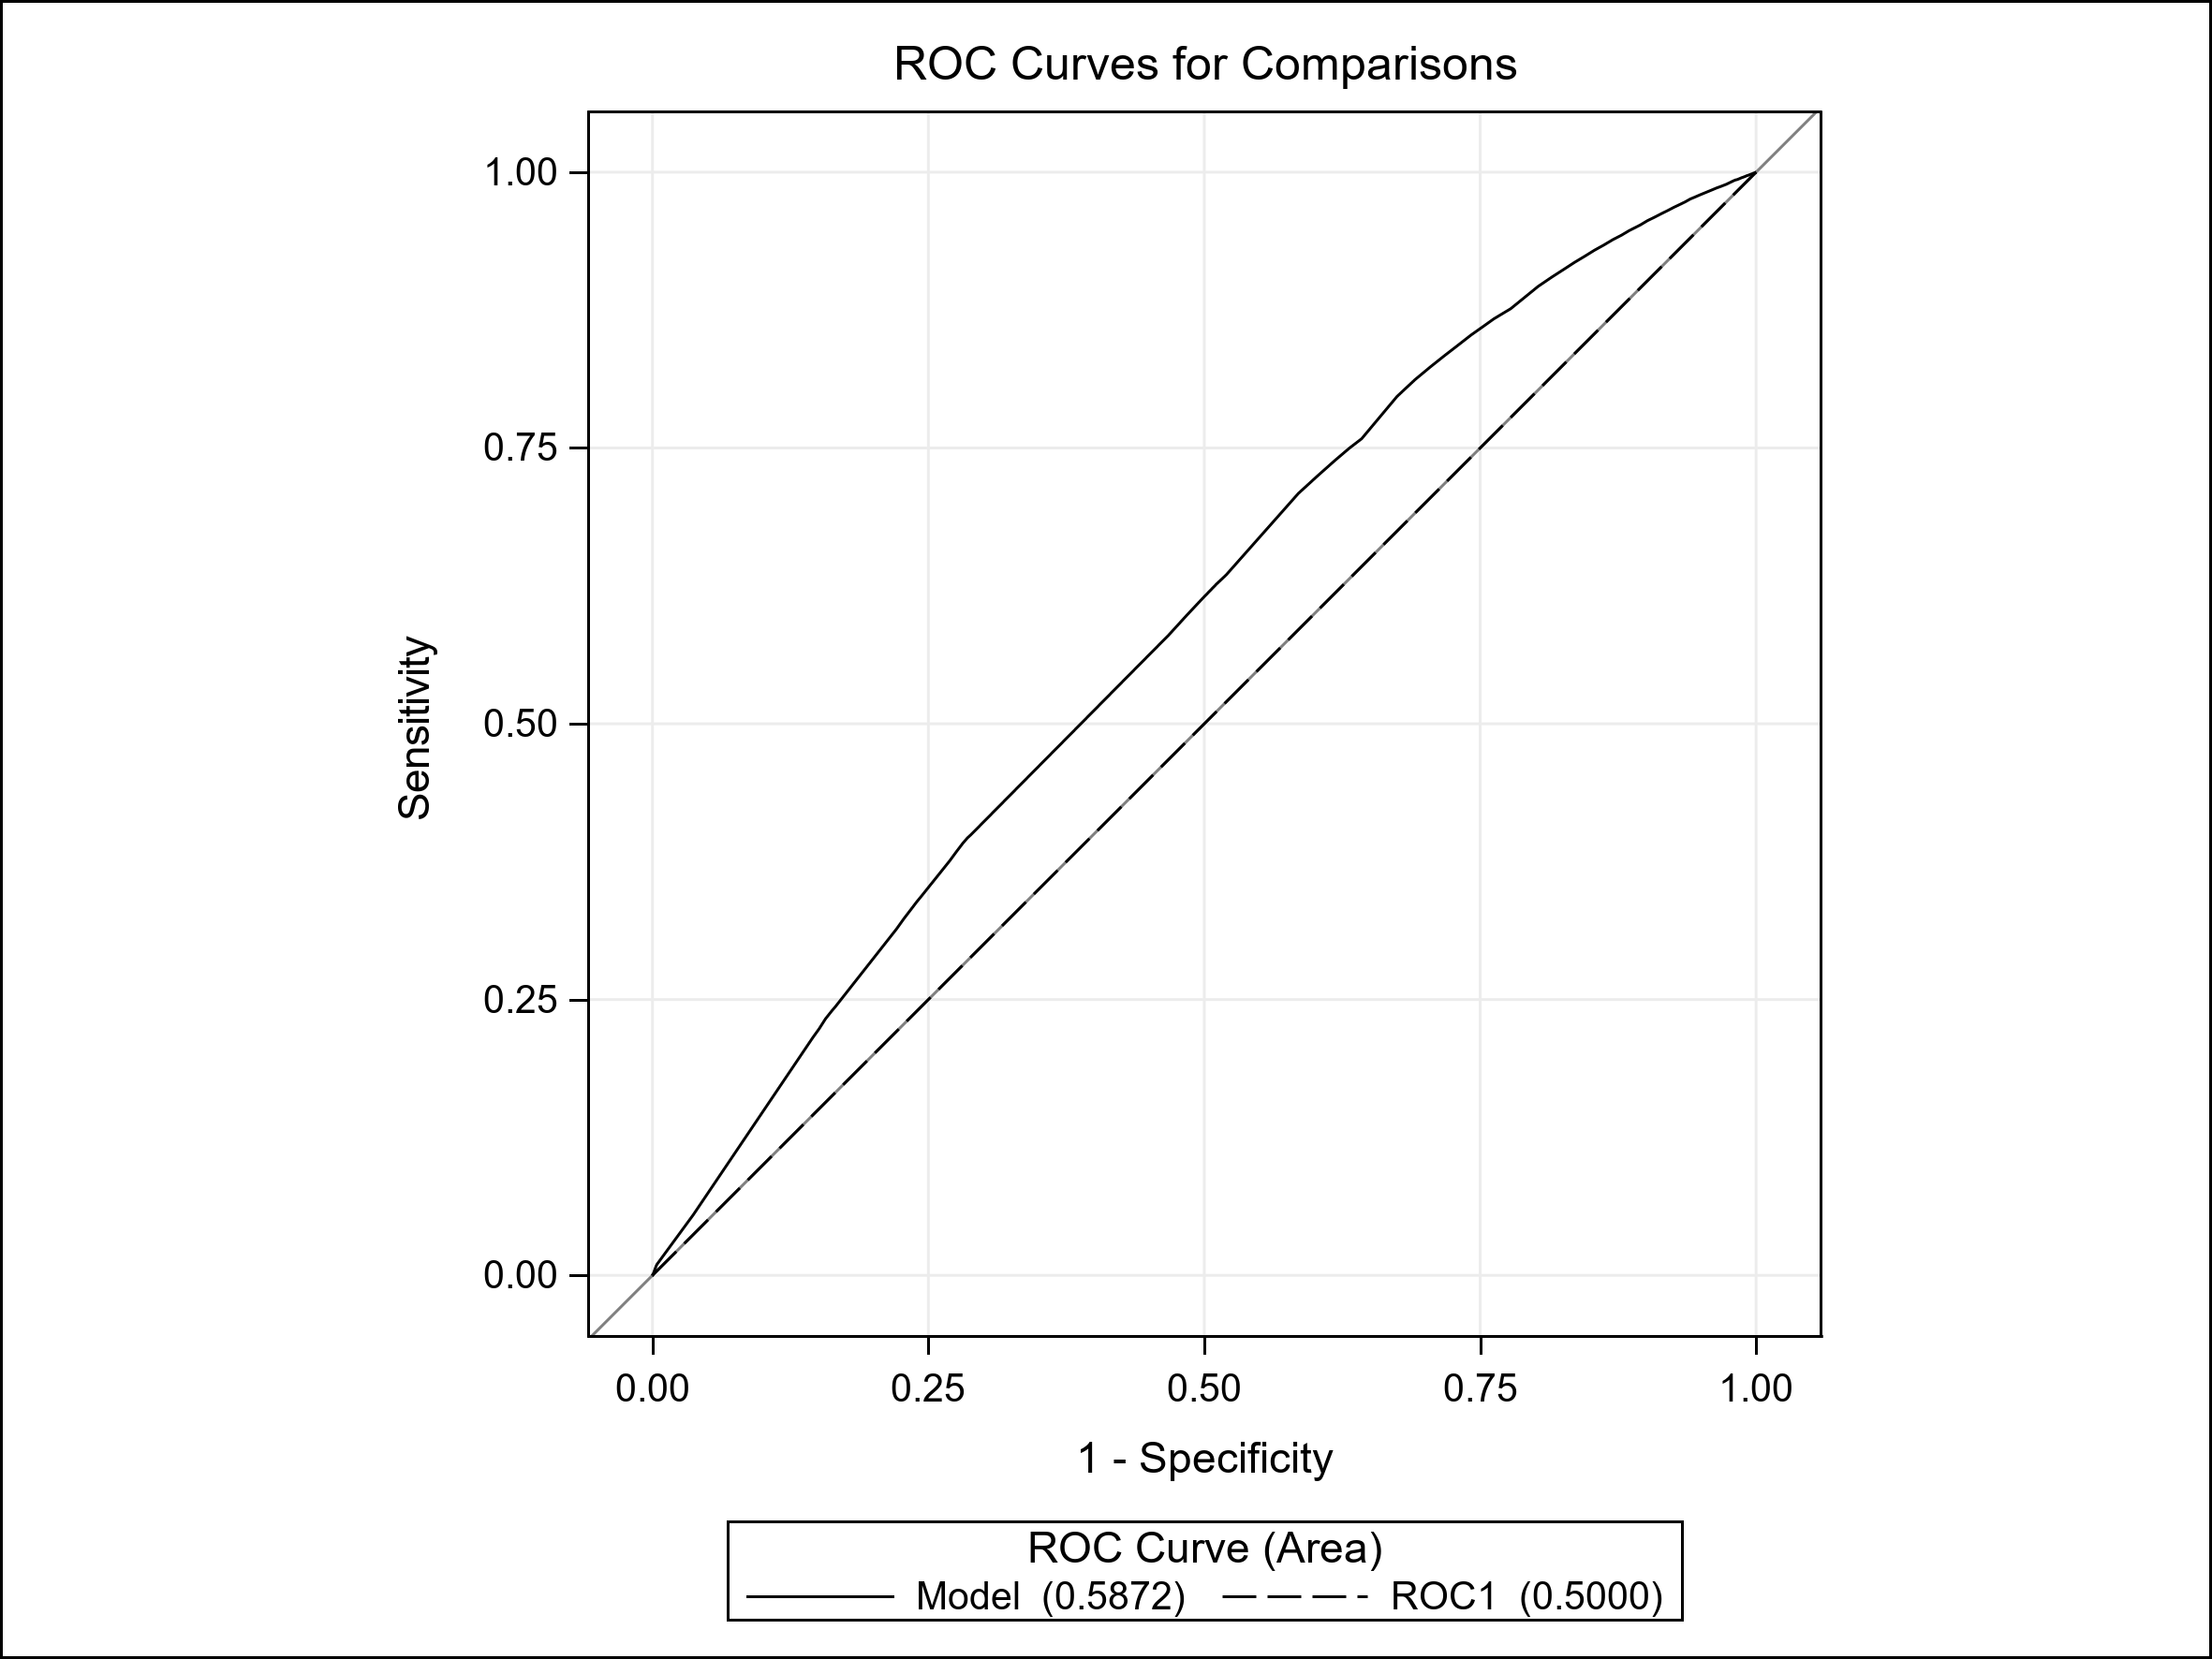
\includegraphics[width=0.9\textwidth]{./plot/ROC/Main/NUM_cltv_ROC_ALL5.png}
\end{minipage}%
\begin{minipage}{.5\textwidth}
	\centering
	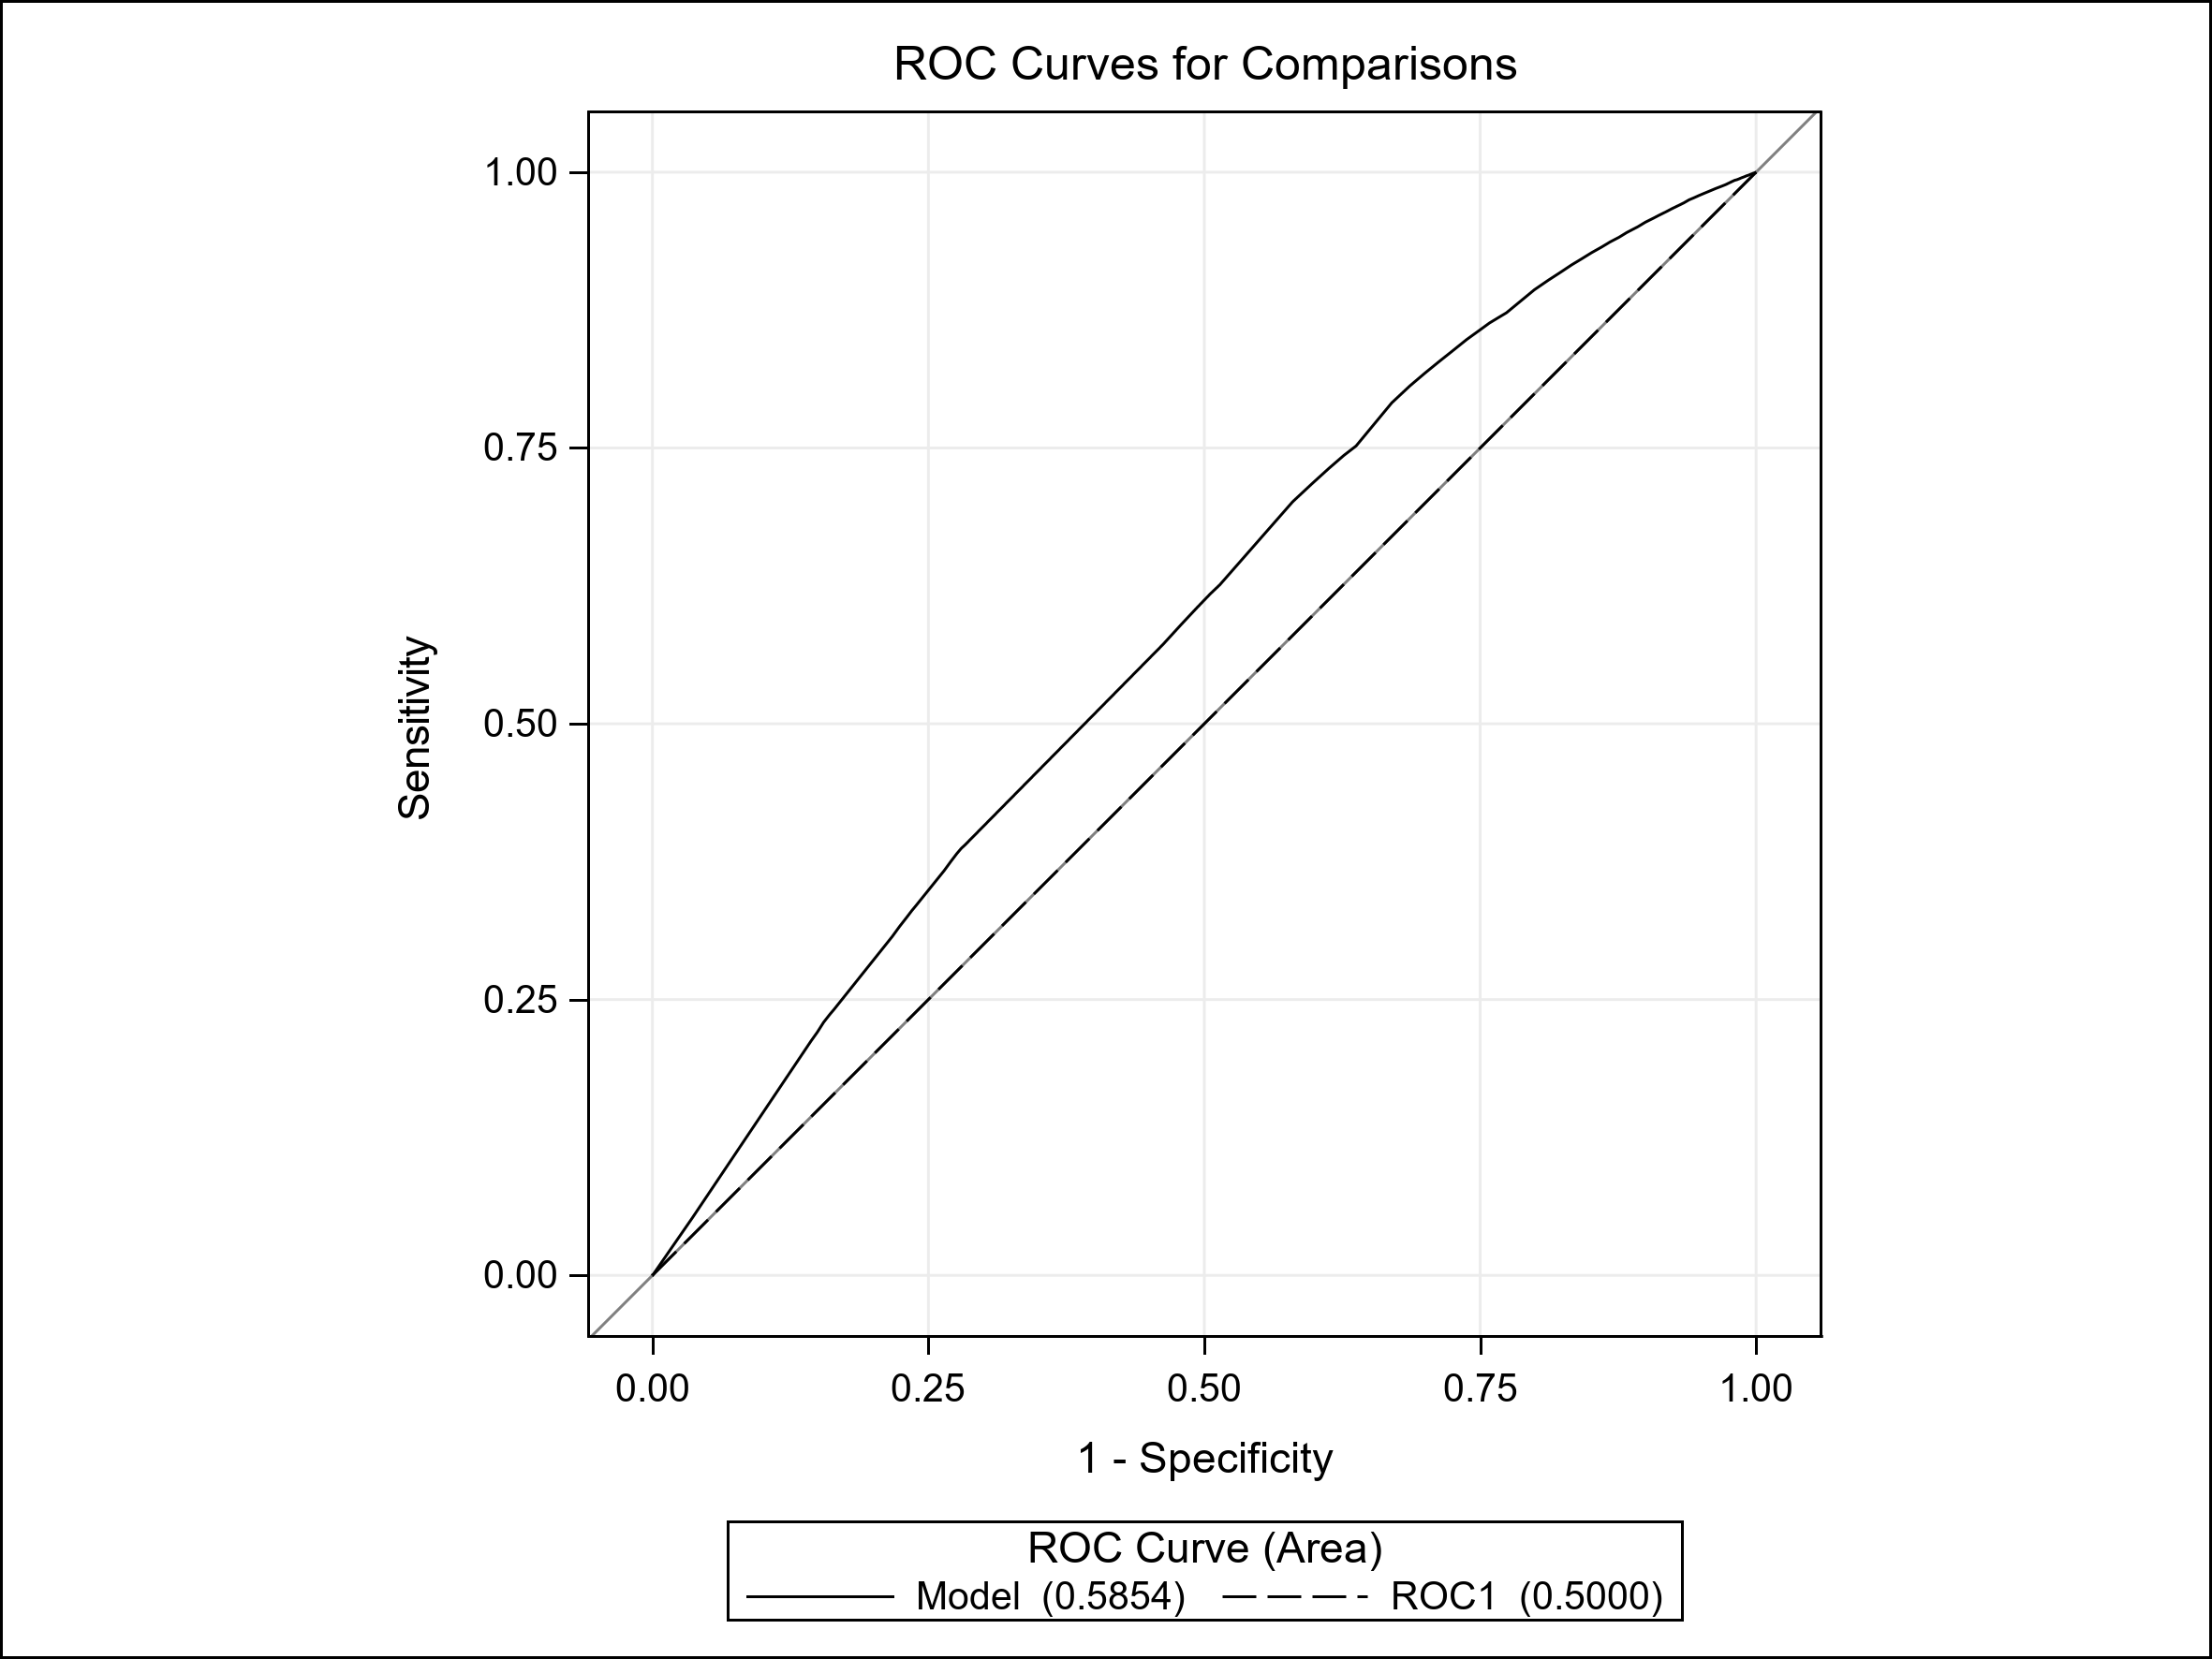
\includegraphics[width=0.9\textwidth]{./plot/ROC/NUM_ltv_ROC_ALL5.png}
\end{minipage}
    \caption{ROC-curve of CLTV and LTV}
\end{figure}

\begin{figure}[H]
\begin{minipage}{.5\textwidth}
	\centering
	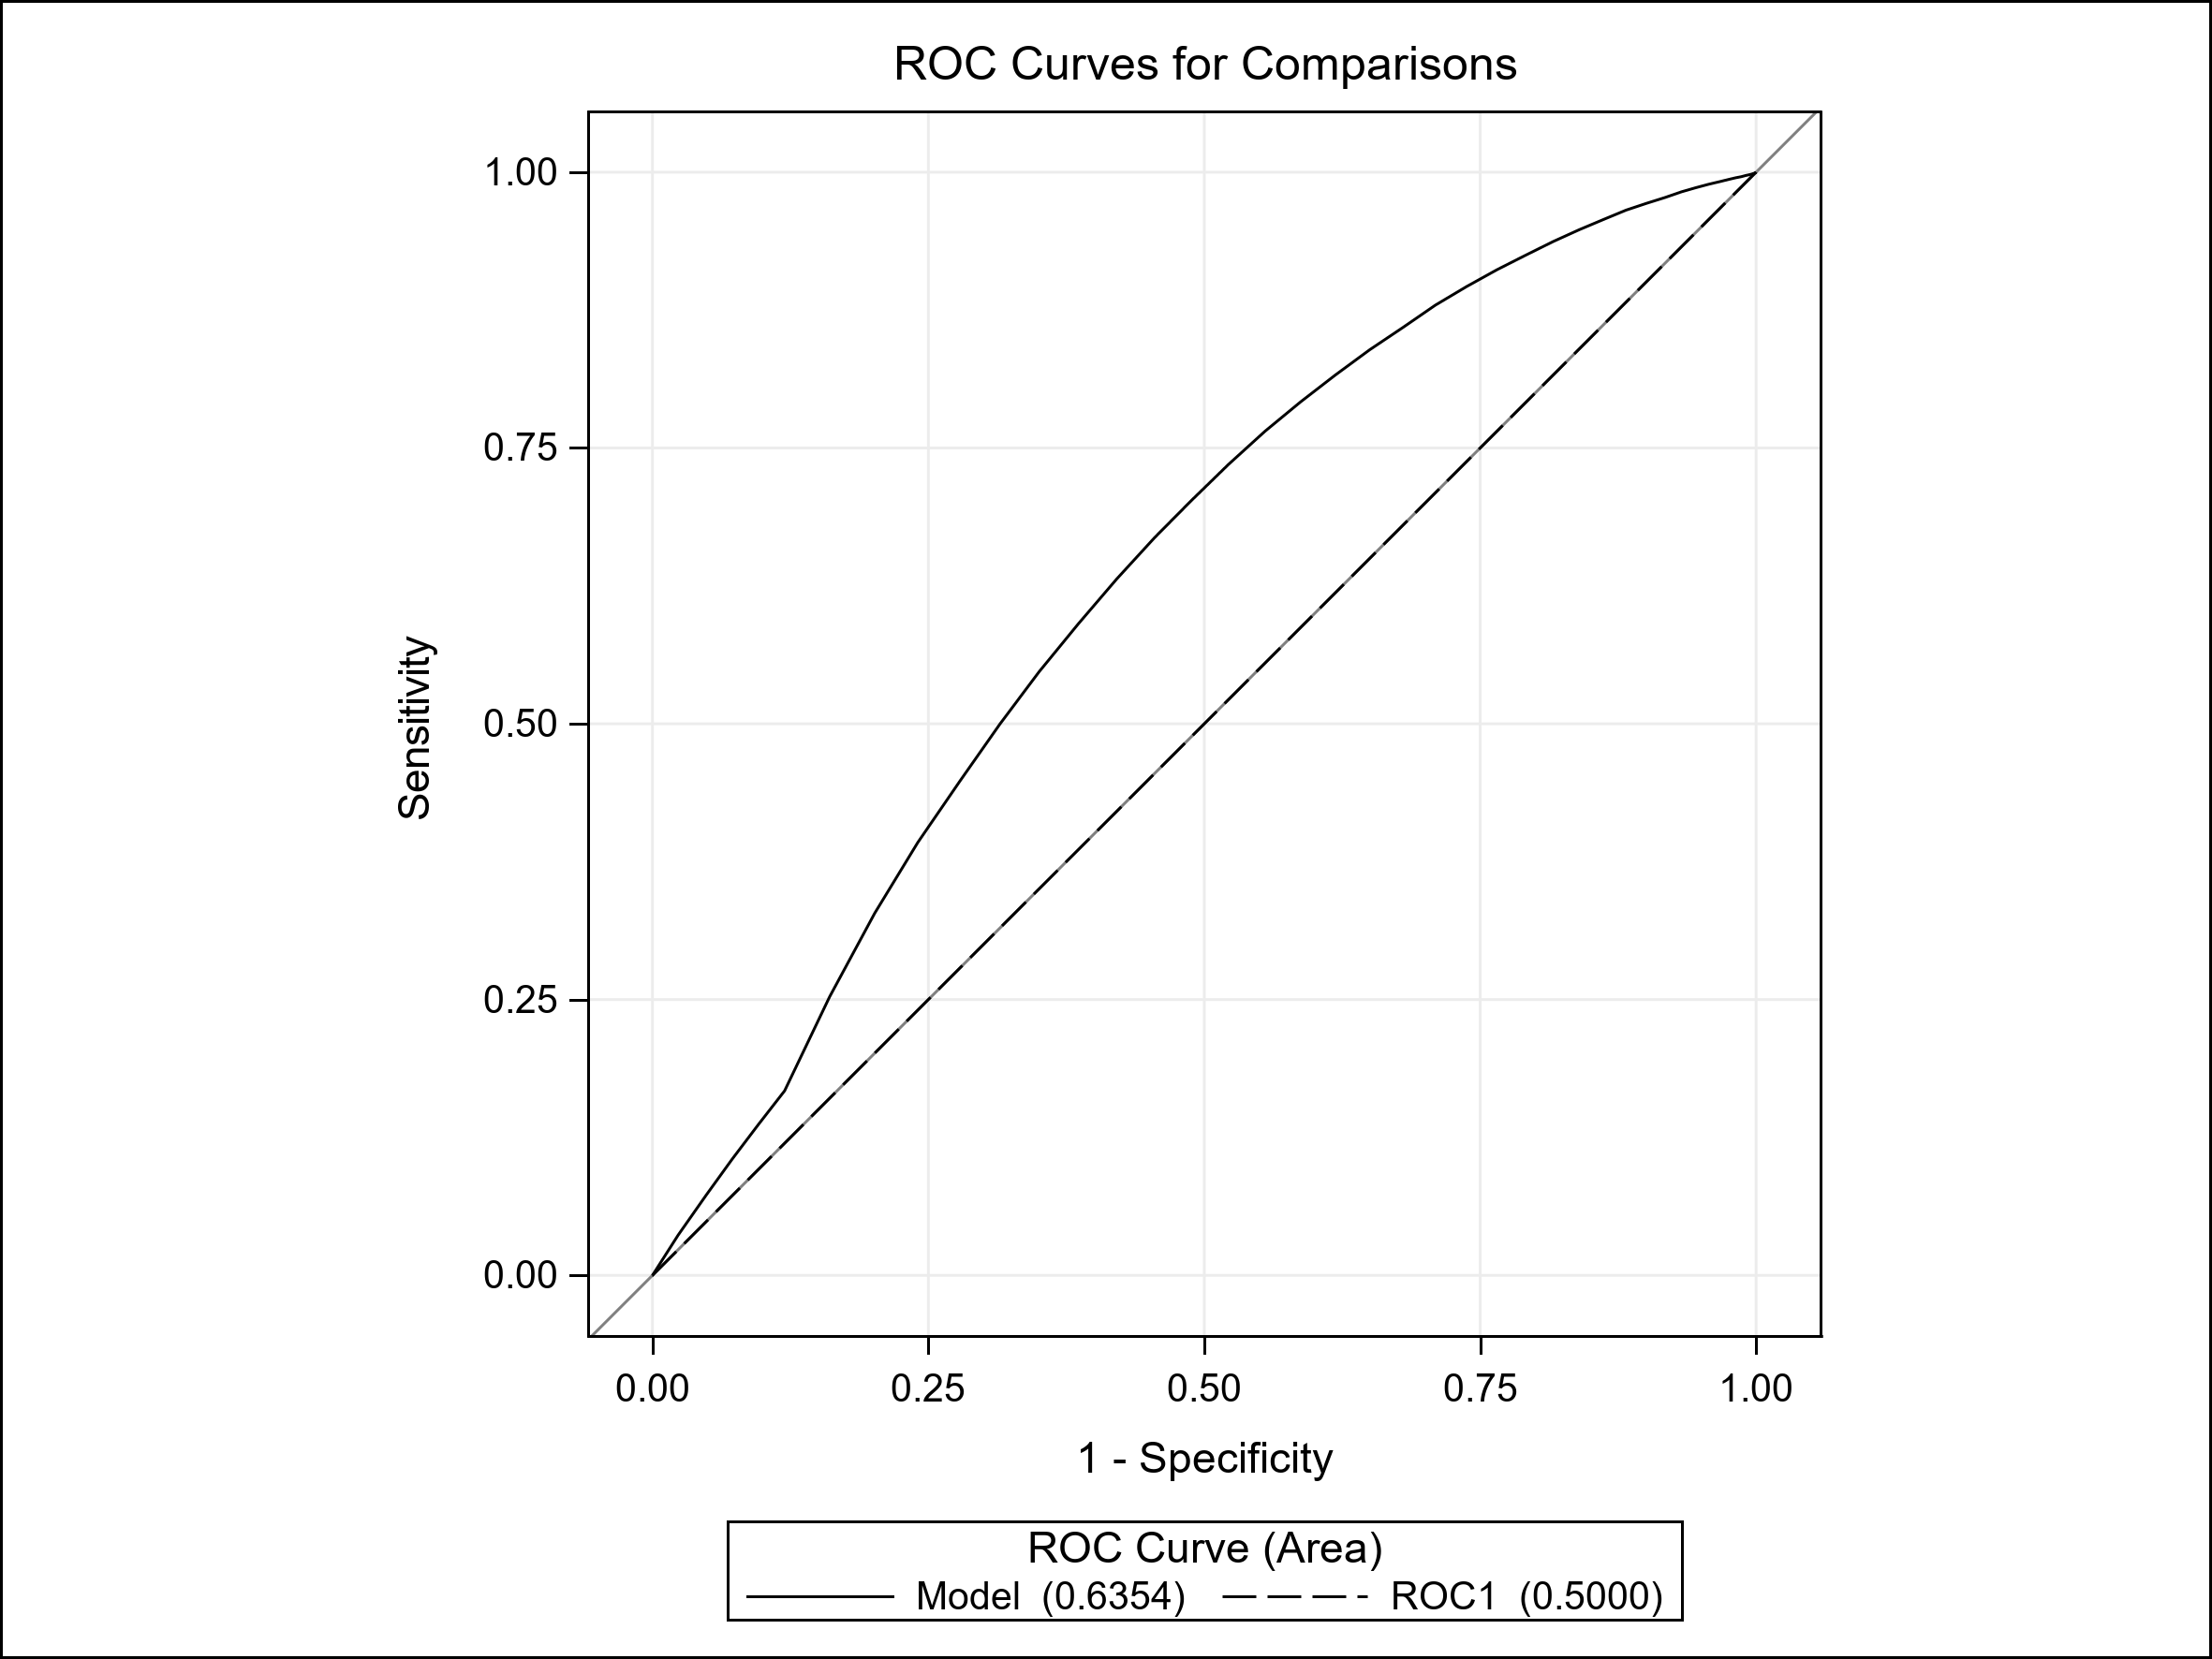
\includegraphics[width=0.9\textwidth]{./plot/ROC/Main/NUM_dti_ROC_ALL5.png}
\end{minipage}%
\begin{minipage}{.5\textwidth}
	\centering
	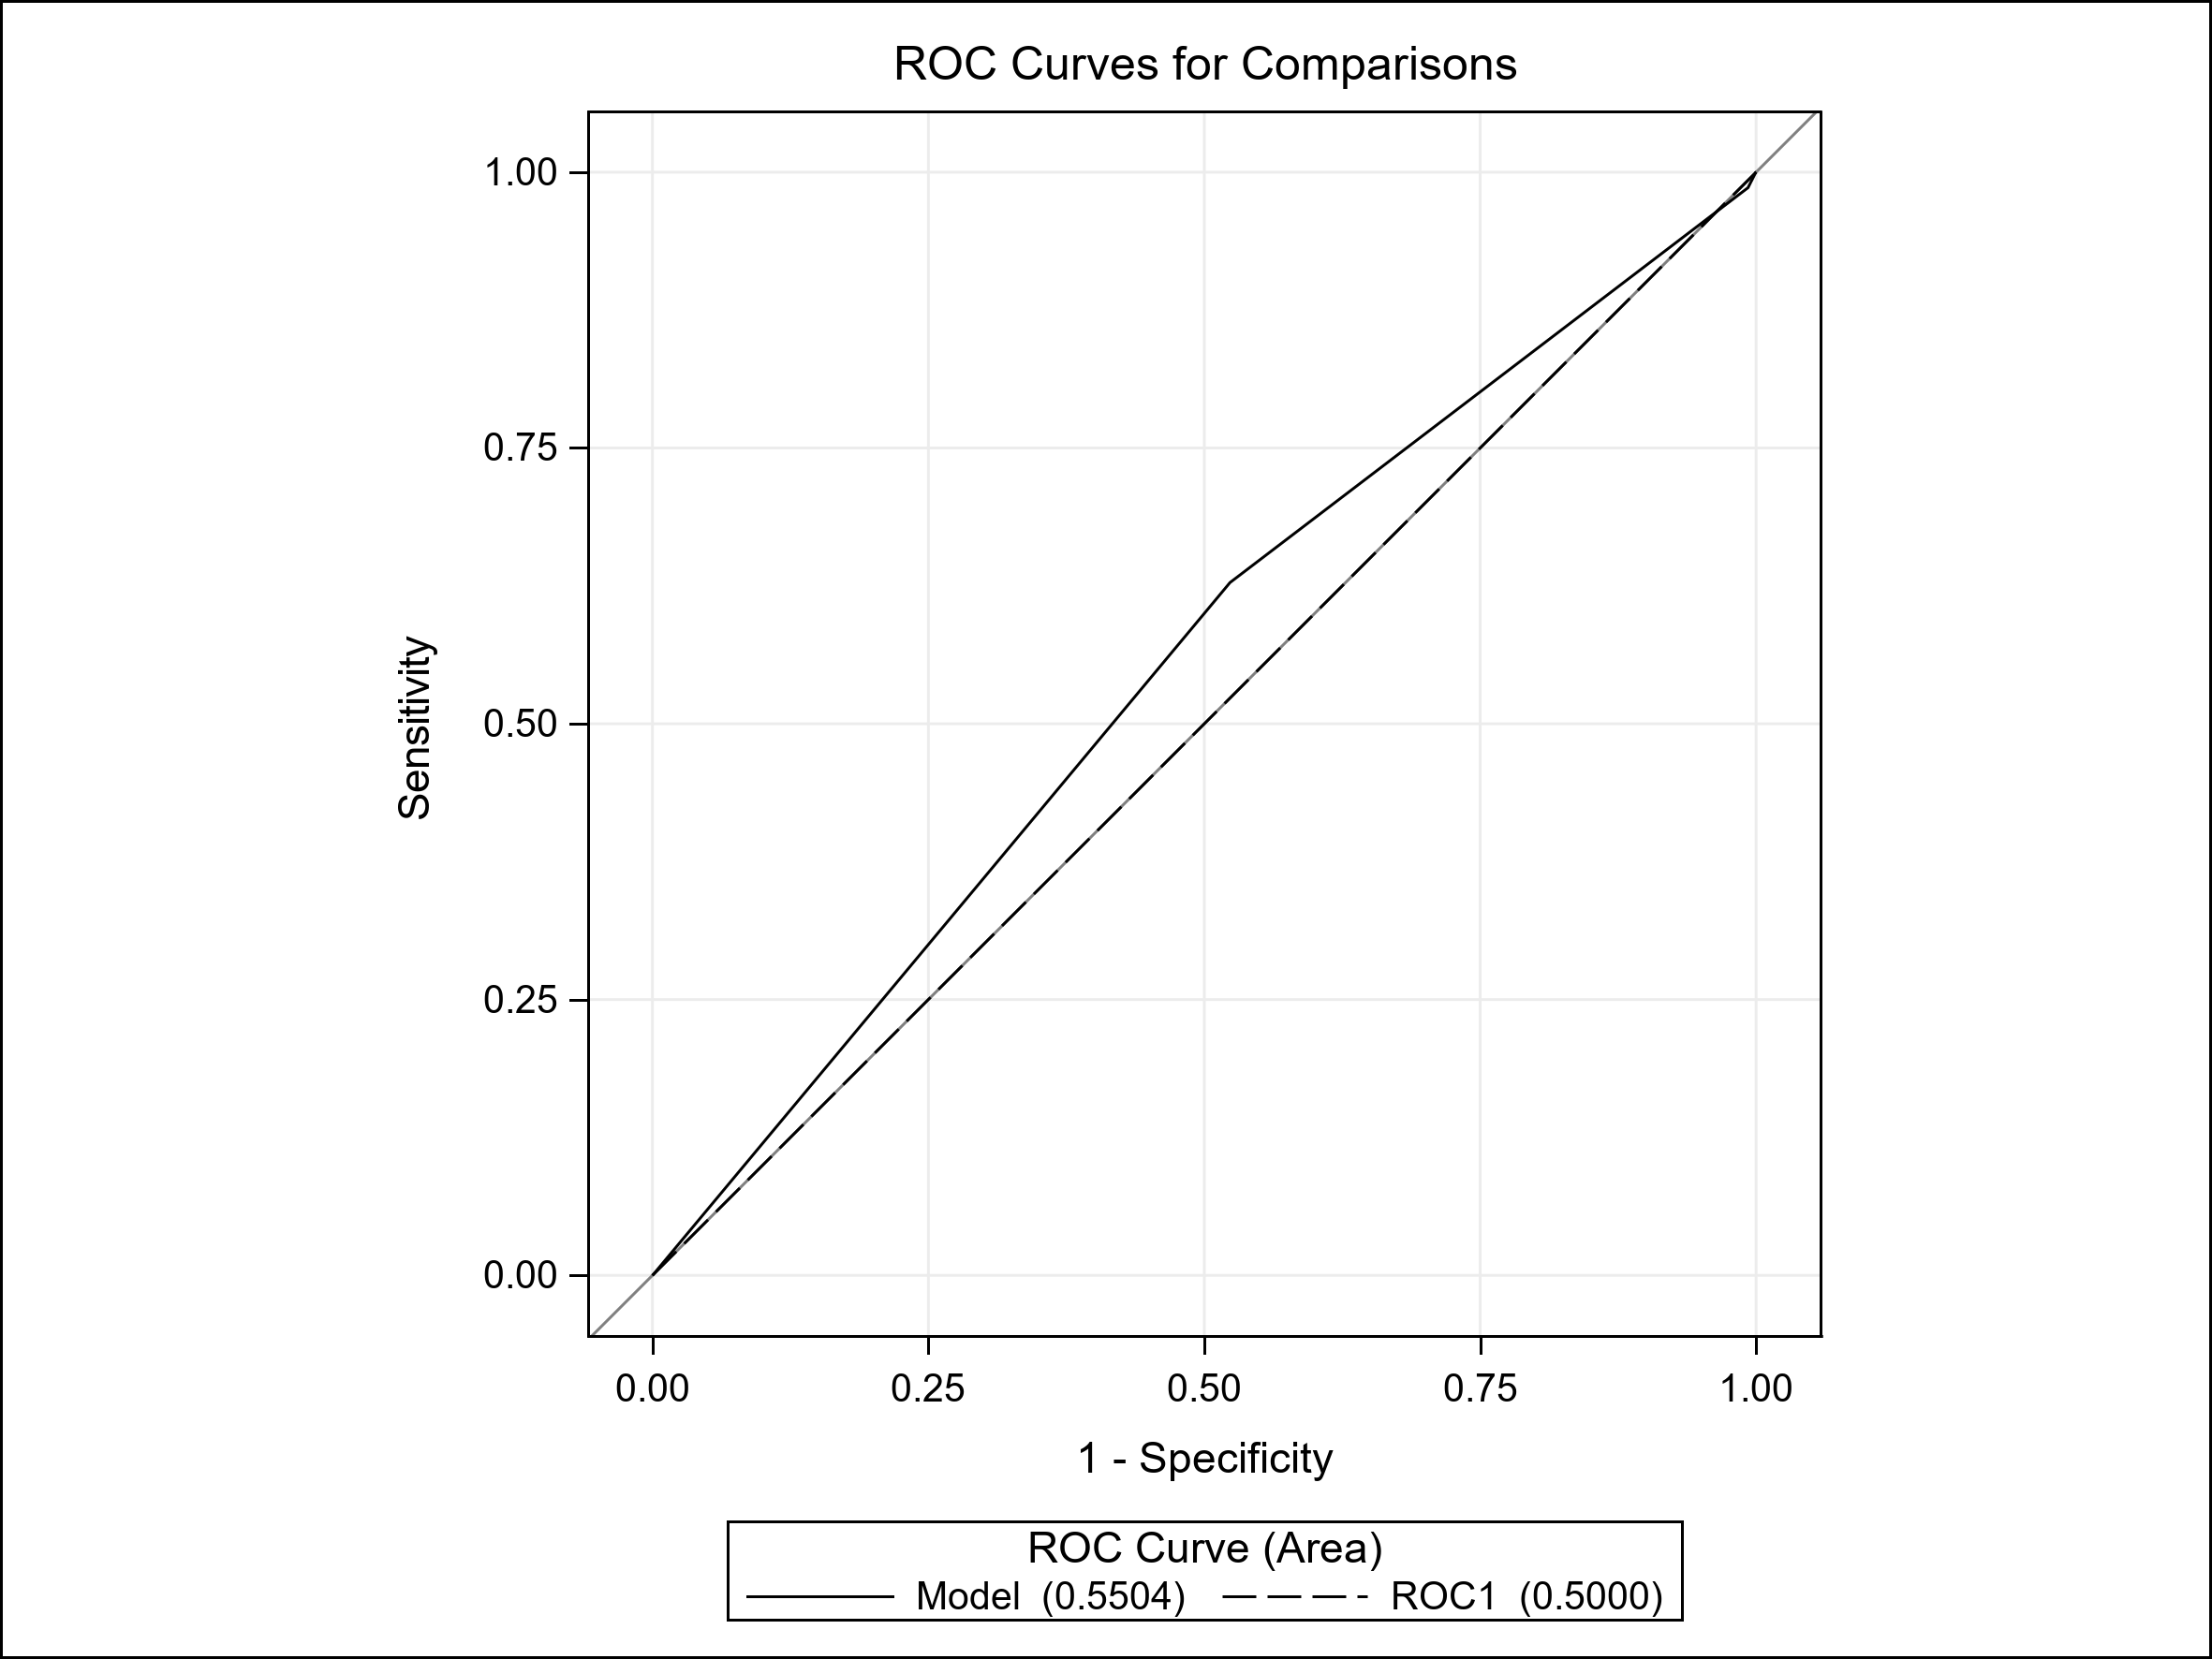
\includegraphics[width=0.9\textwidth]{./plot/ROC/Main/NUM_cnt_borr_ROC_ALL5.png}
\end{minipage}
    \caption{ROC-curve of DTI and No Borrowers}
\end{figure}

\begin{figure}[H]
\begin{minipage}{.5\textwidth}
	\centering
	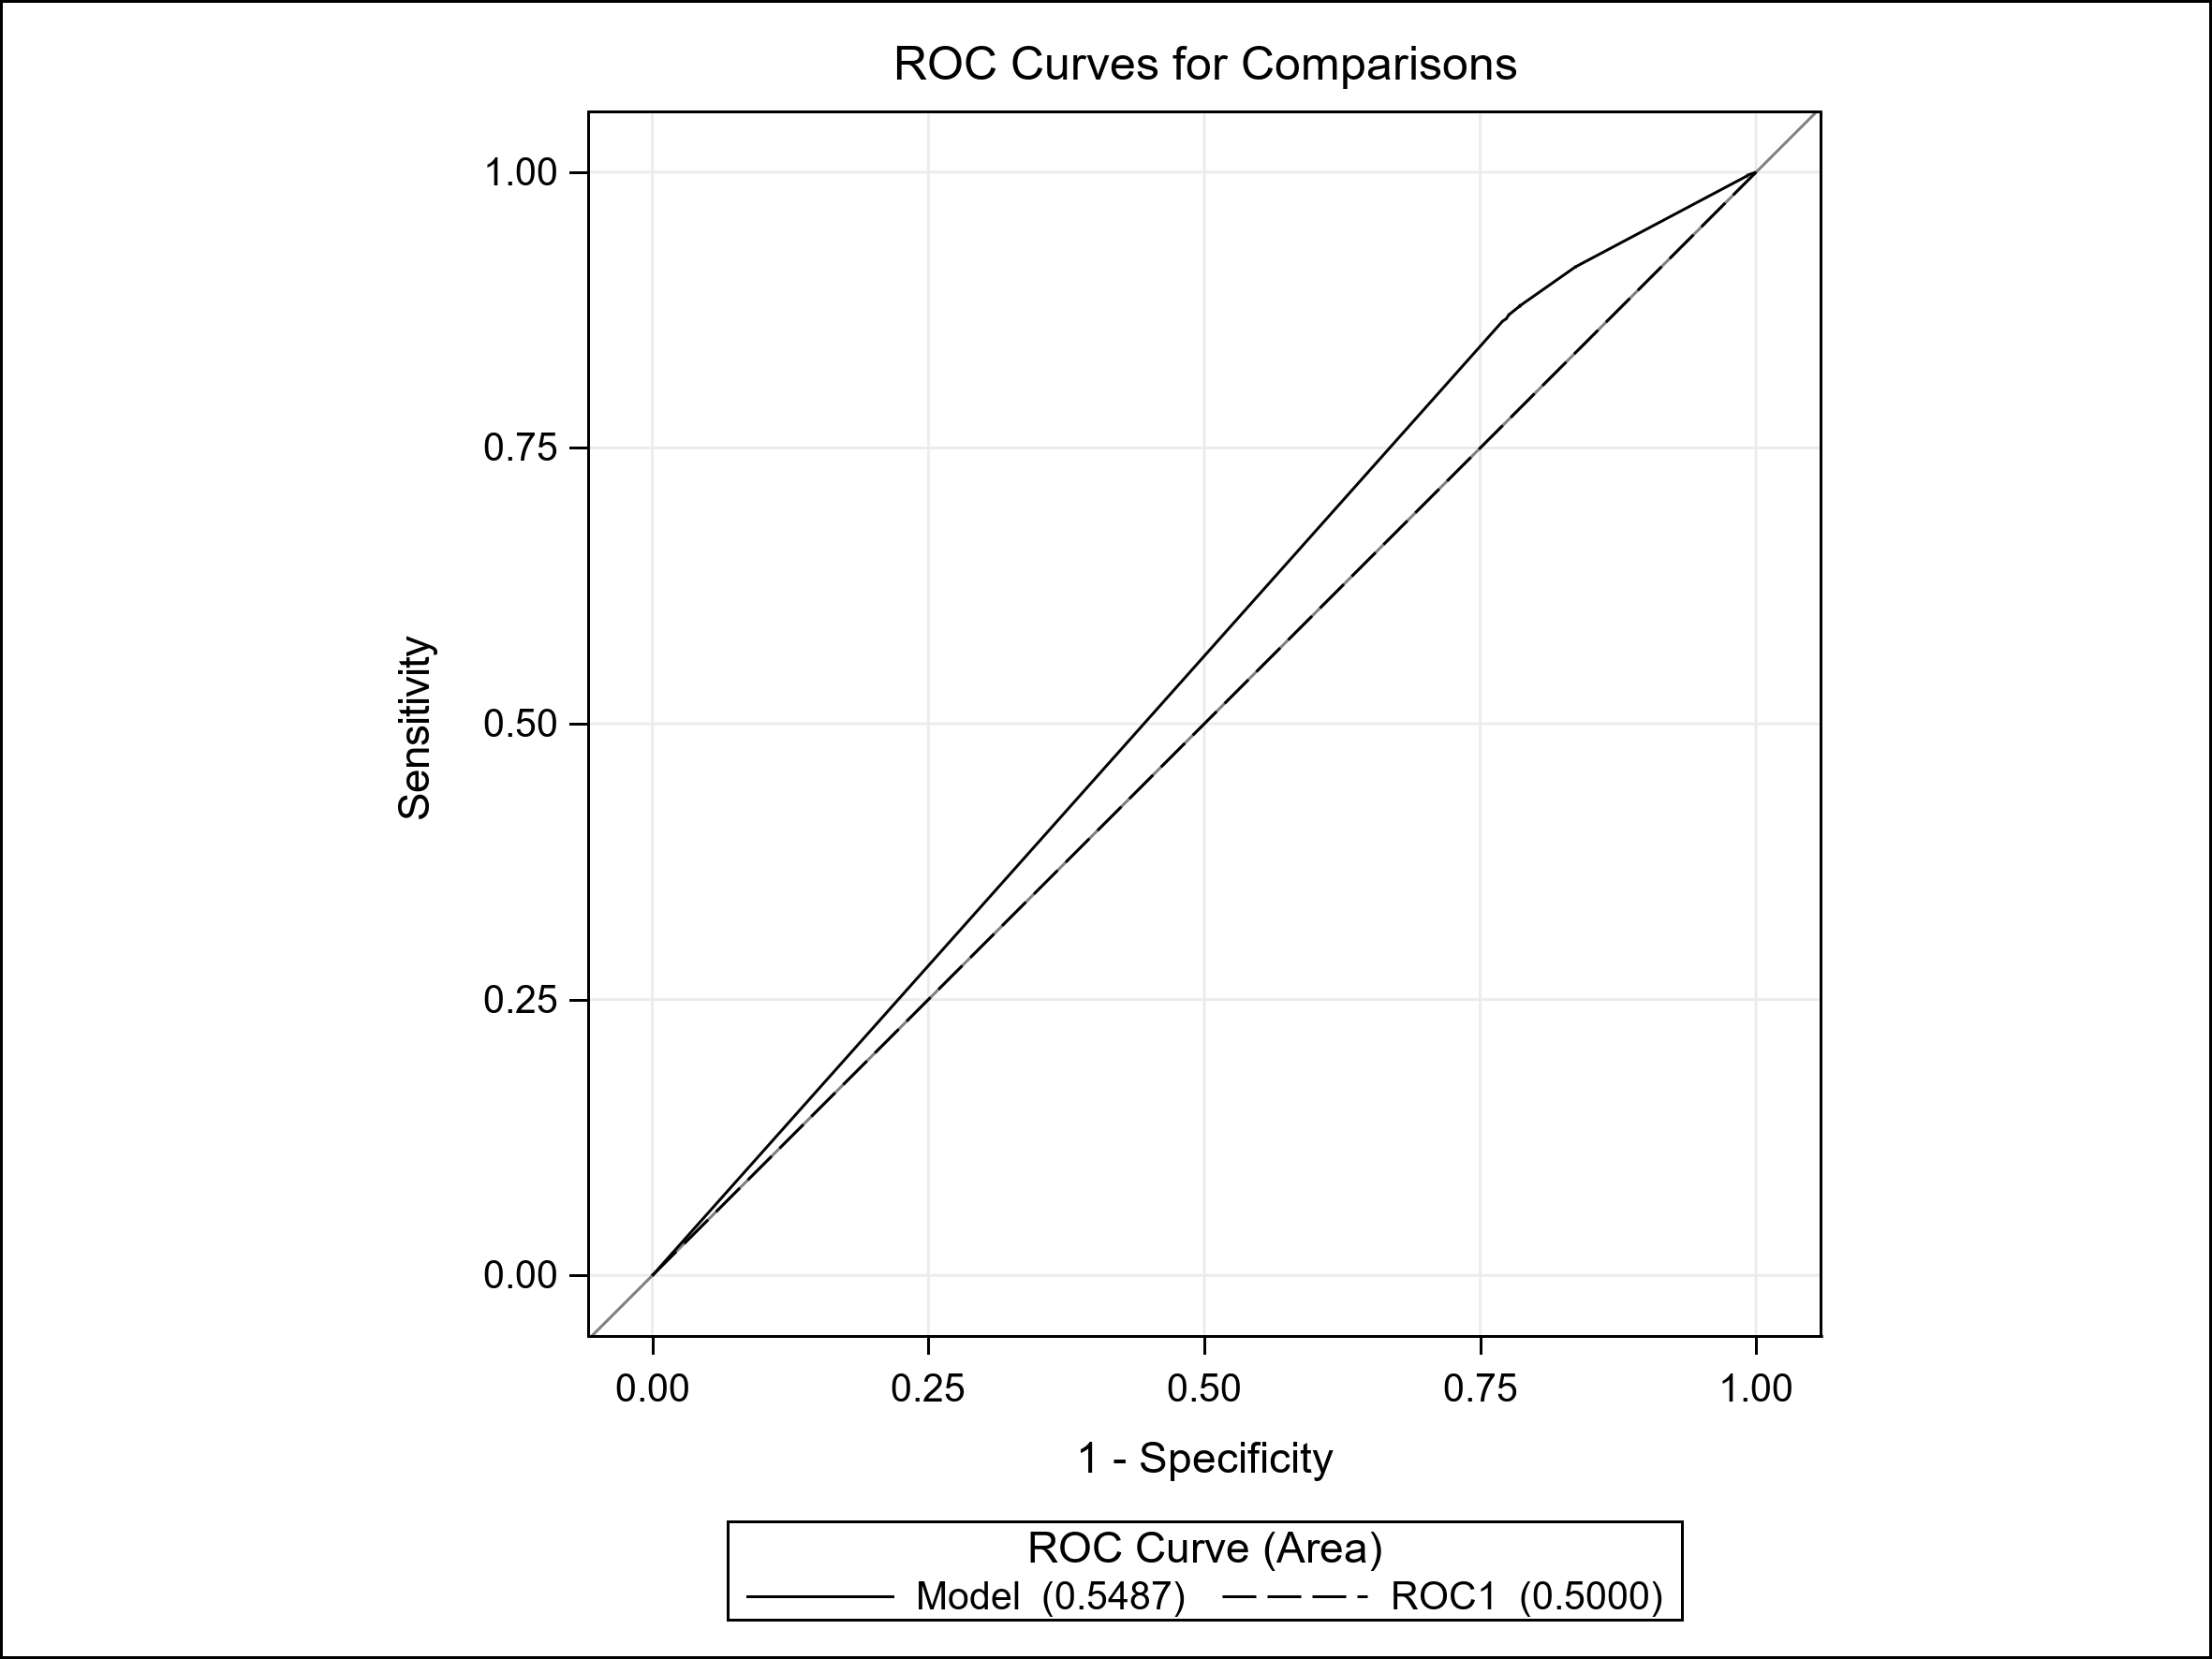
\includegraphics[width=0.9\textwidth]{./plot/ROC/NUM_orig_loan_term_ROC_ALL5.png}
\end{minipage}%
\begin{minipage}{.5\textwidth}
	\centering
	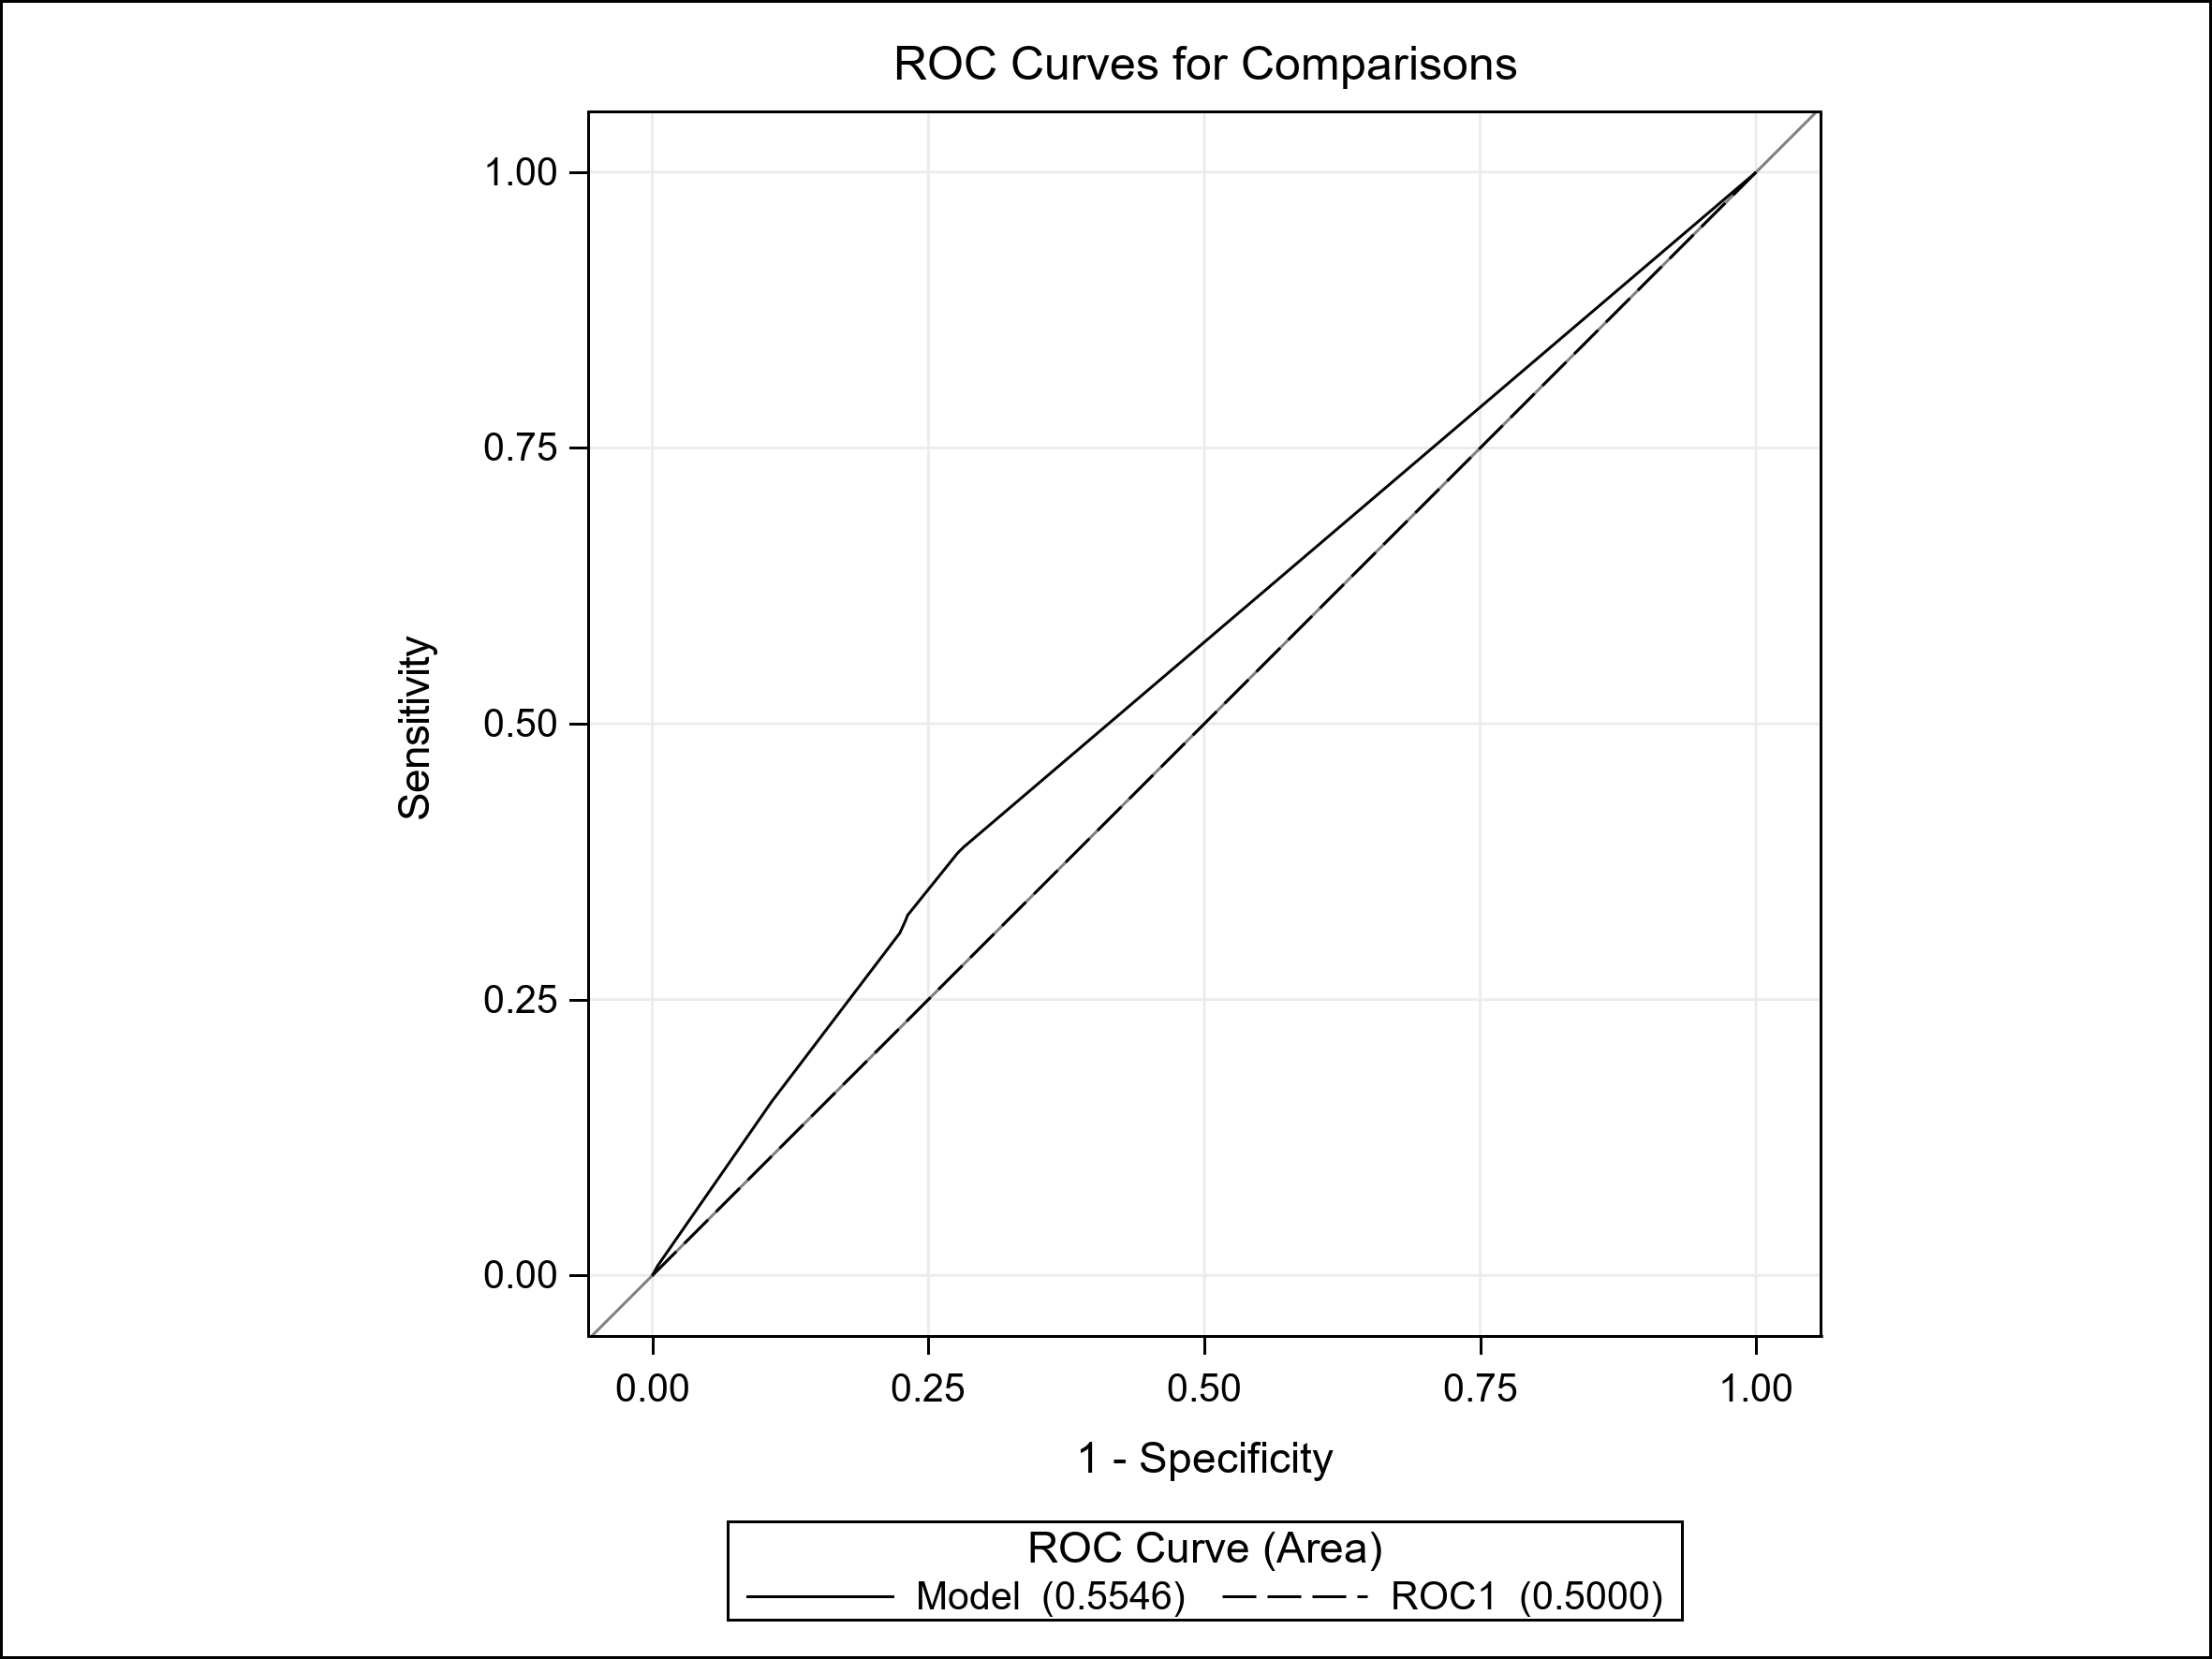
\includegraphics[width=0.9\textwidth]{./plot/ROC/NUM_mi_pct_ROC_ALL5.png}
\end{minipage}
    \caption{ROC-curve of Loan Term and MI Perc}
\end{figure}

\begin{figure}[H]
	\centering
	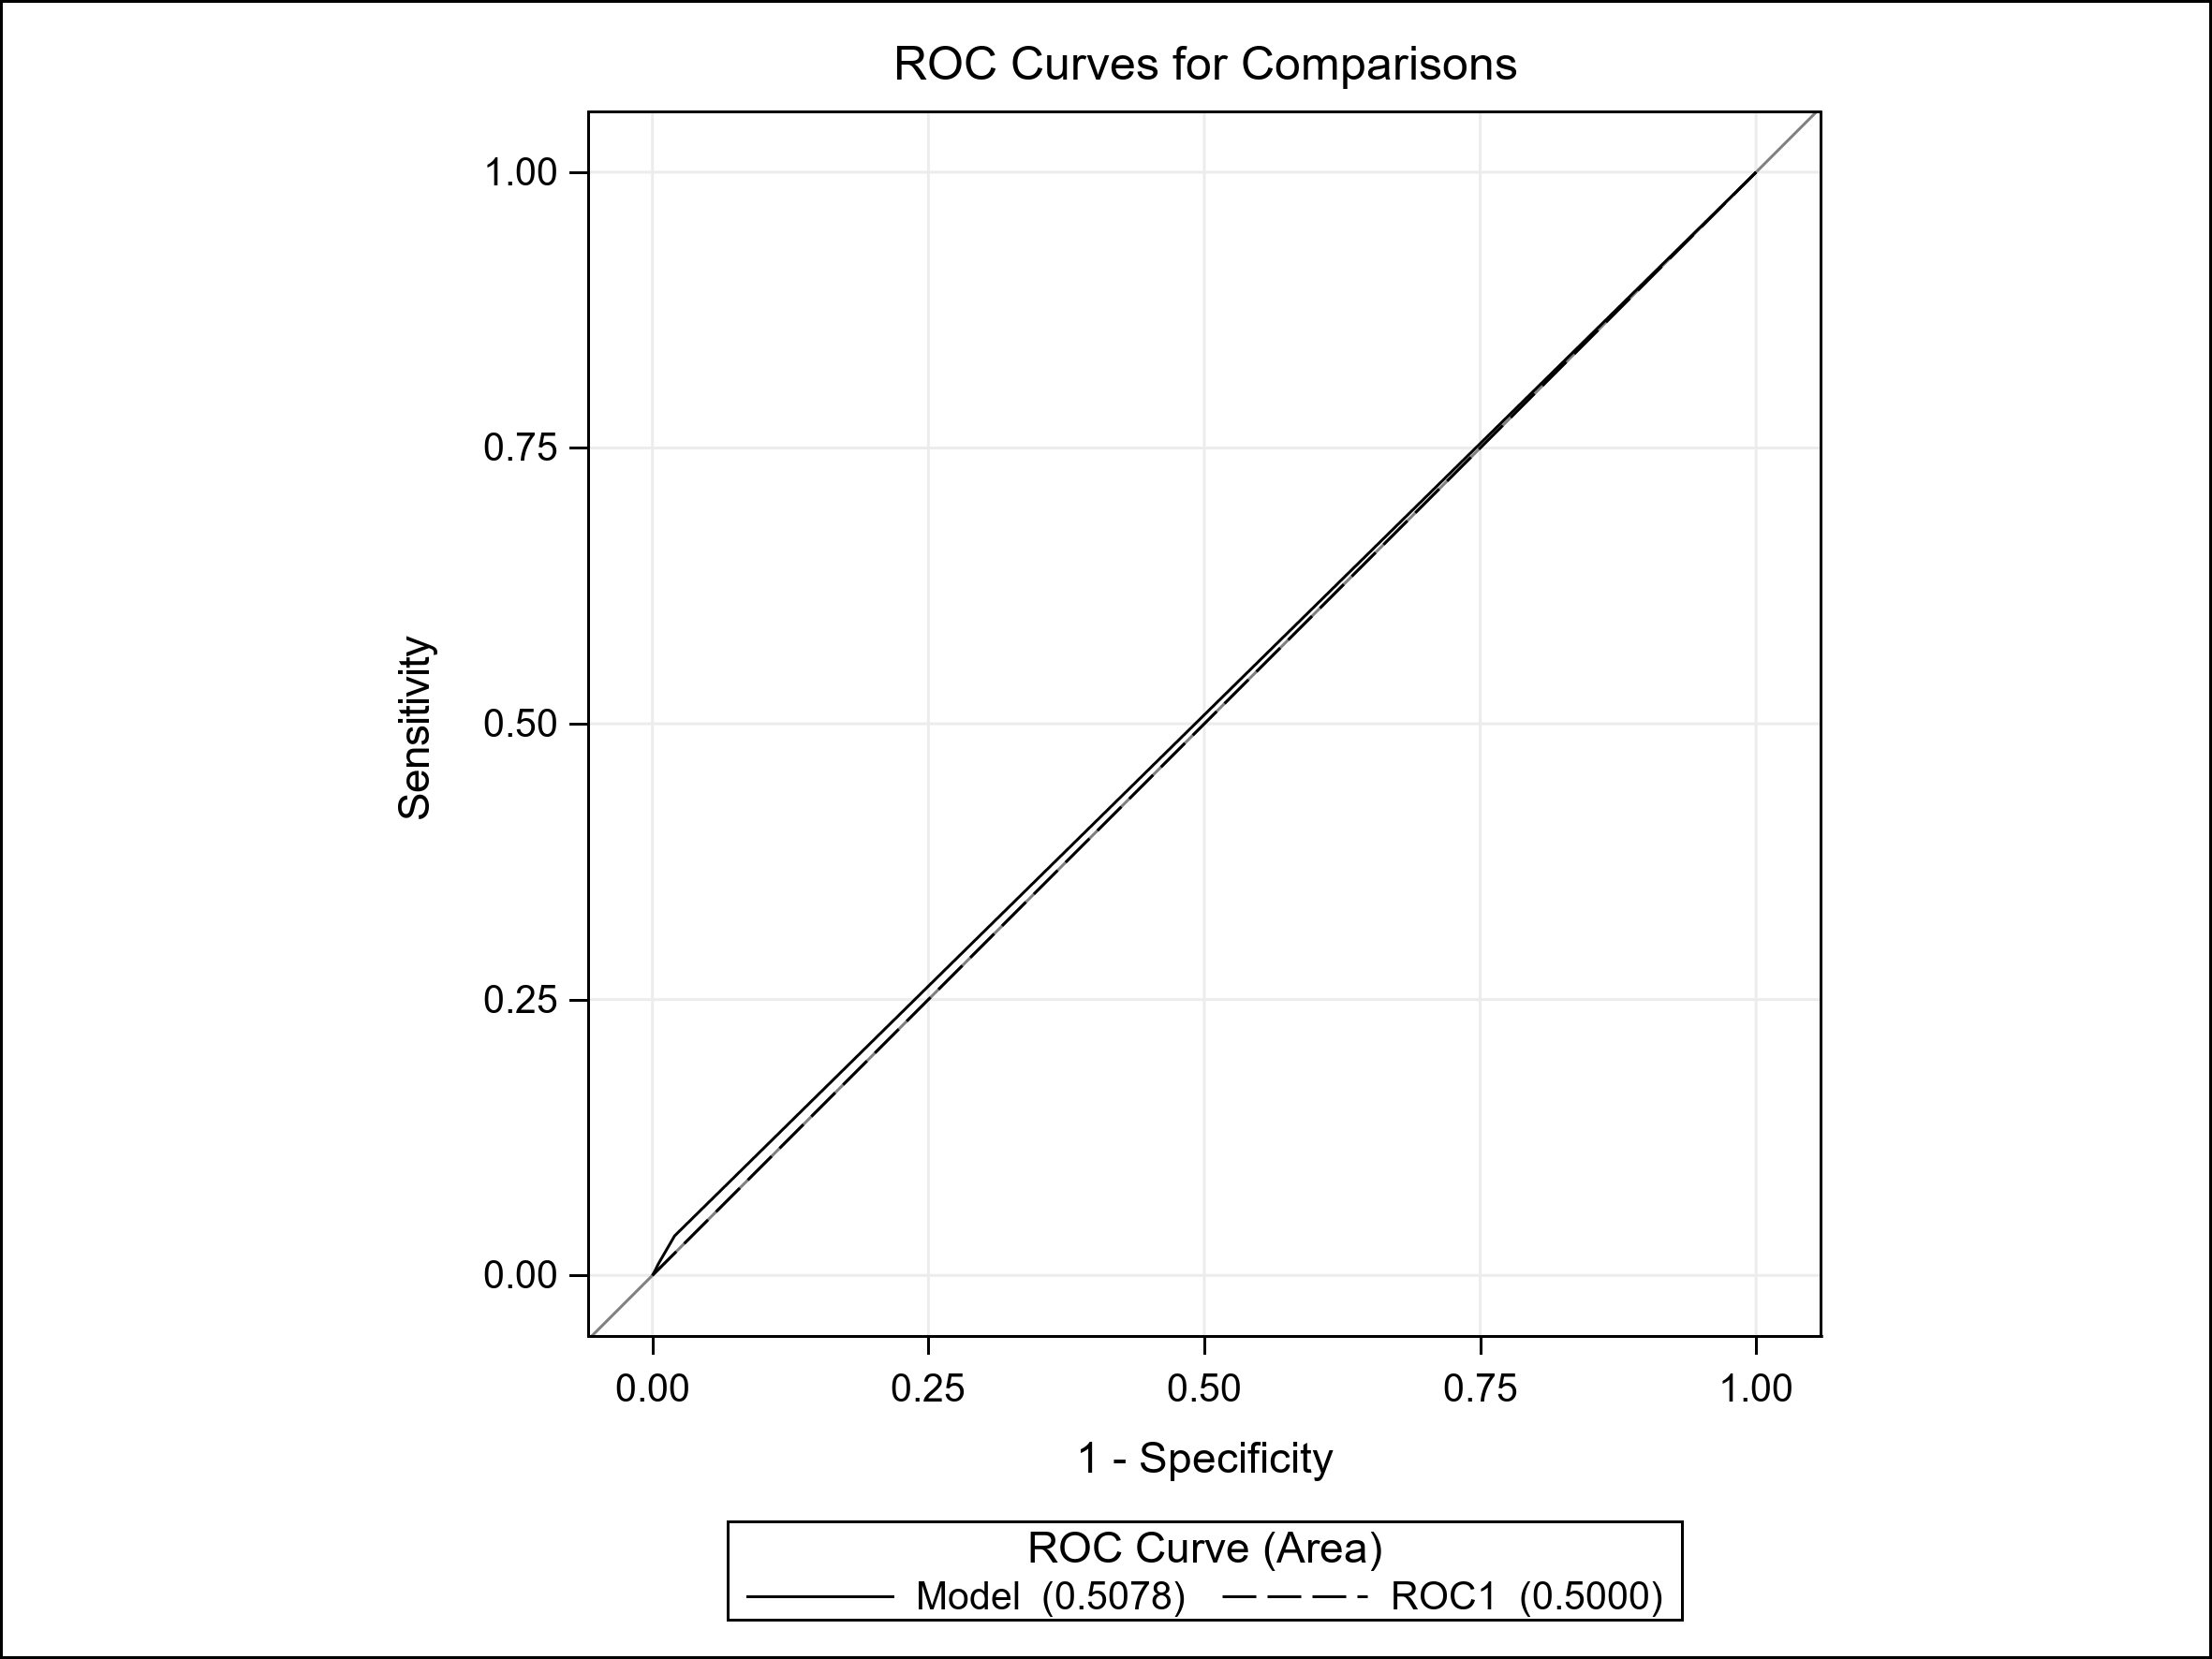
\includegraphics[width=0.5\textwidth]{./plot/ROC/NUM_cnt_units_ROC_ALL5.png}
    \caption{ROC-curve of No Units}
\end{figure}

\subsection{Categorical variables}

\begin{figure}[H]
\begin{minipage}{.5\textwidth}
	\centering
	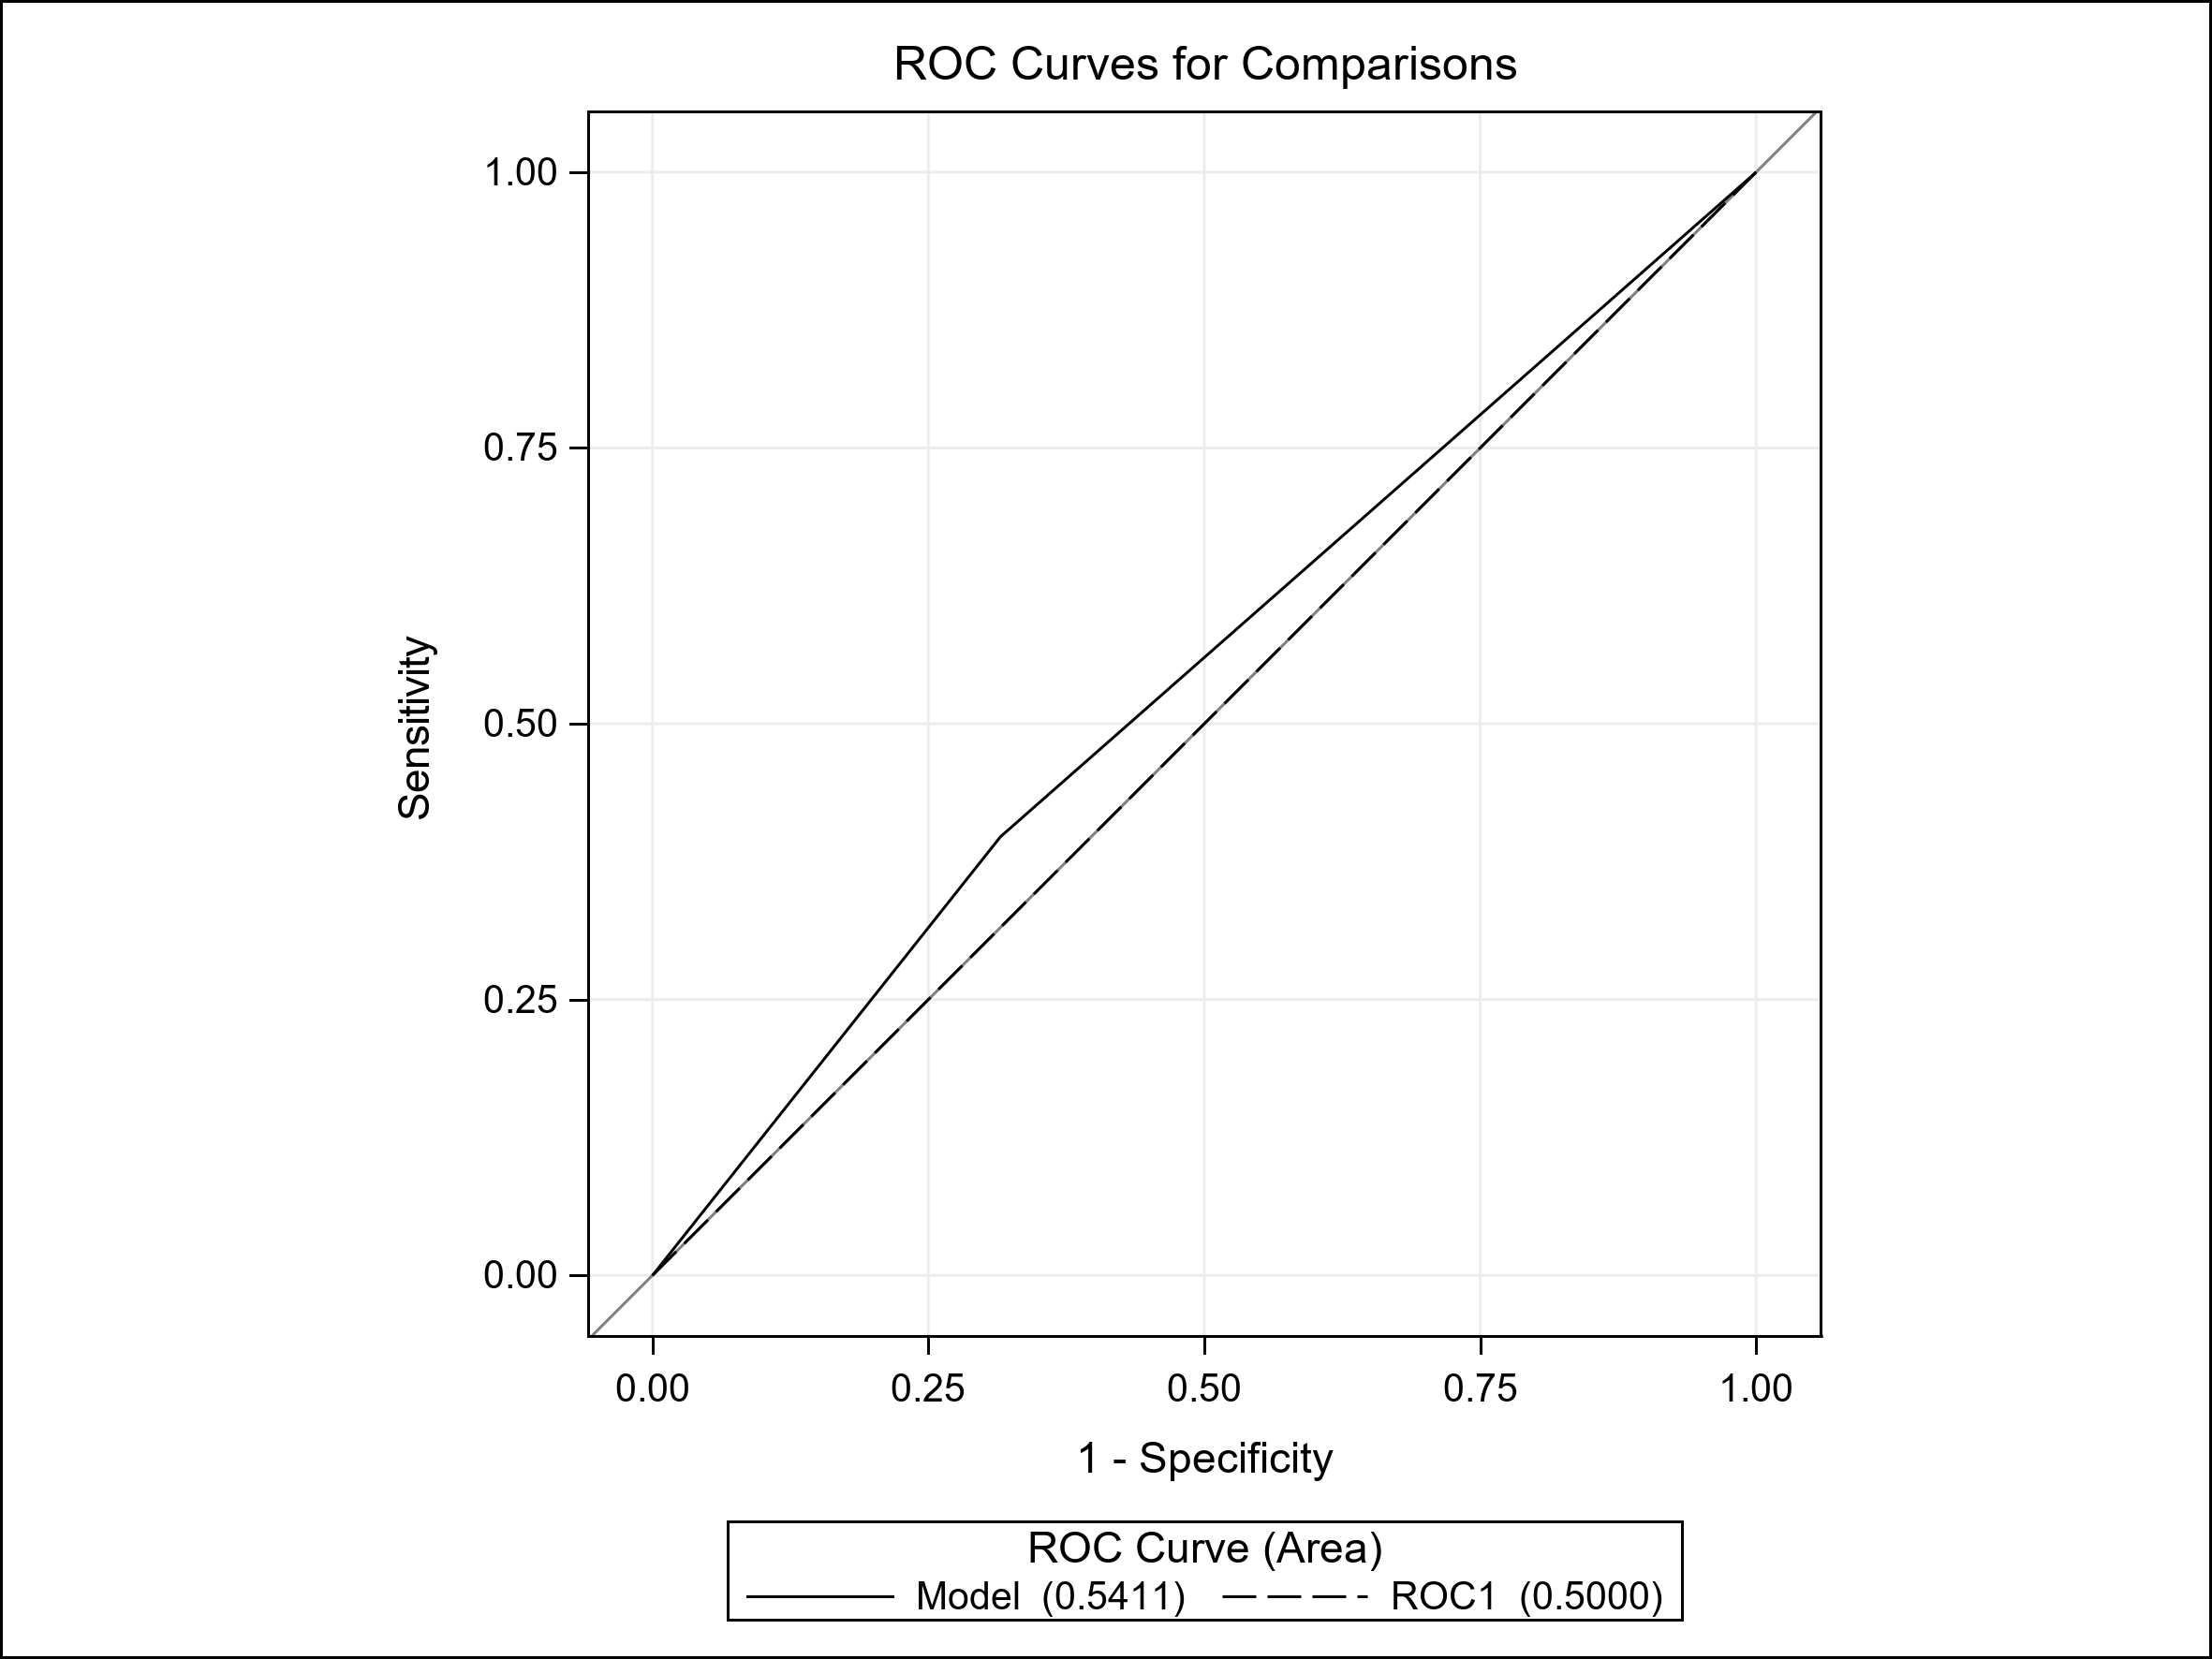
\includegraphics[width=0.9\textwidth]{./plot/ROC/Main/CAT_channel__C_ROC_ALL5.png}
\end{minipage}%
\begin{minipage}{.5\textwidth}
	\centering
	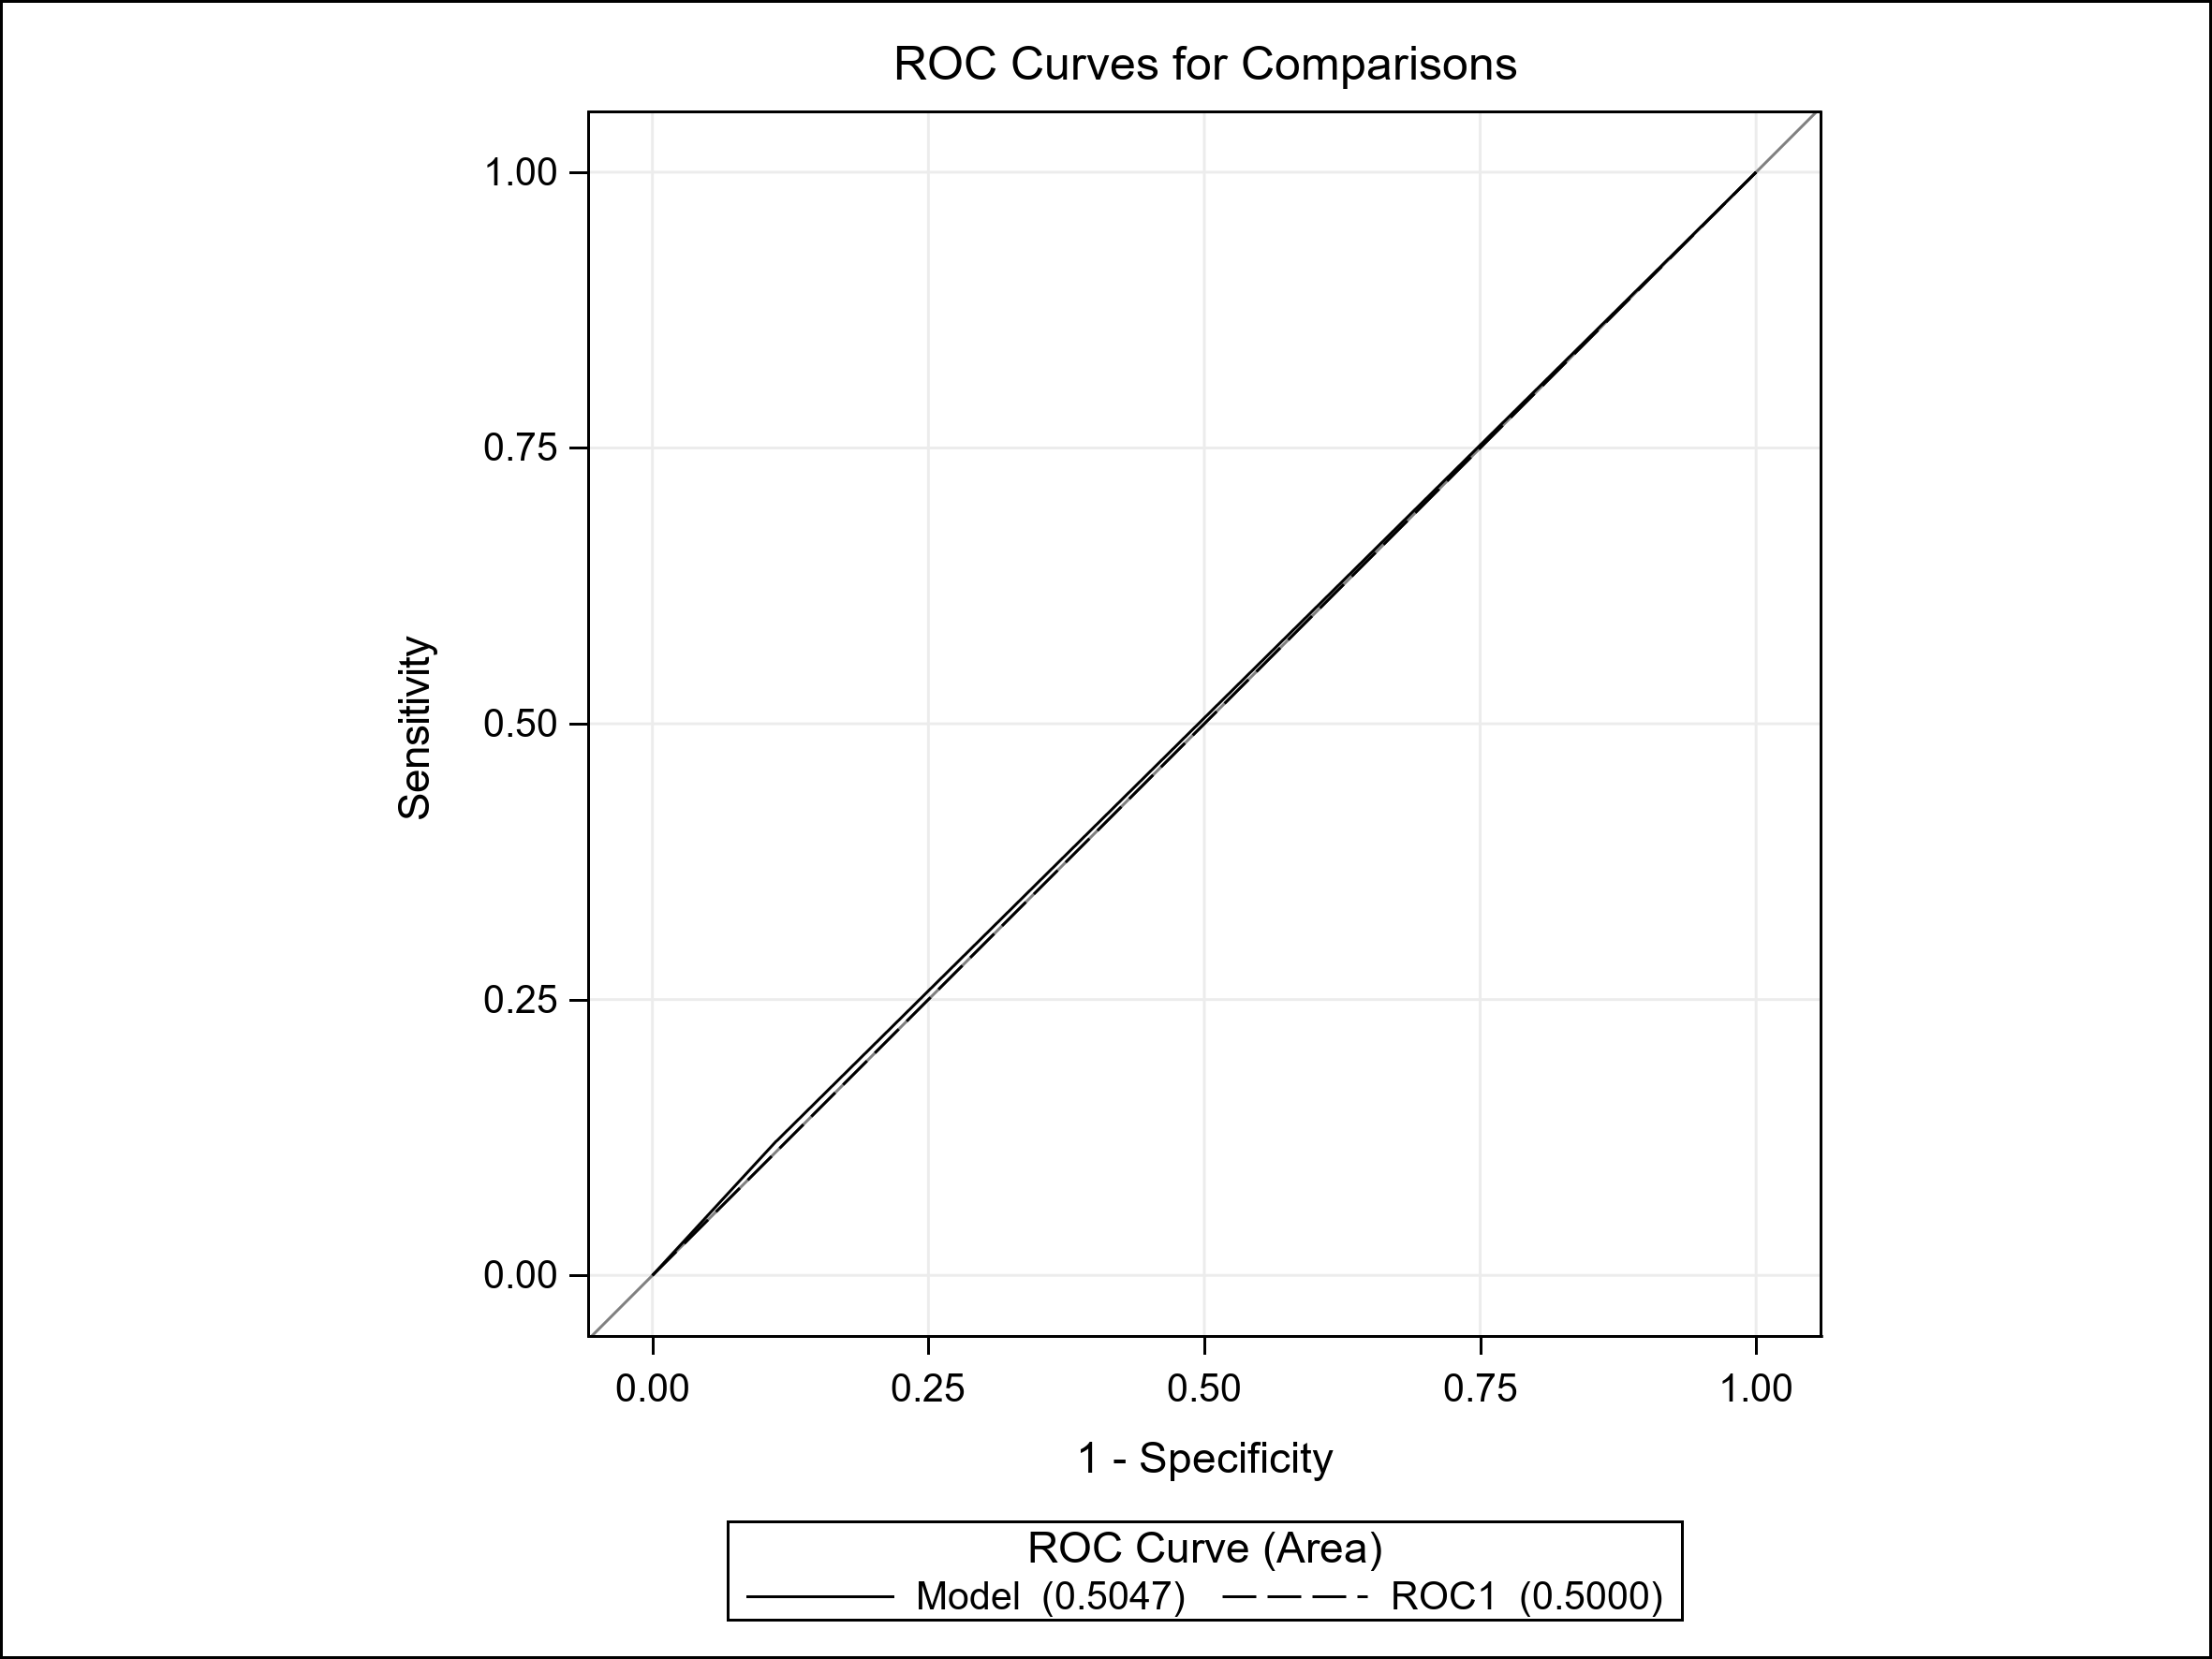
\includegraphics[width=0.9\textwidth]{./plot/ROC/CAT_channel__B_ROC_ALL5.png}
\end{minipage}
    \caption{ROC-curve of Channel = C, B}
\end{figure}

\begin{figure}[H]
\begin{minipage}{.5\textwidth}
	\centering
	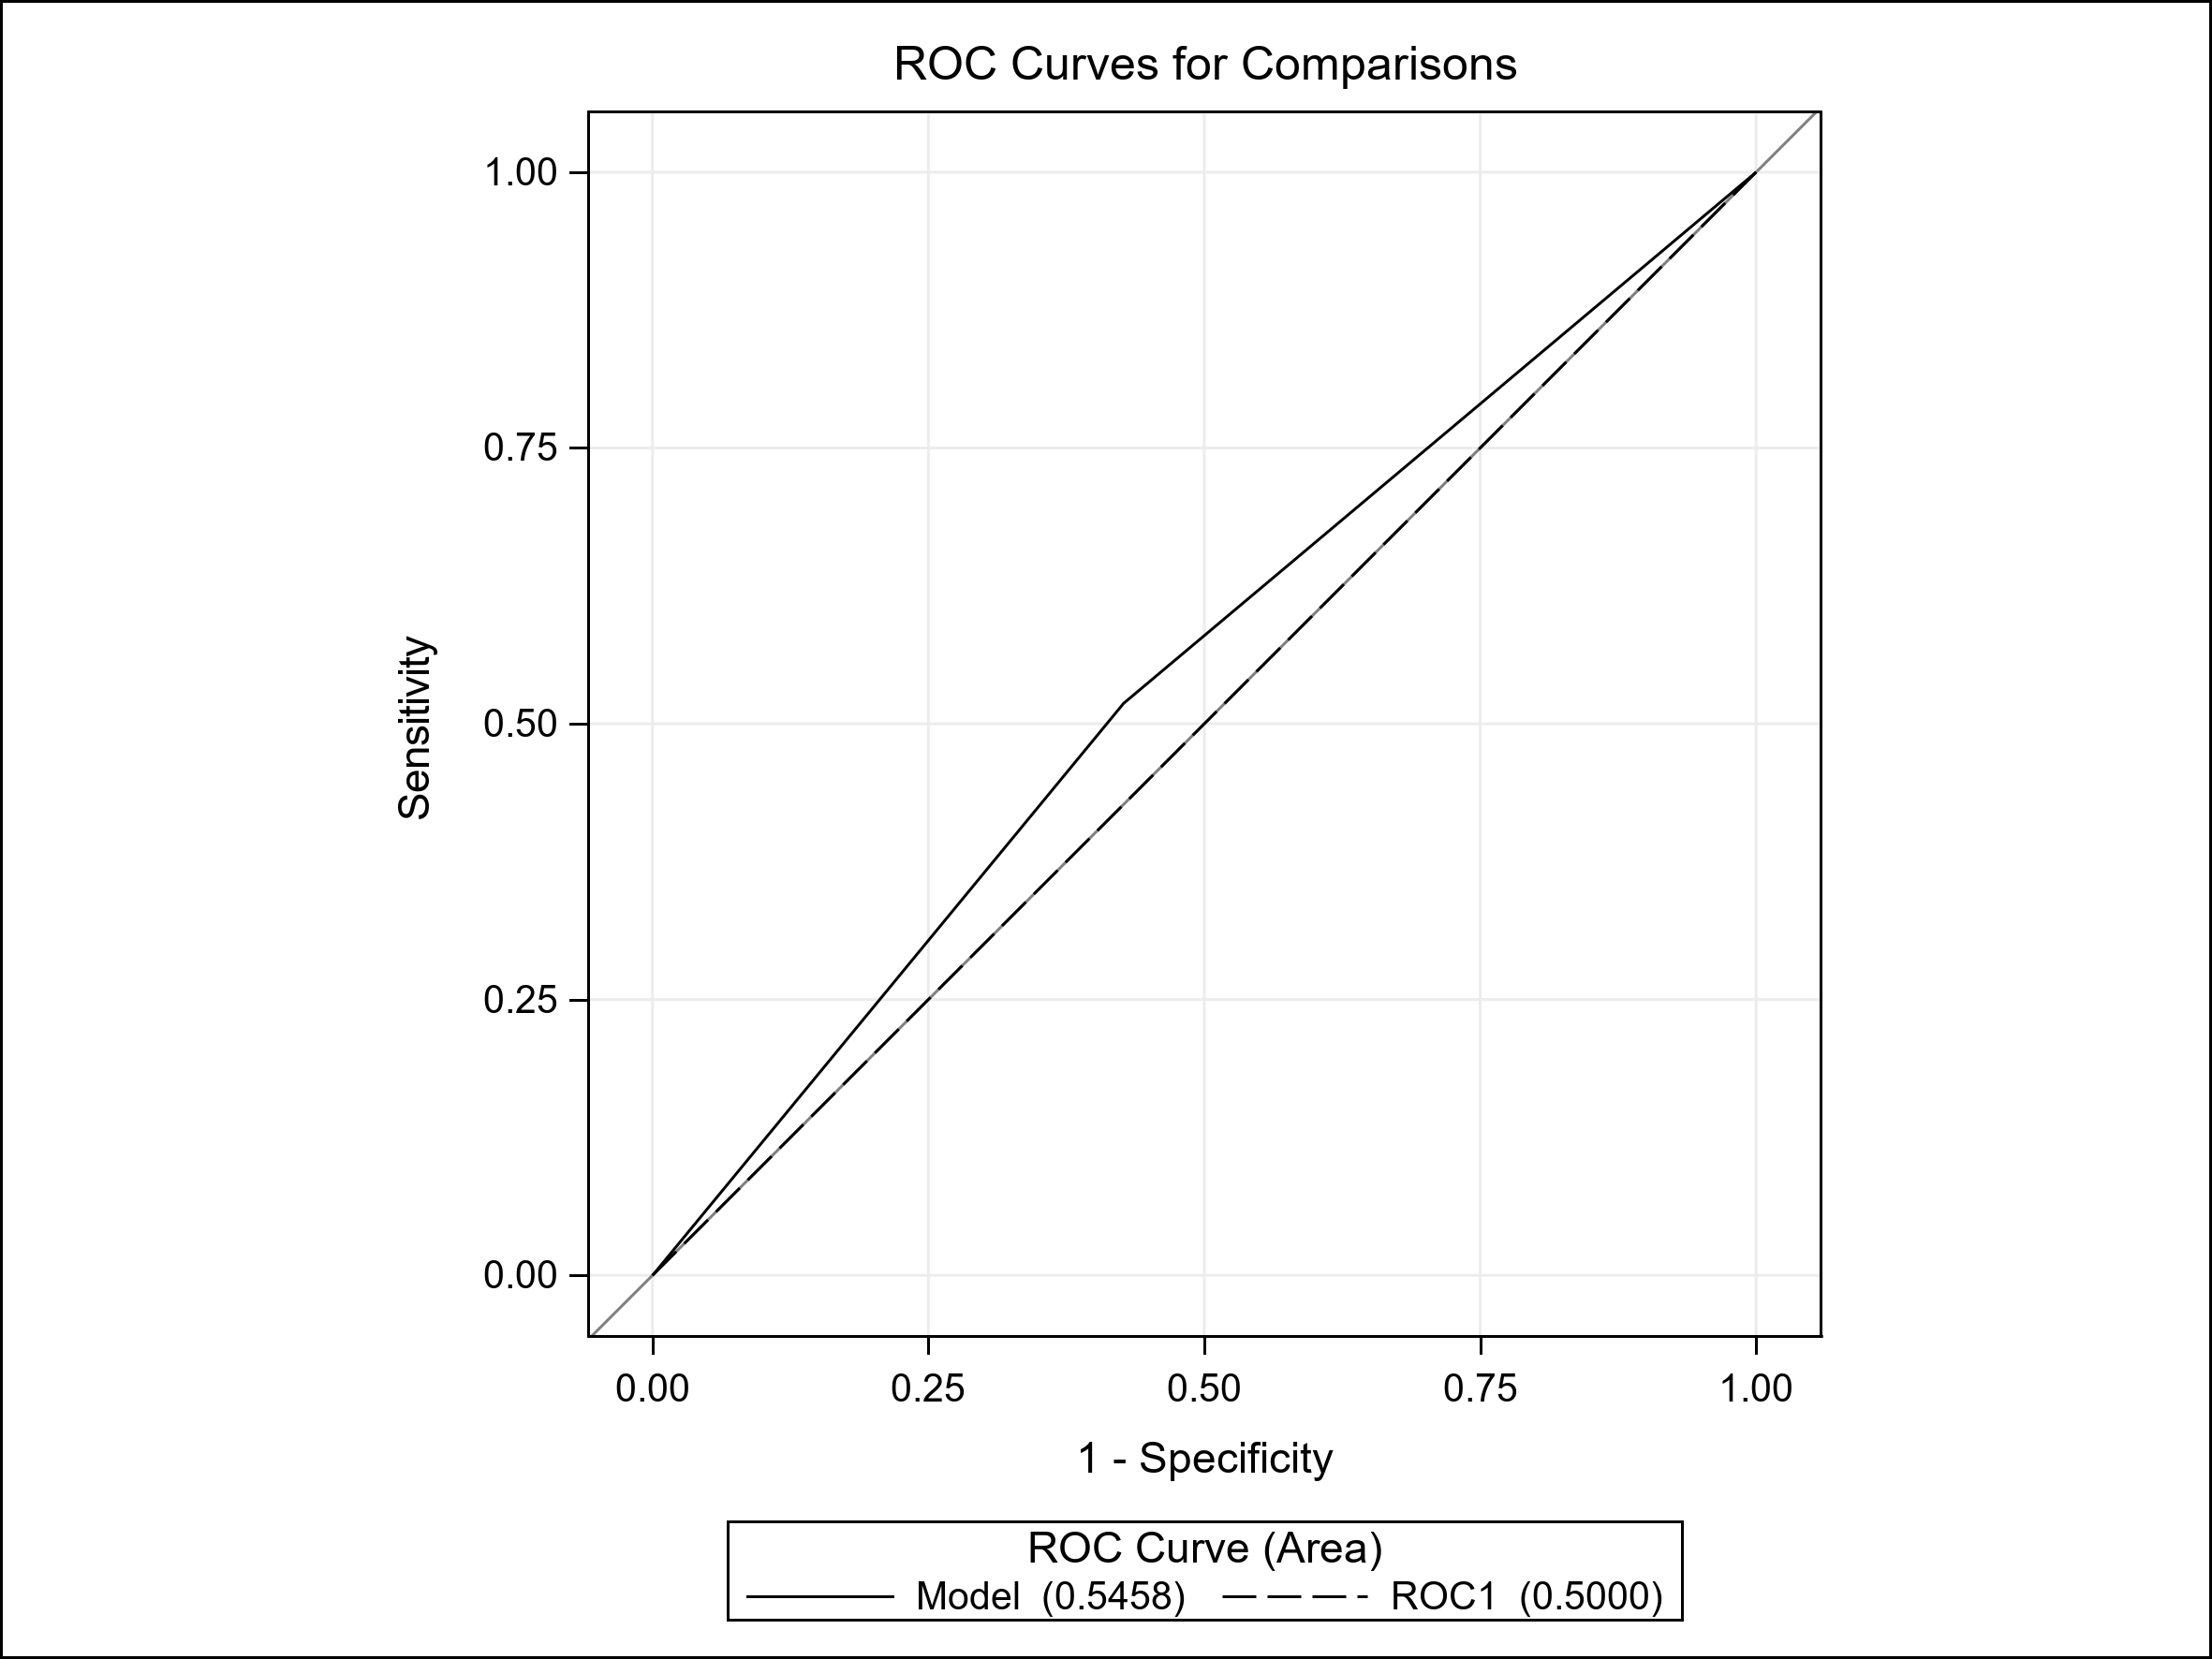
\includegraphics[width=0.9\textwidth]{./plot/ROC/CAT_channel__R_ROC_ALL5.png}
\end{minipage}%
\begin{minipage}{.5\textwidth}
	\centering
	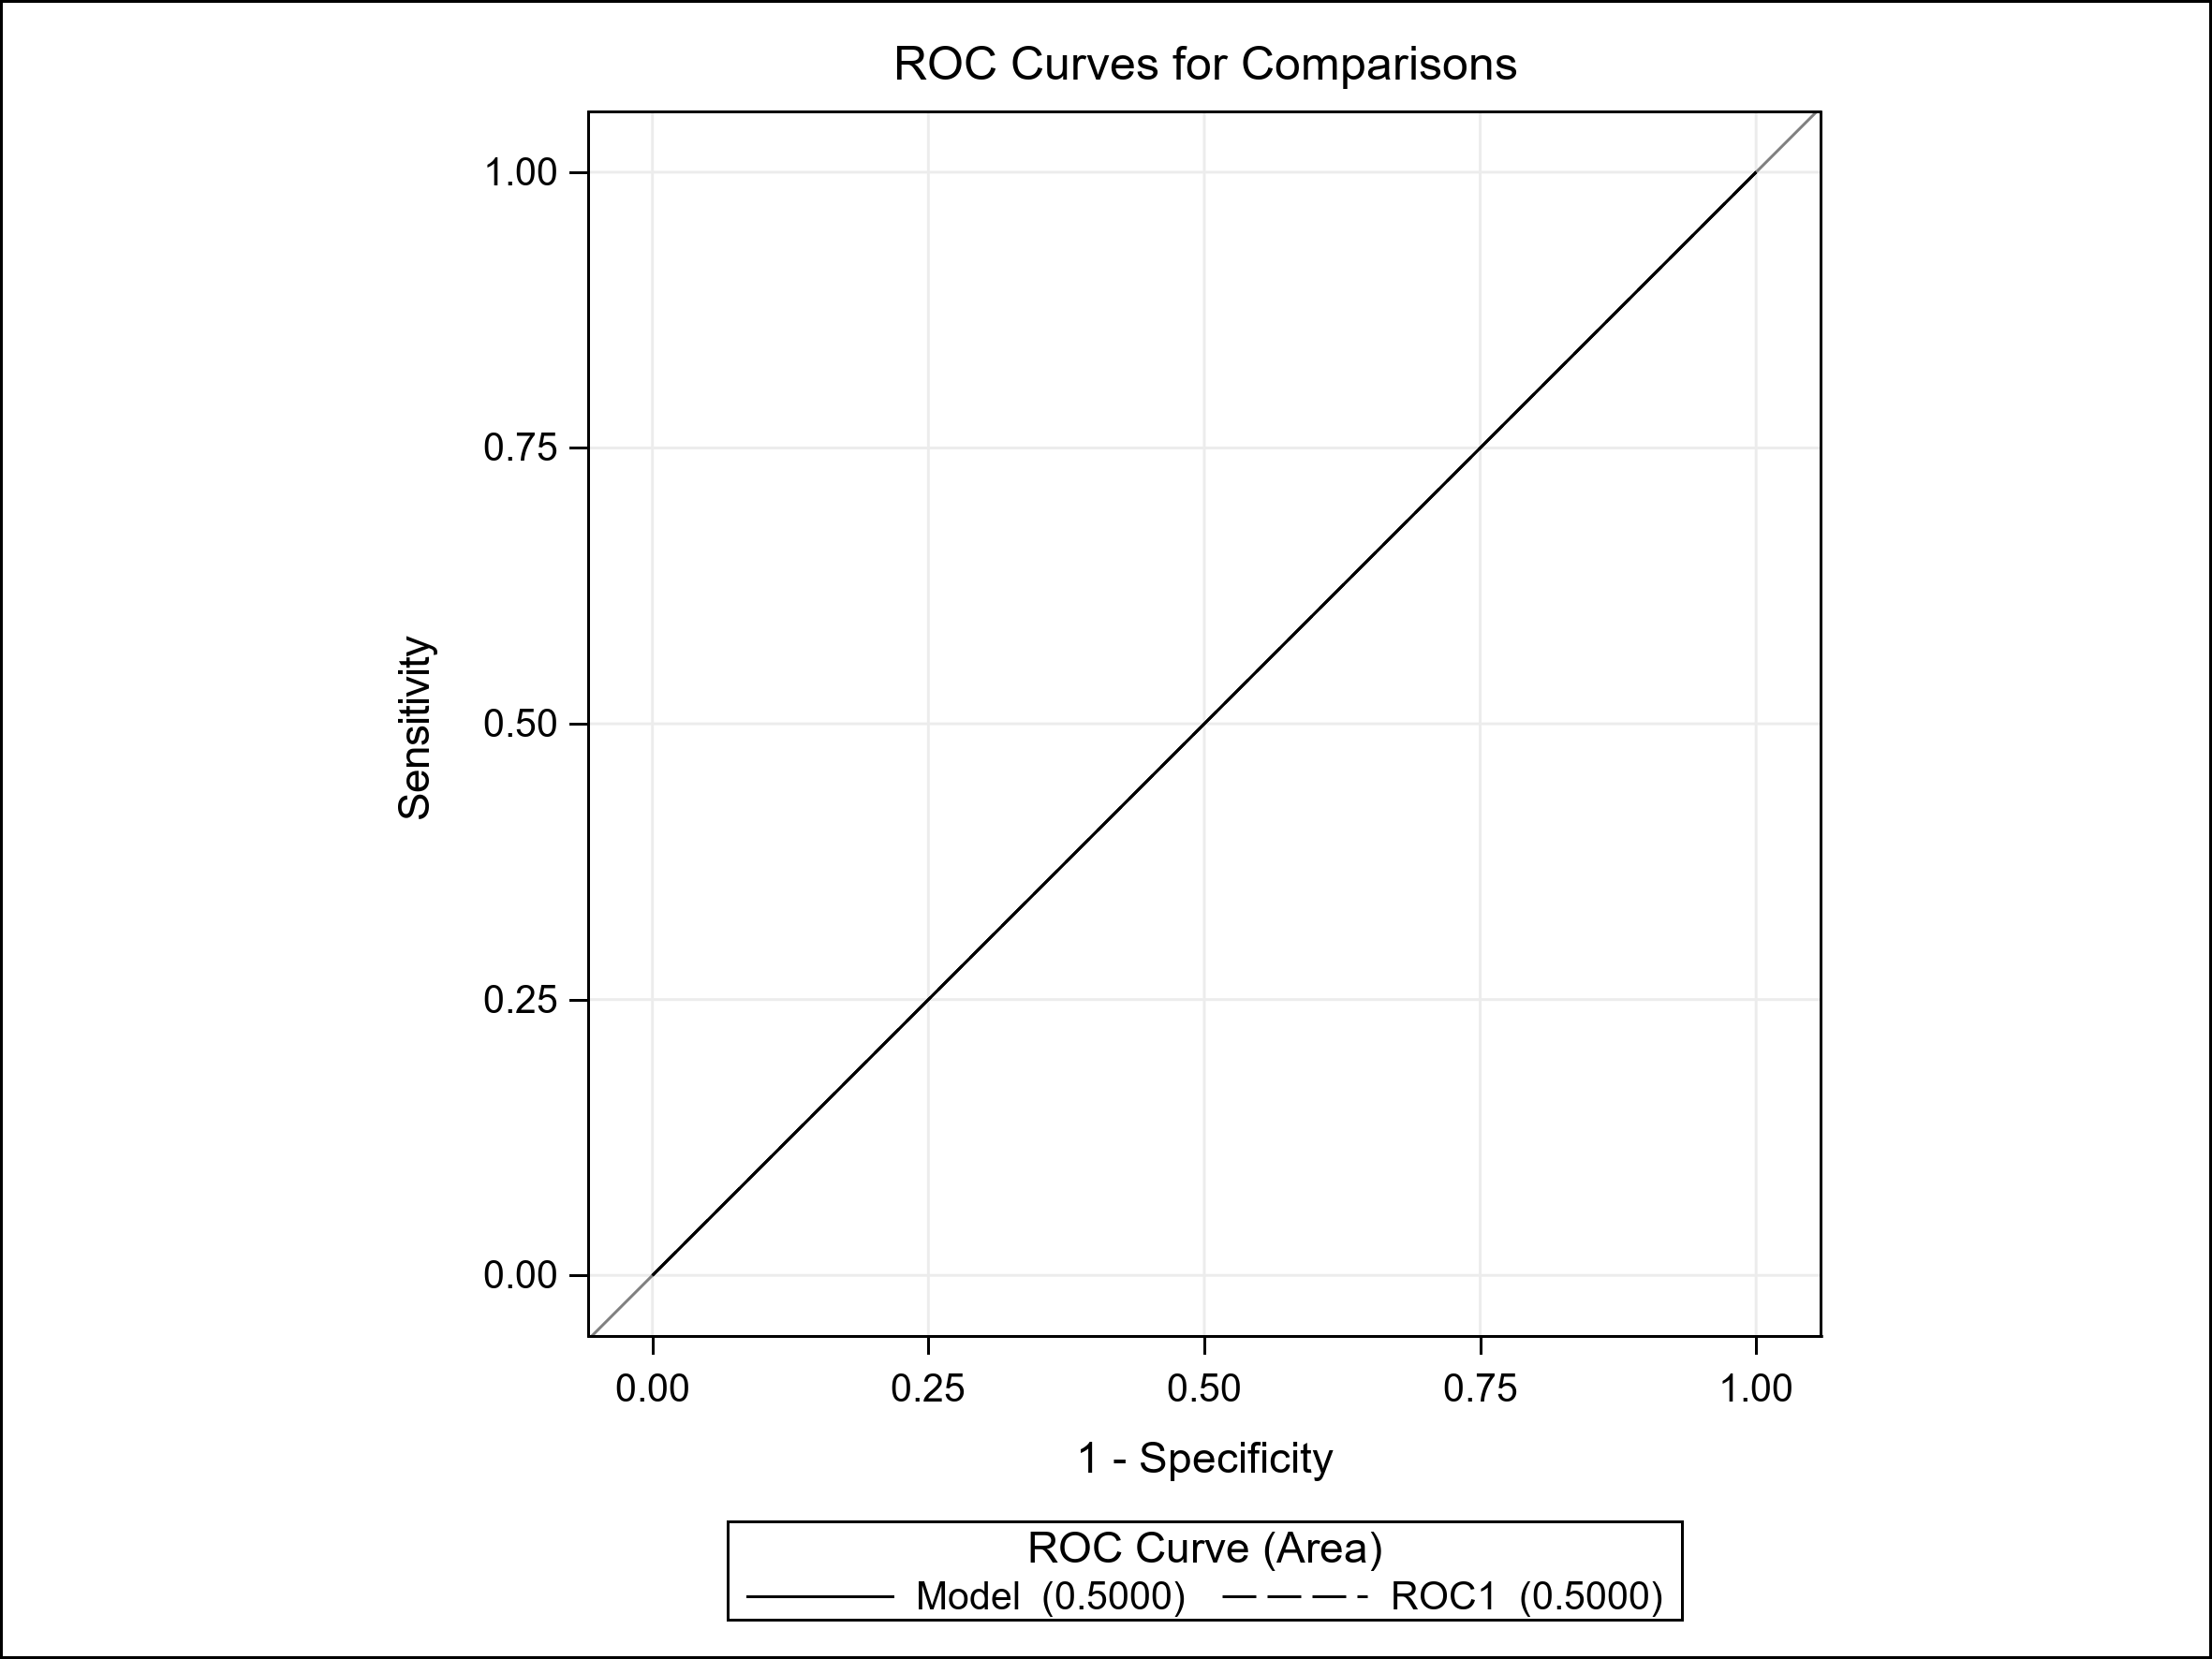
\includegraphics[width=0.9\textwidth]{./plot/ROC/CAT_channel__9_ROC_ALL5.png}
\end{minipage}
    \caption{ROC-curve of Channel = R, Missing}
\end{figure}

\begin{figure}[H]
\begin{minipage}{.5\textwidth}
	\centering
	\includegraphics[width=0.9\textwidth]{./plot/ROC/Main/CAT_us_reg__Midwest_ROC_ALL5.png}
\end{minipage}%
\begin{minipage}{.5\textwidth}
	\centering
	\includegraphics[width=0.9\textwidth]{./plot/ROC/CAT_us_reg__Northeast_ROC_ALL5.png}
\end{minipage}
    \caption{ROC-curve of US Region = Midwest, Northeast}
\end{figure}

\begin{figure}[H]
\begin{minipage}{.5\textwidth}
	\centering
	\includegraphics[width=0.9\textwidth]{./plot/ROC/CAT_us_reg__South_ROC_ALL5.png}
\end{minipage}%
\begin{minipage}{.5\textwidth}
	\centering
	\includegraphics[width=0.9\textwidth]{./plot/ROC/CAT_us_reg__West_ROC_ALL5.png}
\end{minipage}
    \caption{ROC-curve of US Region = South, West}
\end{figure}

\begin{figure}[H]
\begin{minipage}{.5\textwidth}
	\centering
	\includegraphics[width=0.9\textwidth]{./plot/ROC/CAT_us_reg__Other_ROC_ALL5.png}
\end{minipage}%
\begin{minipage}{.5\textwidth}
	\centering
	\includegraphics[width=0.9\textwidth]{./plot/ROC/CAT_occpy_sts__I_ROC_ALL5.png}
\end{minipage}
    \caption{ROC-curve of US Region = Other, Occupancy = I}
\end{figure}

\begin{figure}[H]
\begin{minipage}{.5\textwidth}
	\centering
	\includegraphics[width=0.9\textwidth]{./plot/ROC/CAT_occpy_sts__P_ROC_ALL5.png}
\end{minipage}%
\begin{minipage}{.5\textwidth}
	\centering
	\includegraphics[width=0.9\textwidth]{./plot/ROC/CAT_occpy_sts__S_ROC_ALL5.png}
\end{minipage}
    \caption{ROC-curve of Occupancy = P, S}
\end{figure}

\begin{figure}[H]
\begin{minipage}{.5\textwidth}
	\centering
	\includegraphics[width=0.9\textwidth]{./plot/ROC/CAT_cd_ppty_val_type__1_ROC_ALL5.png}
\end{minipage}%
\begin{minipage}{.5\textwidth}
	\centering
	\includegraphics[width=0.9\textwidth]{./plot/ROC/CAT_cd_ppty_val_type__2_ROC_ALL5.png}
\end{minipage}
    \caption{ROC-curve of Prop Val Method = 1, 2}
\end{figure}

\begin{figure}[H]
\begin{minipage}{.5\textwidth}
	\centering
	\includegraphics[width=0.9\textwidth]{./plot/ROC/CAT_cd_ppty_val_type__3_ROC_ALL5.png}
\end{minipage}%
\begin{minipage}{.5\textwidth}
	\centering
	\includegraphics[width=0.9\textwidth]{./plot/ROC/CAT_cd_ppty_val_type__9_ROC_ALL5.png}
\end{minipage}
    \caption{ROC-curve of Prop Val Method = 3, Missing}
\end{figure}

\begin{figure}[H]
\begin{minipage}{.5\textwidth}
	\centering
	\includegraphics[width=0.9\textwidth]{./plot/ROC/CAT_ind_afdl__F_ROC_ALL5.png}
\end{minipage}%
\begin{minipage}{.5\textwidth}
	\centering
	\includegraphics[width=0.9\textwidth]{./plot/ROC/CAT_ind_afdl__H_ROC_ALL5.png}
\end{minipage}
    \caption{ROC-curve of Prog Flag = F, H}
\end{figure}

\begin{figure}[H]
\begin{minipage}{.5\textwidth}
	\centering
	\includegraphics[width=0.9\textwidth]{./plot/ROC/CAT_ind_afdl__9_ROC_ALL5.png}
\end{minipage}%
\begin{minipage}{.5\textwidth}
	\centering
	\includegraphics[width=0.9\textwidth]{./plot/ROC/CAT_amrtzn_type__FRM_ROC_ALL5.png}
\end{minipage}
    \caption{ROC-curve of Prog Flag = Missing and Amort Type = FRM}
\end{figure}


\begin{figure}[H]
\begin{minipage}{.5\textwidth}
	\centering
	\includegraphics[width=0.9\textwidth]{./plot/ROC/CAT_prop_type__CO_ROC_ALL5.png}
\end{minipage}%
\begin{minipage}{.5\textwidth}
	\centering
	\includegraphics[width=0.9\textwidth]{./plot/ROC/CAT_prop_type__CP_ROC_ALL5.png}
\end{minipage}
    \caption{ROC-curve of Prop Type = CO, CP}
\end{figure}

\begin{figure}[H]
\begin{minipage}{.5\textwidth}
	\centering
	\includegraphics[width=0.9\textwidth]{./plot/ROC/CAT_prop_type__MH_ROC_ALL5.png}
\end{minipage}%
\begin{minipage}{.5\textwidth}
	\centering
	\includegraphics[width=0.9\textwidth]{./plot/ROC/CAT_prop_type__PU_ROC_ALL5.png}
\end{minipage}
    \caption{ROC-curve of Prop Type = MH, PU}
\end{figure}

\begin{figure}[H]
\begin{minipage}{.5\textwidth}
	\centering
	\includegraphics[width=0.9\textwidth]{./plot/ROC/CAT_prop_type__SF_ROC_ALL5.png}
\end{minipage}%
\begin{minipage}{.5\textwidth}
	\centering
	\includegraphics[width=0.9\textwidth]{./plot/ROC/CAT_orig_loan_term_3grp__EQ_360M_ROC_ALL5.png}
\end{minipage}
    \caption{ROC-curve of Prop Type = SF and Loan Term = 360m}
\end{figure}

\begin{figure}[H]
\begin{minipage}{.5\textwidth}
	\centering
	\includegraphics[width=0.9\textwidth]{./plot/ROC/CAT_orig_loan_term_3grp__HI_360M_ROC_ALL5.png}
\end{minipage}%
\begin{minipage}{.5\textwidth}
	\centering
	\includegraphics[width=0.9\textwidth]{./plot/ROC/CAT_orig_loan_term_3grp__LE_360M_ROC_ALL5.png}
\end{minipage}
    \caption{ROC-curve of Loan Term > 360m, < 360m}
\end{figure}

\subsection{Indicator variables}

\begin{figure}[H]
\begin{minipage}{.5\textwidth}
	\centering
	\includegraphics[width=0.9\textwidth]{./plot/ROC/Main/IND_flag_orig_loan_term_HEQ_360M_ROC_ALL5.png}
\end{minipage}%
\begin{minipage}{.5\textwidth}
	\centering
	\includegraphics[width=0.9\textwidth]{./plot/ROC/IND_flag_cnt_units_ROC_ALL5.png}
\end{minipage}
    \caption{ROC-curve of Loan Term $\geq$ 360m and Flag Number of units}
\end{figure}

\begin{figure}[H]
\begin{minipage}{.5\textwidth}
	\centering
	\includegraphics[width=0.9\textwidth]{./plot/ROC/IND_flag_fthb_ROC_ALL5.png}
\end{minipage}%
\begin{minipage}{.5\textwidth}
	\centering
	\includegraphics[width=0.9\textwidth]{./plot/ROC/IND_flag_int_only_ROC_ALL5.png}
\end{minipage}
    \caption{ROC-curve of Homebuyer Flag and Int Only Flag}
\end{figure}

\begin{figure}[H]
\begin{minipage}{.5\textwidth}
	\centering
	\includegraphics[width=0.9\textwidth]{./plot/ROC/IND_flag_mi_ROC_ALL5.png}
\end{minipage}%
\begin{minipage}{.5\textwidth}
	\centering
	\includegraphics[width=0.9\textwidth]{./plot/ROC/IND_flag_sc_ROC_ALL5.png}
\end{minipage}
    \caption{ROC-curve of MI Flag and Sup Conf Flag}
\end{figure}

\begin{figure}[H]
\begin{minipage}{.5\textwidth}
	\centering
	\includegraphics[width=0.9\textwidth]{./plot/ROC/IND_ind_harp_ROC_ALL5.png}
\end{minipage}%
\begin{minipage}{.5\textwidth}
	\centering
	\includegraphics[width=0.9\textwidth]{./plot/ROC/IND_ppmt_pnlty_ROC_ALL5.png}
\end{minipage}
    \caption{ROC-curve of HARP Flag and PPM Flag}
\end{figure}

\begin{figure}[H]
\begin{minipage}{.5\textwidth}
	\centering
	\includegraphics[width=0.9\textwidth]{./plot/ROC/IND_flag_orig_loan_term_EQ_360M_ROC_ALL5.png}
\end{minipage}%
\begin{minipage}{.5\textwidth}
	\centering
	\includegraphics[width=0.9\textwidth]{./plot/ROC/IND_flag_orig_loan_term_HI_360M_ROC_ALL5.png}
\end{minipage}
    \caption{ROC-curve of Flag Loan Term = 360m and Loan Term > 360m}
\end{figure}

\section{Partial Dependence Display of all model variables}
\label{sec:PDP_all}

\subsection{Numerical variables}

\begin{figure}[H]
\begin{minipage}{.5\textwidth}
	\centering
	\includegraphics[width=0.9\textwidth]{./plot/ML/PDP_fico.png}
\end{minipage}%
\begin{minipage}{.5\textwidth}
	\centering
	\includegraphics[width=0.9\textwidth]{./plot/ML/PDP_orig_upb.png}
\end{minipage}
    \caption{PDP of Credit Score and UPB}
\end{figure}

\begin{figure}[H]
\begin{minipage}{.5\textwidth}
	\centering
	\includegraphics[width=0.9\textwidth]{./plot/ML/PDP_ltv.png}
\end{minipage}%
\begin{minipage}{.5\textwidth}
	\centering
	\includegraphics[width=0.9\textwidth]{./plot/ML/PDP_cltv.png}
\end{minipage}
    \caption{PDP of LTV and CLTV}
\end{figure}

\begin{figure}[H]
\begin{minipage}{.5\textwidth}
	\centering
	\includegraphics[width=0.9\textwidth]{./plot/ML/PDP_dti.png}
\end{minipage}%
\begin{minipage}{.5\textwidth}
	\centering
	\includegraphics[width=0.9\textwidth]{./plot/ML/PDP_mi_pct.png}
\end{minipage}
    \caption{PDP of DTI and MI Perc}
\end{figure}

\begin{figure}[H]
\begin{minipage}{.5\textwidth}
	\centering
	\includegraphics[width=0.9\textwidth]{./plot/ML/PDP_cnt_borr.png}
\end{minipage}%
\begin{minipage}{.5\textwidth}
	\centering
	\includegraphics[width=0.9\textwidth]{./plot/ML/PDP_cnt_units.png}
\end{minipage}
    \caption{PDP of No Borrowers and No Units}
\end{figure}

\begin{figure}[H]
	\centering
	\includegraphics[width=0.5\textwidth]{./plot/ML/PDP_orig_loan_term.png}
    \caption{PDP of Loan Term}
\end{figure}

\subsection{Categorical variables}

\begin{figure}[H]
\begin{minipage}{.5\textwidth}
	\centering
	\includegraphics[width=0.9\textwidth]{./plot/ML/PDP_us_reg__Midwest.png}
\end{minipage}%
\begin{minipage}{.5\textwidth}
	\centering
	\includegraphics[width=0.9\textwidth]{./plot/ML/PDP_us_reg__Northeast.png}
\end{minipage}
    \caption{PDP of US Region = Midwest, Northeast}
\end{figure}

\begin{figure}[H]
\begin{minipage}{.5\textwidth}
	\centering
	\includegraphics[width=0.9\textwidth]{./plot/ML/PDP_us_reg__South.png}
\end{minipage}%
\begin{minipage}{.5\textwidth}
	\centering
	\includegraphics[width=0.9\textwidth]{./plot/ML/PDP_us_reg__West.png}
\end{minipage}
    \caption{PDP of US Region = South, West}
\end{figure}

\begin{figure}[H]
\begin{minipage}{.5\textwidth}
	\centering
	\includegraphics[width=0.9\textwidth]{./plot/ML/PDP_us_reg__Other.png}
\end{minipage}%
\begin{minipage}{.5\textwidth}
	\centering
	\includegraphics[width=0.9\textwidth]{./plot/ML/PDP_channel__B.png}
\end{minipage}
    \caption{PDP of US Region = Other and Channel = B}
\end{figure}

\begin{figure}[H]
\begin{minipage}{.5\textwidth}
	\centering
	\includegraphics[width=0.9\textwidth]{./plot/ML/PDP_channel__R.png}
\end{minipage}%
\begin{minipage}{.5\textwidth}
	\centering
	\includegraphics[width=0.9\textwidth]{./plot/ML/PDP_channel__9.png}
\end{minipage}
    \caption{PDP of Channel = R, Missing}
\end{figure}

\begin{figure}[H]
\begin{minipage}{.5\textwidth}
	\centering
	\includegraphics[width=0.9\textwidth]{./plot/ML/PDP_loan_purpose__C.png}
\end{minipage}%
\begin{minipage}{.5\textwidth}
	\centering
	\includegraphics[width=0.9\textwidth]{./plot/ML/PDP_loan_purpose__N.png}
\end{minipage}
    \caption{PDP of Loan Purpose = P = C, N}
\end{figure}

\begin{figure}[H]
\begin{minipage}{.5\textwidth}
	\centering
	\includegraphics[width=0.9\textwidth]{./plot/ML/PDP_loan_purpose__P.png}
\end{minipage}%
\begin{minipage}{.5\textwidth}
	\centering
	\includegraphics[width=0.9\textwidth]{./plot/ML/PDP_cd_ppty_val_type__1.png}
\end{minipage}
    \caption{PDP of Loan Purpose = P and Prop Val Method = 1}
\end{figure}

\begin{figure}[H]
\begin{minipage}{.5\textwidth}
	\centering
	\includegraphics[width=0.9\textwidth]{./plot/ML/PDP_cd_ppty_val_type__2.png}
\end{minipage}%
\begin{minipage}{.5\textwidth}
	\centering
	\includegraphics[width=0.9\textwidth]{./plot/ML/PDP_cd_ppty_val_type__3.png}
\end{minipage}
    \caption{PDP of Prop Val Method = 2,3}
\end{figure}

\begin{figure}[H]
	\centering
	\includegraphics[width=0.5\textwidth]{./plot/ML/PDP_cd_ppty_val_type__9.png}
    \caption{PDP of Prop Val Method = Not Available}
\end{figure}

\subsection{Indicator variables}

\begin{figure}[H]
\begin{minipage}{.5\textwidth}
	\centering
	\includegraphics[width=0.9\textwidth]{./plot/ML/PDP_flag_mi.png}
\end{minipage}%
\begin{minipage}{.5\textwidth}
	\centering
	\includegraphics[width=0.9\textwidth]{./plot/ML/PDP_flag_orig_loan_term_HEQ_360M.png}
\end{minipage}
    \caption{PDP of MI Flag and Loan Term $\geq$ 360m}
\end{figure}